\documentclass[ngerman, paper=a4, 12pt]{scrartcl}
\usepackage[utf8]{inputenc}
\usepackage{babel}
\usepackage[T1]{fontenc}
\usepackage{lmodern}

\usepackage{amssymb}
\usepackage{amsmath}
\usepackage{mathrsfs}
\usepackage{amsfonts}
\usepackage{dsfont}
\usepackage{braket}
\usepackage{tabularx}
\usepackage{mathtools}
\usepackage{graphicx}
\usepackage{marginnote}
\usepackage{float}
\usepackage{empheq}
\usepackage{placeins}
\usepackage{color}
\usepackage{enumerate}
\usepackage[colorlinks=true, linkcolor=cyan]{hyperref}

\newcommand{\diff}{\mathrm{d}}
\newcommand{\U}{\mathcal{U}}
\newcommand{\T}{\mathrm{T}}
\newcommand{\Hil}{\mathcal{H}}

\newcommand{\Erw}[1]{\left\langle {#1} \right\rangle}
\newcommand{\erw}[1]{\langle {#1} \rangle}


\begin{document}
\tableofcontents
\newpage
\setcounter{section}{-1}
%\numberwithin{equation}{section}
	
	%Kap 0
	\section{Quantenmechanik}
	\marginpar{12.10.2015}
	\subsection{Mechanik}
		Der einfachste Lagrange lautet 
			\begin{equation*}
				L (x,\dot{x}) = \frac{m}{2} \dot{x}^2 - V(x) 
			\end{equation*}
		Um jetzt die Hamiltonfunktion zu konstruieren, schreiben wir:
			\begin{equation*}
				p=
				\frac{\partial L}{\partial \dot{x}}
				(=m \dot{x})
			\end{equation*}
		Sodass
			\begin{equation*}
				H(x,p)= 
				p \dot{x} - L(x,\dot{x}) = 
				\frac{p^2}{2m} + V(x)
			\end{equation*}
		Poisson-Klammern:
			\begin{equation*}
				\{A,B\}=
				\frac{\partial A}{\partial x} \frac{\partial B}{\partial p}
				- \frac{\partial B}{\partial x} \frac{\partial A}{\partial p}
			\end{equation*}
		Beispiele mit Spezialfällen:
		\begin{tabbing}
			\hspace{0.4\linewidth} \= \hspace{0.6\linewidth} \= \hfill \kill
			$\frac{\diff F}{dt} = \dot{F} = \{F,H\} + \frac{\partial F}{\partial t}$ \> 
			Phasenraumfunktion $F(x,p,t)$ \\ \\
			$\frac{\diff H}{dt} = \{H,H\} + \frac{\partial H}{\partial t} = \frac{\partial H}{\partial t}$ \>
			Falls $H$ nicht explizit zeitabhängig, dann ist Energie \\
			\hfill \>  in H erhalten. \\  %Unschöne Lösung
			$\frac{\diff x}{\diff t} = \{x,H\} = \frac{\partial H}{\partial p}$ \>
			$=\frac{p}{m} \rightarrow$ Geschwindigkeit ist Impuls durch Masse. \\ \\
			$\frac{\diff p}{\diff t} = \{p,H\} = -\frac{\partial H}{\partial x}$ \>
			Newton: $F= ma= \dot{p} =$``$- \nabla V$''	
		\end{tabbing}
		Fundamentale Poissonklammern:
			\begin{align*}
				\begin{split}
					\{x,x\} &=\{p,p\}= 0 \\
					\{x,p\} &= 1
				\end{split}
			\end{align*}
	\subsection{Quantenmechanik}
		\^{A} ist Operator. Und $e$ hoch eine Matrix ist definiert als:
			\begin{equation*}
				e^{\hat{A}}= \sum_{n=0}^{\infty} \frac{\hat{A}^n}{n!}
			\end{equation*}
		Der Operator $\hat{p}$ erzeugt Translationen
			\begin{align*}
				e^{\frac{i}{\hbar} a \hat{p}} \psi(x) &= 
				\psi(x+a) \\
				&= e^{a \frac{\partial}{\partial x}} \psi(x) \\
				&= \sum_{n=0}^{\infty} \frac{1}{n!} a^n \frac{\partial^n}{\partial x^n} \psi(x) \\
				& \overset{Taylorreihe}{=} 
				\sum_{n} \frac{a^n}{n!} \psi^{(n)}(x)				
			\end{align*}
		$\Rightarrow \hat{p} = \frac{\hbar}{i} \frac{\partial}{\partial x}$
			\begin{align*}
				(\hat{x} \hat{p} - \hat{p} \hat{x}) \psi(x)
				&= [\hat{x}, \hat{p}] \psi(x) \\
				&= \frac{\hbar}{i} 
				\left( x \frac{\partial}{\partial x} \psi 
				- \frac{\partial}{\partial x} x \psi
				\right) \\
				&=\frac{\hbar}{i} \left( x \psi' - \psi - x\psi' \right) \\
				&=i \hbar \psi(x) \text{~für alle~} \psi (x)
			\end{align*}
		$ \Rightarrow$ \fbox{$[\hat{x}, \hat{p}] = i\hbar $} \hspace{0.6cm} Born-Jordan Relation
		
		Beschränkte Operatoren wirken auf Zustände im Hilbertraum $L_2(\mathds{C}) = H$:
			\begin{equation*}
				\hat{A} \ket{n} = a_n \ket{n} 
			\end{equation*}
		Wobei $a_n$ Eigenwerte sind und $\ket{n}$ Eigenzustände\footnote{In der Vorlesung wurde $\ket{a_n}$. benutzt, ich finde aber, dass das nur zu Verwirrung führt.} $\in H$.
		Da $\hat{A} = \hat{A}^\dagger$ selbstadjungiert ist, $\Rightarrow a_n \in \mathds{R}$ und es gilt $\braket{m | n} = \delta_{mn}$ (normiert) \grqq Strahl in H\grqq.
		
		Es gilt die Vollständigkeitsrelation:
			\begin{equation*}
				\sum_n \ket{n} \bra{n} = \mathds{1}
			\end{equation*}
		bzw. $\{ \ket{a_n} \}$ ist Basis von $H$, falls $\hat{A}$ ein rein diskretes Spektrum $\{a_n\}$ hat. 
		
		Allgemeiner: Das Gelfand Tripel:
			\begin{equation*}
				\{\Phi, H, \Phi'\} \text{~mit~} \Phi \subset H \subset \Phi'
			\end{equation*}
		Dann ist $\ket{a_n} \in \Phi \Rightarrow \braket{a_n | a_n} = 1$ normierbar.
		
		Sind alle $\ket{a_n} \in \Phi$ dann gilt $\Phi = H = \Phi'$ und $\hat{A}$ hat ein rein diskretes Spektrum.
		Aber es gibt auch \underline{uneigentliche} Eigenvektoren
			\begin{equation*}
				\ket{x}, \ket{p} \in \Phi'
			\end{equation*}
		dies ist eine uneigentliche Basis von H, aber $\ket{x} \notin H$
			\begin{align*}
				\hat{x} \ket{x} &= x \ket{x} ~,& \braket{ x | x'} &= \delta(x-x') ~,& \int dx \ket{x} \bra{x} &= \mathds{1} \\		
				\hat{p} \ket{p} &= p \ket{p} ~,& \braket{ p|p'} &= 2\pi \delta (x-x') ~,& \int \frac{dp}{2\pi} \ket{p} \bra{p} &= \mathds{1}
			\end{align*}		
		Wenn wir eine Fourier Transformation machen, fügt man im Endeffekt einfach eine $\mathds{1}$ ein:
			\begin{align*}
				\psi(x) =
				\braket{ x|\psi } = \braket{x | \int \frac{\diff p}{2\pi} | p} \braket{p | |\psi} =
				\int \frac{\diff p}{2\pi} \braket{x|p} \braket{p|\psi} = 
				\int \frac{\diff p}{2\pi} e^{-ipx} \tilde{\psi}(p)
			\end{align*}
		Der Hamiltonoperator erzeugt zeitliche Translationen:
			\begin{align*}
				\hat{H} \ket{\psi(t)} &= i\hbar \frac{\partial}{\partial t} \ket{\psi(t)}
				\Rightarrow \ket{\psi(t)} = \hat{\U}_t \ket{\psi(0)} \\
				\text{mit~} \U_{\hat{t}} &= \text{T} \exp \left( -\frac{i}{\hbar} \hat{H} t \right)
			\end{align*}
		Wobei T ein Zeitoperator\footnote{Hier hat Prof. Bali kurz erklärt, wie T auf die Exponentialfunktion wirkt, aber ich konnte es bis jetzt nicht verstehen.} ist und $\hat{H}=H(\hat{x}, \hat{p})$ aber $[\hat{x}, \hat{p}] \neq 0$. 
		Allgemein gilt $e^A e^B \neq e^{A+B}$ wenn $[A,B] \neq 0$.
		
		$\hat{\U}_t$ ist unitär: 		
			\begin{equation*}
				\hat{\U}_t + \hat{\U}_t = \hat{\U}_{-t} \hat{\U}_t = \mathds{1}.
			\end{equation*}
		Mögliche Messergebnisse von $A$ zur Zeit $t$: $a_n$
		Erwartungswert:	
			\begin{align*}
				\erw{A}_\psi (t) = \braket{\psi(t) | \hat{A} | \psi(t)} = \sum_n \braket{\psi(t) | \hat{A} | n} \braket{n | \psi(t)} = \sum_n a_n 
				\underbrace{\left| \braket{\psi(t) | n} \right|^2}_{\substack{|c_n(t)|^2}}				
			\end{align*}
		Dabei ist $|c_n(x)|^2$ die Wahrscheinlichkeit den Zustand $\ket{n}$ anzutreffen.
			\begin{align*}
				c_n(t) &= \\
				&= \braket{\psi(t) | n} \\
				&= \braket{\psi(0) | \hat{\U}_t^\dagger | n} \\
				&= \braket{\psi(0) | \text{T} e^{\frac{i}{\hbar} \hat{H} t} | n} \\
				& \overset{\hat{H}\ket{m} = E_m \ket{m}}{=} 
				\sum_m \braket{\psi(0) | \text{T} e^{ \frac{i}{\hbar} \hat{H} t} | m} \braket{m | n} \\
				&= \sum_m \braket{\psi(0) | m} \braket{m | n} e^{ \frac{i}{\hbar} E_m t}
			\end{align*}
		So kann man auch schreiben:
			\begin{equation*}
				\erw{A}_\psi (t) =
				\sum_{n,m,k} a_n e^{ \frac{i}{\hbar} (E_m - E_k) t} 
				\braket{\psi(0) | m} \braket{k | \psi(0)} \braket{m | n} \braket{n | k}
			\end{equation*}
		Falls $[\hat{H} , \hat{A}] = 0$, dann existiert simultanes System von Eigenzuständen $\leadsto \braket{m | n} = \delta_{mn}$ (für nicht-entarteten Fall).
	\subsection{Schrödinger- und Heisenbergbild} 
		\begin{tabular}{p{0.5\textwidth} | p{0.5\textwidth}}
			Schrödinger Bild: & Heisenberg Bild: \\ \hline
			zeitunabhängige Operatoren $\hat{A}$ & zeitabhängige Operatoren $\hat{A}_H(t)$ \\
			zeitabhängige Zustände $\ket{\psi(t)}$ & zeitunabhängige Zustände $\ket{\psi}_H$
		\end{tabular}
		
	Damit 
		\begin{align*} %H vor braket sieht nicht schön aus
			&\braket{\psi'(t) | \hat{A} | \psi(t)} \equiv~_H\braket{\psi' | \hat{A}_H(t) | \psi}_H \\
			&\Rightarrow \hat{A}_H(t) = \hat{\U}_t^\dagger \hat{A} \hat{\U}_t ~,~ \ket{\psi}_H = \ket{\psi(0)}
		\end{align*}	
	Energie Eigenzustände:
		\begin{align*}
			\hat{H} \ket{n} &= E_n \ket{n} \Rightarrow H \ket{n(t)} = E_n \ket{n(t)} = i\hbar \frac{\partial}{\partial t} \ket{n(t)} \\
			\ket{n(t)} &= \ket{n(0)} e^{-\frac{i}{\hbar} E_n t} = \ket{n} e^{- \frac{i}{\hbar} E_n t} = \ket{n} e^{-\frac{i}{\hbar} E_n t} 
		\end{align*}
	$\Rightarrow \ket{n} = \ket{n}_H$ für \grqq stationäre \grqq Zustände.
	
	\underline{Ehrenfesttheorem:}
		\begin{align*}
			i \hbar \frac{\diff}{\diff t} \langle \hat{A} \rangle_\psi
			&= i \hbar \frac{\diff}{\diff t} \Braket{\psi(t) | \hat{A} | \psi(t)} \\ 
			&= i \hbar \left( \Braket{\dot{\psi} | \hat{A} | \psi} + \Braket{\psi | \hat{A} | \dot{\psi}} + \Braket{\psi | \dot{\hat{A}} | \psi} \right) \\ 
			&= \left( \Braket{\psi | - \hat{H} \hat{A} | \psi} + \Braket{\psi | \hat{H} \hat{A} | \psi} + i\hbar \frac{\partial \erw{\hat{A}}}{\partial t} 
			\right) \\ 
			&= \Erw{\left[\hat{A} , \hat{H} \right]}_\psi + i\hbar \frac{\partial \erw{\hat{A}}}{\partial t} 		\\
			&\Rightarrow \boxed{\frac{\diff}{\diff t} \erw{\hat{A}}_\psi = -\frac{i}{\hbar} \Erw{\left[ \hat{A} , \hat{B} \right]} + \frac{\partial}{\partial t} \erw{\hat{A}}}	
		\end{align*} %fänd schöner, wenn die mitte linkts zentriert wäre.
	\underline{Beispiel:}
		\begin{align*}
			\hat{A} &= \hat{p} , \text{~mit~} \hat{p} = \frac{i}{\hbar} \frac{\partial}{\partial x} \text{~und~}
			\hat{V} = V(x) \\
			\frac{\diff \erw{\hat{p}}}{\diff t} &=
			- \frac{i}{\hbar} \Erw{\left[ \hat{p}, \hat{V}\right]} = - \Erw{\frac{\partial \hat{V}}{\partial x}} 
		\end{align*}
	\underline{Heisenberggleichung:}
		\begin{align*}
			\boxed{\frac{\diff \hat{A}_H(t)}{\diff t}
					= - \frac{i}{\hbar} \left[ \hat{A}_H , \hat{H}\right]
					+ \frac{\partial \hat{A}_H}{\partial t}	}
		\end{align*}
	ist äquivalent zur \underline{Schrödingergleichung:}
		\begin{equation*}
			\boxed{\frac{\diff \ket{\psi(t)}}{\diff t} =
					- \frac{i}{\hbar} \hat{H} \ket{\psi(t)}
					}
		\end{equation*}
	\subsection{Harmonischer Oszillator}
	\begin{align*}
		H &= \frac{p^2}{2m} + \frac{m}{2} \omega^2 x^2 
		&y\coloneqq \sqrt{\frac{m \omega}{\hbar}} x \\
		&\Rightarrow H 
		= \hbar \omega \left(- \frac{1}{2} \frac{\partial^2}{\partial y^2} 
		+ \frac{1}{2} y^2\right)
		= \hbar \omega \tilde{H} 
		&\text{mit~} \tilde{H} = \frac{1}{2} \left(\tilde{p}^2 + y^2\right)\\
		&\Rightarrow \left[ y, \tilde{p}\right] = i 
		&\text{~wobei~} \tilde{p} =-i \frac{\partial}{\partial y} \\
	\end{align*} %find ich auch noch unschön.
wobei \marginpar{15.10.2015}
	\begin{align*}
		\text{Vernichtnungsoperator:~} a &= \frac{1}{\sqrt{2}} 
		\left( y + i \tilde{p} \right) \\
		\text{Erzeugungsoperator:~} a^\dagger &= \frac{1}{\sqrt{2}} 
		\left( y - i \tilde{p} \right)
	\end{align*}
Und da dann
	\begin{align*}
		[a , a^\dagger] &= 1 &\text{~oder~} a a^\dagger &= a^\dagger a + 1 \\
		\Rightarrow \tilde{H} = \left( a^\dagger a + \frac{1}{2} \right)& \\
		\text{und somit~} 
		y &= \frac{1}{\sqrt{2}} \left( a + a^\dagger \right),& 
		\tilde{p} &= \frac{1}{i\sqrt{2}} \left( a - a^\dagger \right)
	\end{align*}
Sei nun:
	\begin{align*}
		\tilde{H} \ket{n} &= \epsilon_n \ket{n} &\left( H \ket{n} = E_n \ket{n} 
		\Rightarrow E_n = \hbar \omega \epsilon_n \right)
		a^\dagger a \ket{n} = \left( \epsilon_n - \frac{1}{2} \right) \ket{n}
	\end{align*}
(n ist Anzahl der Knoten (Nullstellen) der Wellenfunktionen.)
Aus QM 1:
	\begin{align*}
		a \ket{n} &= \sqrt{n} \ket{n-1} \\
		a^\dagger \ket {n} &= \sqrt{n+1} \ket{n+1} \\
		&\Rightarrow \epsilon_{n+1} = \epsilon_n + 1
	\end{align*}
mit $n = 0, 1, 2 \ldots$: \footnote{\text{N: Nummernoperator (Teilchenzahloperator)}}
	\begin{align*}
		&\epsilon_n = n + \frac{1}{2} \leadsto E_n = \hbar \omega \left(n + \frac{1}{2} \right) \\
		&\text{und~} \underbrace{a^\dagger a}_{\substack{N}}
		%\footnote{\text{Nummernoperator (Teilchenzahloperator)}}
		\ket{n} = n \ket{n}
	\end{align*} 
Somit ist $\tilde{H} = N + \frac{1}{2}$
	%Kap 1
	\section{Zeitabhängige Störung}
	%\numberwithin{equation}{chapter}
%\setcounter{equation}{1}
	\subsection{Zeitabhängige Störungstheorie und das Wechselwirkungsbild}
	Betrachte 
		\begin{equation*}
			H(t) = H^0 + H^1 (t)
		\end{equation*}
	$H^0$ ist zeitunabhängig: $H^1(t) = 0$ für $t < t_i$ oder $t > t_f$
	Ungestörtes System: 
		\begin{align*}
			H^0 \ket{n} &= E_n \ket{n} = \hbar \omega_n \ket{n} \\
			\ket{\psi(t)} &= \sum_n \braket{n | \psi(t_0)} e^{-i \omega_n (t-t_0)} \ket{n} \text{~für~} t, t_0 < t_i (\text{oder~} t, t_0 > t_f)
		\end{align*}
	Von nun an: $\ket{\psi(t_0)} = \ket{n}$ für $t_0 < t_i$
		\begin{equation*}
			\Rightarrow \boxed{\ket{\psi (t)} = e^{-i \omega_n (t-t_0)} \ket{n}
			} \text{~für~} t_0, t < t_i
		\end{equation*}		
	Formale Lösung von 
		\begin{equation*}
			i \hbar \frac{\diff}{\diff t} \ket{\psi(t)}
			= H^0 \ket{\psi(t)}
		\end{equation*}			
	Ist
		\begin{equation*}
			\Rightarrow \ket{\psi(t)} = \text{T} e^{-\frac{i}{\hbar} H^0 (t-t_0)} 
			\ket{\psi(t_0)} = \U^0(t-t_0) \ket{\psi(t_0)}
		\end{equation*}
	Achntung: T ist Zeit\underline{ordnungs}operator und $\U^0(t-t_0)$ ist Zeit\underline{entwicklungs}operator.
	Eigenschaften:
		\begin{align*}
			\left.
			\begin{aligned}
				\U^0(t_1) \U^0(t_2) &= \U^0(t_1 + t_2) \\
				\U^0(-t) &= \U^{0\dagger} (t)		
			\end{aligned}
			\right\} \U^{0\dagger} (t) \U^0 (t) = \mathds{1}
		\end{align*}
		\begin{align*}
			1 &= \braket{\psi(t) | \psi(t)} \\
			&= \braket{\psi(t_0) | \U^{0 \dagger} (t-t_0) \U^0 (t-t_0) | \psi(t_0)} \\
			&= \braket{\psi(t_0) | \psi(t_0)}
		\end{align*}
	Norm bleibt erhalten $\Rightarrow U^0$ ist unitär! \\
	Betrachte nun 
		\begin{equation*}
			i \hbar \frac{\diff}{\diff t} \ket{\psi(t)} = H(t) \ket{\psi(t)}
		\end{equation*}
	Endzustand ($t>t_f$):
		\begin{equation*}
			\boxed{ \ket{\psi(t)} = 
			\sum_m c_m(t) e^{-i \omega_m (t-t_0)} \ket{m}
			}
		\end{equation*}
	Übergangswahrscheinlichkeit von $\ket{n}$ in den Zustand $\ket{m}$:
		\begin{equation*}
			\boxed{P_{mn} (t) = |c_m(t)|^2}
		\end{equation*}
	Das gestörte System
		\begin{equation*}
			i \hbar \frac{\diff}{\diff t} \ket{\psi(t)}
			= \left( H^0 + H^1(t) \right) \ket{\psi(t)}
		\end{equation*}
	wird im Allgemeinen nicht durch
		\begin{equation*}
			\ket{\psi(t)} = \text{T} e^{-\frac{i}{\hbar} H(t) (t-t_0)} \ket{\psi(t_0}
		\end{equation*}
	gestört! $H(t)$ ist zeitabhängig.
	Aber 
		\begin{align*}
			\braket{\psi(t) | \psi(t)} &= \braket{\psi(t_0) | \psi(t_0)} \\
			\Rightarrow \ket{\psi(t)} &= \U(t-t_0) \ket{\psi(t_0)}
		\end{align*}
	$\U(t,t_0)$ ist ein noch unbekannter unitärer Zeitentwicklungsoperator.\\
	$\ket{\psi(t)}$ ist Wellenfunktion im Schrödingerbild.
	
	Betrachte:
		\begin{equation*}
			\ket{\psi_W(t)} = {(\U^0)}^{-1} (t-t_0) \ket{\psi(t)} 
			= \text{T} e^{\frac{i}{\hbar} H^0 (t-t_0)} \ket{\psi(t)} 
		\end{equation*}
	Für $H^1=0$ gilt:\footnote{hier ist wieder das Runtergeschriebene W für Wechselwirkung und H für Heisenberg.}
		\begin{equation*}
			\ket{\psi_W(t)} = \ket{\psi(t_0)} = \ket{\psi_W} = \ket{\psi}_H
		\end{equation*}
	Nun ist aber $H^1(t) \neq 0$
		\begin{align}
			i\hbar \frac{\diff}{\diff t} \ket{\psi_W(t)} &=
			i\hbar \frac{\diff}{\diff t} \left[\text{T} e^{\frac{i}{\hbar} H^0(t-t_0)} \ket{\psi(t)}\right] \nonumber \\ \nonumber
			&= \text{T} e^{\frac{i}{\hbar} H^0(t-t_0)} [ -H^0 + \underbrace{i\hbar \frac{\diff}{\diff t}] \ket{\psi(t)}}_{\mathclap{N \text{: Nummernoperator(Teilchenzahloperator)}}} \\ \nonumber
			&= \text{T} \left\{ e^{\frac{i}{\hbar} H^0(t-t_0)} H^1(t) e^{-\frac{i}{\hbar} H^0(t-t_0)} \ket{\psi_W(t)}\right\}  \\ 
			\boxed{
		\begin{aligned}i\hbar \frac{\diff}{\diff t} \ket{\psi_W(t)} 
				&= H^1_W(t) \ket{\psi_W(t)}  \\ 
				H^1_W(t)& = \U^{0\dagger} (t-t_0) H^1(t) \U^0(t-t_0) 
		\end{aligned}
			} \label{Wechselwirkung}
		\end{align}
		\begin{tabular*}{\linewidth}{l l l}
			Bild & Zustand & Operator \\
			Heisenberg & zeitunabhängig & Entwicklung durch $H$ \\
			Schrödinger & Zeitentwicklung durch $H$ & Zeitunabhängig (hier aber $H(t))$ \\
			Wechselwirkungs- & Entwicklung durch $H^1(t)$ & Entwicklung durch $H^0$
		\end{tabular*} %bitte noch abtrennungen einführen
		 \\ \\
	Berechnung der $c_m(t)$:
	
	Aus dem Schrödingerbild: 
		\begin{align}
			\ket{\psi(t)} &= \sum_m c_m(t) \ket{m} e^{-i \omega_m (t-t_0)} ,& t&>t_f \nonumber \\
			\ket{\psi_W(t)} &= \sum_m c_m(t) \ket{m} &\Rightarrow c_m(t) &= \braket{m | \psi_W(t)} \nonumber \\
			i\hbar \frac{\diff}{\diff t} c_m(t) 
			&= \Braket{m | i\hbar \frac{\diff}{\diff t} | \psi(t)} \nonumber\\
			&\overset{\eqref{Wechselwirkung}}{=} \braket{m | H^1_W(t) | \psi_W(t)} \nonumber\\
			&= \sum_k \braket{m | H^1(t) | k} \underbrace{\braket{k | \psi_W(t)}}_{\substack{c_k(t)}} \nonumber\\ 
			\label{gekopp-nlinear-Sys}
			&= \sum_k \braket{m | H^1(t) | k} e^{-i(\omega_k - \omega_m)(t - t_0)} c_k(t) 
		\end{align}
	Anfangsbedingung: $(t_0 < t_i \Rightarrow H^1(t_0) = 0):$
		\begin{align*} 
			c_k(t_0) = \braket{k | \psi_n(t_0)} = \braket{k | \psi(t_0)} = \braket{k | n} = \delta_{kn}
		\end{align*} 	
	Das gekoppelte nicht-lineare System von Differentialgleichungen \eqref{gekopp-nlinear-Sys} ist nicht leicht lösbar. $\Rightarrow$ Betrachte \glqq kleine\grqq{} Störungen $H^1(t)$: 
		\begin{align*}
			\ket{\psi_W(t)} &= \underbrace{\ket{\psi(t_0)}}_{\substack{=\ket{\psi_W(t_0)}}} 
			\frac{i}{\hbar} \int_{t_0}^{t} \diff t' H^1_W(t') \ket{\psi(t_0)} + \ldots 
			\left( \text{linearisierung von~} i\hbar \frac{\diff}{\diff t} \ket{\psi_W(t)} = H^1(t) \ket{\psi_W(t)}\right) \\
			c_m(t) &= \braket{m | \psi_W(t)} 
			= \delta_{mn} - \frac{i}{\hbar} \sum_k \int_{t_0}^{t} \diff t' \braket{m | H^1(t') | k} e^{-i(\omega_n - \omega_m)(t'-t_0)} 
			\underbrace{c_k(t_0)}_{\substack{\delta_{kn}}} + \ldots
		\end{align*}
	Setze $t_0=0 (t_i>0)$
		\begin{equation*}
			\Rightarrow \boxed{c_m(t) = \delta_{mn} 
				- \frac{i}{\hbar} \int_{t_0}^{t} \diff t' \braket{m | H^1(t') | n} e^{-i(\omega_n - \omega_m) t'} + \ldots}
		\end{equation*}
	Formale Lösung zu allen Ordnungen in $H^1$:	
		\begin{align*}
			\ket{\psi_W(t)} &= \U^{0\dagger} (t-t_0) \ket{\psi(t)}
			= \U^{0\dagger} (t-t_0) \underbrace{\U (t,t_0)}_{\substack{t>t_f}} \ket{\psi_W(t)}
		\end{align*}
		\begin{align*}
		\boxed{	
		\begin{aligned}
			\ket{\psi_W(t)} &= W(t,t_0) \ket{\psi(t_0)} &\text{mit~} W(t,t_0) &= \U^{0\dagger} (t-t_0) \U (t,t_0) 
		\end{aligned}
		}
		\end{align*}
		\begin{equation*}
			i \hbar \frac{\diff}{\diff t} \ket{\psi_W(t)} = H^1_W(t) \ket{\psi_W(t)}
		\end{equation*}	
		\begin{align*}
		\Rightarrow
		\boxed{	
			\begin{aligned}
				i \hbar \frac{\diff}{\diff t} W(t,t_0) 
				&= H^1_W(t) W(t,t_0) &\text{für~} t>t_0 \text{~mit~} W(t_0,t_0) = \mathds{1}
			\end{aligned}
		}
		\end{align*}
		\begin{equation*}
			\boxed{ W(t,t_0) = \mathds{1} 
				- \frac{i}{\hbar} \int_{t_0}^{t} \diff t' H^1_W(t') W(t',t_0)
				}
		\end{equation*}
	Integralgleichung: Lösung durch Iteration (Dyson-Reihe)
		\begin{align*}
			W^0(t,t_0) &= \mathds{1} \\
			W^n(t,t_0) &= \mathds{1} - \frac{i}{\hbar} \int_{t_0}^{t} \diff t' H^1_W(t') W^{n-1}(t',t_0)
		\end{align*}
	\underline{Beispiele:}
		\begin{align*}
			W^1(t,t_0) &= \mathds{1}
			- \frac{i}{\hbar} \int_{t_0}^{t} \diff t' H^1_W(t') \underbrace{W^{0}(t',t_0)}_{\substack{\mathds{1}}} \\
			W^2(t,t_0) &= \mathds{1} 
			- \frac{i}{\hbar} \int_{t_0}^{t} \diff t' H^1_W(t')
			+ \left( -\frac{i}{\hbar}\right)^2 \int_{t_0}^{t} \diff t' \int_{t_0}^{t'} \diff t'' H^1_W(t') H^1_W(t'') \\
			W^n(t,t_0) &= \mathds{1} 
			+ \sum_{n=1}^{\infty} \left(-\frac{i}{\hbar}\right)^n 
			\int_{t_0}^{t} \diff t_n
			\int_{t_0}^{t_n} \diff t_{n-1} \cdots 
			\int_{t_0}^{t_2} \diff t_1 H^1_W(t_n) H^1_W(t_{n-1}) \cdots H^1_W(t_1)
		\end{align*}
		Zeitordnungsoperator T : \marginpar{19.10.2015}
		\begin{align*}
		\T A(t_1) A(t_2) = 
		\left\{
		\begin{aligned}
		A(t_1) A(t_2) &, t_1 \geq t_2 \\
		A(t_2) A(t_1) &, t_1 \leq t_2 
		\end{aligned}
		\right.
		\end{align*}
		\begin{equation*}
		\Rightarrow \T A(t_1) A(t_2) \cdots A(t_k) = A(t_{\pi(1)}) A(t_{\pi(2)}) \cdots A(t_{\pi(k)})
		\end{equation*}
		mit $\pi \in S_k$ (Gruppe der Permutationen von k Elementen (mit Mächtigkeit $k!$))
		sodass wenn $t_{\pi(1)} \geq t_{\pi(2)} \geq \ldots \geq t_{\pi(k)}$
		\begin{align*}
		W(t) &= \T 
		\left\{
		\sum_{k=0}^\infty \left( \frac{-i}{\hbar}\right)^k \frac{1}{k!} 
		\int_{0}^{t} \diff t_k \int_{0}^{t} \diff t_{k-1} \cdots
		\int_{0}^{t} \diff t_1 
		H_W^1(t_k) H_W^1(t_{k-1}) \cdots H_W^1(t_1) \mathds{1} 
		\right\} \\
		&= \T
		\left\{\vphantom{\sum_{k=0}^{\infty}} \right.
		\sum_{k=0}^{\infty} 
		\left( \frac{-i}{\hbar}\right)^k \frac{1}{k!}
		\underbrace{
			\int_{0}^{t} \diff t_k H_W^1(t_k) 
			\int_{0}^{t} \diff t_{k-1} H_W^1(t_{k-1}) \cdots
			\int_{0}^{t} \diff t_1 H_W^1(t_1)
		}_{\mathclap{\left( \int_{0}^{t} \diff t' H_W^1(t') \right)^k }}
		\left. \vphantom{\sum_{k=0}^{\infty}}\right\} \\
		% bemerkung: mit \vphantom sind die klammern jetzt nicht mehr so riesig.
		&= \T \exp 
		\left\{
		- \frac{i}{\hbar} \int_{0}^{t} \diff t' H_W^1(t')
		\right\}
		\end{align*}
		mit
		\begin{align*}
		i\hbar \frac{\diff}{\diff t} \ket{\psi_W(t)} &= H_W^1(t) \ket{\psi_W(0)} \\
		\Rightarrow 
		\ket{\psi_W(t)} &= \T e^{-\frac{i}{\hbar} \int_{0}^{t} \diff t' H_W^1(t')} \ket{\psi(0)}
		\end{align*}
		Hier kommt ein mathematischer Einschub oder sowas (what so ever):
		\begin{align*}
		\int_{0}^{t} \diff t' \int_{0}^{t'} \diff t'' f(t') f(t'') 
		&= \int_{0}^{t} \diff t' 
		\left( \vphantom{\int_{0}^{t'} \diff t''} \right.
		\int_{0}^{t'} \diff t'' \underbrace{f(t')}_{\mathclap{t' > t''}} f(t'') 
		+ \int_{t'}^{t} \diff t'' \underbrace{f(t'')}_{\mathclap{t'' > t'}} f(t')
		\left. \vphantom{\int_{0}^{t'} \diff t''} 
		\right) 
		\frac{1}{2} \\
		\int_{0}^{t} \diff t' \int_{t'}^{t} \diff t'' f(t'') f(t') 
		&= \int_{0}^{t} \diff t'' \int_{0}^{t'} \diff t' f(t'') f(t') = \int_{0}^{t} \diff t' \int_{0}^{t'} \diff t'' f(t') f(t'') 
		\end{align*}	
		Die Übergangswahrscheinlichkeit vom Zustand $\ket{n}$ zur Zeit $t_0$ in den Zustand $\ket{m}$ zur Zeit $t>t_0$ lautet:
		\begin{align*}
		P_{mn} &= \left| c_m(t) \right|^2 \\
		&= \left| \braket{m | \psi_W(t)} \right|^2 \\
		&= \left| \braket{m | W(t,t_0) | \psi_W(t_0)} \right|^2 \\
		&= \left| \braket{m | W(t,t_0) | n}\right|^2
		\end{align*}
		Hier ist wieder $\ket{n} = \ket{\psi(t_0)}$.
	\subsection{Fermis Goldene Regel}
	Betrachte zeitlich konstante Störung
		\begin{align*}
			H^1(t) &= \underbrace{\Theta (t)}_{\substack{Heaviside}} H^1 \\
		\end{align*}
	$\Rightarrow$ für $m \neq n$, 1.Ordnung Störungstheorie:
		\begin{align*}
			P_{mn}(t) 
			&= \frac{1}{\hbar^2} \left| \braket{m | H^1 | n}\right|^2 
			\cdot \left| \int_{0}^{t} \diff t' e^{-i(\omega_m-\omega_n) t'} \right|^2 \\
			&= \frac{4}{\hbar^2} \frac{\sin^2[(\omega_m-\omega_n)
			\frac{t_0}{2}]}{(\omega_m-\omega_n)^2} 
			\left| \braket{m | H^1 | n}\right|^2
		\end{align*}
	\begin{figure*} [h]
		\begin{center}
			\includegraphics[width=10cm]{Ersatzgraph1.jpg}
		\end{center}
	\end{figure*}
		\begin{equation*}
			\lim\limits_{t \rightarrow \infty} \frac{4 \sin^2(\frac{\omega}{2} t)}{\omega^2 t} = 2 \pi \delta (\omega)
		\end{equation*}
	Annahme $\ket{m} = \ket{\alpha}$ liegt im Kontinuierlichen Teil des Spektrums von $H^0$.
	
	Beispiel H-Atom mit
		\begin{align*}
			E_n &= - \frac{1}{2} \frac{m c^2 \alpha^2}{n^2} &
			\ket{\alpha} \text{nicht normiert} \\
			E_{\alpha 0} &\leq E_\alpha \leq E_{\alpha 1}
		\end{align*}
	\begin{figure*} [h]
		\begin{center}
			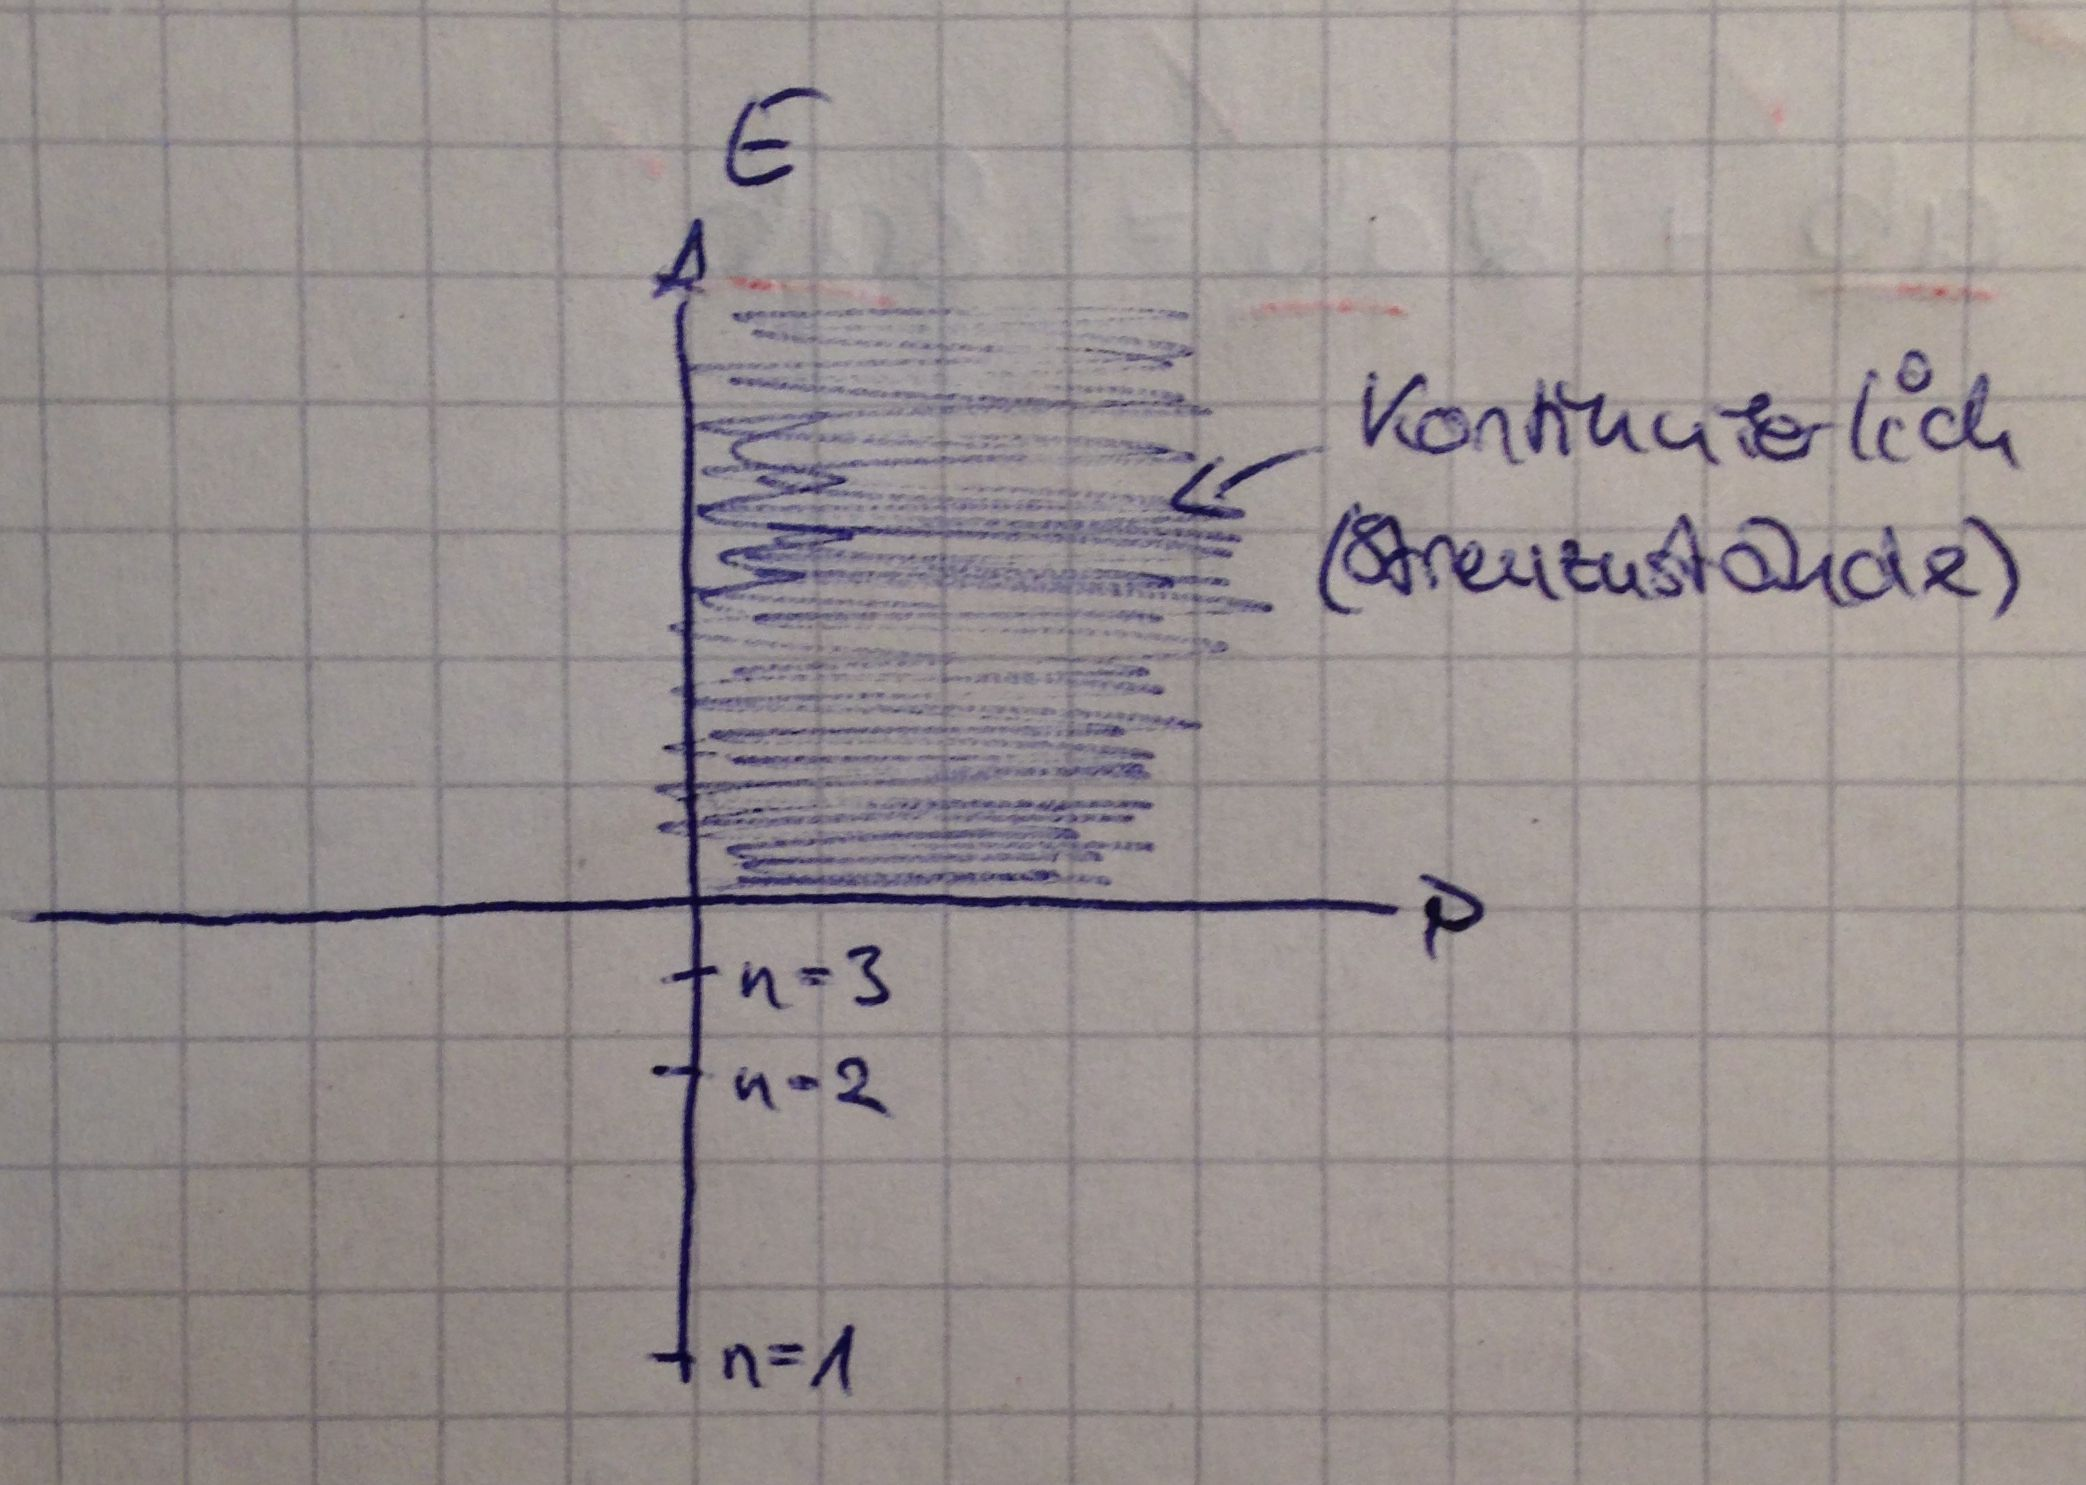
\includegraphics[width=10cm]{Ersatzgraph2.jpg}
		\end{center}
	\end{figure*}

	$P_{\alpha n}(t)$ ist Übergangswahrscheinlichkeits\underline{dichte}
	
	Übergangswahrscheinlichkeit: 
		\begin{equation*}
			\int_{\alpha_0}^{\alpha_1} \diff \alpha P_{\alpha n} (t)
		\end{equation*}
	Übergangsrate (Übergangswahrscheinlichkeit pro Zeiteinheit)
		\begin{align*}
			\underbrace{W_{\alpha \leftarrow n}}_{
				\mathclap{\text{Übergangsrate von~} n \text{~nach~} \alpha}}
			&= \int \diff \alpha \frac{P_{an}(t)}{t} \\
			&\underset{t \rightarrow \infty}{=} 
			\int \diff \alpha \frac{2 \pi}{\hbar^2} 
			\delta(\omega_\alpha - \omega_n) \left| \braket{m | H^1 | n}\right|^2 \\
			&= \int \diff \alpha \frac{2 \pi}{\hbar} 
			\delta (E_\alpha - E_n) \left| \braket{\alpha | H^1 | n}\right|^2
		\end{align*}
	(hier meinte Herr Prof. Bali mit einem Pfeil auf $E_\alpha$: Zeitunabhängige Störung erzwingt Energieerhaltung)
	
	Dichte von Zuständen:
		\begin{align*}
			\rho &= \int \diff \alpha \delta (E_\alpha - E)  \\
			\diff \alpha &= \rho(E_\alpha) \diff E_\alpha: \text{~Zahl der Zustände im ``Ìntervall''~} \diff E_\alpha
		\end{align*}
		\begin{align*}
			\boxed{
				W_{\alpha \leftarrow n} = \frac{2 \pi}{\hbar} \rho(E_n)
					\left| \braket{\alpha | H^1 | n}\right|^2
				}
			\text{~Fermis ``Goldene Regel'' (Wenzel)}
		\end{align*}
	Probleme bei 
		\begin{itemize}
			\item $t$ sehr groß $\Rightarrow \int \diff \alpha P_{\alpha n} > 1$.
			\item $t  << \frac{1}{|\omega_\alpha - \omega_n|}$ (keine $\delta$- Funktion)   
		\end{itemize}	
	Gültigkeitsbereich:
		\begin{itemize}
			\item $\Delta E$ Verteilung der Endzustände muss größer sein als die Breite von $\frac{\sin^2 (\frac{1}{2}(\omega_\alpha - \omega_n) t)}{(\omega_\alpha - \omega_n)^2}$. Damit $\delta$- Funktionsapproximation gerechtfertigt ist, muss $t \gg \frac{2 \alpha \pi}{\Delta E}$ (Version der Unschärferelation)
			\item $t$ muss klein genug sein, damit 1.Ordnung Störungstheorie gerechtfertigt ist:
			\\ $t \ll \frac{1}{W_{\alpha \leftarrow n}}$
		\end{itemize}
	\subsection{Periodische Störungen}
		\begin{align*}
			H^1(t) &= \left[H_\omega e^{-i \omega t} + H^\dagger_\omega e^{i \omega t}\right]
			\Theta(t) ,& \omega &> 0 \\
			H^{1 \dagger}(t) &= H^1(t) &\Rightarrow H^1(t) &= 0 \text{~für~} t < 0 
		\end{align*}
		\begin{align*}	
			c_m(t) - \delta_{mn} &= - \frac{i}{\hbar} \int_{0}^{t'} \diff t'
			\left\{ \braket{m | H_\omega | n} e^{i (\omega_m - \omega_n - \omega) t'} +
			\braket{m | H_\omega^\dagger | n} e^{i (\omega_m - \omega_n + \omega) t'}
			\right\} + \ldots \\
			\marginnote{Zitat Balis: jetzt bekommen wir hier viele Sinüsse. XD}
			&= - \frac{i}{\hbar} 
			\left\{ \braket{m | H_\omega | n} 
				\frac{\sin \left[\frac{1}{2} (\omega_m - \omega_n + \omega) t 
					\right]}{\frac{1}{2} (\omega_m - \omega_n + \omega)}
				e^{\frac{i}{2} (\omega_m - \omega_n - \omega) t} ~+ \right. \\
			&+ \left. \braket{m | H_\omega^\dagger | n}
				\frac{\sin \left[\frac{1}{2} (\omega_m - \omega_n - \omega) t 
					\right]}{\frac{1}{2} (\omega_m - \omega_n - \omega)}
				e^{\frac{i}{2} (\omega_m - \omega_n + \omega) t}	
			\right\} \\
		\end{align*}
		\begin{align*}
			\Rightarrow \left|c_m(t) - \delta_{mn}\right|^2 
			&= \frac{1}{\hbar^2} 
			\left\{ \left|\braket{m | H_\omega | n}\right|^2
				\frac{4 \sin^2 \left( \frac{1}{2} \left( \omega_{mn} - \omega\right) t
				\right)}{(\omega_{mn} - \omega)^2} ~+ \right. \\
			&+ \left. \left|\braket{m | H^\dagger_\omega | n}\right|^2
			\frac{4 \sin^2 \left( \frac{1}{2} \left( \omega_{mn} + \omega\right) t
				\right)}{(\omega_{mn} + \omega)^2}
			+ \text{gemischte Terme}
			\right\}
		\end{align*}
	mit $\omega_{mn} = \omega_m - \omega_n$
	
		\begin{figure*} [tbp]
			\begin{center}
				\includegraphics[width=10cm]{Ersatzgraph3.jpg}
			\end{center}
		\end{figure*}
	HIER GRAPH EINFÜGEN
	\FloatBarrier
		\begin{align*}
			\omega_m &= \omega_n + \omega &\Rightarrow E_m &= E_n + \hbar \omega: \text{Absorption} \\
			\omega_m &= \omega_n - \omega &\Rightarrow E_m &= E_n - \hbar \omega: \text{Emission}
		\end{align*}
		\underline{Goldene Regel:} für periodische Störung\marginpar{22.10.2015}
		\begin{align*} 
		W_{m \leftarrow n} &= 
		\frac{2 \pi}{\hbar} \rho (E_n + \hbar \omega) \left|\braket{m | H_\omega | n}\right|^2 &
		E_m &= E_m + \hbar \omega \text{~(Absorption)} \\
		W_{m \leftarrow n} &= 
		\frac{2 \pi}{\hbar} \rho (E_n - \hbar \omega) \left| \braket{m | H_\omega^\dagger | n}\right|^2 &
		E_m &= E_n - \hbar \omega \text{~(Emission)}
		\end{align*} \marginpar{bei dem 2ten braket fehlte das Betragsquadrat}
		Dichte
		\begin{align*}
		\rho (E) = \int \diff \alpha \delta(E_\alpha - E)
		\end{align*}
		für kontinuierliches Spektrum $\ket{m} \sim \ket{\alpha}$.
		
	\subsection{Absorpiton und Emission von elektromagnetischer Strahlung}
	Beispiel: Wasserstoffatom
		\begin{align*}
		e^- &: \text{Ladung~} q \\
		m &: \text{Masse}
		\end{align*}
		\begin{align*}
			H &= \frac{1}{2m} \left( \vec{p} + \frac{e}{c} \vec{A}' (\vec{r} , t)\right)^2
			- e \phi' (\vec{r} , t) 
			&\text{mit~} \vec{A}' &= \vec{A}_{\text{Proton}} + \underbrace{\vec{A} (\vec{r} , t)}_{\mathclap{\text{Photen von Welle}}}		
		\end{align*}
	$\vec{A}' (\vec{r} , t)$ und $\phi' (\vec{r} , t)$ sind Beiträge von elektromagnetischer Welle und vom Proton (statisch). \marginpar{das kann so auch nicht stimmen}
		\begin{align*}
			\phi' (\vec{r} , t) &= \underbrace{\frac{e}{4 \pi \hbar c}}_{\mathclap{\text{statisches Feld von Protonen}}}
			\frac{1}{r} + \phi (\vec{r} , t) \\
			H &= \underbrace{H^0}_{\mathclap{\text{ungestört von Wasserstoff-Atom (zeitunabh.)}}}
			+ \frac{e}{2 m c} \left( \vec{p} \vec{A} (\vec{r} , t) + \vec{A} (\vec{r} , t) \vec{p} + \frac{1 \cdot e^2}{2 m c^2} \vec{A}^2 (\vec{r} , t) - e\phi (\vec{r} , t) + \cdots 
			\right)
		\end{align*} 
	$e \vec{A}$ klein $\Rightarrow e^2 \vec{A}^2$ vernachlässigen \\
	$\Rightarrow$ Coulombeichung:
		\begin{itemize}
			\item $\vec{\nabla} \vec{A} = 0 \rightarrow \vec{p} \vec{A} = 0$ 
			\item $\phi (\vec{r}, t) = \text{const.} = 0$
		\end{itemize}
		\begin{equation*}
			\rightarrow H = H^0 +
			\underbrace{\frac{e}{2 m c} \vec{A} (\vec{r} , t) \vec{p}}_{\mathclap{\text{Störterm~} H^1(t)}} 
			= H^0 + H^1(t)
		\end{equation*}
	Man kann zeigen 
		\begin{equation*}
			\erw{\frac{\vec{p}}{m}} = \erw{\frac{i}{\hbar} \left[H^0 , \vec{r}\right]}
		\end{equation*}
	Nebenbedingung: Für Atome mit mehr als 1 $e^-$
		\begin{align*}
			\vec{p} &= \sum_i \vec{p}_i 
			&\rightarrow \erw{\frac{\vec{p}}{m}} &= \frac{i}{\hbar} \erw{\left[H^0 , \vec{R}\right]}
			&\text{mit~} \vec{R} &= \sum_i \vec{r}_i
		\end{align*}
	Betrachte elektromagnetische Welle
		\begin{align*}
			\vec{A}(\vec{r} , t) &= 
			\mathrm{Re} \left[ \vphantom{ \vec{A}_0 \vec{\epsilon} ~ e^{i(\vec{k} \vec{r} - \omega t)}} \right.
			\overbrace{\vec{A}_0}^{\mathclap{\in \mathds{C}}}
			~ \underbrace{\vec{\epsilon}}_{\mathclap{\mathds{R}^3 \text{-Polarisationsvektor mit~} |\vec{\epsilon}| = 1}}
			~ e^{i(\vec{k} \vec{r} - \omega t)}
			\left. \vphantom{ \vec{A}_0 \vec{\epsilon} ~ e^{i(\vec{k} \vec{r} - \omega t)}} \right] \\
			\vec{\epsilon} ~\vec{k} &= 0
		\end{align*}
	Dispersionsrelation: 
		\begin{equation*}
			\omega = |\vec{k}| c
		\end{equation*}
	Hinweis 
		\begin{align*}
			\partial_{t} &= \vec{E} \\
			\mathrm{rot} \vec{A} &= \vec{B}
		\end{align*}
	Intensität ists bestimmt durch $A_0^2$
		\begin{align*}
			\rightarrow I &= \overline{|\vec{S}|} & \text{zeitliches Mittel ist nötig da $\vec{S}$ fluktuiert!}
		\end{align*}
	$| \vec{S} |$ ist Pointing-Vektor 
		\begin{align*}
			| \vec{S} | &= c |\vec{E}| |\vec{B}| = c |E|^2 &\text{da~} |\vec{E}| &= |\vec{B}| \text{~ in Coulombeichung} \\
			\text{mit~} \vec{E} &= \frac{1}{c} \partial_t \vec{A} 
			&\rightarrow |\vec{S}| &= \frac{1}{c} \left|\partial_t \vec{A}\right|^2
		\end{align*}
	Somit ist die Intensität:
		\begin{align*}
			I &= \underbrace{\frac{\omega}{2 c}}_{\mathclap{\text{aus zeitlichem Mittel~} \int_{0}^{2 \pi} \diff \phi \frac{1}{2 \pi} \sin^2 \phi = \frac{1}{2}}}
			|A_0|^2
		\end{align*}
	Mittlere Energiedichte der elektromagnetischen Welle
		\begin{align*}
			u (\vec{r}) &=
			\frac{1}{2} \overline{\left( E^2(\vec{r} , t) + B^2(\vec{r} , t) \right)} 
			= \frac{1}{c} \overline{|\vec{S}|} = 
			\frac{I}{c} = \frac{\omega^2}{2 c^2} |A_0|^2 \\
			\overline{u} (\omega) &= \frac{\omega^2}{2 c^2} |A_0|^2
		\end{align*}
	Störoperator in Coulombeichung
		\begin{align*}
			H^1 &= \frac{e}{2 m c} \vec{A} (\vec{r} , t) \vec{p} \\
			&= \frac{e}{m c}
			\left[A_0 e^{i(\vec{k} \vec{r} - \omega t)} ~\vec{\epsilon}~\vec{p}
			+ A^*_0 e^{-i(\vec{k} \vec{r} - \omega t)} ~\vec{\epsilon}~\vec{p}
			\right] \\
			&+ \frac{e^2}{m c^2} \underbrace{|A_0|^2}_{\mathclap{\text{sehr klein~} \rightarrow \text{~wir vernachlässigen diesen}}} 
			\left(1 + \cos \left(2 (\vec{k} \vec{r} - \omega t)\right)\right) \\
			H^1 &= \underbrace{H_\omega}_{\mathclap{\frac{e}{m c} A_0 e^{i \vec{k} \vec{r}} \vec{\epsilon}~\vec{p}}} 
			e^{-i \omega t} 
			+ H_\omega^\dagger e^{i \omega t}
		\end{align*}
	Wir wollen nun $W_{m \leftarrow n}$ ausrechnen:
		\begin{align*}
			\left|\braket{m | \frac{e}{m c} A_0 e^{i \vec{k} \vec{r}} \vec{\epsilon}~\vec{p} |n}\right|^2
			= \frac{e^2}{m^2 c^2} |A_0|^2 \left| \braket{m | e^{i \vec{k} \vec{r}} \vec{\epsilon}~\vec{p} | n}\right|^2
		\end{align*}
	Übergangsrate: Absorption: $\omega_m > \omega_n$, $\omega_m = \omega_n + \omega$
		\begin{equation*}
			W_{m \leftarrow n} = 
			\frac{1}{t \hbar} \int \limits_{-\infty}^{\infty} 
			\diff E \rho_\omega (\omega) P_{nm} (t)
		\end{equation*}
	Wir machen $t$ groß $\Rightarrow$ Fermiregeln
		\begin{align*}
			\frac{2 \pi}{\hbar} \left|\braket{m | H_\omega | n}\right|^2 &\rho_\omega (\omega) \\
			&\rho_\omega (\omega) \text{~ist Dichte von Zuständen mit~} \omega = \frac{E}{\hbar} \\
			&\text{und~ }\rho_\omega (\omega)\sim \delta (\omega + \omega_{mn})
		\end{align*}
		\begin{align*}
			W_{m \leftarrow n} &= 
			\frac{4 \pi e^2}{m^2 \hbar^2 \omega_{mn}^2} u(\omega_{mn}) 
			\left|\braket{m | e^{i \vec{k} \vec{r}} (\vec{\epsilon} \cdot \vec{p}) | n}\right|^2 \\
			\erw{\hat{p}} &= \frac{i m}{\hbar} \left[H^0 , \vec{r} \right] 
		\end{align*}
		\begin{align*}
			\text{mit~}\alpha = \frac{e^2}{4 \pi \hbar c} :
			\boxed{W_{m \leftarrow n} = \frac{16 \pi^2 \alpha c}{\hbar^3 \omega_{mn}^2} 
				u (\omega_{mn}) \left|\braket{m | e^{i \vec{k} \vec{r}} \left[H^0 , \vec{r} \cdot \vec{\epsilon}\,\right] | n}\right|^2
			}
		\end{align*}
	Dipolnäherung: 
		\begin{equation*}
			e^{i \vec{k} \vec{r}} = 1 + 
			\underbrace{(i \vec{k} \vec{r})}_{\substack{\mathcal{O}(\alpha)}}
		\end{equation*}
	Der $\mathcal{O}(\alpha)$ Term kann vernachlässigt werden, denn:
		\begin{align*}
			\vec{k} \cdot \vec{r} 
			&\sim \frac{\omega}{c} n^2 a_B
			\sim \frac{\alpha \hbar c}{2 n^2 a_B} \frac{n^2 a_B}{\hbar c}
			\sim \frac{\alpha}{2} \\
			\alpha &\approx \frac{1}{137} \\
			n &: \text{Hauptquantenzahl} \\	
			a_B &: \text{Bohrscher Radius}		
		\end{align*}
	Jetzt wollen wir wissen was $\braket{m | \left[H^0 , \vec{r}\right] | n}$ ist
		\begin{align*}
			\vec{\epsilon} \braket{m | \left[H^0 , \vec{r}\right] | n} 
			= \hbar \overbrace{(\omega_m - \omega_n)}^{\mathclap{\omega_{mn}}} \vec{\epsilon} \braket{m | \vec{r} | n}
		\end{align*}
	Nebenbemerkung 
		\begin{align*}
			\bra{m} H^0 &= \bra{m} \hbar \omega_m \\
			-H \ket{n} &= -\hbar \omega_n \ket{n}
		\end{align*}
		\begin{empheq}[box=\boxed]{align*}
			\text{In Dipolnäherung:} \\
					W_{m \rightarrow n} &= \frac{16 \pi^2 \alpha c}{\hbar} u(\omega_{mn}) 
					\left|\braket{m | \vec{\epsilon} \cdot \vec{r} | n}\right|^2\\
					&= \frac{4 \pi}{\hbar^2} u(\omega_{mn}) 
					\left|\braket{m | \vec{\epsilon} \cdot \vec{d} | n}\right|^2\\
					&\text{mit Dipoloperator:~} \vec{d} = e \vec{r} = \sqrt{4 \pi \hbar c \alpha} \cdot \vec{r}
		\end{empheq}
		\begin{equation*}
			\braket{\vec{r} | n \ell m} = \psi_{n \ell m} (\vec{r}) 
			= \frac{u_{n \ell}(r)}{r} Y_{\ell m} (\Theta, \phi)
		\end{equation*}
	\underline{Dipolauswahlregeln:}
		\begin{align*}
			\braket{n' \ell' m' | \vec{r} | n \ell m} &\neq 0 \\
			&\Rightarrow \int \diff \Omega~Y^*_{\ell' m'}(\Omega)~\vec{r}~Y_{\ell m} (\Omega) \neq 0 \\
			\vec{r} &= \sqrt{\frac{4 \pi}{3}} r 
			\left( \vphantom{-\frac{1}{\sqrt{2}}} \right. 
				\frac{1}{\sqrt{2}} 
				\underbrace{(-Y_{1,1} + Y_{1,-1})}_{\mathclap{\sin \Theta \cos \phi}},
				\frac{1}{\sqrt{2}} \underbrace{(Y_{1,1} + Y_{1,-1})}_{\mathclap{\sin \Theta \sin \phi}},
				Y_{1,0}
			\left. \vphantom{-\frac{1}{\sqrt{2}}} \right) \\
			&= r \sum_{i,\lambda} \vec{e}_i d_{i,\lambda} Y_{1,\lambda} \\
			&\text{wobei~} i = \{x,y,z\} \text{~und~} \lambda \in \{-1,0,1\} 
		\end{align*}  
	(\textcolor{red}{sollte da nicht $\delta_{i \lambda}$ stehen statt $d_{i\lambda}$?})
		\begin{equation*}
			Y_{1,\lambda} Y_{\ell m} = c_- Y_{\ell - 1, m + \lambda}
			+ c_0 Y_{\ell, m+\lambda} + c_+ Y_{\ell + 1, m + \lambda}
		\end{equation*}
	mit $c_-,c_0, c_+$ Clebsch-Gordon Koeffizienten.
	
	Wir führen $m' = m + \lambda$ ein, weil 
		\begin{equation*}
			\int \diff \Omega ~Y^*_{\ell', m'} Y_{L, m+\lambda} = \delta_{\ell, L} \delta_{m', m+\lambda}
		\end{equation*}
		\begin{equation*}
			\Rightarrow \boxed{\Delta m = m' - m = 0, \pm 1}
		\end{equation*}
	Paritätsoperator:
		\begin{align*}
			\mathds{P} \vec{r} &= -\vec{r} & &\mathds{P} Y_{\ell m}(\Theta, \phi) = (-)^\ell Y_{\ell m}(\Theta, \phi) \\
%		\end{align*}
%		\begin{align*}
			&\int \diff \Omega~Y_{\ell' m'}(\Omega)~\vec{r}~Y_{\ell m} (\Omega) =
			& &\text{analog zu:} \\ 
			&= \int \diff \Omega ~\mathds{P} \left(~Y^*_{\ell' m'}(\Omega)
			~\vec{r}~Y_{\ell m}(\Omega)\right)& 
			&\int\limits_{-\infty}^{\infty} \diff x f(x) 
			= \int\limits_{-\infty}^{\infty} \diff x f(-x) \\
			&= \int \diff \omega (-)^{\ell'} (-1) (-)^\ell
			\left( Y_{\ell'm'}(\Omega) ~\vec{r}~ Y_{\ell m}(\Omega)\right) \\
			&= (-)^{\ell + \ell' + 1} \int \diff \Omega ~Y_{\ell' m'}(\Omega)~\vec{r}~Y_{\ell m} (\Omega)
		\end{align*}
	Integral $\neq 0 \Rightarrow 1= (-)^{\ell + \ell' + 1} \Rightarrow \ell + \ell'$ ungerade \\
	Und dies gilt nur für $\ell' = \ell, \ell+1, \ell-1$
		\begin{empheq}[box=\boxed]{align*}
			\Rightarrow
			\Delta \ell = \ell' + \ell &= \pm 1 &\text{für~} \ell &\geq 1 \\
			&= 1 &\text{für~} \ell &= 0
		\end{empheq}
	$\Delta m = 0$ tritt nur für $\braket{\ell' , m' | z | \ell, m}$ auf \marginpar{was zur Hölle ist z?}
	
	Betrachte inkohärente Überlagerung von elektromagnetischen Wellen (keine Polarisation):
		\begin{align*}
			\frac{1}{4 \pi} \int 
			\underbrace{\diff \Omega_{\vec{\epsilon}}}_{\mathclap{\text{Mittel über alle~} \vec{\epsilon}}} 
			\left|\braket{m | \vec{d} \cdot \vec{\epsilon} | n}\right|^2 
			&= \frac{1}{4 \pi} \int \diff \Omega_{\vec{\epsilon}} 
			\braket{m | \vec{d} \cdot \vec{\epsilon} | n} \braket{n | \vec{d} \cdot \vec{\epsilon} | m} \\
			&= \sum_{i,j} \braket{m | d_i | n} \braket{n | d_j | m} 
			\frac{1}{4 \pi} \int \diff \Omega_{\vec{\epsilon}} 
			\overbrace{\epsilon_i \epsilon_j}^{\mathclap{\delta_{ij}\frac{\epsilon^2}{3}}} \\
			&= \frac{4 \pi}{3} \left|\braket{m | \vec{d} | n}\right|^2
		\end{align*} 
		\begin{empheq}[box=\boxed]{align*}
			W_{m \leftarrow n} &= 
			\frac{4 \pi}{3 \hbar^2} u (\omega_{mn}) 
			\left| \braket{n | \vec{d} | m}\right|^2 
			&\text{mit~} \vec{d} &= e \vec{r} \text{~Dipolmoment}
		\end{empheq}
		\marginpar{26.10.2015} Okay, Leute. Herr Prof. Bali hat heute eine Seite Korrektur an die Tafel geschrieben, aber ich weiß nicht wo jetzt welche 2 weg oder hin muss, denn am Ende wusste er es selbst auch nicht mehr. Deshalb schreibe ich einfach das auf, was ich mitgeschreiben habe. 
		
		Korrektur ! 
		\begin{align*}
		\vec{A} (\vec{r} , t) &=
		2 \mathrm{Re} \left(
		A_0 \vec{\epsilon} e^{i (\vec{k} \vec{r} - \omega t)}
		\right) \\
		|\vec{S}| &=
		c |\vec{E}| = \frac{\omega^2}{c} 4 |A_0|^2 \\
		u &= \frac{1}{2} \overline{\left( \vec{E}^2 + \vec{B}^2 \right)} 
		= \frac{1}{c} \overline{|\vec{S}|} 
		= \frac{\omega^2}{c^2} 2 |A_0|^2 = \frac{I}{c} \\
		H^1 &= \frac{e}{mc} \left[
		A_0 e^{i (\vec{k} \vec{r} - \omega t)} \vec{\epsilon} \,\vec{p} 
		+ A_0^\dagger e^{-i (\vec{k} \vec{r} - \omega t)} \vec{\epsilon} \,\vec{p}
		\right] \\
		&+ \frac{e^2}{m c^2} 4 |A_0|^2 \left( 1 + \cos (2 (\vec{k} \vec{r} - \omega t))\right) \\
		| \braket{m | H_\omega | n} |^2 &=	
		\frac{e^2}{4\!\!\!/ m^2 c^2} |A_0|^2
		| \braket{m | e^{i \vec{k} \vec{r}} \vec{\epsilon} \,\vec{p} | n} |^2 
		= \frac{e^2 u(\omega)}{2 m^2 \omega^2} 
		| \braket{m | e^{i \vec{k} \vec{r}} \vec{\epsilon} \,\vec{p} | n} |^2 \\
		W_{m \leftarrow n} &= \frac{4\!\!\!/ \pi e^2 u(\omega_{mn})}{m^2 \hbar^2 \omega_{mn}^2}
		|\braket{\ldots}|^2
		\end{align*}
		\begin{empheq}[box=\boxed]{align*}
		W_{m \leftarrow n} &=
		\frac{4 \pi^2 \alpha c}{\hbar^3 \omega_{mn}} u(\omega_{mn}) 
		| \braket{m | e^{i \vec{k} \vec{r}} \left[ H^0, \vec{r} \cdot \vec{\epsilon} \, \right]} |^2
		\end{empheq}
		Dipolnäherung:
		\begin{align*}
		W_{m \leftarrow n} &=
		\frac{4 \pi^2 \alpha c}{\hbar} u(\omega_{mn}) 
		| \braket{m | \vec{\epsilon} \cdot \vec{r} | n} |^2 
		= \frac{\pi}{\hbar^2} u(\omega_{mn}) 
		| \braket{m | \vec{\epsilon} \cdot \vec{d} \,| n} |^2
		\end{align*}
		\begin{align*}
		\int \diff \Omega_\epsilon \epsilon_i \epsilon_j &= c \delta_{ij} \\
		\text{Beispiel: ~} \epsilon_z &= \cos \Theta \\
		\int \diff \Omega_\epsilon \epsilon_z^2 &= 
		\int_{0}^{2 \pi} \diff \phi \int_{-1}^{1} \diff (\cos \Theta) \cos^2 \Theta 
		= 2 \pi \left. \frac{\cos^3 \Theta}{3} \right|_{-1}^1 = \frac{4 \pi}{3} \\
		\Rightarrow c &= \frac{4 \pi}{3} 
		\end{align*}
		\begin{empheq}[box=\boxed]{align*}
		W_{m \leftarrow n} = \frac{\pi}{3 \hbar^2} u(\omega_{mn})
		| \braket{n | \vec{d} | m} |^2
		\end{empheq}
		\begin{figure*} [h]
			\begin{center}
				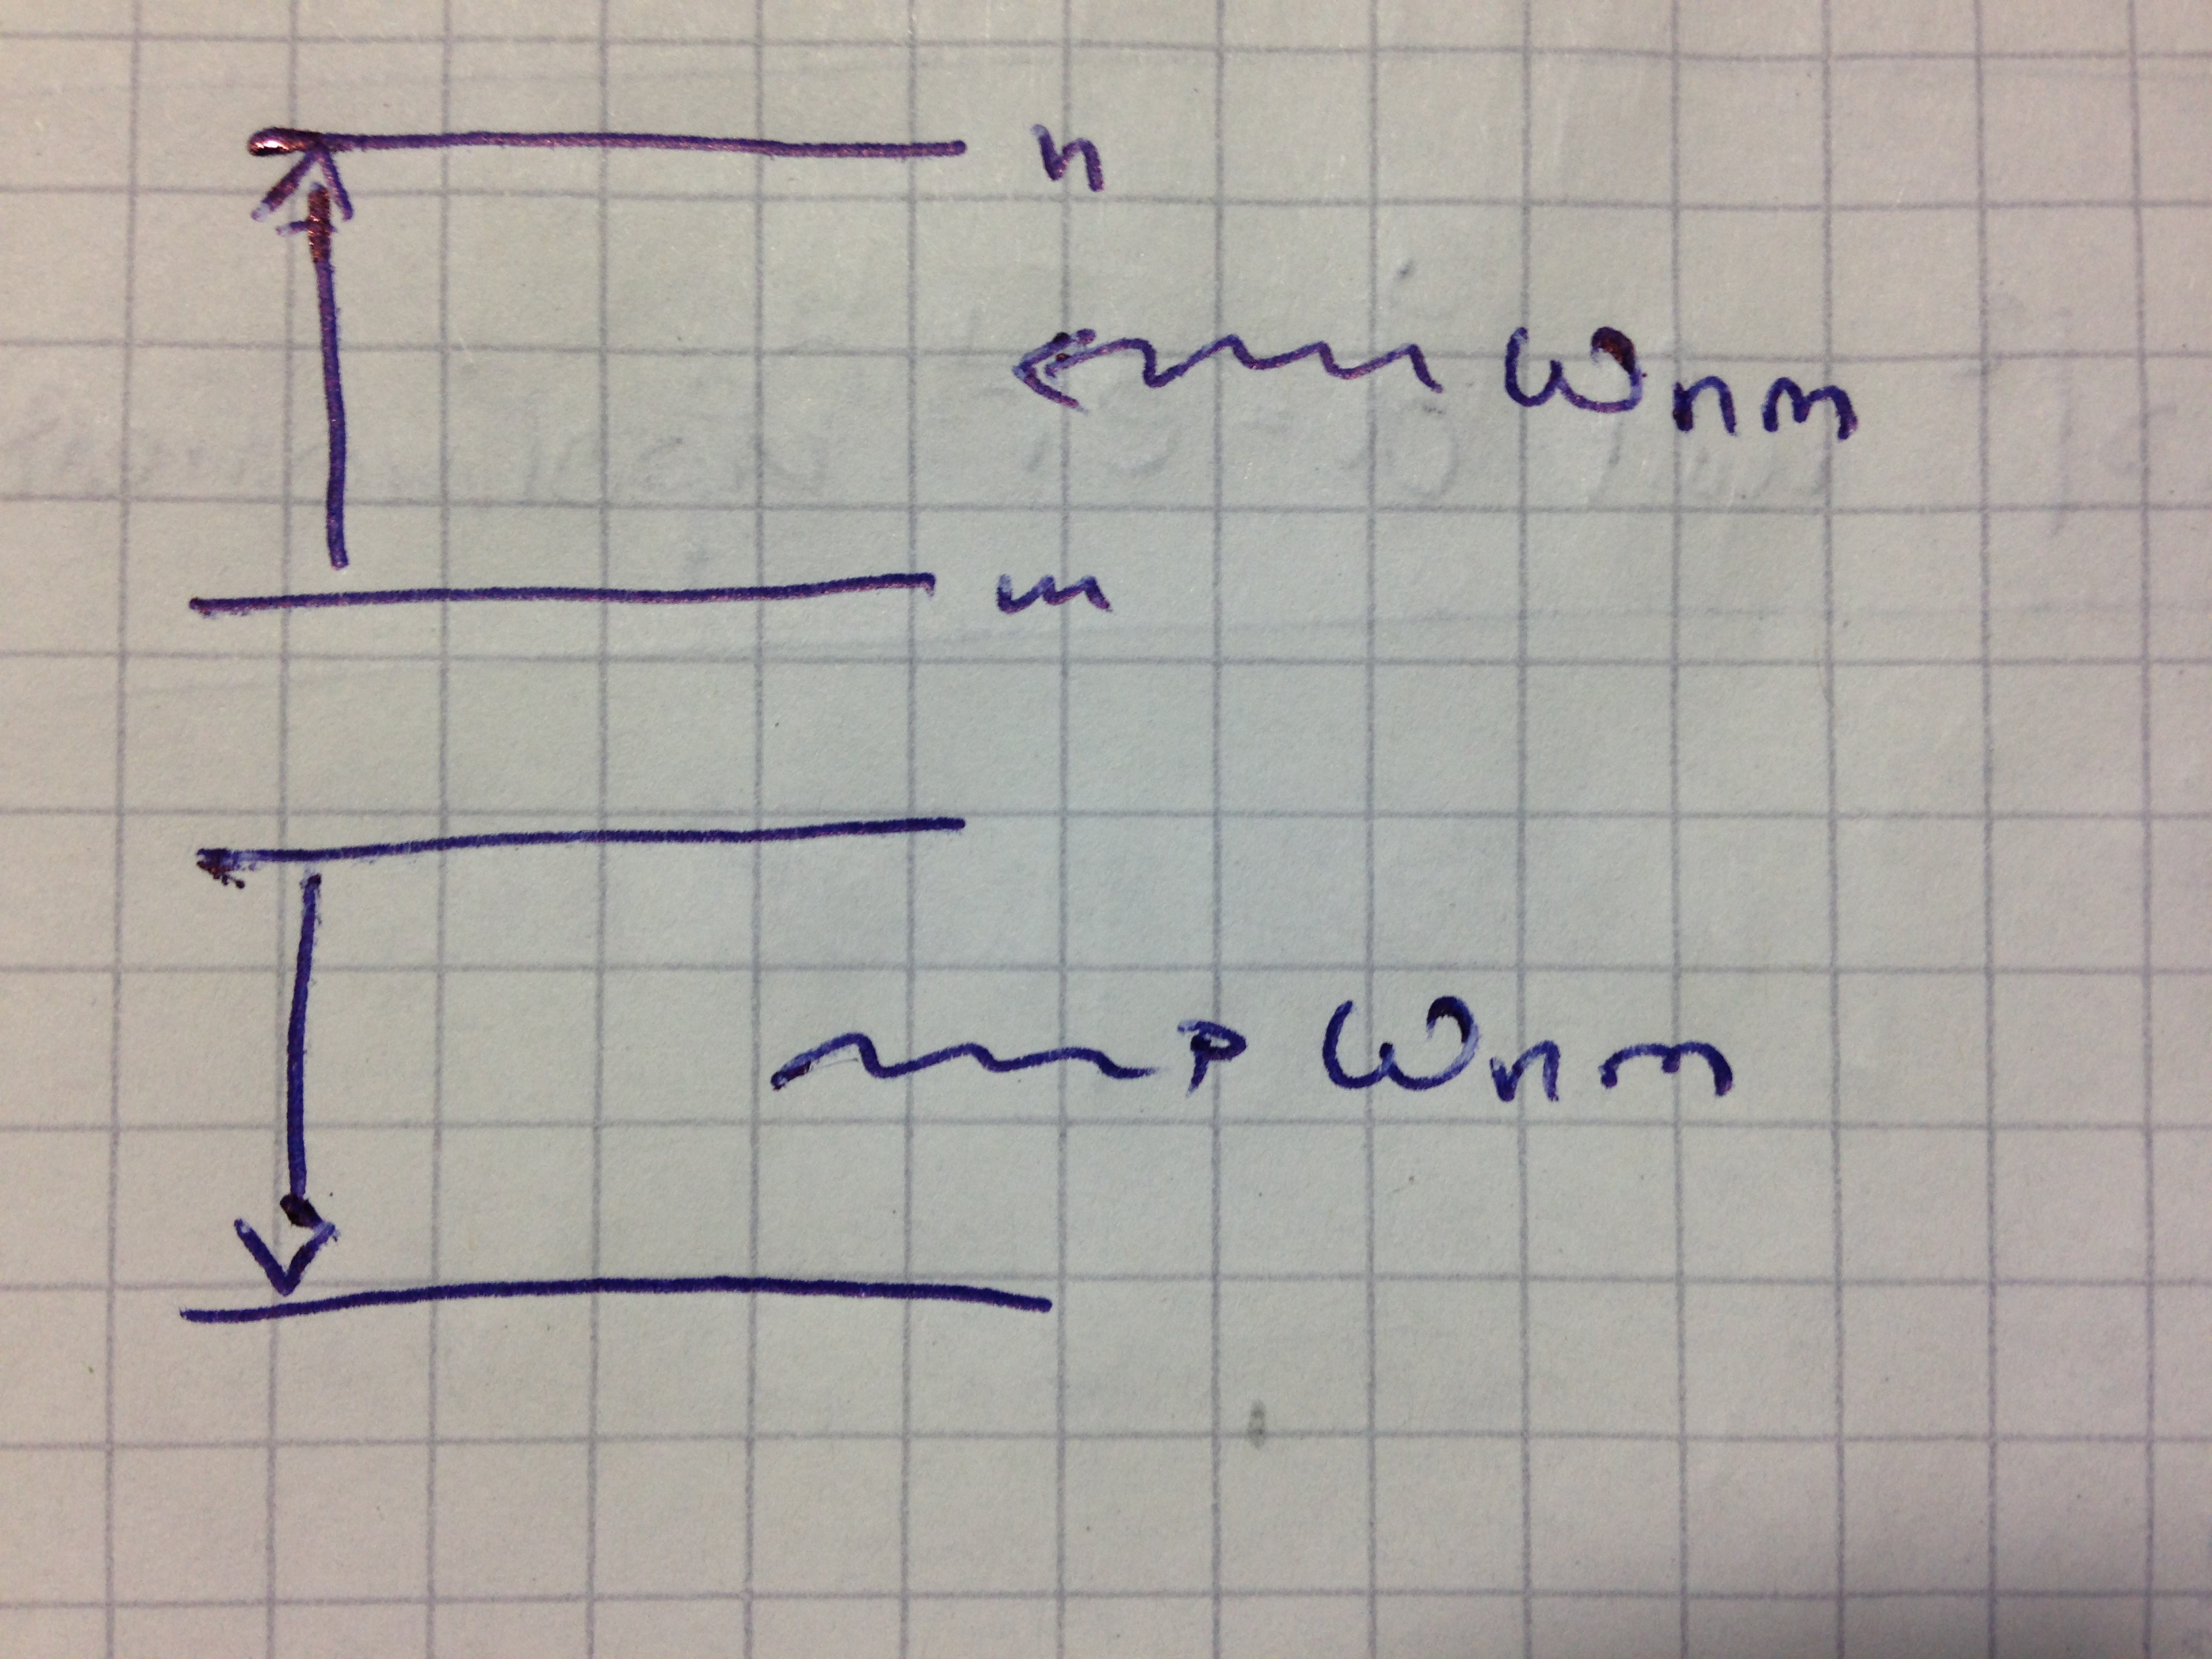
\includegraphics[width=10cm]{Bild1.jpg}
			\end{center}
		\end{figure*}
		\FloatBarrier
	\subsection{Spontane Emissions}
	Ein genaues Verständnis dieses Phänomens erfordert eine Quantentheorie des elektromagnetischen Feldes, die man Quantenelektrodynamik (QED) nennt. 
	\\
		
	Betrachte Kasten des Volumens $V = L^3$ \\	
	(Nebenbemerkung: Bei $L \rightarrow \infty$ gibt es infratrot ``Probleme'')
		\begin{align*}
			\vec{A} (\vec{r} , t) &= \vec{\epsilon}~ e^{i (\vec{k} \vec{r} - \omega_k t)} 
			,& \omega_k &= |\vec{k}| \cdot c 
		\end{align*}
	2 orthogonale Polarisationsrichtungen: 
		\begin{align*}
			\vec{\epsilon}_+ \cdot \vec{\epsilon}_- &= 0 
			,& &\vec{k} \cdot \vec{\epsilon}_\pm = 0 \\
			& & &(\text{transversale Welle~} \vec{\nabla} \vec{A} = 0 )
 		\end{align*}
 		\begin{align*}
	 		\vec{\epsilon}_\lambda ~,~ \lambda &\in \{ - , + \} \\
	 		\vec{A} (\vec{r} + L \vec{e}_x , t) &= \vec{A} (\vec{r} , t) &
	 		&\text{für periodische (nicht wichtig) Randbedingungen.} \\
	 		\Rightarrow \vec{k} L \vec{e}_x &= k_x L = 2 \pi n_x &
	 		&\left( e^{i \vec{k} \vec{r}} = e^{i \vec{k} (\vec{r} + L \vec{e}_x)} \right) \\
	 		n_x &\in \mathds{Z}. \\
	 		\vec{k} &= \frac{2 \pi}{L} \vec{n} ,& &n_x, n_y, n_z \in \mathds{Z}
 		\end{align*}
 	Allgemeines
	 	\begin{align*}
		 	\vec{A} (\vec{r} , t) = \frac{c}{\sqrt{2 V}}
		 	\sum_{\vec{k}} \sum_{\lambda \in \{+ , - \} }
		 	\vec{\epsilon}_\lambda (\vec{k}) 
		 	\underbrace{q_\lambda}_{\mathclap{\in \mathds{C}}} (\vec{k} , t) 
		 	e^{-i \vec{k} \vec{r}}
	 	\end{align*}
	Wir fordern $\vec{A} \in \mathds{R}^3$.
		\begin{align*}
			\Rightarrow q_\lambda (- \vec{k} , t) &= q^*_\lambda (\vec{k} , t) ,&
			&\vec{\epsilon}_\lambda (-\vec{k}) = \vec{\epsilon}_\lambda (\vec{k}) \\
			\text{Zusätzlich:~} q_\lambda (\vec{0} , t) &= 0 .& 
			&\text{(nur ebene Wellen)}
		\end{align*}
	Wellengleichung: 
		\begin{align*}
			\left(
				\vec{\nabla}^2 - \frac{1}{c^2} \frac{\partial^2}{\partial t^2} 
			\right)
			\vec{A} (\vec{r} , t) &= \overbrace{0}^{\mathclap{\text{im Vakuum}}} \\
			\overset{\text{Koeff.-Vergleich}}{\Rightarrow} 
			\frac{1}{c^2} \ddot{q}_\lambda (\vec{k} , t) + \vec{k}^2 q_\lambda &= 0
		\end{align*}
		\begin{align*}
			\boxed{\ddot{q}_\lambda (\vec{k} , t) + \omega_k^2 ~q_\lambda (\vec{k} , t)} = 0
		\end{align*}
	$q_\lambda$: Lösungen des harmonischen Oszillators mit Frequenz $\omega_k$. \\
	Energie des elektromagnetischen Feldes: 
		\begin{align*}
			E &= \int_V \diff^3 r ~u (\vec{r} , t) \\
			&= \int_V \diff^3 r \frac{1}{2} \left( \vec{E}^2 (\vec{r} , t) \vec{B}^2 (\vec{r} , t)
			\right) \\
			&= \frac{1}{2} \int_V \diff^3 r \left[
				\left(\frac{1}{c^2} \frac{\partial \vec{A}}{\partial t}\right)^2
				+ \left( \vec{\nabla} \times \vec{A}\right)^2
			\right] \\
			\left( \vec{\nabla} \times \vec{A}\right)^2 &=
			\vec{\nabla} \left(\vec{A} \times \left( \vec{\nabla} \times \vec{A} \right)\right)
			+ \left(\vec{A} \cdot \vec{\nabla}\right) 
			\underbrace{\left( \vec{\nabla} \cdot \vec{A}\right)}_{\mathclap{=0 \text{~(Coulombeichung)}}}
			- \vec{A} \cdot \vec{\nabla}^2 \cdot \vec{A} \\
			\text{zu der Klammer~} &\text{mit mehreren Rotationen:~} \\
			\int_V \diff^3 r~ \vec{\nabla} (\ldots) 
			&= \int_{\partial V} \diff^2 r~ \vec{n} (\vec{r}) (\ldots) = 0
		\end{align*}
		\begin{align*}
			\boxed{
				E = \frac{1}{2} \int \diff^3 r \left[ 
				\left(\frac{1}{c} \frac{\partial \vec{A}}{\partial t}\right)^2
				- \vec{A}~ \vec{\nabla}^2 \vec{A}
				\right]	
			}
		\end{align*}
	Nebenrechnung:
		\begin{align*}
			\int \diff^3 r (\dot{\vec{A}})^2 &= 
			\frac{c^2}{2 V} \sum_{\vec{k}, \lambda} \sum_{\vec{k}', \lambda'}
			\underbrace{\int \diff^3 r e^{i (\vec{k} + \vec{k}') \vec{r}}}_{
				\substack{V \delta_{\vec{k}, -\vec{k}} 
					\text{~für diskretes~} \vec{k},\\ 
					(2 \pi)^3 \delta^{(3)} (\vec{k} + \vec{k}') \\ 
					\text{~kontinuierliches~} \vec{k}}
				}
			\vec{\epsilon}_\lambda(\vec{k}) ~\vec{\epsilon}_{\lambda'} (\vec{k}')
			~\dot{q}_\lambda (\vec{k} , t) ~\dot{q}_{\lambda'} (\vec{k}' , t) 
			\\
			&\overset{\vec{k}' = -\vec{k}'}{=} 
			\frac{c^2}{2} \sum_{\vec{k}, \lambda, \lambda'}
			\vec{\epsilon}_\lambda (\vec{k}) ~\vec{\epsilon}_{\lambda'}(-\vec{k})~
			\dot{q}_\lambda (\vec{k} , t) ~\dot{q}_{\lambda'} (\vec{-k} , t)
			\\
			&= \frac{c^2}{2} \sum_{\vec{k}, \lambda, \lambda'}
			\vec{\epsilon}_\lambda (\vec{k}) ~\vec{\epsilon}_{\lambda'}(-\vec{k})~
			\dot{q}_\lambda (\vec{k} , t) ~\dot{q}^*_{\lambda'} (\vec{k} , t)
			\\
			&= \frac{c^2}{2} \sum_{\vec{k}} \sum_{\lambda \in \{+ , - \} }
			| \dot{q}_\lambda(\vec{k} , t)  |^2
		\end{align*}
	Analog:
		\begin{align*}
			\int_V \diff^3 r \left(- \vec{A} \vec{\nabla}^2 \vec{A}\right)
			&\overset{\text{part. Int.}}{=} \int_V \diff^3 r \left( \vec{\nabla} \vec{A} \right)^2 \\
			&= \frac{c^2}{2} \sum_{\vec{k}} \sum_{\lambda \in \{+ , - \} }
			\vec{k}^2 |q_\lambda (\vec{k} , t)|^2 \\
			E &= \frac{1}{4} \sum_{\vec{k} , \lambda} \left[
				|\dot{q}_\lambda (\vec{k} , t)|^2 + \omega^2_k |q_\lambda (\vec{k} , t)|^2
			\right] \\
			\text{wobei~} |\dot{q}_\lambda (\vec{k} , t)|^2 &= 
			\dot{q}_{1 \lambda}^2 (\vec{k} , t) + \dot{q}_{2 \lambda}^2 (\vec{k} , t) 
			\\
			\text{und~} 
			q_\lambda (\vec{k} , t) &= q_{1 \lambda} (\vec{k} , t) + i q_{2 \lambda} (\vec{k} , t) 
			,& q_{i \lambda} (\vec{k} , t) &\in \mathds{R} 
			\\
			q_\lambda (-\vec{k} , t) &= q_\lambda^* (\vec{k} , t) 
			&\Rightarrow q_{1 \lambda} (-\vec{k} , t) &= q_{1 \lambda} (\vec{k} , t) 
			\\
			& & q_{2 \lambda} (-\vec{k} , t) &= - q_{2 \lambda} (\vec{k} , t)			
		\end{align*}
		\begin{align*}
			E = \frac{1}{2} \sum_{\vec{k} \in H, \lambda}
			\left[
				\dot{q}_{1 \lambda}^2 (\vec{k} , t)
				+ \omega_k^2 ~q_{1 \lambda}^2 (\vec{k} , t)
				+ \dot{q}_{2 \lambda}^2 (\vec{k} , t)
				+ \omega_k^2 ~q_{2 \lambda}^2 (\vec{k} , t)
			\right]
		\end{align*}
	$\vec{k} \in H$ bedeutet $\vec{k}$ ist im Halbraum. z.B. $k_z > 0$
		\begin{align*}
			\text{für~} k_z &= 0 : k_y > 0 \\
			\text{für~} k_z &= k_y = 0 : k_x > 0 
		\end{align*}
	Zu jedem Wellenvektor $\vec{k} \in$ Halbraum und Polarisation $\lambda$ gehören je 2 harmonische Oszillatoren.	
		\begin{align*}
			H_{\text{harm.Oszil.}} &= 
			\frac{p^2}{2 m} + \frac{1}{2} m \omega^2 q^2 \\
			&= \frac{p^2}{2} + \frac{\omega^2}{2} q^2 
			&\text{für~} m &= 1 \text{~ist~} p = \dot{q} \\
			p_{i \lambda} (\vec{k}) \coloneqq \dot{q}_{i \lambda} \\
 		\end{align*}
 	für festes t gilt dann: 
	 	\begin{align*}
	 		H = \frac{1}{2} \sum_{\vec{k} \in H, \lambda}
	 		\left[
		 		p_{1 \lambda}^2 (\vec{k})
		 		+ \omega_k^2 ~q_{1 \lambda}^2 (\vec{k})
		 		+ p_{2 \lambda}^2 (\vec{k})
		 		+ \omega_k^2 ~q_{2 \lambda}^2 (\vec{k})
	 		\right]
	 	\end{align*}
	``quantisiere'' $H$ : $p \mapsto \hat{p} , q \mapsto \hat{q}$
		\begin{align*}
			\left.
			\begin{aligned}
			\left[ \hat{p}_{i \lambda} (\vec{k}) , \hat{q}_{j \lambda'} (\vec{k}')
			\right]
			&= -i\hbar \delta_{ij} \delta_{\lambda \lambda'} \delta_{\vec{k} \vec{k}'} \mathds{1}
			\\
			a_{i \lambda}(\vec{k}) 
			&= \sqrt{\frac{\omega_k}{2 \hbar}} 
			\left(\hat{q}_{i \lambda} (\vec{k}) + \frac{i}{\omega_k} \hat{p}_{i \lambda} (\vec{k})\right)
			\\
			a^\dagger_{i \lambda}(\vec{k})
			&= \sqrt{\frac{\omega_k}{2 \hbar}}
			\left(\hat{q}_{i \lambda} (\vec{k}) - \frac{i}{\omega_k} \hat{p}_{i \lambda} (\vec{k})\right)
			\end{aligned}
			\right\}
			\left[ a_{i \lambda} (\vec{k}) , a_{j \lambda'}^\dagger (\vec{k}')
			\right] 
			= \delta_{ij} \delta_{\lambda \lambda'} \delta_{\vec{k} \vec{k}'} \mathds{1}
		\end{align*}
		\begin{align*}
			\left.
			\begin{aligned}
				a_\lambda (\vec{k}) 
				&\coloneqq \frac{1}{\sqrt{2}} 
				\left(a_{1 \lambda} (\vec{k}) + i a_{2 \lambda} (\vec{k}) \right) \\
				a_\lambda (-\vec{k}) 
				&\coloneqq \frac{1}{\sqrt{2}} 
				\left(a_{1 \lambda} (\vec{k}) - i a_{2 \lambda} (\vec{k}) \right)
			\end{aligned}
			\right\}
			\Rightarrow 
			\begin{aligned}
				&a_\lambda (\vec{k}) \text{~für alle~} \vec{k} \\
				&\vec{k} \in H ~,~ -\vec{k} \in H
			\end{aligned}
		\end{align*}
	Rechnung:
		\begin{equation*}
			\left[
				a_\lambda (\vec{k}), a_{\lambda'}^\dagger (\vec{k}')
			\right]
			= \delta_{\lambda \lambda'} \delta_{\vec{k} \vec{k}'} \mathds{1}
		\end{equation*}
	Einsetzen (Rechnung)
		\begin{align*}
			\vec{A} (\vec{r}) &= 
			\sqrt{\frac{\hbar c^2}{2 V}} \sum_{\vec{k}, \lambda} \frac{1}{\sqrt{\omega_k}}
			\vec{\epsilon}_\lambda (\vec{k}) 
			\left\{ a_\lambda (\vec{k}) e^{i \vec{k} \vec{r}} 
			+ a^\dagger_\lambda (\vec{k}) e^{-i \vec{k} \vec{r}} 
			\right\}
			\\
			H &= 
			\sum_{\vec{k} , \lambda} \hbar \omega_k
			\left( a^\dagger_\lambda (\vec{k}) ~a_\lambda (\vec{k}) + \frac{1}{2}
			\right) & &\text{Problem?}
		\end{align*}
	Energien sind nur bis auf additive Konstante festgelegt. \\
	$E \mapsto E-E_0 ~,~ H \mapsto H - H_0 :$ Term $\frac{\hbar \omega_k}{2}$ hebt sich weg.
	
	Subtraktion der Nullpunktsenergie:
		\begin{align*}
			\boxed{ 
				H \coloneqq 
				\sum_{\vec{k}, \lambda} \left( a^\dagger_\lambda (\vec{k}) ~a_\lambda (\vec{k})\right)
				\hbar \omega_k
			}
		\end{align*}
		\begin{align*}
			H \ket{0} &= \ket{0} ,& 
			H\ket{\vec{k}, \lambda} &= 
			\hbar \omega_k \ket{\overbrace{\vec{k}}^{\mathclap{\text{Photon/Lichtquant}}} , \lambda}
		\end{align*}
	Poyntingvektor
		\begin{equation*}
			\vec{S} = c \vec{E} \times \vec{B}
		\end{equation*}
	Impuls
		\begin{align*}
			\vec{p} &= \int \diff^3 r \underbrace{\vec{S}}_{\mathclap{\text{Impulsdichte}}} 
			= c \int \diff^3 r 
			\left( - \frac{1}{c} \hat{\dot{\vec{A}}} \times (\vec{\nabla} \times \hat{\vec{A}})
			\right) \\
			&\overset{\text{Rechnung}}{=} 
			\sum_{\vec{k} , \lambda} \hbar \vec{k} ~a^\dagger_\lambda (\vec{k}) ~a_\lambda (\vec{k})
		\end{align*}
		\begin{empheq}[box=\boxed]{align*}
			\vec{p} \ket{\vec{k} , \lambda} = \hbar \vec{k} \ket{\vec{k} , \lambda}
		\end{empheq}
		Beim letzten Mal hatten wir $\vec{A} (\vec{r}, t)$ quantisiert wie folgt:\marginpar{29.10.2015}
		\begin{align*}
		\hat{\vec{A}} (\vec{r})= \sqrt{\frac{\hbar}{2V}} ~c
		\sum_{\vec{k}, \lambda \in \{+ , i\}}
		\frac{1}{\sqrt{\omega_k}} \vec{\epsilon}_\lambda (\vec{k}) 
		\left\{ a_\lambda (\vec{k}) e^{i \vec{k} \vec{r}}
		+ a^\dagger_\lambda (\vec{k}) e^{-i \vec{k} \vec{r}}
		\right\}
		\end{align*}
		Wobei
		\begin{align*}
		a^\dagger_\lambda (\vec{k}) \ket{0} 
		&= \overbrace{\ket{\lambda, \vec{k}}}^{\mathclap{\text{Photon}}} \\
		a_\lambda (\vec{k}) \ket{0} &= 0 \\
		\vec{\epsilon}_\lambda (\vec{k}) &: \text{Polarisation} \\
		\hat{\vec{A}} (\vec{r}) &: \text{Operator (keine gewöhnliche Welle)} \\
		\hat{\vec{A}} (\vec{r}) \ket{0} &= \vec{A} (\vec{r})\ket{0} 
		\end{align*}
		D.h $\vec{A} (\vec{r})$ ist ein Eigenwert und enthält keine $a$ oder $a^\dagger$.
		\begin{empheq}[box=\boxed]{align*}
		H = \sum_{\vec{k}, \lambda} \hbar \omega_k
		\underbrace{a^\dagger_\lambda (\vec{k})~a_\lambda (\vec{k})}_{\substack{\text{Nummern oder} \\ \text{Teilchenoperator}}}
		\end{empheq}
		Wobei $\omega_k = c |\vec{k}|$ und kein $\frac{1}{2} \hbar \omega$ vorhanden ist, was damit zutun hat, dass wir nur den Grundzustand betrachten (glaube ich \^{}\^{}).
		
		Auf jeden Fall gilt für $n=1$:
		\begin{align*}
		H \ket{\lambda, \vec{k}} &= \hbar \omega_k \ket{\lambda , \vec{k}} \\
		\hat{\vec{p}} &= \hbar \vec{k} \ket{\lambda , \vec{k}} \\
		E = |\vec{p}| c &\curvearrowright H = |\hat{p}| c \\
		H \ket{0} (&= E_0 \ket{0} = 0 \ket{0} ) = 0
		\end{align*}
		Unendliches Volumen: 
		\begin{align*}
		\frac{1}{V} \sum_{\vec{k}} &\longmapsto \int \frac{\diff^3 k}{(2 \pi)^3}
		& \text{Wobei das~} \vec{k} \text{~so aufgebaut ist:~}k_i &= n_i \frac{2 \pi}{L}, n_i \in \mathds{Z}
		\end{align*} \marginpar{Bleibt die Frage, was $n_i$ sind}
		\begin{align*}
		V \delta_{\vec{k} , 0} &\longmapsto (2 \pi)^2 \delta^{(3)} (\vec{k}) \\
		a_\lambda (\vec{k}) &\longmapsto \frac{1}{\sqrt{\lambda}} 
		& &\text{(wegen Infrarot cutoff)}
		\end{align*} \marginpar{kA was das genau ist}
		\begin{align*}
		\vec{A} (\vec{r}) =
		\sqrt{\hbar} \int \frac{\diff^3 k}{(2 \pi)^3} \frac{c}{\sqrt{2 \omega_k}}
		\sum_\lambda \vec{\epsilon}_\lambda (\vec{k})
		\left\{ a_\lambda (\vec{k}) e^{i \vec{k} \vec{r}}
		+ a^\dagger_\lambda (\vec{k}) e^{-i \vec{k} \vec{r}}
		\right\}
		\end{align*}
		Wir betrachten ab jetzt den Fall: 
		\begin{figure*} [ht]
			\begin{center}
				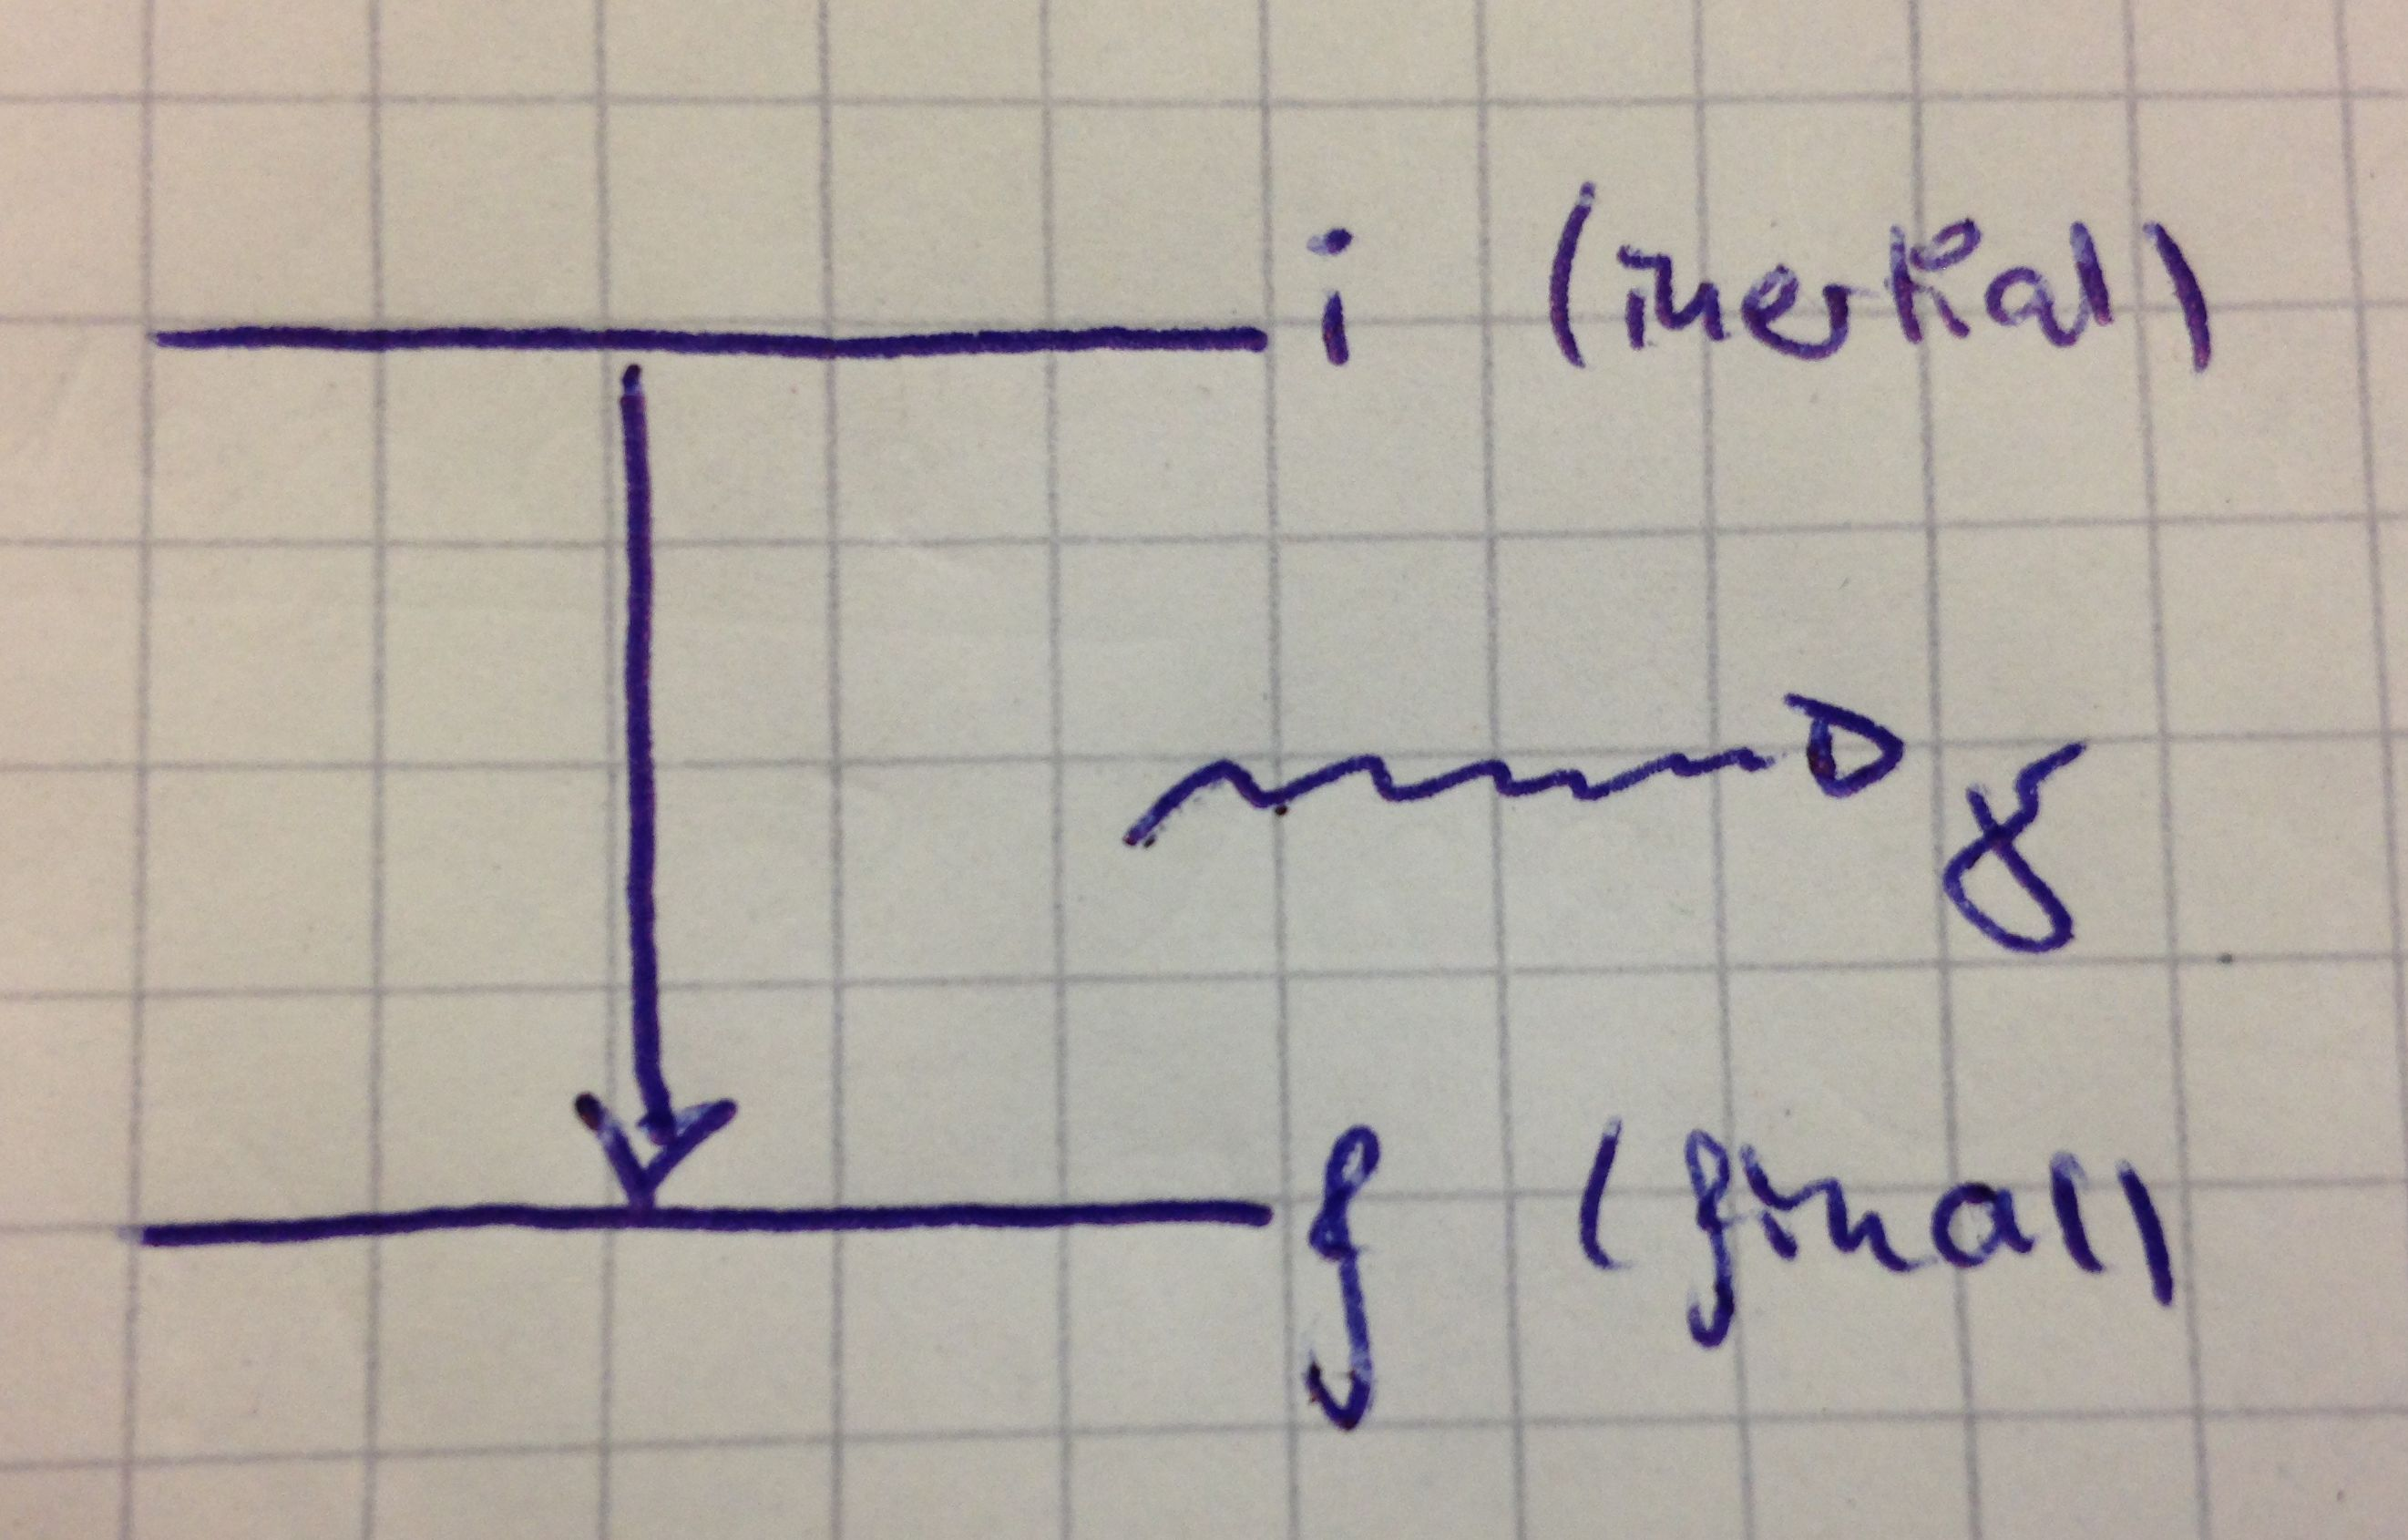
\includegraphics[width=8cm]{Bild2.jpg}
			\end{center}
		\end{figure*}
		\begin{align*}
		H &= H_e + H_\gamma & H_e &: \text{für Elektron}, ~ H_\gamma : \text{für Photon} \\
		H_e &= \underbrace{\frac{\vec{p}^2}{2 m_e} - e \Phi}_{\mathclap{H_e^0}}
		+ \frac{e \vec{A} \vec{p}}{m c}
		+ \frac{e^2}{2 m c^2} \vec{A}^2 &
		&\text{(Coulombeichung)}\\
		&= H_e^0 + H^1 + H^2 \\
		H_e^0 &= \frac{\vec{p}^2}{2 m} - Z \alpha \hbar c \frac{1}{r} & 
		Z &~\text{ist Kernladung},~ \alpha = \frac{e^2}{4 \pi \hbar c}\\
		H_e^0 \ket{n} &= E_n \ket{n} = \hbar \omega_n \ket{n} & 
		\ket{n} &~ \text{ist Elektronzustand}
		\end{align*}	
		für ein H-Atom:
		\begin{align*}
		E_n &= - \frac{1}{2} (Z \alpha)^2 m c^2 \frac{1}{n^2}
		= \frac{1}{2} Z \alpha \hbar c \overbrace{\erw{r^{-1}}}^{\mathclap{\frac{Z}{a_B n^2}}}
		= - \frac{1}{2 n^2} \frac{Z^2 \alpha \hbar c}{a_B} &
		a_B &= \frac{\hbar}{m \alpha c} \\
		H_\gamma &= \int \frac{\diff^3 k}{(2 \pi)^3}
		\sum_{\lambda \in \{+,-\}} \hbar \omega_k
		~a_\lambda (\vec{k})~a^\dagger_\lambda (\vec{k})
		\end{align*}
		Anfangszustand: 
		\begin{align*}
		\ket{i} &= \ket{n(\ell, \ell_z); 0} = \ket{n} \otimes \ket{0}
		\end{align*}
		wobei im \underline{ersten Term} $n$ die Hauptquantenzahl ist, die $\ell$'s sind eigentlich immer da, aber aus Faulheit schreiben wir die fast nie mit, die $0$ bedeutet, dass wir kein Photon haben. Im \underline{zweiten Term} ist $\ket{n}$ der Zustand vom H-Atom und $\ket{0}$ der Zustand von der elektromagnetischen Welle.
		
		Endzustand:
		\begin{align*}
		\ket{f} &= \ket{m(\ell', \ell_z'); \vec{k}, \lambda} 
		= \ket{m} \otimes \ket{\vec{k}, \lambda}
		\end{align*} 
		Der Energieunterschied ist dann:\footnote{Ich habe den Betrag in $\omega_{mn}$ gesetzt, damit wir nicht mit Minuszeichen oder so durcheinander kommen.}
		\begin{align*}
		\Delta E &= E_f - E_i = \hbar 
		\underbrace{(|\omega_m - \omega_n)|}_{\mathclap{\omega_{mn}}} 
		+ \hbar c |\vec{k}| = \hbar (\omega_{mn} + \omega_k)
		\end{align*}
		Übergangsrate: 
		\begin{align*}
		W_{f \leftarrow i} &= 
		\int \frac{\diff^3 k}{(2 \pi)^3} \sum_\lambda
		\frac{2 \pi}{\hbar^2} \delta(\omega_{mn} + \omega_k)
		\left|\braket{f | H_e^1 + H_e^2 | i}\right|^2
		\end{align*}	
		Und $H_e^1 + H_e^2$ ist die Störung (Lösung für $H_e^0 + H_\gamma$ ist bekannt).
		
		Mit Hilfe von
		\begin{align*}
		\int \diff^3 k &= \int \diff k ~k^2 \int \diff \Omega_k
		= \frac{1}{c^3} \int \diff \omega_k ~\omega^2 \int \diff \Omega_k
		\end{align*}
		Können wir schreiben:
		\begin{align*}
		W_{f \leftarrow i} &= \int \diff \Omega_k 
		\frac{\omega_{mn}^2}{4 \pi^2 \hbar^2 c^3}
		\sum_\lambda 
		\left|\braket{f | H_e^1 + H_e^2 | i}\right|^2 \\
		\braket{f | H_e^1 | i} &= 
		\frac{e}{mc} \braket{m | \braket{\vec{k} , \lambda | \hat{\vec{A}}(\vec{k}) | 0} \hat{p} | n} & &\vec{A}\text{~Operator nicht diagonal im Photonraum}
		\end{align*}
		\begin{align*}
		\braket{\vec{k} ,\lambda | \vec{A} (\vec{r}) | 0} &= 
		\sqrt{\hbar} \int \frac{\diff^3 k'}{(2 \pi)^3} \frac{c}{\sqrt{2 \omega_k}}
		\sum_{\lambda'} \vec{\epsilon}_{\lambda'} (\vec{k}') e^{-i \vec{k}' \vec{r}} 
		\cdot \braket{0 | a_\lambda (\vec{k}) a_{\lambda'} (\vec{k}') | 0} 
		\end{align*} 
		Hierbei ist gut zu wissen, dass $\ket{\vec{k} , \lambda} = a_\lambda^\dagger \ket{0}$ und $\bra{\vec{k}, \lambda} = \bra{0}a_\lambda (\vec{k})$.
		\begin{align*}
		\braket{0 | a_\lambda (\vec{k}) a_{\lambda'} (\vec{k}') | 0} &=
		\braket{0 | 
			\underbrace{\left[ a_\lambda (\vec{k}), a_{\lambda'} (\vec{k}') \right]}_{\mathclap{\delta_{\lambda \lambda'} (2 \pi)^3 \delta^{(3)}(\vec{k} - \vec{k'}) \mathds{1}}}  
			| 0} \\
		\braket{\vec{k}, \lambda | \vec{A} (\vec{r}) | 0} &=
		\sqrt{\frac{\hbar}{2 \omega_k}} c~ \vec{\epsilon}_\lambda (\vec{k}) e^{-i \vec{k} \vec{r}} \\
		\braket{f | H_e^1 | i} &= 
		\frac{e}{m} \sqrt{\frac{\hbar}{2 \omega_k}}
		\braket{m | e^{-i \vec{k} \vec{r}} \vec{\epsilon} \vec{p} | n} 
		\end{align*}
		Im Übrigen gilt $\omega_k = |\omega_n - \omega_m| = |-\omega_{mn}| = |\omega_{nm}|$ (siehe $\delta-$Fkt. oben)
		
		Dipolapproximation:
		\begin{align*}
		e^{-i \vec{k} \vec{r}} &= 1 + \mathscr{O} (Z\alpha) \\
		\vec{p} &= \frac{m}{\hbar} i \left[H_e^0, \vec{r}\right] \\
		\Rightarrow 
		\braket{f | H_e^1 | i} &= 
		\frac{-i e}{\sqrt{2}} \sqrt{\hbar \omega_k} 
		\braket{m | \vec{\epsilon}_\lambda \cdot \vec{r}| n}
		\end{align*}
		\begin{align*}
		W_{f \leftarrow i} &= \frac{\omega_{mn}^2 e^2}{8 \pi^2 \hbar c^3}
		\int \diff \Omega_k \sum_\lambda \left|\braket{m | \vec{\epsilon}_\lambda (\vec{k}) ~\vec{r} | n}\right|^2
		\end{align*}
		Der Beitrag im Betrag ins Quadrat ist
		\begin{align*}
		\vec{\epsilon}_{\lambda i}^{~*} (\vec{k}) ~\vec{\epsilon}_{\lambda j} (\vec{k}) 
		\braket{m | r_i | n} \braket{n | r_j | m}
		\end{align*}
		Und mit dem Integral:
		\begin{align*}
		\int \diff \Omega_k (\vec{\epsilon}_{\lambda i}(\vec{k}))^2 &= \frac{4 \pi}{3} \\
		\frac{1}{4 \pi} \int \diff \Omega_k \sum_\lambda 
		\vec{\epsilon}_{\lambda i} (\vec{k}) ~\vec{\epsilon}_{\lambda j} (\vec{k}) 
		&= \frac{2}{3} \delta_{ij}
		\end{align*}
		Somit haben wir nun die Übergangsrate für Spontane Emission in Dipolapproximation:
		\begin{empheq}[box=\boxed]{align*}
		W_{f \leftarrow i} = \frac{\omega^3_{nm} e^2}{3 \pi \hbar c^3}
		\left|\braket{m | \vec{r} | n}\right|^2 
		= \frac{4}{3} \frac{\omega_{nm}^3 \alpha}{c^2}
		\left|\braket{m | \vec{r} | n}\right|^2
		\end{empheq}
		Spontane Emission:
		\begin{equation*}
		W_{m \leftarrow n} = A_{mn} = \frac{4}{3} \frac{\omega_{nm}^3 \alpha}{c^2}
		\left|\braket{m | \vec{r} | n}\right|^2
		\end{equation*}
		Induzierte Emission:
		\begin{equation*}
		W_{m \leftarrow n} = B_{mn} u (\omega_{nm})
		= \frac{4 \pi e^2}{3 \hbar^2} \left|\braket{m | \vec{r} | n}\right|^2
		u (\omega_{nm})
		\end{equation*}
		Induzierte Absorption
		\begin{equation*}
		W_{n \leftarrow m} = B_{nm} u(\omega_{nm})
		\end{equation*}
		Und $B_{mn} = B_{nm}$ sind Einsteinkoeffizienten.
		
		$N_n$ Atome im Zustand $\ket{n}$
		
		$N_m$ Atome im Zustand $\ket{m}$
		
		Leistung:
		\begin{align*}
		\text{Spontane Emission} &:  
		&P_{SE} &= 
		\overbrace{N_n A_{mn}}^{\mathclap{\text{Rate~} \left[\frac{1}{\text{Zeit}}\right]}} 
		\underbrace{\hbar \omega_{nm}}_{\mathclap{\text{Energie}}}\\
		\text{Induzierte Emission} &:
		&P_{IE} &= N_n B_{mn} ~\hbar \omega_{nm} ~u(\omega_{nm})\\
		\text{Induzierte Absorption} &:
		&P_{IA} &= N_m B_{mn} ~\hbar \omega_{mn} ~u(\omega_{nm}) < 0
		\end{align*}
		2 Zustandssysteme $\ket{n}$, $\ket{m}$ im Wärmebad von Photonen im Gleichgewicht: 
		\begin{align*}
		N_n A_{mn} + (N_n B_{mn} - N_m B_{mn}) ~u(\omega_{nm}) &= 0 \\
		N_n &= \gamma \overbrace{e^{- \beta E_n}}^{\mathclap{Boltzmannfaktor}} 
		,& N_m &= \gamma e^{-\beta E_m}
		\end{align*}
		mit $\beta = \frac{1}{k_B ~T}$ \\
		$T$: Temperatur und $\gamma$: Konstante
		\begin{align*}
		\Rightarrow 
		e^{-\beta \hbar \omega_n} \left( A_{mn} + B_{mn} u(\omega_{nm}) \right)
		&= e^{-\beta \hbar \omega_{m}} B_{mn} u(\omega_{nm}) \\
		\Leftrightarrow u(\omega_{nm}) &= \frac{A_{mn}}{B_{mn}} \frac{1}{e^{\beta \hbar \omega_{mn}} - 1}
		\end{align*}
		Und das ist die Energiedichte des elektromagnetischen Feldes im thermischen Gleichgewicht $\left(T=\frac{1}{k_B \beta}\right)$.
		
		Planck:
		\begin{align*}
		\frac{A_{mn}}{B_{mn}} &= \frac{\hbar \omega_{nm}^3}{\pi^2 c^3} \\
		B_{mn} &= \frac{\pi e^2}{3 \hbar^2} \left|\braket{n | \vec{r} | m}\right|^2 \\
		A_{mn} &= \frac{\omega_{mn}^3 e^2}{3 \pi \hbar c^3} \left|\braket{n | \vec{r} | m}\right|^2 
		= \frac{4}{3} \frac{\omega_{mn}^3}{c^2} \alpha \left|\braket{n | \vec{r} | m}\right|^2 
		\end{align*}
		\subsection{Beispiel: $2p \rightarrow 1s$ Wasserstoff: Spontane Emission}
		\begin{figure*} [h]
			\begin{center}
				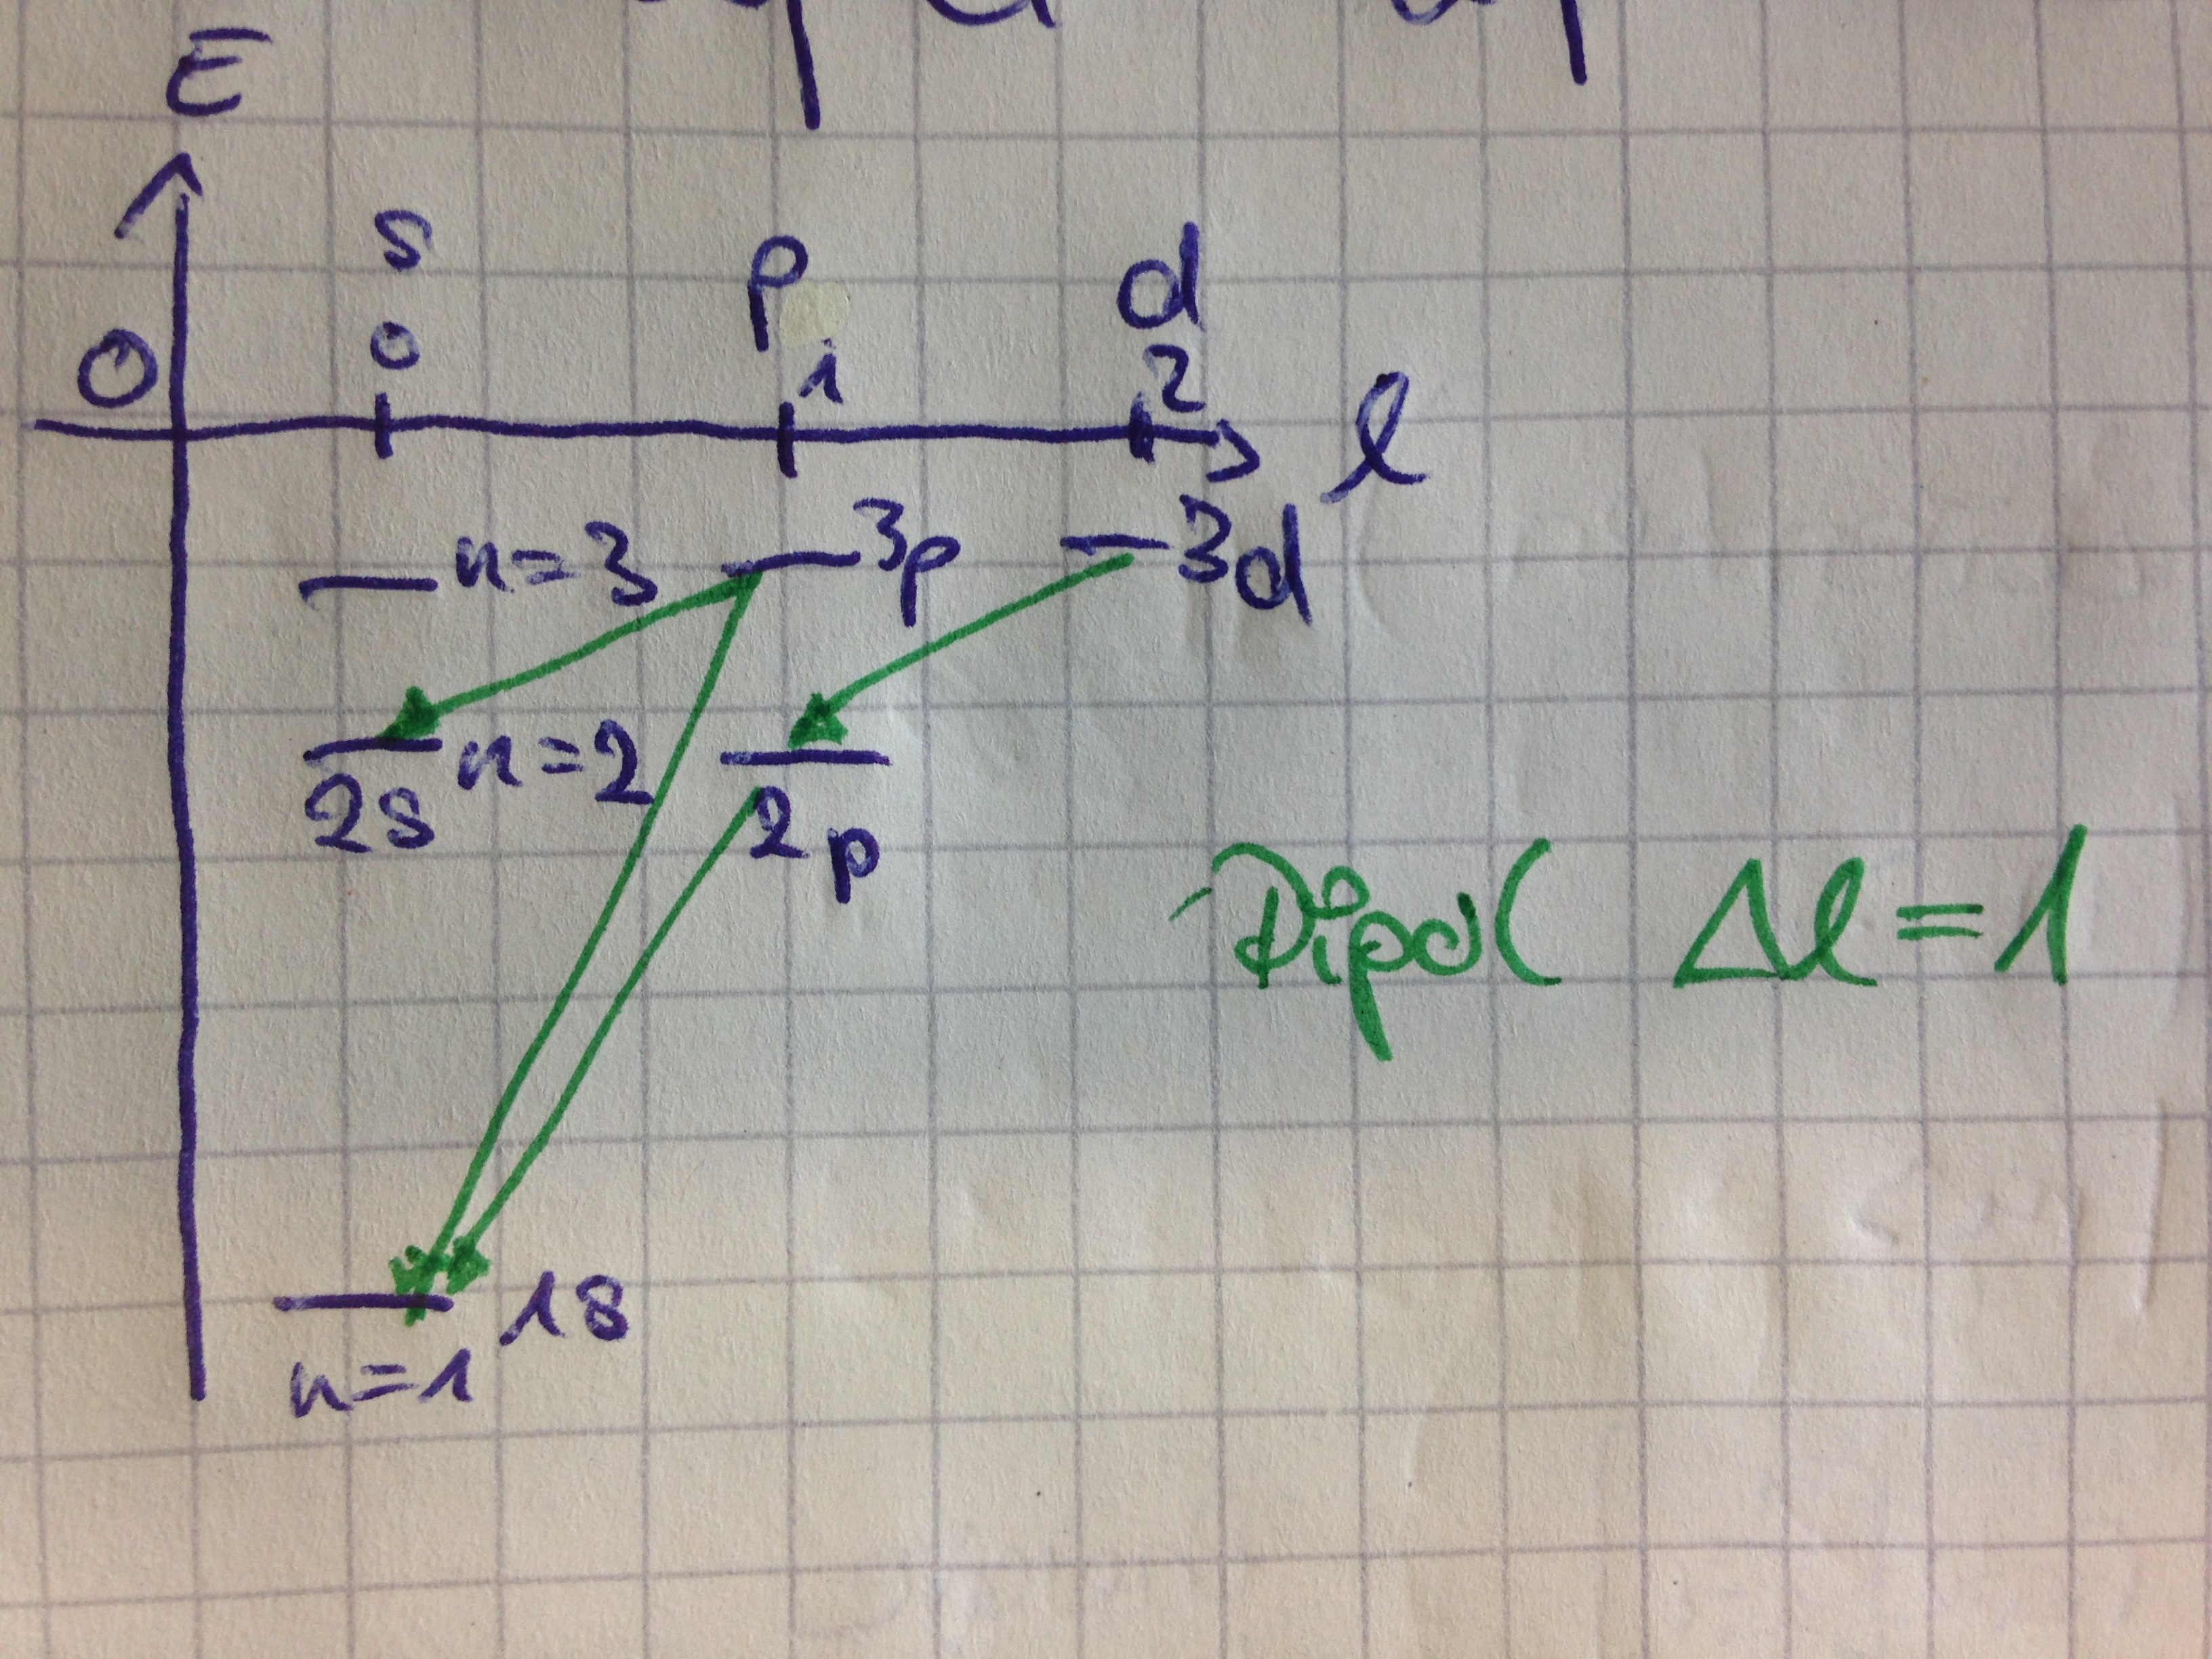
\includegraphics[width=10cm]{Bild3.jpg}
			\end{center}
		\end{figure*}
	Überrgangsrate:\marginpar{02.11.2015}
		\begin{align*}
			W_{f \leftarrow i} &=
			\frac{4}{3} \frac{\alpha ~\omega_{if}^3}{c^2} 
			\left|\braket{f | \vec{r} | i}\right|^2
			& &\left( \text{Einheit}: ~\frac{1}{\text{Zeit}}\right)
		\end{align*}
	Leistung
		\begin{align*}
			P &= \hbar \omega_{if} ~W_{f \leftarrow i} ~N_{H_{2p}} \propto \omega_{if}^4
		\end{align*}
	Hierbei ist $\hbar \omega_{if}$ die Energie und $N_{H_{2p}}$ die Anzahl der Wasserstoffatome im 2p Zustand.
		\begin{align*}
			\omega_{if} &= 
			\left( \frac{1}{n_f^2} - \frac{1}{n_i^2}\right)
			\frac{m c^2}{2 \hbar} \left(Z \alpha\right)^2
			= \frac{3}{8} \frac{m c^2}{\hbar} \left(Z \alpha\right)^2
		\end{align*}
	Hier: $n_f = 1, n_i = 2$ und die Summe in Klammern ist $>0$ da die Energie im Coulombpotential $<0$ ist.
		\begin{align*}
			\psi_{n \ell m} (\vec{r}) &= 
			\underbrace{\frac{u_{n \ell} (r)}{r}}_{\mathclap{R_{n \ell} (r)}}
			Y_{\ell m} (\Theta, \phi)
		\end{align*}
	Wir haben hier die Laguerre Polynome und somit:
		\begin{align*}
			u_{10} (r) &=
			2r \left(\frac{Z}{a_B}\right) e^{-\frac{Z r}{a_B}} \\
			u_{21} (r) &=
			\frac{2 r^2}{\sqrt{3}} \left(\frac{Z}{2 a_B}\right)^{\frac{3}{2}} e^{-\frac{Zr}{a_B}}
		\end{align*}
		\begin{align*}
			\frac{\vec{r}}{r} &=
			\sqrt{\frac{4\pi}{3}} 
			\left[
				\frac{1}{\sqrt{2}} \left(- Y_{11} + Y_{1-1}\right),
				\frac{1}{\sqrt{2}} i\left(Y_{11} + Y_{1-1}\right),
				Y_{10}
			\right]
		\end{align*}
	Winkelanteil von $\braket{i | \vec{r} | f}$ (Hier umgedreht, damit wir nicht komplex konjugieren müssen und wir den Braket sowieso ins Betragsquadrat nehmen.)
		\begin{align*}
			&\braket{\ell = 1, m | \vec{r} | 0~0} = & 
			&(\text{Auswahlregel~} \Delta \ell = 1) \\
			&= r \sqrt{\frac{4 \pi}{3}} \int \diff \Omega Y_{\ell m}^* (\Omega)
			\begin{pmatrix}
			\frac{1}{\sqrt{2}} \left(- Y_{11} + Y_{1-1}\right) \\
			\frac{1}{\sqrt{2}} i\left(Y_{11} + Y_{1-1}\right) \\
			Y_{10} \\
			\end{pmatrix}
			Y_{00}\\
			&= \frac{r}{\sqrt{6}} \delta_{\ell 1}
			\left( -\delta_{m1} + \delta_{m,-1}, i\delta_{m1} + i\delta_{m,-1}, \sqrt{2} \delta_{m0}
			\right)
		\end{align*}
	Radialintegral: 
		\begin{align*}
			\int_{0}^{\infty} \diff r ~r^2 \frac{u_{21} (r)}{r} ~r~ \frac{u_{10} (r)}{r} &=
			\int_{0}^{\infty} \diff r ~r~ u_{21} (r) ~ u_{10} (r) \\
			&= \frac{1}{\sqrt{6}} \left(\frac{Z}{a_B}\right)^4 
			\int_{0}^{\infty} \diff r ~r^4 e^{- \frac{3}{2} \frac{Zr}{a_B}} \\
			&= \left(\frac{2}{3}\right)^5 \frac{a_B}{Z} \frac{1}{\sqrt{6}}
			\underbrace{\frac{3}{2} \frac{Z}{a_B}
				\int_{0}^{\infty} \diff r \left(\frac{3}{2} \frac{Zr}{a_B}\right)^4
				e^{-\frac{3}{2} \frac{Zr}{a_B}}}_{\mathclap{4!}} \\
			&= \frac{a_B}{Z} \left(\frac{2}{3}\right)^5 \frac{24}{\sqrt{6}} 
			= \frac{a_B}{Z} \sqrt{6} ~\frac{2^7}{3^5}
		\end{align*}
	Jetzt benützen wir noch $(\delta_{m1})^2 = \delta_{m1}$ und $\delta_{m1}\delta_{m-1} = 0$ um den Erwartungswert auszurechnen:
		\begin{align*}
			|\braket{
				\overbrace{2~1~m }^{\mathclap{i}}| ~\vec{r}~ | \overbrace{1~0~0}^{\mathclap{f}}}|^2
				&= \frac{a_B^2}{Z^2} ~6~ \frac{2^{14}}{3^{10}} \frac{1}{6}
				\left(2 \delta_{m1} + 2 \delta_{m-1} + 2 \delta_{m0}\right) \\
				\Rightarrow W_{f \leftarrow i} &= 
				\frac{1}{3} \sum_{m=-1}^{1} \frac{4}{3} \frac{\alpha}{c^2}
				\left(\vphantom{\frac{3}{8}} \right.
					\underbrace{\frac{3}{8} \frac{m c^2}{\hbar} ~Z^2 \alpha^2}_{\mathclap{\omega_{if}}}
				\left. \vphantom{\frac{3}{8}} \right)^3 
				\frac{a_B^2}{Z^2} \frac{2^{15}}{3^{10}} 
				\left(\delta_{m1} + \delta_{m-1} + \delta_{m0}\right) \\
				&= \frac{2^8}{3^8} \frac{m c^2}{\hbar} Z^4 \alpha^5 
				\approx 6,3 \cdot 10^8 Z^4 s^{-1}
		\end{align*}
		
	\subsection{Quatrupolübergänge etc.}
	Matrixelement:
		\begin{align*}
			\braket{f | e^{-i \vec{k} \vec{r}} \vec{\epsilon} \cdot \vec{p} | i} \\
			e^{-i \vec{k} \vec{r}} &= 
			\sum_{j = 0}^{\infty} \frac{(-i)^j}{j!} 
			\underbrace{(\vec{k} \vec{r})^j}_{\mathclap{\mathscr{O} (Z \alpha)^j}} \\
			\text{wobei gilt:~} r &\approx Z a_B ,&
			|\vec{k}| &= \frac{\omega}{c} = \frac{\hbar \omega}{\hbar c} 
			\sim \frac{Z^2 \alpha \hbar c}{2 a_B \hbar c} 
			& &\rightarrow |\vec{k}| r \sim \frac{Z \alpha}{2} \\
			\text{kann nicht sein, einsetzen!}\\
			\text{Wir nehmen lieber:~} r &\approx \frac{a_B}{Z}
		\end{align*} 
		\begin{align*}
			\Rightarrow e^{-i \vec{k} \vec{r}} &=
			\underbrace{1}_{\mathclap{\text{Dipoloperator}}}
			- \overbrace{i \vec{k} \vec{r}}^{\mathclap{\mathscr{O} (Z \alpha)}}
			+ \underbrace{\ldots}_{\mathclap{\mathscr{O} (Z\alpha)^2}}
		\end{align*}
	Was ist mit $(\vec{k} \cdot \vec{r})(\vec{\epsilon} \cdot \vec{p})$?
		\begin{align*}
			(\vec{k} \cdot \vec{r})(\vec{\epsilon} \cdot \vec{p}) &=
			\frac{1}{2} \left[
				(\vec{k} \cdot \vec{r})(\vec{\epsilon} \cdot \vec{p})
				+ (\vec{\epsilon} \cdot \vec{r})(\vec{k} \cdot \vec{p})
				+ (\vec{k} \cdot \vec{r})(\vec{\epsilon} \cdot \vec{p})
				- (\vec{\epsilon} \cdot \vec{r})(\vec{k} \cdot \vec{p})
			\right] \\
			&= \underbrace{\frac{1}{2} \left[
				(\vec{k} \cdot \vec{r})(\vec{\epsilon} \cdot \vec{p})
				+ (\vec{\epsilon} \cdot \vec{r})(\vec{k} \cdot \vec{p})
			\right]}_{\mathclap{\text{elektrischer Quadrupol}}}
			+ \underbrace{\frac{1}{2} 
			(\vec{k} \times \vec{\epsilon})(\vec{r} \times \vec{p})}_{\mathclap{\text{magnetischer Dipol}}}
		\end{align*}
	Nützliche Relation: 
		\begin{equation*}
			\vec{p} = \frac{im}{\hbar} [H^0, \vec{r}]
		\end{equation*}
	Auswahlregeln:
	
	\begin{tabular}{l l} 
		$3d \rightarrow 1s$ & verboten als Dipolübergang, aber erlaubt als elektrischer  \\
		& Quadrupolübergang \\
		$3d \rightarrow 2p \rightarrow 1s$ & ist elektrischer Dipolübergang und hat höhere Rate
	\end{tabular}
	%Kap 2
	\section{Streutheorie}
	\section{Streutheorie}
	\subsection{Stationäres Streuproblem und Wirkungsquerschnitt}
	BILD
		
	Stromdichte des einlaufenden Teilchenstrahls: $\vec{j}_{ein}$
	\\
	BILD
	
	Anzahl der Teilchen, die durch $\diff \vec{A}$ läuft:
		\begin{align*}
			\diff N &= 
			\underbrace{\vec{j}_{ein} \cdot \diff \vec{A}}_{\mathclap{\text{Strom}}}
			\cdot \diff t
		\end{align*}
	NOCH EIN BILD
		\begin{align*}
			\diff A &= r^2 \diff \Omega = r^2 \diff \Theta \sin \Theta \diff \phi
		\end{align*}
	Differentieller Wirklungsquerschnitt $(r \rightarrow \infty)$
		\begin{empheq}[box=\boxed]{align*}
			\frac{\diff \sigma}{\diff \Omega} &=
			\frac{1}{|\vec{j}_{ein}|} \frac{\diff N}{\diff \Omega ~\diff t}
		\end{empheq}
	Homogener Strahl von Punktteilchen : $\vec{j} = \vec{v} \rho$ ($\rho$ ist Dichte)
		\begin{empheq}[box=\boxed]{align*}
			\frac{\diff \sigma}{\diff \Omega} &=
			\frac{|\vec{j}_{aus}(r, \Theta, \phi)|}{|\vec{j}_{ein}|} ~r^2
		\end{empheq}
	$ \leadsto |\vec{j}_{aus}| \propto \frac{1}{r^2}$ (bei gleichen Detektorflächen $\diff A$)
	
	Totaler Wirkungsquerschnitt:
		\begin{align*}
			\sigma = \int \diff \Omega \frac{\diff \sigma}{\diff \Omega}
		\end{align*}
	Beispiel: Streuung an Scheibe der Fläche A:
	\\
	BILD
	\\
		\begin{align*}
			\sigma &= \int \diff \Omega \frac{\diff \sigma}{\diff \Omega}
			= \frac{1}{|\vec{j}_{ein}|} \int \diff \Omega \frac{\diff N}{\diff \Omega ~\diff t}\\
			&= \frac{1}{|j_{ein}|} \frac{\diff N}{\diff t} & &\frac{\diff N}{\diff t}: 
			\text{~Zahl gestreuter Teichen pro Zeit} \\
			&= \frac{1}{|j_ein|} \cdot |j_{ein}| \cdot A = A
		\end{align*}
	Schrödingergleichung: 
		\begin{equation*}
			i \hbar \frac{\partial \Psi (\vec{r}, t)}{\partial t} = H \Psi (\vec{r} , t) 
		\end{equation*}
	Einlaufendes Wellenpaket
	
	BILD
	
		\begin{equation*}
			\psi (\vec{r} , t) = 
			\int \frac{\diff^3 k}{(2 \pi)^3} A(\vec{k}) e^{i(\vec{k} \vec{r} - \omega(\vec{k}) t)}
		\end{equation*}
	Annahme:
		\begin{align*}
			v_G << c &\Rightarrow \omega(\vec{k}) = \frac{\hbar \vec{k}^2}{2 m} & &(V(\vec{r}) = 0 (\text{Potential}))
		\end{align*}
	Nebenbemerkung:
	
	Wir kennen bislang nur die nichtrelativistische Quantenmechanik. Die Streutheorie relativistischer Teilchen unterscheidet sich nicht \underline{wesentlich}.
	
	Bild
	
		\begin{align*}
			r &>> R ,& r &>> \lambda = \frac{2 \pi}{k} &\Rightarrow 
			&\text{gestreute Welle ist \underline{lokal} eine Kugelwelle} 
		\end{align*}
	Betrachte \underline{elastische} Streuung an Kugelsymmetrischem Störpotenial $V(r)$:
		\begin{align*}
			\psi_S (\vec{r}, t) &= 
			\int \frac{\diff^3 k}{(2 \pi)^3} A(\vec{k}) \phi_S (\vec{r}, \vec{k})
			e^{-i \omega (\vec{k}) t} \\
			&\text{Einfallender Strahl:} & \phi_0 (\vec{r}) &= e^{i \vec{k}_0 \vec{r}} = e^{i k_0 z}\\
			&\text{Gestreuter Strahl:} & \phi_S (\vec{r}) 
		\end{align*}
	Für $r >> R$: Asymptotisch freie Wellen
	
	Einfallender Strahl:
		\begin{align*}
			\vec{p} &= \hbar k_0 \vec{e}_z ,& E &= \frac{\hbar^2 k_0}{2 m}\\
			-\frac{\hbar^2}{2 m} \vec{\nabla}^2 \phi_0 (\vec{r}) &= E \phi_0 (\vec{r})
		\end{align*}
	Wahrscheinlichkeitsstromdichte
		\begin{align*}
			\vec{j}_0 (\vec{r}, t) &=
			\frac{1}{2 m} 
			\left(\psi^* (\vec{r} , t) \vec{p} \psi (\vec{r}, t) - \psi (\vec{r}, t) \vec{p} \psi^* (\vec{r}, t)
			\right) \\
			&= \frac{\hbar k_0}{m} \vec{e}_z
		\end{align*}
	Nebenbemerkung: Teilchenstrom für $N_0$ Teilchen: $N_0 \frac{\hbar k}{m} \vec{e}_z$
	
	zu lösen ist:
		\begin{empheq}[box=\boxed]{align*}
			H \phi(\vec{r}) &= E \phi (\vec{r}) & &\text{für } E= \frac{\hbar k_0^2}{2 m} > 0\\
			H &= \frac{\vec{p}^2}{2 m} + V (r) & &V(r) \text{ begrenzt auf } r<R \\
			\phi (\vec{r}) &= e^{i k z} + \phi_S (\vec{r})
		\end{empheq}
	Ansatz:
		\begin{align*}
			\phi_S (\vec{r}) &\underset{r \rightarrow \infty}{\sim} f(\Theta) \frac{e^{i k_0 r}}{r} &
			&\text{mit Streuamplitude } f(\Theta)\\
			\vec{j} &= \frac{\hbar k_0}{m} \frac{|f(\Theta)|^2}{r^2}
			\hat{e}_r (\Theta , \phi) + \mathscr{O} \left(\frac{1}{r^3}\right)
		\end{align*}
		\begin{empheq}[box = \boxed]{align*}
			\frac{\diff \sigma}{\diff \Omega} = r^2 \frac{|\vec{j}_S|}{|\vec{j}_0|}
			= |f(\Theta)|^2
		\end{empheq}
	Dieser Ansatz löst die Schrödingergleichung für $r \rightarrow \infty$ 
		\begin{align*}
			\underset{r \rightarrow \infty}{\lim} r V(r) &= 0 &
			&(\text{kein Coulomb-Potential})
		\end{align*}
	Streutheorie \marginpar{5.11.15}
	
	Kurze Wiederholung \marginpar{heute nicht Bali}
	
	BILD
	
		\begin{align*}
			\diff A &= r^2 \diff \Omega ,& 
			\vec{j} &= \frac{\hbar}{2 m i} \left(\psi^* \vec{\nabla} \psi - \psi \vec{\nabla} \psi^* \right)
		\end{align*}
	$\diff N$ in diesem $\diff A$, in einem kleinen Zeitraum $\diff t$ \marginpar{??}
		\begin{align*}
			\frac{\diff \sigma}{\diff \Omega}
			&= \frac{|\vec{j}_{Streu}| ~\diff t ~ \diff A}{ |\vec{j}_{ein}| ~\diff t ~ \diff \Omega}
			=\frac{|\vec{j}_{Streu}| r^2}{|\vec{j}_{ein}|} :&
			&\text{hat Dimension Fläche}
		\end{align*}
	Annahmen:
		\begin{itemize}
			\item[-] 	Elastische Streuung, $\hbar k = \hbar k'$
			\item[-]	Stationäre Situation
			\item[-]	$V(\vec{r}) = V(|\vec{r}|)$ (Kugelsymmetrie)
			\item[-]	keine Absorption oder Emission
		\end{itemize}
	Wir wissen
		\begin{align*}
			\phi = \phi_0 + \phi_S = e^{i k z} + \phi_S
		\end{align*}
	$\phi$ ist im Bereich $r>R$ übereinstimmend mit Lösung der freien Schrödinger Gleichung.
		\begin{align*}
			\phi = \sum_{\ell = 0}^{\infty} R_\ell (r) 
			\underbrace{P_\ell (\cos \Theta)}_{\mathclap{\sqrt{\frac{4 \pi}{2\ell+1}} 
					Y_{\ell 0}(\cos \Theta)}} 
			& &[H, L_z] = 0 ~(\text{Drehimpulserhaltung})
		\end{align*}
	BILD \\
	\underline{Legendre-Polynome $P_\ell (\cos \Theta)$}
		\begin{align*}
			P_0 (\cos \Theta) &= P_0 (z) = 1\\
			P_1 (z) &= z
		\end{align*} 
	\subsection{Anwendung : Streuung an harter Kugel} \marginpar{09.11.2015}
	Harte Kugel:
	\begin{align*}
	V (r) =
	\left\{
	\begin{aligned}
	\infty , r &< R, \\
	0 , r &> r
	\end{aligned}
	\right.
	\end{align*}
	$\curvearrowright$ 
	$V(r)= 0$ für $r>R \rightarrow$ Schrödingergleichung $-\frac{\hbar^2}{2m} \vec{\nabla}^2 \phi(\vec{r})
	\propto \phi(\vec{r})$
	Einsetzen in Schrödingergleichung $\Rightarrow$ Bedingungen für Koeffizienten $R_\ell(r)$:
%		\begin{align*}
%			R_\ell(r) &= a_\ell j_\ell (kr) + b_\ell n_\ell (kr) ,& &\text{wobei}\\
%			j_\ell(\rho) &= (-\rho)^\ell \left(\frac{1}{\rho} \frac{\partial}{\partial \rho}\right)^\ell
%			\frac{\sin \rho}{\rho} :& &\text{sphärische Besselfunktion}\\
%			n_\ell(\rho) &= (-\rho)^\ell \left(\frac{1}{\rho} \frac{\partial}{\partial \rho}\right)^\ell
%			\frac{\cos \rho}{\rho} :& &\text{\sphärische Neumannfunktionen}
%		\end{align*}
	$\rho \rightarrow \infty : j_\ell (\rho) \simeq \frac{1}{\rho} \sin(\rho-\ell\frac{\pi}{2})$,
	$n_\ell (\rho) \approx -\frac{1}{\rho}  \cos(\rho-\ell\frac{\pi}{2})$
	
	Einfallende Welle (2.2) besteht an $j_\ell (kr)$
	
	Auslaufende Welle $ %geschwungen
	\frac{1}{r} e^{ikr}$ (Kugelwelle)
		\begin{align*}
			h_\ell^+ (\rho) &= j_\ell (rho) + in_\ell(\rho) %geschwungen mit unterschrift r \rightarrow \infty
			\frac{1}{i\rho} e^{i(\rho-\ell\frac{\pi}{2})} &
			&\text{(sphärische Hantelfunktion 1ter Art)} \\
			\Rightarrow \phi (\vec{r}) &= \sum_{\ell=0}^{\infty} (2 \ell +1) i^\ell
			\left[ j_\ell (kr) +\gamma_\ell h^+_\ell (kr)
			\right] P_\ell (\cos \Theta)
		\end{align*}
	Randbedingung: $\phi (R, \Theta, \phi)$
		\begin{align*}
			&\Rightarrow j_\ell (kR) + \gamma_\ell h_\ell^+(kR) = 0\\
			&\Rightarrow \gamma_\ell = -\frac{j_\ell(kR)}{h_\ell^+ (kR)}
		\end{align*}
	Streuamplitude:
		\begin{empheq}[box=\boxed]{align*}
			f(\Theta) = \sum_{\ell = 0}^{\infty} (2 \ell +1) \frac{\gamma_\ell}{ik} P_\ell(\cos \Theta)
		\end{empheq}
	Allgemein:
		\begin{align*}
			f(\Theta) &= \frac{1}{k} \sum_{\ell = 0}^{\infty}
			(2 \ell + 1) \underbrace{e^{i\delta_\ell} \sin \delta_\ell}_{\mathclap{-i \gamma_\ell}}
			P_\ell (\cos \Theta) \\
			\gamma_\ell &= \frac{1}{2} (e^{2i\delta_\ell} - 1)
			= -\frac{j_\ell(kR)}{j_\ell(kR)+ in_\ell (kR)}
		\end{align*}
		$\Rightarrow$
		\begin{empheq}[box=\boxed]{align*}
			\tan \delta_\ell = \frac{j_\ell (kR)}{n_\ell (kR)}
		\end{empheq}
		\begin{align*}
			\sigma &= \frac{4 \pi}{k^2} \sum_{\ell} (2\ell +1) 
			\frac{j_\ell^2 (kR)}{j_\ell^2 (kR)+ n_\ell^2 (kR)}
		\end{align*}
	Wobei der Bruch gleich $|\gamma_\ell|^2$
	
	Grenzfall 1: $kR \ll 1 (\gamma \gg R)$
		\begin{align*}
			j_\ell (\rho) &\underset{\rho \rightarrow 0}{\rightarrow} \frac{\rho^\ell}{(2\ell+1)!!}
			& n!! &= n(n-2) \ldots 
			& n_\ell (\rho) &\underset{\rho \rightarrow 0}{\rightarrow}
			-(2\ell + 1) !! \rho^{-(\ell +1)} \\
			\tan \delta_\ell &= -\frac{j_\ell (kR)}{n_\ell (kR)} &
			&\rightarrow - \frac{(kR)^{2\ell+1}}{(2\ell +1)!! (2\ell+1)!!} 
			& &= -\frac{(kR)^{2 \ell +1}}{(2\ell +1) [(2 \ell -1)!!]^2}
		\end{align*}
	kleine $\ell$ dominieren
		\begin{align*}
			\tan \delta_0 = - kR \approx \sin \delta \rightarrow 
			\sigma \approx \frac{\pi}{k^2} \sin^2\delta_0 + \text{höhere } \ell 
			\approx 4 \pi R^2 = 4 \sigma_{geom.}
 		\end{align*}
	Wellenlänge größer als ``Hindernis'' $\Rightarrow$ keine geom. Optik 
	\begin{figure*} [h]
		\begin{center}
			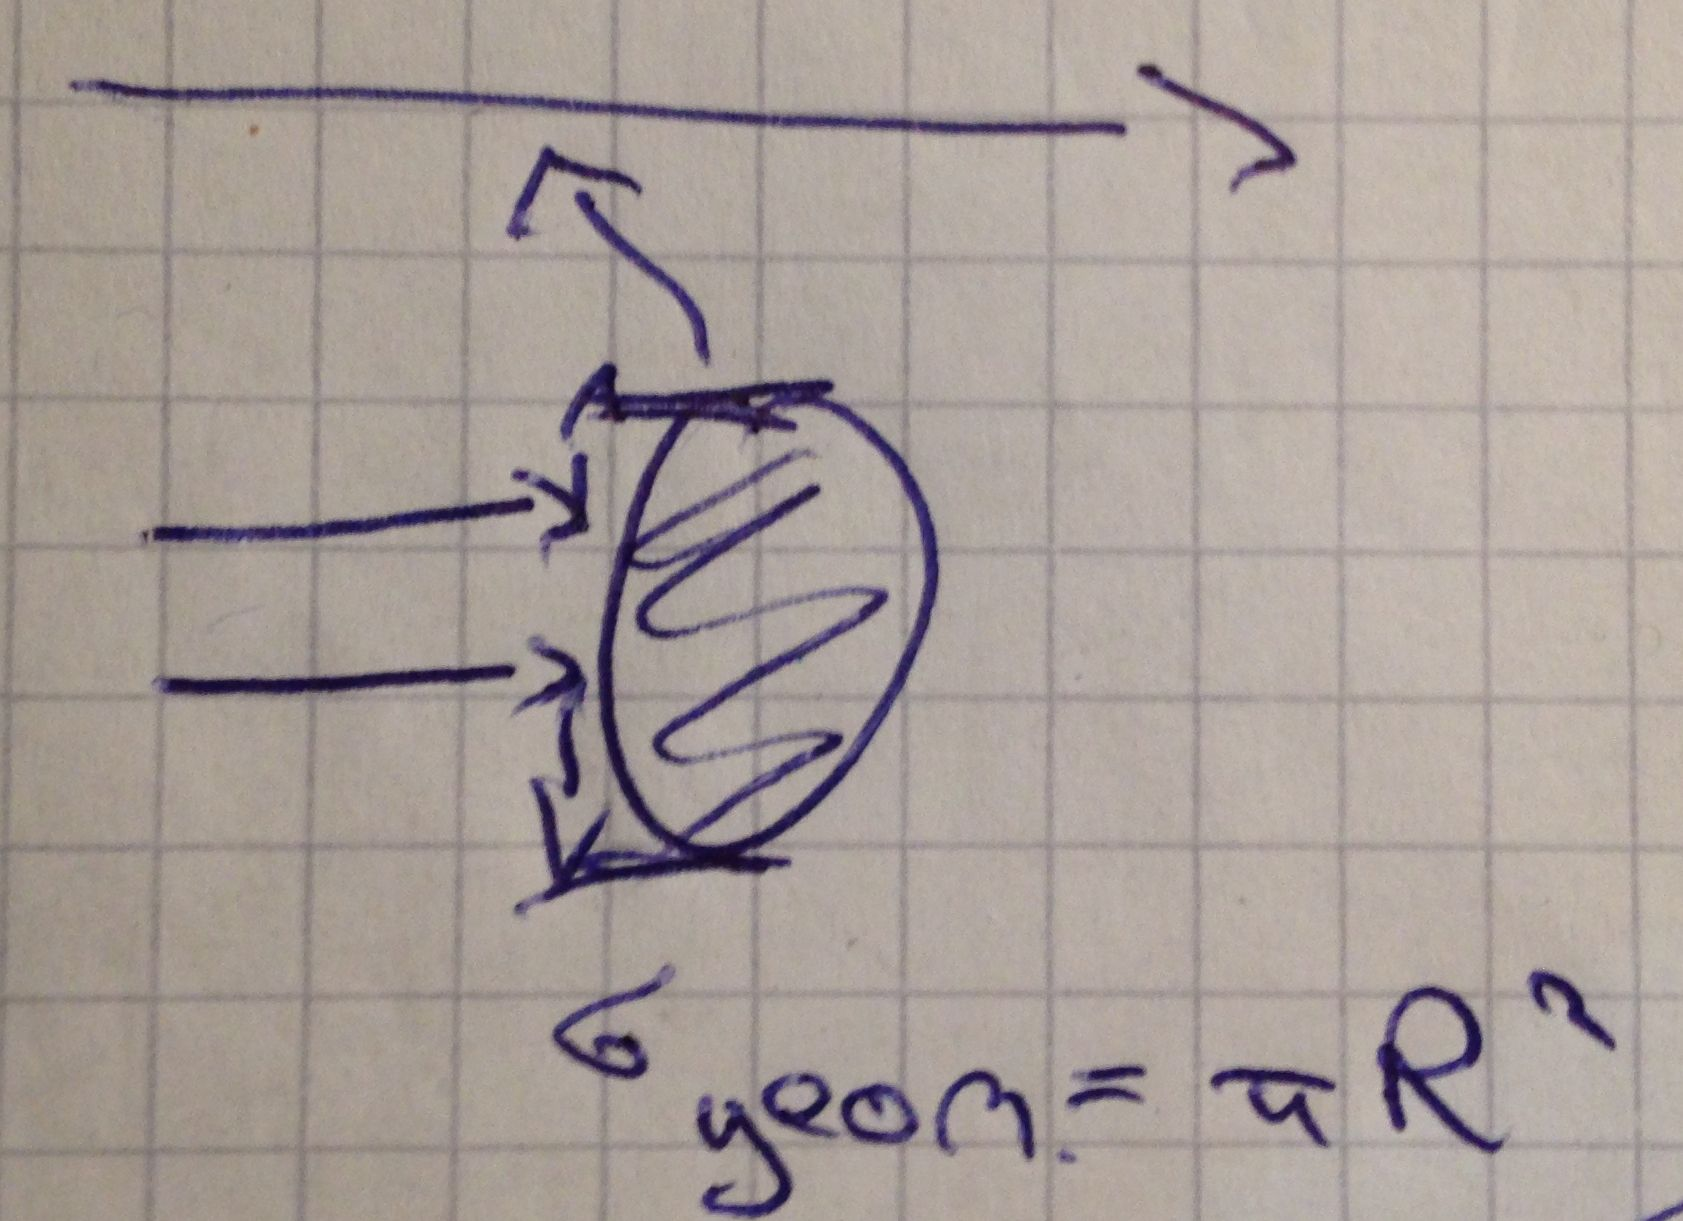
\includegraphics[width=8cm]{Annaherung_harte_Kugel1}
		\end{center}
	\end{figure*}
\FloatBarrier	
	2 Grenzfall $kR \gg1$
		\begin{align*}
			\tan \delta_\ell &\rightarrow - \frac{\sin (\rho-\ell \frac{\pi}{2})}{\cos (\rho-\ell \frac{\pi}{2})} 
			= -\tan (\rho-\ell \frac{\pi}{2}) = \tan(\ell \frac{\pi}{2} - \rho) \\
			\delta_\ell &\rightarrow \ell \frac{\pi}{2}- kR\\
			\sigma &\approx \frac{4 \pi}{k^2} \sum_{\ell =0}^{\approx int(kR)}
			(2 \ell + 1) \sin^2(\delta_\ell) 
			= \frac{4\pi}{k^2} \sum_\ell (2 \ell + 1) \sin^2(kR- \ell \frac{\pi}{2}) \\
			&\approx 2 \pi R^2 (1+ \mathscr{O} \left(\frac{1}{(kR)^{\frac{2}{3}}}\right)) 			
			\approx 2 \sigma_{geom.}
		\end{align*}
	Warum 2 $\sigma_{geom.}$? Für $\lambda \ll R$ ($k \gg \frac{1}{\ell}$) sollte klassischer Grenzfall gelten.
	\begin{figure*} [h]
		\begin{center}
			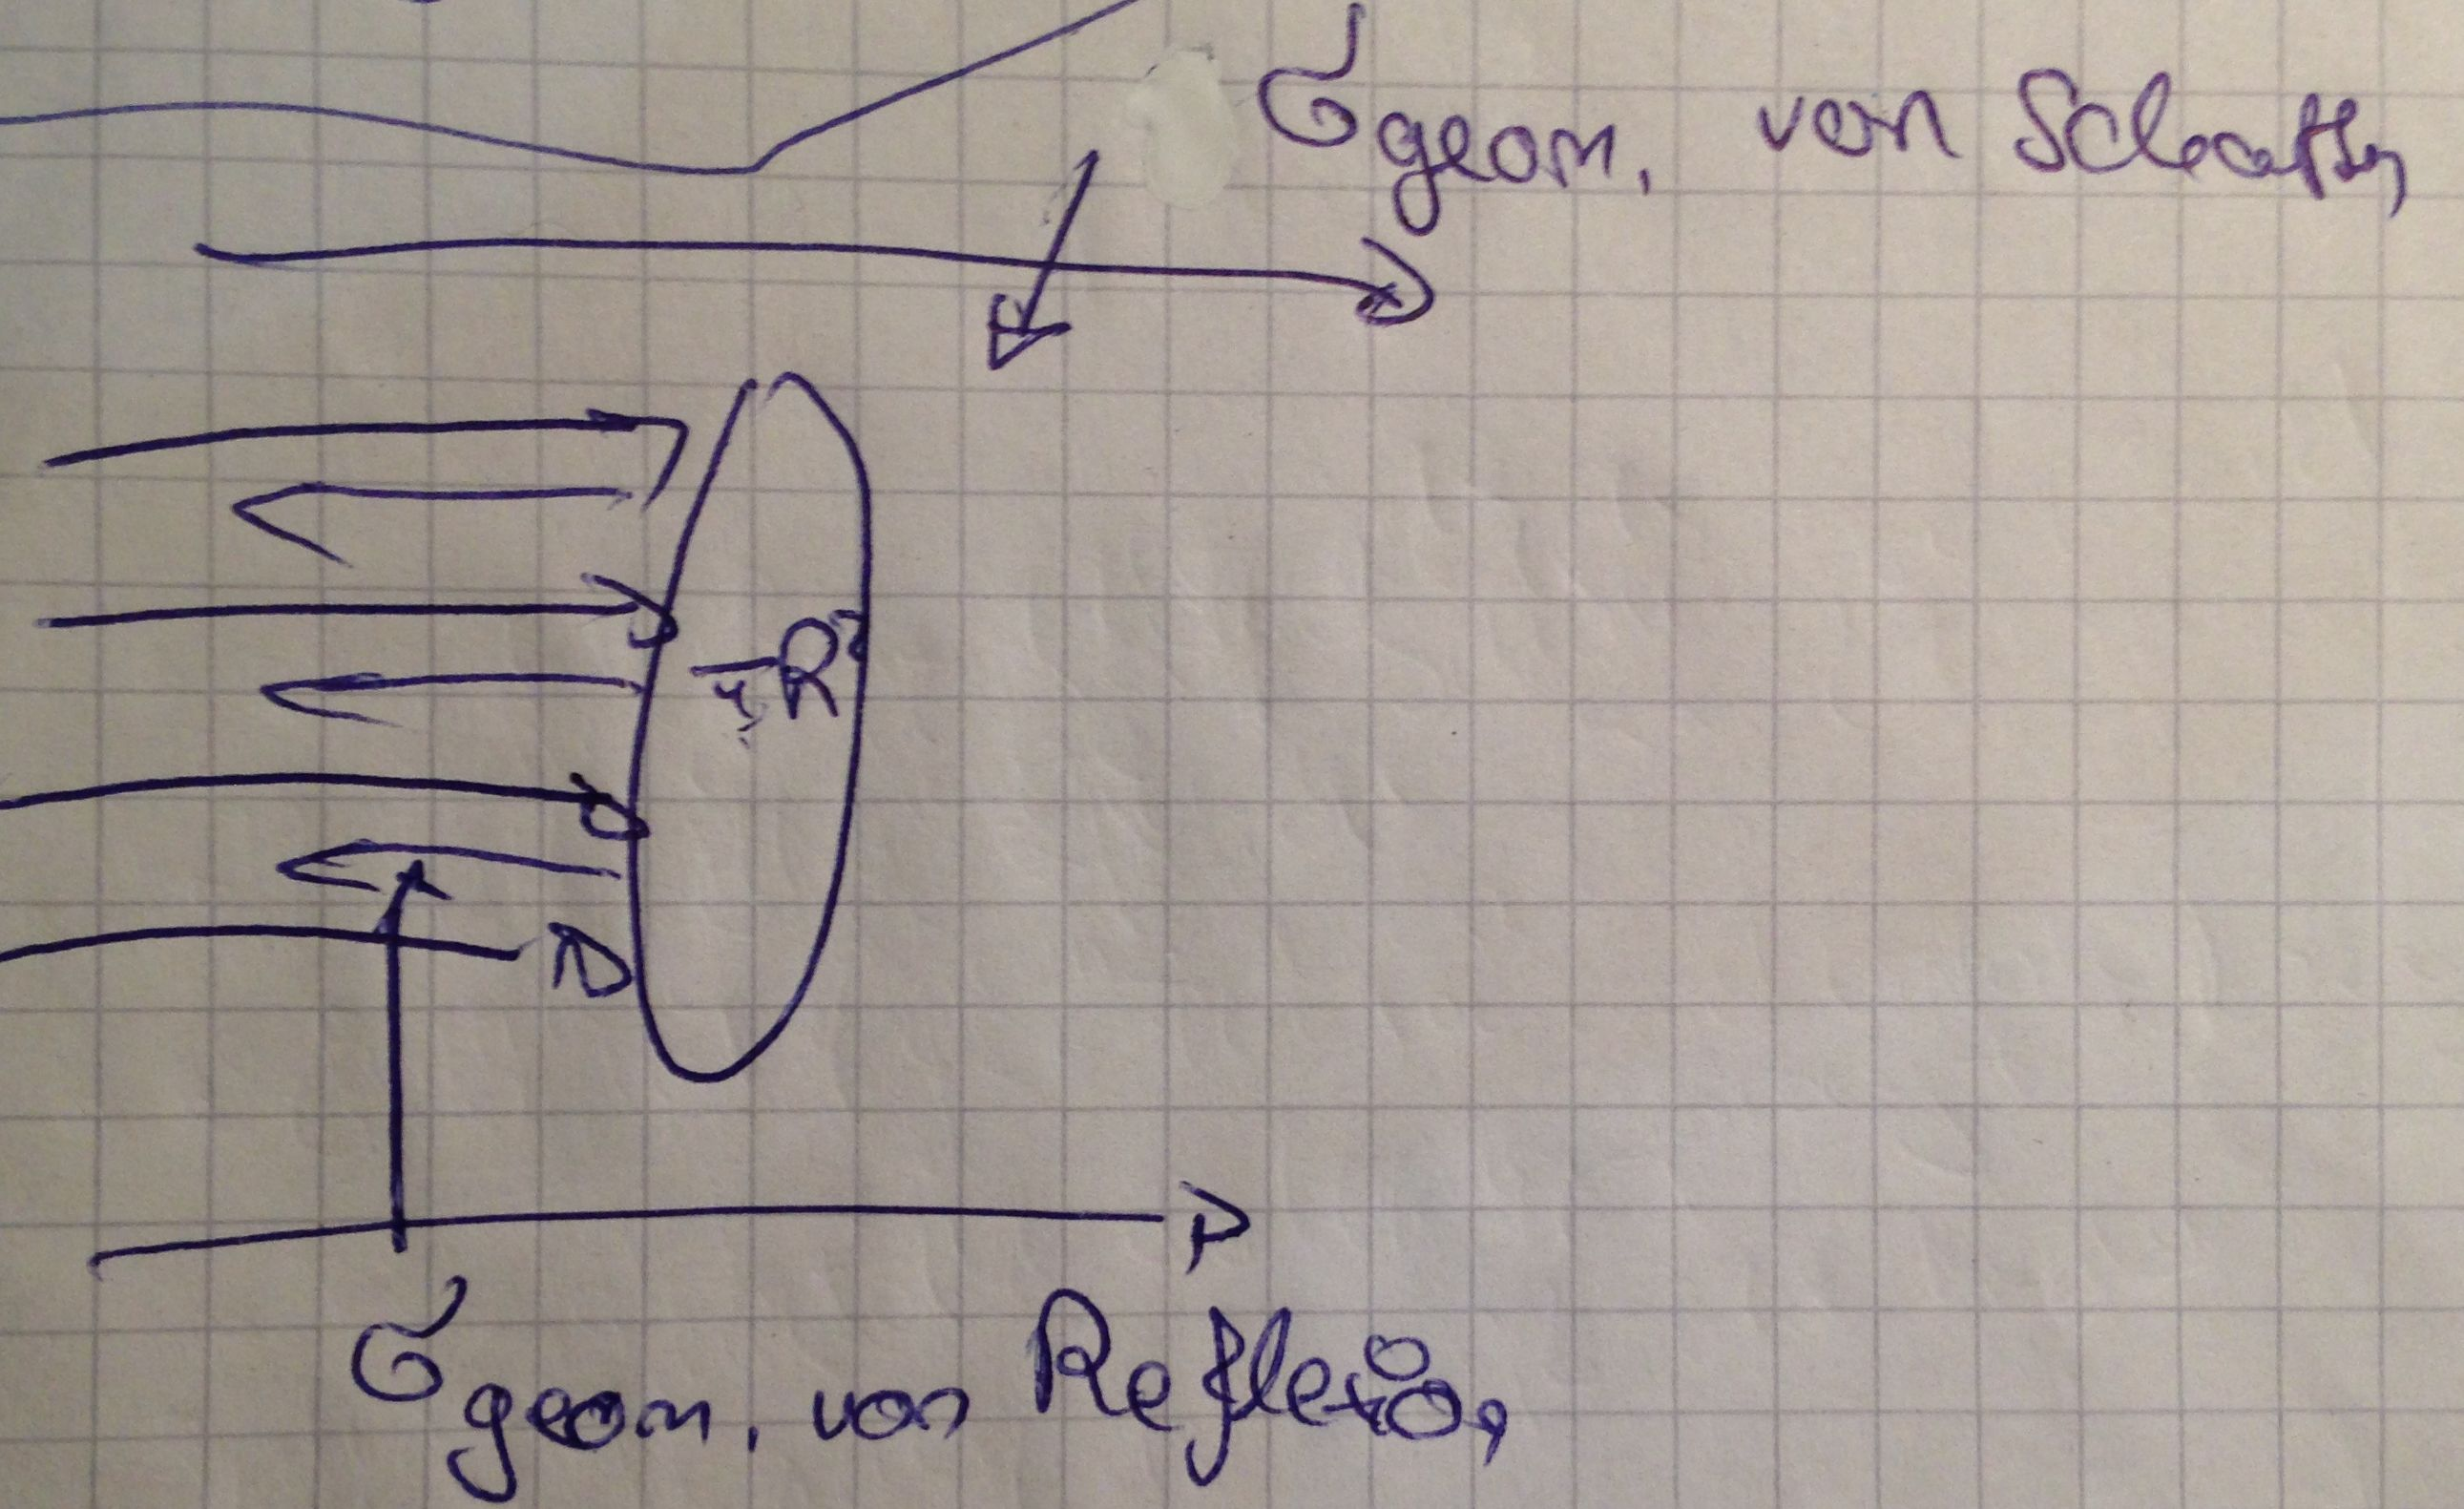
\includegraphics[width=8cm]{Annaherung_harte_Kugel2}
		\end{center}
	\end{figure*}	
	
	$\sigma$ ist so definiert, dass geometrische \textcolor{red}{Eingrpsdfjile} \marginpar{keine Ahnung was da stand}
	
	$\sigma = 2 \sigma_{geom.}$ ist
	\subsection{Die Born-Näherung}
	Schrödingergleichung:
		\begin{align*}
			\left(- \frac{\hbar^2}{2 m} \vec{\nabla}^2 + V (\vec{r})\right) \phi
			&= \frac{\hbar^2 k^2}{2m} \phi \\
			\left(\vec{\nabla}^2 - k^2\right) \phi(\vec{r}) 
			&= \frac{2m}{\hbar^2} V (\vec{r}) \phi (\vec{r})
		\end{align*}
	Homogene Gleichung:
		\begin{align*}
			\left(\vec{\nabla}^2 + k^2 \right) \phi_0 (\vec{r}) = 0 &
			&(\text{Helmholzgleichung}) 
		\end{align*}
	Greenfunktion
		\begin{align*}
			\left(\vec{\nabla}^2 + k^2 \right) G (\vec{r} - \vec{r}\,') 
			&= \delta^{(3)}(\vec{r} - \vec{r}\,') \\
			G(\vec{r}) &= 
			\int \frac{\diff^3 q}{(2 \pi)^3} e^{i \vec{q} \cdot \vec{r}} \tilde{G}(\vec{q})
			&\text{mit } \tilde{G} (\vec{q}) &= \frac{1}{k^2-q^2} \\
			&= \int \frac{\diff^3 q}{(2 \pi)^3} \frac{e^{i \vec{q} \cdot \vec{r}}}{k^2 - q^2} \\
			&\underset{\text{E-Dynamik}}{=} - \frac{e^{\pm i k r}}{4 \pi r}
		\end{align*}
	$+$ steht für retadierte Lösung (Ursache vor Streuung)
	
	\begin{figure*} [h]
		\begin{center}
			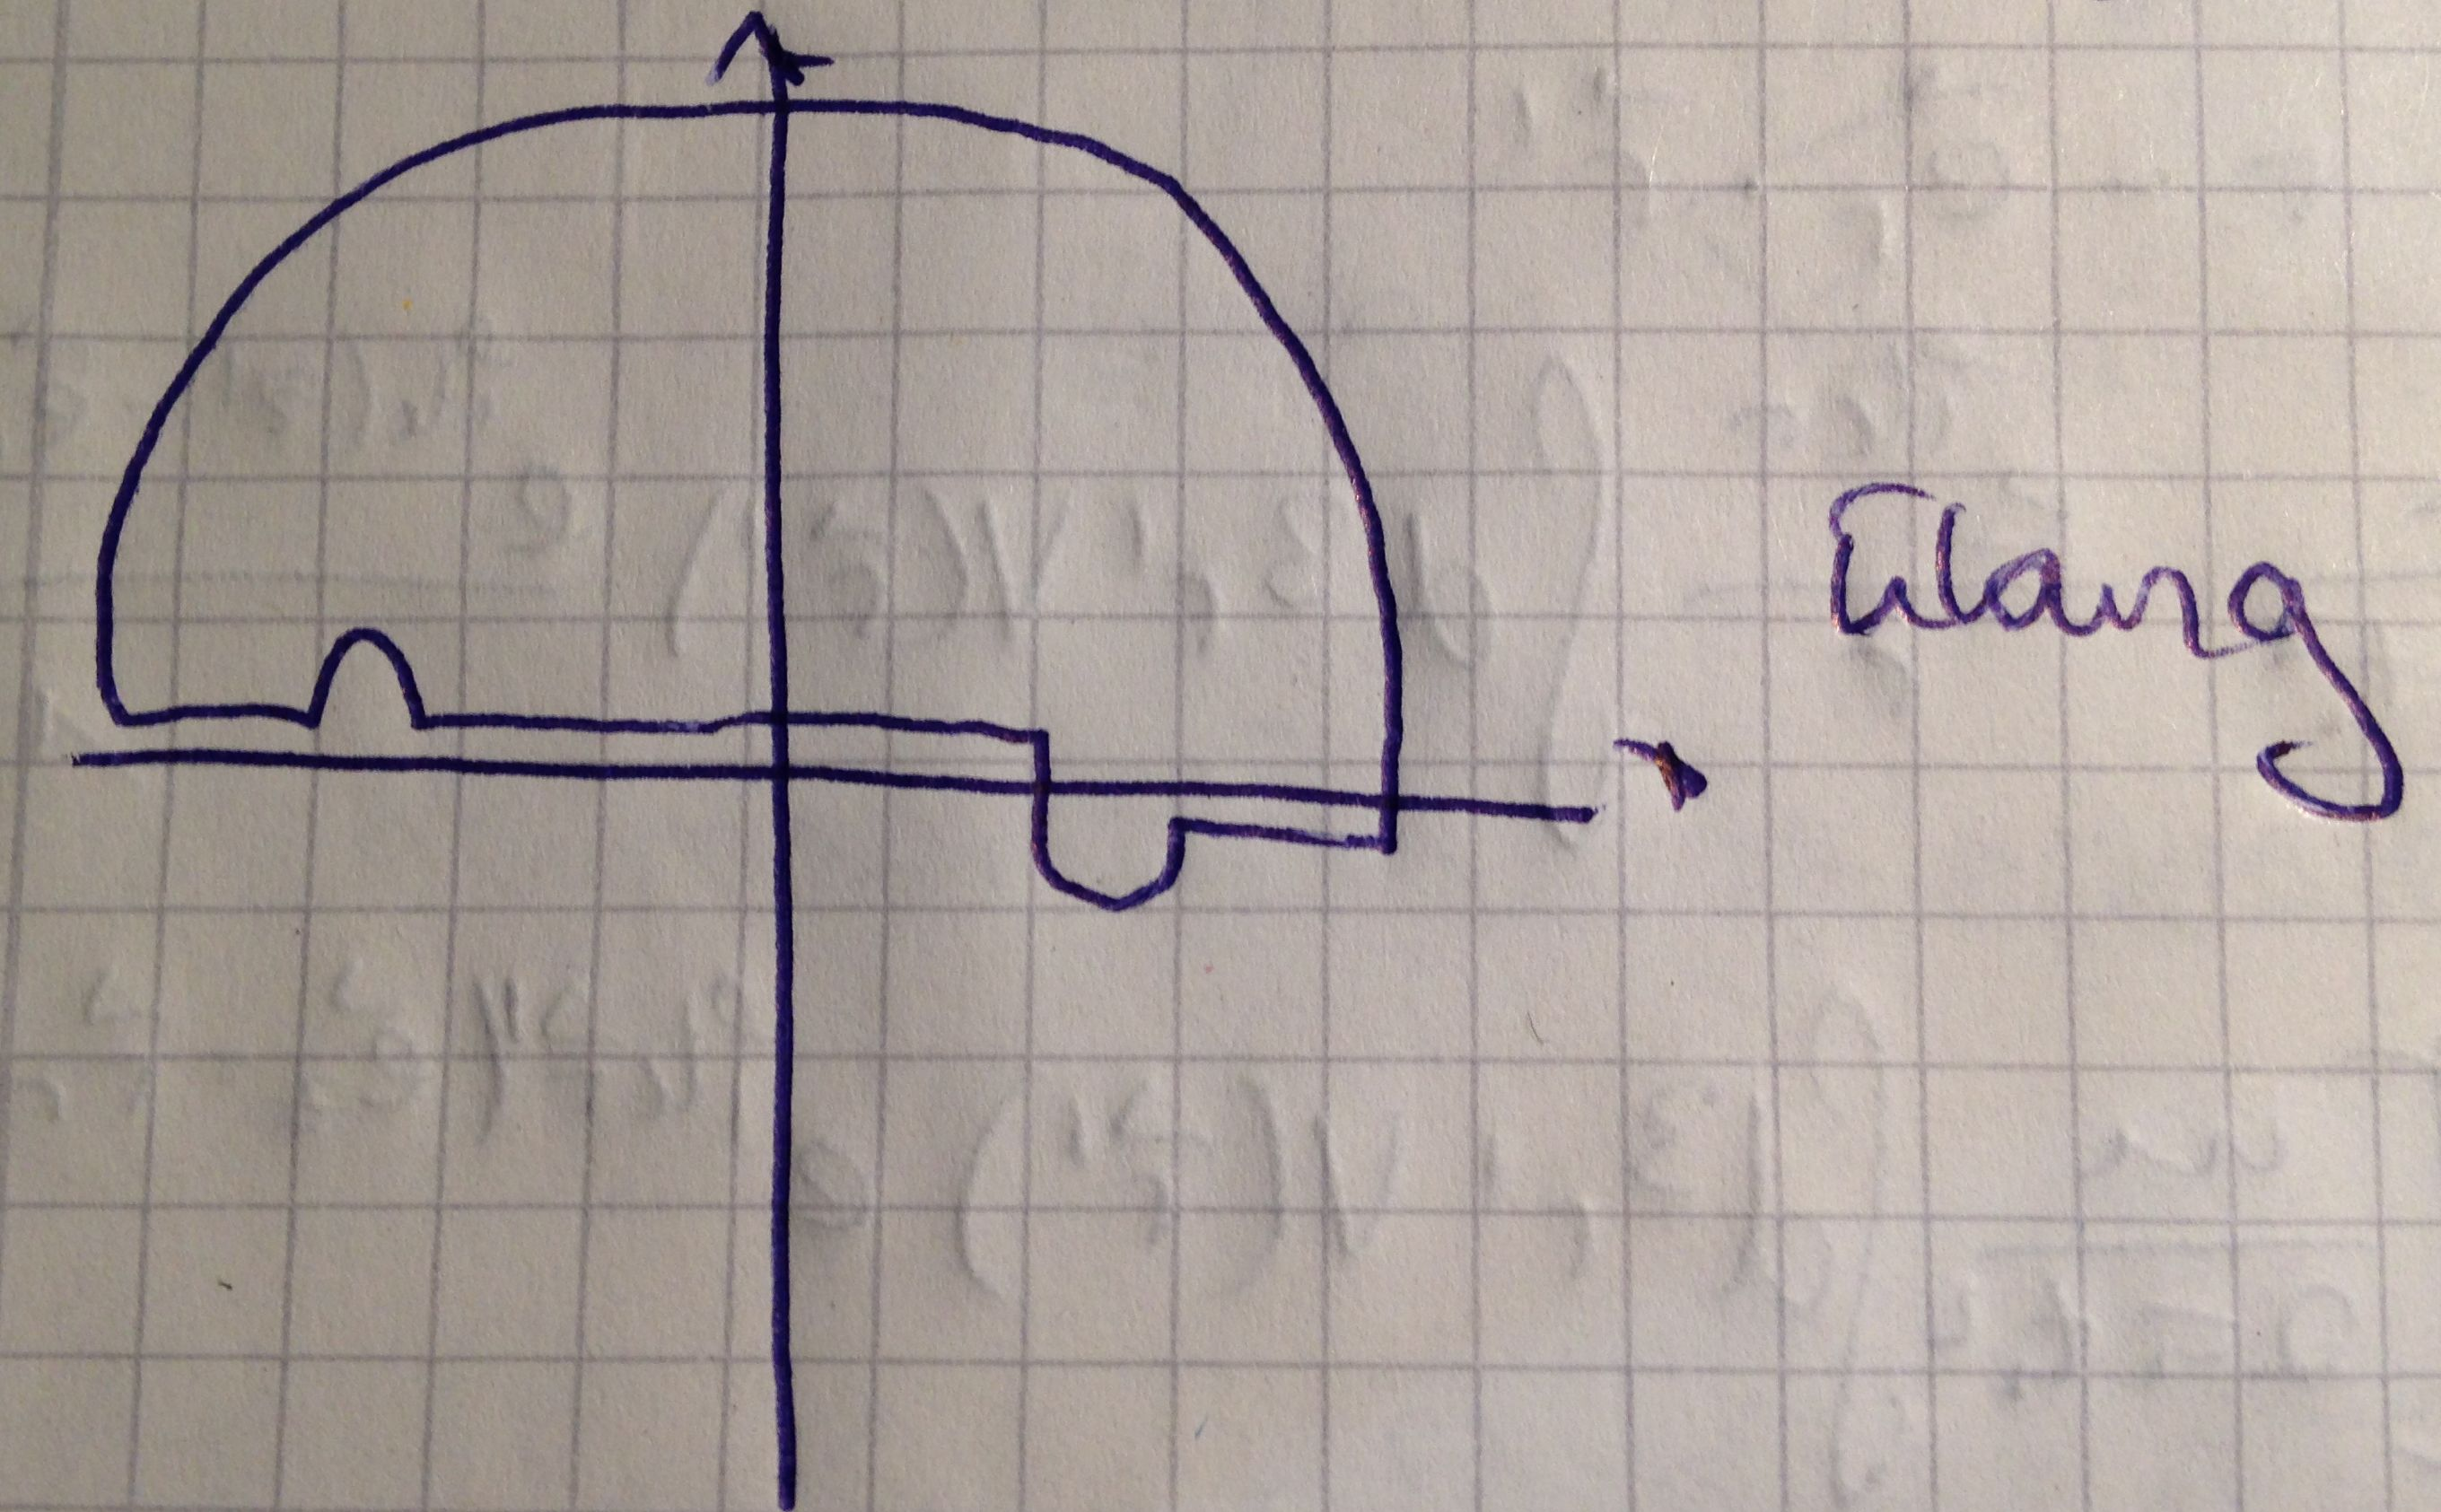
\includegraphics[width=8cm]{Born_Naeherung}
		\end{center}
	\end{figure*}
	Lösung der inhomogenen Gleichung:
		\begin{align*}
			\phi(\vec{r}) &= \phi_0 (\vec{r}) + 
			\int \diff^3 r' ~G(\vec{r} - \vec{r}\,') \frac{2m}{\hbar^2} V(\vec{r}\,') \phi (\vec{r}\,') \\
			&= \underbrace{e^{ikr \cos \theta}}_{\substack{\text{einlaufende Welle}}}
			\underbrace{- \frac{m}{2 \pi \hbar^2} \int \diff^3 r' ~V(\vec{r}\,') 
			\frac{e^{ik |\vec{r} - \vec{r}\,'|}}{|\vec{r} - \vec{r}\,'|} \phi (\vec{r}\,')}_{\mathclap{[
				B\phi] (\vec{r}) \text{ mit } ``B=\frac{2m}{\hbar^2} GV''}} 
		\end{align*}
		\begin{align*}
			\phi &= \phi_0 + B \phi &
			&\Rightarrow \phi_0 = \phi - B \phi = (1 - B) \phi \\
			\phi &= (\mathds{1} - B)^{-1} \phi_0 = \sum_{n = 0}^{\infty} B^n \phi_0 &
			&= \phi_0 + B \phi_0 + B^2 \phi_0 + \ldots \\
			& & &\text{\underline{Born-Reihe}}
		\end{align*}
	oder
		\begin{align*}
			\phi (\vec{r}) &= e^{ikr \cos \theta}
			- \frac{m}{2 \pi \hbar^2} \int \diff^3 r' ~V(\vec{r}\,') 
			\frac{e^{ik |\vec{r} - \vec{r}\,'|}}{|\vec{r} - \vec{r}\,'|}
			e^{ikr' \cos \theta'} \\
			&+ \frac{m^2}{4 \pi^2 \hbar^4} \int \diff^3 r' ~\diff^3 r'' 
			~V(\vec{r}\,') 
			\frac{e^{ik |\vec{r} - \vec{r}\,'|}}{|\vec{r} - \vec{r}\,'|}
			~V(\vec{r}\,'') 
			\frac{e^{ik |\vec{r}\,' - \vec{r}\,''|}}{|\vec{r}\,' - \vec{r}\,''|}
			e^{ikr'' \cos \theta''} \\
			&- \ldots
		\end{align*}
	1.Ordnung:
		\begin{align*}
			|\vec{r} - \vec{r}\,'| &= (r^2+r'^2 - 2 \vec{r} \vec{r}\,')^{\frac{1}{2}} 
			\overset{r \gg r'}{\approx}
			r \left(1 - \frac{2 \vec{r} \vec{r}\,'}{r^2} + \frac{r'^2}{r^2}\right)^{\frac{1}{2}}\\
			&\approx r - \frac{\vec{r} \cdot \vec{r}\,'}{r} = r - \vec{e}_r \cdot \vec{r}\,'\\
			\phi (\vec{r}) &\underset{r\rightarrow \infty}{\longrightarrow} 
			e^{ikr \cos \theta} 
			- \frac{m}{2 \pi \hbar^2} \frac{e^{ikr}}{r}
			\int \diff^3 r' ~V(\vec{r}\,') 
			\frac{e^{ik (z' - \vec{e}_r \cdot \vec{r}\,')}}{1} + \ldots \\
			&= e^{ikr \cos \theta} - \frac{e^{ikr}}{r}
			\left[ \frac{m}{2 \pi \hbar^2} \int \diff^3 r' ~V(\vec{r}\,') 
				e^{ik \vec{r}\,' (\vec{e}_r \cdot \vec{r}_r)} 
			\right] + \ldots
		\end{align*}
	\begin{minipage}{0.5\textwidth}
	Impulsübertragung
		\begin{align*}
		\vec{q} = \vec{k} - \vec{k}_0 &= k (\vec{e}_r - \vec{e}_z) \\
		|\vec{k}_0| &= |\vec{k}|
		\end{align*}
	\end{minipage}
	\hfill
	\begin{minipage}{0.4\textwidth}
		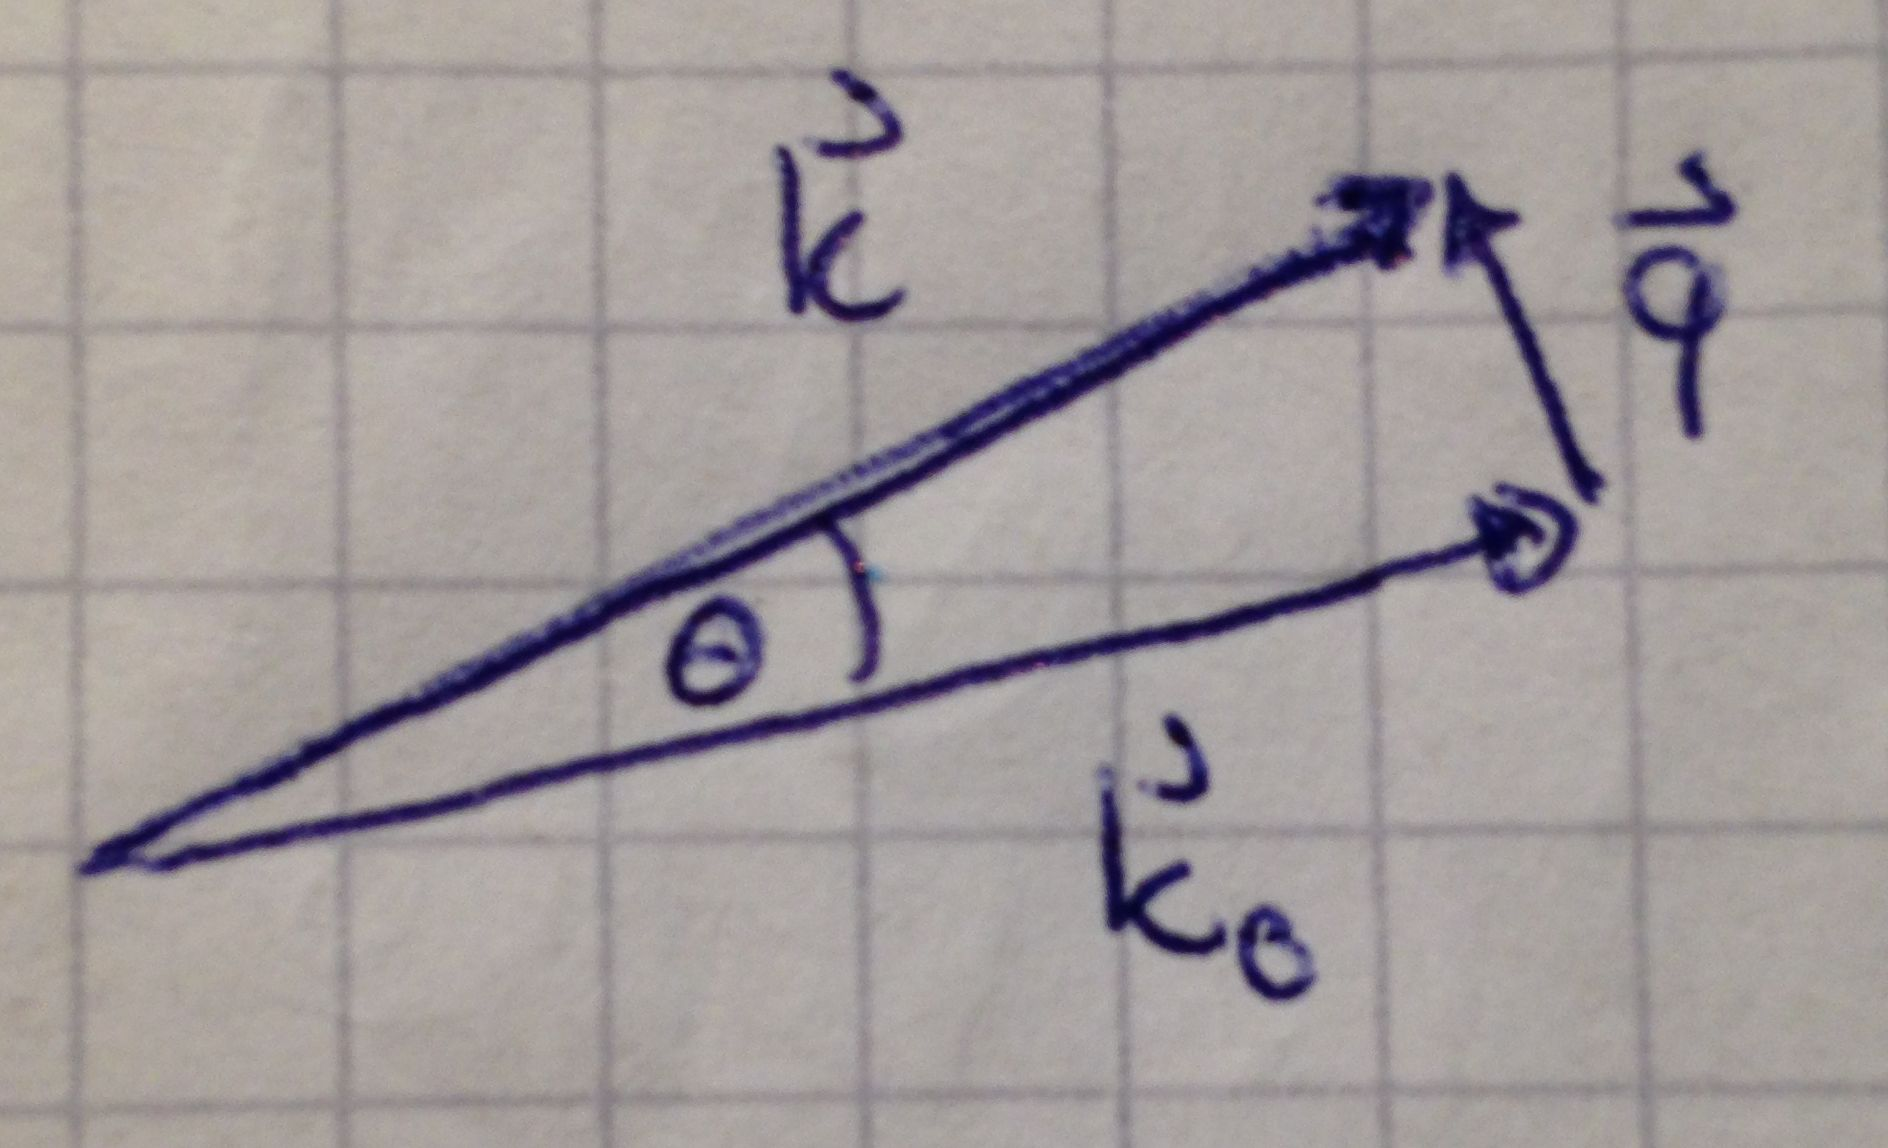
\includegraphics[width=5cm]{Born_Naeherung2}
	\end{minipage}
		
	Born-Näherung für Streuamplitude:
		\begin{empheq}[box=\boxed]{align*}
			f^{(1)} (\theta, \phi) &= -\frac{m}{2 \pi \hbar^2} 
			\int \diff^3 r' ~V(\vec{r}\,') e^{-i \vec{q} \vec{r}}
		\end{empheq}
		\begin{align*}
			f^{(1)} &= -\frac{m}{2 \pi \hbar^2}  \braket{\vec{k}| V | \vec{k}_0}
			& &V \text{ ist Wechselwirkung}
		\end{align*}
	Born-Näherung (1.Ordung der Born-Reihe) der Streuamplitude ist die Fouriertransformierte des Streupotentials.
	
	Impulsübertragung: \marginpar{12.11.2015}
		\begin{align*}
			\vec{q} &= \vec{k} - \vec{k}_0 
			= k (\vec{e}_r - \vec{e}_z)
		\end{align*}
	Wobei $k = |k| = |k_0|$

%	\begin{figure*} [h]
%		\begin{center}
%			\includegraphics[width=8cm]{Annaherung_harte_Kugel3}
%		\end{center}
%	\end{figure*} %dieses Bild hab ich nicht
	
	Born-Näherung für Streuamplitude
		\begin{empheq}[box=\boxed]{align*}
			f^{(1)}(\theta, \phi) =
			-\frac{m}{2 \pi \hbar} 
			\int \diff^3 r' ~V(\vec{r}\,') e^{-i \vec{q} \cdot \vec{r}}
		\end{empheq} 
		\begin{align*}
			``f^{(1)} = -\frac{m}{2 \pi \hbar} 
			\braket{ \vec{k} | V | \vec{k}_0}\text{''}
		\end{align*}
	Streuamplitude ist in Born-Näherung die ``Fouriertransformierte'' des Streupotetials.
	
	Annahme: Kugelsymmetrisches Streupotential:
		\begin{empheq}[box=\boxed]{align*}
			\vec{q}^2 &= (\vec{k} - \vec{k}_0)^2 
			= k^2 \left( 1 - \frac{2 \vec{k} \vec{k}_0}{k^2}
			+ 1 \right)	
			= 2 k^2 (1- \cos \theta) \\
			&= 4 k^2 \sin^2 \frac{\theta}{2}
		\end{empheq}
	wobei $k^2 = |\vec{k}| |\vec{k}_0|$
	
	Setze $\vec{q} = 2 k \sin \frac{\theta}{2}$ in Born-Näherung ein:
		\begin{align*}
			\int \diff^3 r ~V(\vec{r}\,') e^{-i \vec{q} \vec{r}}
			&= 2 \pi \int_{-\infty}^{\infty} \diff r' 
			~r'^2 V(r') 
			\underbrace{\int_{-1}^1 \diff \cos \theta 
			e^{-iqr \cos \theta}}_{\substack{*}} \\
			\left(
			*: \int_{-1}^1 \diff t ~e^{-iqr t} \right.
			\left. 
				- \frac{1}{iqr} e^{-iqrt}
			\right|_{-1}^1
			&= 
				\left. \frac{2}{qr} \sin (qr)
			\right) \\
			\int \diff^3 r ~V(\vec{r}\,') e^{-i \vec{q} \vec{r}}
			&= \frac{4 \pi}{q} \int_{0}^{\infty}
			\diff r' ~r' V(r') \sin (qr')
		\end{align*}
	Streuamplitude: \marginpar{beim zweiten bruch steht noch ein q irgendwie drunter}
		\begin{empheq}[box=\boxed]{align*}
			f^{(1)} (\theta, \phi) = f^{(1)}(\theta)
			= -\frac{2m}{\hbar^2} \frac{1}{2 k q \sin \frac{\theta}{2}} 
			\int_0^{\infty} \diff r' ~r' V(r') \sin (qr')
		\end{empheq}
	Streuamplitude in Born-Näherung für rotationssymmetrische Wechselwirkung.
	
	Optisches Theorem:
		\begin{align*}
			\mathrm{Im} f(\theta = 0) &= \frac{k}{4 \pi} \sigma
			& &\text{Problem: } f^{(1)} \text{ ist reell!}
		\end{align*}
	Die Born-Näherung verletzt das optische Theorem.
	Unzuverlässig bei kleinen $\theta$. Kann nur ``funktionieren'' weg von Vorwärtsentwicklung.
	
	``Gültigkeitsbereich'' (2 Fälle):
		\begin{itemize}
			\item niedrige Energie ($kR \ll 1$):
			$| \int_0^\infty \diff r ~r V(r)|
			\ll \frac{\hbar^2}{2m}$
			\item hohe Energien ($kR \gg 1$):
			$ | \int_0^\infty \diff r ~V(r)| 
			\gg \frac{\hbar^2 k}{2m}$ 
			+ nur für $\theta > 0$
		\end{itemize}
	Beispiel: Yukawa-Potential: 
		\begin{align*}
			V(r) &= \frac{g^2}{4 \pi} \frac{e^{-\mu r}}{r}
			& &\text{Reichweite } R \sim \frac{1}{\mu} \\
			f^{(1)} (\theta) 
			&= - \frac{2m}{\hbar^2} \frac{1}{2 k \sin \left(\frac{\theta}{2}\right)} 
			\int_0^\infty \diff r' ~r' V(r')
			\sin \left(2 k \sin \frac{\theta}{r} r'\right) \\
			&= - \frac{g^2}{4 \pi} \frac{m}{\hbar k \sin \frac{\theta}{2}}
			\int_0^\infty \diff r' ~e^{-\mu r'} 
			\sin \left(2 k \sin \frac{\theta}{2} r' \right)
		\end{align*}
	2 fache partielle Integration:
		\begin{align*}
			f^{(1)}(\theta) 
			&= - \frac{g^2}{4 \pi} \frac{2m}{\hbar^2}
			\frac{1}{\mu^2 +  4 k^2 \sin^2 \frac{\theta}{2}}
			& \mu \rightarrow 0 
			&\Rightarrow \text{ Coulombpotential} \\
			\text{mit } \frac{g^2}{4 \pi} 
			&= Z_1 Z_2 \alpha \hbar c 
			& \text{und } k^2 &= \frac{2mE}{\hbar^2}
		\end{align*}
	und $Z_1$ ist Ladung von Teilen, $Z_2$ ist Ladung von Streuzentrum.
		\begin{empheq}[box=\boxed]{align*}
			\left( \frac{\diff \sigma}{\diff \Omega} \right)^{(1)} 
			&= | f^{(1)}_{\text{Coulomb}}|^2
			= \left(
				\frac{Z_1 Z_2 \alpha \hbar c}{4 E}
			\right)^2
			\frac{1}{\sin^4 \left(\frac{\theta}{2} \right)}
		\end{empheq}
	Dies ist die \underline{Rutherfordstreuung}.
	
	Wir haben ``Glück'', da
		\begin{align*}
			\underset{r \rightarrow \infty}{\lim} r ~V(r) \neq 0
		\end{align*}
	exakte Coulombamplitude unterswcheidet sich von Born-Näherung in diesem Fall nur durch eine Phase.
		\begin{align*}
			f^{\text{exakt}}_{\text{Coulomb}} (\theta) 
			&= -\frac{Z_1 Z_2 \alpha \hbar c}{4 E \sin^2 \frac{\theta}{2}} 
			\exp \left[ 2 i \sigma_0 - 
			2 i \frac{Z_1 Z_2 \alpha \hbar c}{4 E} k 
			\ln \left(\sin^2 \frac{\theta}{2} \right)
			\right] \\
			\text{Streuphase }: \sigma 
			&= \sum_\ell \sigma_\ell 
			= \frac{4 \pi}{k^2} \sum_\ell (2 \ell + 1) \sin^2 \delta_\ell
		\end{align*}
	Born-Näherung für Streuphasen $\delta_\ell$: Einlaufendes Teilen (vgl. harte Kugel)
		\begin{align*}
			e^{i \vec{k_0} \vec{r}\,'} 
			&= \sum_\ell \sqrt{4 \pi (2 \ell + 1)} 
			i^\ell j_\ell (kr') Y_{\ell 0} (\theta') \\
			e^{-i \vec{k} \vec{r}} 
			&= \sum_\ell \sum_{m = -\ell}^\ell
			4 \pi (-i)^\ell j_\ell (kr') Y_{\ell m} (\theta, \phi) Y^*_{\ell m} (\theta', \phi')
		\end{align*}
	Nebenbemerkung:
		\begin{align*}
			\sum_m Y_{\ell m} (\theta, \phi) Y^*_{\ell m} (\theta', \phi') 
			&= \frac{2 \ell + 1}{4 \pi} P_\ell (\cos \sphericalangle (\vec{r},\vec{r}\,'))
		\end{align*}
		\begin{align*}
			\Rightarrow \int \diff \Omega' 
			e^{i(\vec{k}-\vec{k}_0) \vec{r}\,'} 
			&= 4 \pi \sum_{\ell=0}^\infty (2\ell + 1)
			P_\ell (\cos \theta) j_\ell^2 (kr') \\
			f^{(1)} (\theta) 
			&= -\frac{m}{2 \pi \hbar^2} 
			\int \diff^3 r' V(r') e^{i(\vec{k}-\vec{k}_0)\vec{r}} \\
			&= - \frac{2 m}{\hbar^2}
			\int \limits_0^r \diff r' ~r'^2 V(r') 
			\sum_{\ell = 0}^\infty j_\ell^2 (k r') 
			(2 \ell + 1) P_\ell (\cos \theta) 
		\end{align*}
	Vergleich mit:
		\begin{align*}
			f^{(1)}(\theta) 
			&= \frac{1}{k} \sum_{\ell=0}^{\infty} (2\ell + 1)
			\underline{e^{i\delta_\ell} \sin \delta_\ell} P_\ell (\cos \theta) \\
			\Rightarrow e^{i\delta_\ell} \sin \delta_\ell
			&= - \frac{k 2 m}{\hbar^2} 
			\int \limits_0^\infty \diff r ~V(r) 
			[r ~j_\ell(kr)]^2
		\end{align*}
	Streuphasen für rotationssymmetrisches Potential in Born-Näherung:
		\begin{empheq}[box=\boxed]{align*}
			\mathrm{Re} (\underline{ e^{i\delta_\ell} \sin \delta_\ell})
			&\approx \delta_\ell
			\leftarrow \delta_\ell \text{ klein für Born-Näherung} \\
			&\approx -\frac{2m}{k \hbar^2}
			\int \limits_0^\infty \diff r ~V(r) 
			~[(kr)j_\ell(kr)]^2
		\end{empheq}
	%Kap 3
	\section{Systeme mit mehr als 2 ``Teilchen''}
	\section{Systeme mit mehr als 2 ``Teilchen''}
	\subsection{Das Pauliprinzip}
		Beispiel: Atom mit $N$ Elektronen $e^-$.
			\begin{align*}
				H &= \sum_{i=1}^N H^{(i)} ,& 
				H^{(i)} &= - \frac{\vec{p}^{(i)2}}{2m} + V(\vec{r}^{(i)}) 
			\end{align*}
		Hierbei wurde die $e^- -e^- -$ Wechselwirkung ungerechtfertigerweise vernachlässigt.
		
		stationäre Schrödinger Gleichung:
			\begin{align*}
				H \phi_{\vec{\alpha}} &= E_{\vec{\alpha}} \phi_{\vec{\alpha}} 
				&\text{mit } \phi_{\vec{\alpha}} &= \prod_{i=1}^N \phi_{\alpha_i} \\
				H^{(i)} \phi_{\alpha_i} &= E_{\alpha_i} \phi_{\alpha_i} 
				&E_{\vec{\alpha}} &= \sum_{i=1}^N E_{\alpha_i} \\
				\alpha_i &= (n_i, \ell_i , m_i) 
				&\text{oder mit } &(\vec{p}+e \vec{A})^2 
				\text{ Pauligleichung} \\
				\alpha_i &= (n_i, j_i, m_i , \ell_i ,(s_i))
			\end{align*}
		und $s_i = \frac{1}{2}$
			\begin{align*}
				n_i &: \text{Hauptquantenzahlen} \\
				j_i &: \text{Drehimpulsquantenzahl } ( \text{Gesamtdrehimpuls } \vec{J}_i = \vec{L}_i + \vec{S}_i) \\
				m_i &: \text{Magnetsiche Quantenzahl } (\vec{J}_i)_z \ket{\phi_{\alpha_i}} = m_i \ket{\phi_{\alpha_i}} \\
				\ell_i &: \text{Bahndrehimpulsquantenzahl}
			\end{align*}
		Grundzustand:
			\begin{align*}
				\alpha_i = (1, \frac{1}{2}, \pm \frac{1}{2}, 0)
			\end{align*}
		Pauliverbot (Ausschließungsprinzip):
		
		Jeder Einteilchenzustand $\phi_\alpha$ kann höchstens mit einem $e^-$ besetzt sein. \\
		Pauliprinzip (Dirac + Heisenberg):
		
		Die Wellenfunktion eines Systems von Elektronen ist total antisymmetrisch. \\
		Definiere Permutation
			\begin{align*}
				\pi &\in S_N ,~ \sigma (\pi) = \mathrm{sign}(\pi) \in \{+1, -1\} \\	
				\sigma &: \text{Signum der Permutation}\\
				\sigma (\pi) &=
				\left\{
					\begin{aligned}
						&+1 \text{ gerade} ,& &\text{gerade Anzahl von paarweise VerIRGENDWAS} \\
						& & &\text{führt } (1,2,3, \ldots) \text{ in } \prod (1,2,3,\ldots) \text{ über}\\
						&-1 \text{ ungerade} ,& &\text{ungerade Anzahl} (\ldots)
					\end{aligned}
				\right.
			\end{align*}
		\underline{Antisymmetrisierungsoperator}:
			\begin{align*}
				A &= \frac{1}{\sqrt{N!}} \sum_{\pi \in S_N} \sigma (\pi) \cdot \pi 
				&\Rightarrow (A \phi) (\vec{r}_1, \ldots, \vec{r}_N) 
				&= \frac{1}{\sqrt{N!}} \sum_{\pi \in S_N} \sigma(\pi)
				\phi \left((\vec{r}_{\pi(1)}, \vec{r}_{\pi(2)}, \ldots ,\vec{r}_{\pi(N)}\right)   
			\end{align*}
			\begin{align*}
				A \phi_{\vec{\alpha}} (\vec{r}_1, \ldots, \vec{r}_N)
				&= \frac{1}{\sqrt{N!}} 
				\det
				\begin{pmatrix}
					\phi_{\alpha_1}(\vec{r}_1, \sigma_1) & \cdots & \phi_{\alpha_1}(\vec{r}_N, \sigma_N) \\
					\vdots & \ddots & \vdots\\
					\phi_{\alpha_N}(\vec{r}_1, \sigma_1) & \cdots & \phi_{\alpha_N}(\vec{r}_N, \sigma_N)
				\end{pmatrix}
			\end{align*}
	Wdh: 1-Teilchen Wellenfunktionen (Fermionen)\marginpar{16.11.2015}
		\begin{align*}
			\phi_{\alpha_1}(\vec{r}_1, \sigma_1), \ldots, \phi_{\alpha_N}(\vec{r}_N, \sigma_N)
		\end{align*}
	Das $\sigma$ zeigt Spin an.
		\begin{align*}
			\phi_{\alpha_1} &= 
			\begin{pmatrix}
				\phi_{+, \alpha_1 (\vec{r}_1)} \\
				\phi_{-, \alpha_1 (\vec{r}_1)}
			\end{pmatrix}
		\end{align*}
	hier kommt irgendwas von flavour, was uns nur verwirren kann.
	
	Fermionische Gesamtwellenfunktion ist total antisymmetrisch
		\begin{align*}
			\text{Spin } &\in \left\{ 0, \frac{1}{2}, 1 , \frac{3}{2}, 2 , \ldots \right\} 
			& (\text{Pauliprinzip})
		\end{align*}
	wobei $0, 1 , 2$ Bosonen sind und $\frac{1}{2}, \frac{3}{2}$ Fermionen sind.
	
	Antisymmmetris... siehe oben
	
	Beispiel: $N = 2$
		\begin{align*}
			\psi_{\alpha_1 \alpha_2} (\vec{r}_1, \sigma_1; \vec{r}_2, \sigma_2)
			&= A \overbrace{(\phi_{\alpha_1 \alpha_2} (\vec{r}_1, \sigma_1; \vec{r}_2, \sigma_2))}^{\mathclap{\phi_{\alpha_1} (\vec{r}_1, \sigma_1) \cdot \phi_{\alpha_2}(\vec{r}_2, \sigma_2)}} \\
			&= \frac{1}{\sqrt{2}}
			\left(\phi_{\alpha_1} (\vec{r}_1, \sigma_1) \cdot \phi_{\alpha_2}(\vec{r}_2, \sigma_2)
			- \phi_{\alpha_1} (\vec{r}_2, \sigma_2) \cdot \phi_{\alpha_2}(\vec{r}_1, \sigma_1)\right)
		\end{align*}
	Antisymmetrische Gesamtwellenfunktion von $2 e^-$ im Zustand $\alpha_1$ und $\alpha_2$ 
		\begin{align*}
			\alpha_1 &= \alpha_2 \Rightarrow \psi = 0 ~(\text{Pauliverbot})
		\end{align*}
		\begin{align*}
			\text{Bosonen } \longleftrightarrow& 
			\text{ ganzzahliger Spin (Beispiel: Photon)} \\
			&\Rightarrow \text{ Total symmetrische Wellenfunktion}\\
			\text{Fermionen } \longleftrightarrow& 
			\text{ halbzahliger Spin (Beispiel: Elektron)} \\
			&\Rightarrow \text{ Total antisymmetrische Wellenfunktion}
		\end{align*}

	\subsection{Das Heliumatom}
	\begin{align*}
		H = \left(\frac{\vec{p}^{(1)2}}{2m} - \frac{Z \alpha \hbar c}{r_1}\right)
		+ \left(\frac{\vec{p}^{(2)2}}{2m} - \frac{Z \alpha \hbar c}{r_2}\right)
		+ \frac{\alpha \hbar c}{|\vec{r}_1 - \vec{r}_2|}
	\end{align*}
Hierbei wurde die Spin Wechselwirkung vernachlässigt (warum auch immer), die beiden Terme in den Klammern sind $H^{(1)}$ und $H^{(2)}$, der Letzte ist $V_e(\vec{r}_1, \vec{r}_2)$, wir setzen $Z=2$ für 2 Protonen (obwohl $Z$ trotzdem immer wieder vorkommen wird).
	\begin{align*}
		\alpha_1 &= (n_1, \ell_1, m_1) & &\text{(weil Spin Ww vernachlässigt)} \\
		\vec{S} &= \vec{S}^{(1)} + \vec{S}^{(2)} & &\text{(Gesamtspin)}
	\end{align*}
	\begin{align*}
		\text{Gesamtspin }1& & \left(\vec{S}^2 \ket{\psi} = S(S+1) \hbar^2 \ket{\psi} \right) \\
		\ket{S, S_z} &= \ket{1 ,1} = \ket{+~+} \\
		\ket{S, S_z} &= \ket{1, -1} = \ket{-~-} \\
		\ket{S, S_z} &= \ket{1, 0} = \frac{1}{\sqrt{2}} \left( \ket{+~-} + \ket{-~+} \right)
	\end{align*}
Spinwellenfunktion ist symmetrsich. \\
$\Rightarrow$ Bahnwellenfunktion ist antisymmetrisch (\underline{Ortho-Helium})
	\begin{align*}
		\text{Gesamtspin }0& \\
		\ket{0 , 0} &= \frac{1}{\sqrt{2}} \left( \ket{+~-} - \ket{-~+} \right)
	\end{align*}
Spinwellenfunktion ist antisymmetrisch $\Rightarrow$ Bahnwellenfunktion ist symmetrisch (Para-Helium)

Gesamtwellenfunktion
	\begin{align*}
		\Psi(\vec{r}_1, \sigma_1 ; \vec{r}_2, \sigma_2) 
		&= \Psi(\vec{r}_1, \vec{r}_2) \chi (\sigma_1, \sigma_2) \\
		S = 1: \psi (\vec{r}_1, \vec{r}_2) &=
		\frac{1}{\sqrt{2}} 
		\left( \psi^{(1)} (\vec{r}_1) \psi^{(2)} (\vec{r}_2) 
		- \psi^{(1)}(\vec{r}_2) \psi^{(2)} (\vec{r}_1) \right) \\
		S = 0: \psi (\vec{r}_1, \vec{r}_2) &=
		\frac{1}{\sqrt{2}} 
		\left( \psi^{(1)} (\vec{r}_1) \psi^{(2)} (\vec{r}_2) 
		+ \psi^{(1)}(\vec{r}_2) \psi^{(2)} (\vec{r}_1) \right)
	\end{align*}
	\begin{align*}
		\text{mit } H^{(1)} \psi^{(1)} (\vec{r}) &= E^{(1)} \psi^{(1)} (\vec{r}) \\
		&\left(\text{bei Vernachlässigung von } V_e (\vec{r}_1, \vec{r}_2) \right) \\
		E_{\alpha_1 \alpha_2} &= E_{n_1 n_2} \approx 
		- \frac{1}{2} m c^2 Z^2 \alpha^2 
		\left( \frac{1}{n_1^2} + \frac{1}{n_2^2} \right)
	\end{align*}	
	\begin{align*}
		S = 0 &\Rightarrow n_1 = n_2 \text{ ist möglich immer.} \\
		S = 1 &\Rightarrow n_1 = n_2 \text{ für } n_1= 1
		(\Rightarrow \ell_1 = m_1 = 0 \Rightarrow \alpha_1 = \alpha_2) 
		\text{ ist verboten}
	\end{align*}
Grundzustandsenergie: 
	\begin{align*}
		E_{11} &\approx 2 E_1 = 2 Z^2 E_1 ( \overbrace{H}^{\mathclap{\text{Wasserstoff}}}) 
		= 8 E_1 (H) \approx -108,8 eV \\
		&( S= 0 (\text{Parahelium})) 
	\end{align*}
\underline{1.Anregung:}
	\begin{align*}
		E_{12} &\approx \left(1 + \frac{1}{4}\right) Z^2 E_1 (H) = 5 E_1(H) \approx -68,0 eV \\
		&(\text{möglich für Ortho- und Parahelium})
	\end{align*}
Betrachte $V_e(\vec{r}_1, \vec{r}_2) = \frac{\alpha \hbar c}{|\vec{r}_1 - \vec{r}_2|}$ als Störung
	
Grundzustand:
	\begin{align*}
		\Delta E_{11} &=
		\braket{ 1, 0, 0 ; 1, 0, 0| V_e | 1, 0 , 0; 1, 0 ,0 } & 
		&\text{also so:}\bra{n_1, \ell_1, m_1; n , \ell, m} \text{ usw.}\\
		&= \int \diff^3r_1 \diff^3r_2 |\psi_{100} (\vec{r}_1)|^2 |\psi_{100}(\vec{r}_2)|^2
		\frac{\alpha \hbar c}{|\vec{r}_1 - \vec{r}_2|} \\
		&\psi_{100} (\vec{r}) = \frac{1}{\sqrt{\pi}} 
		\left(\frac{Z}{a_B}\right)^{\frac{3}{2}} e^{-\frac{Zr}{a_B}}\\
		&= \frac{5}{4} \frac{Z \alpha \hbar c}{2 a_B} 
		= \frac{5}{4} Z \underbrace{\frac{mc\alpha^2}{2}}_{\mathclap{-E_1(H)}} 
		\approx 34 eV
	\end{align*}
	\begin{align*}
		E_{11} &= -108,8 eV + 34 eV + \ldots \approx - 74,8 eV \\
		\text{Experiment} &: -78,975eV (\text{Parahelium Grundzustand}) \\
		\Delta E_{1n} &\text{ mit } n>1 \\
		\psi (\vec{r}_1, \vec{r}_2) 
		&= \frac{1}{\sqrt{2}}
		\left( \psi_{100}(\vec{r}_1) \psi_{n \ell m}(\vec{r}_2) 
		\pm \psi_{100}(\vec{r}_2) \psi_{n \ell m} (\vec{r}_1) \right)
	\end{align*}
Das $``+''$ für Para-, das $``-''$ für Ortho-Helium.
	\begin{align*}
		\Delta E_{11} &=
		\int \diff^3 r_1 \diff^3 r_2 |\psi_{100} (\vec{r}_1)|^2 |\psi_{n \ell m} (\vec{r}_2)|^2
		\frac{2}{2} \frac{\alpha \hbar c}{|\vec{r}_1 - \vec{r}_2|} \\
		&\pm \int \diff^3 r_1 \diff^3 r_2 \psi_{100}^* (\vec{r}_1) \psi_{n \ell m}^* (\vec{r}_2)
		\psi_{100} (\vec{r}_2) \psi_{n \ell m} (\vec{r}_1)
		\frac{\alpha \hbar c}{|\vec{r}_1 - \vec{r}_2|} \\
		&= K_{n \ell} \pm A_{n \ell}
	\end{align*}
	\begin{align*}
		K_{n \ell} \geq 0 &: \text{Coulombenergie} & 
		&\text{Betrachte } n=2 \Rightarrow \ell = 0 \text{ oder } \ell = 1\\
		A_{n \ell} \geq 0 &: \text{Austauschenergie} \\
		\Delta E_{12} &= K_{2 \ell} \pm A_{2 \ell} &
		&\begin{aligned}
			&+ \text{ für Parahelium } 2^1 P, 2^1 S \\
			&- \text{ für Orthohelium } 2^3 P, 2^3 S
		\end{aligned}
	\end{align*}
	\begin{align*}
		K_{21} &= \frac{Z}{2} \alpha^2 m c^2 \frac{118}{243} \approx 13,2 eV \\
		A_{21} &= \frac{Z}{2} \alpha^2 m c^2 \frac{7}{12} \approx 15,9 eV
		,& A_{20} &= \frac{Z}{2} \alpha^2 m c^2 \frac{32}{729} \approx 0,6 eV
	\end{align*}
$\Rightarrow$ Ortho-Parahelium Energienieveauaufspaltung wegen des Pauli-Prinzips (Selbst wenn wir Spin Wechselwirkung in $H$ vernachlässigen) 

Spektroskompische Notation $n^{2 S + 1} \cdot L_J$

wobei $n=1,2,3$ und $L_J = S, P, D$ für $L=0, 1, 2$

	\begin{figure*} [h]
		\begin{center}
				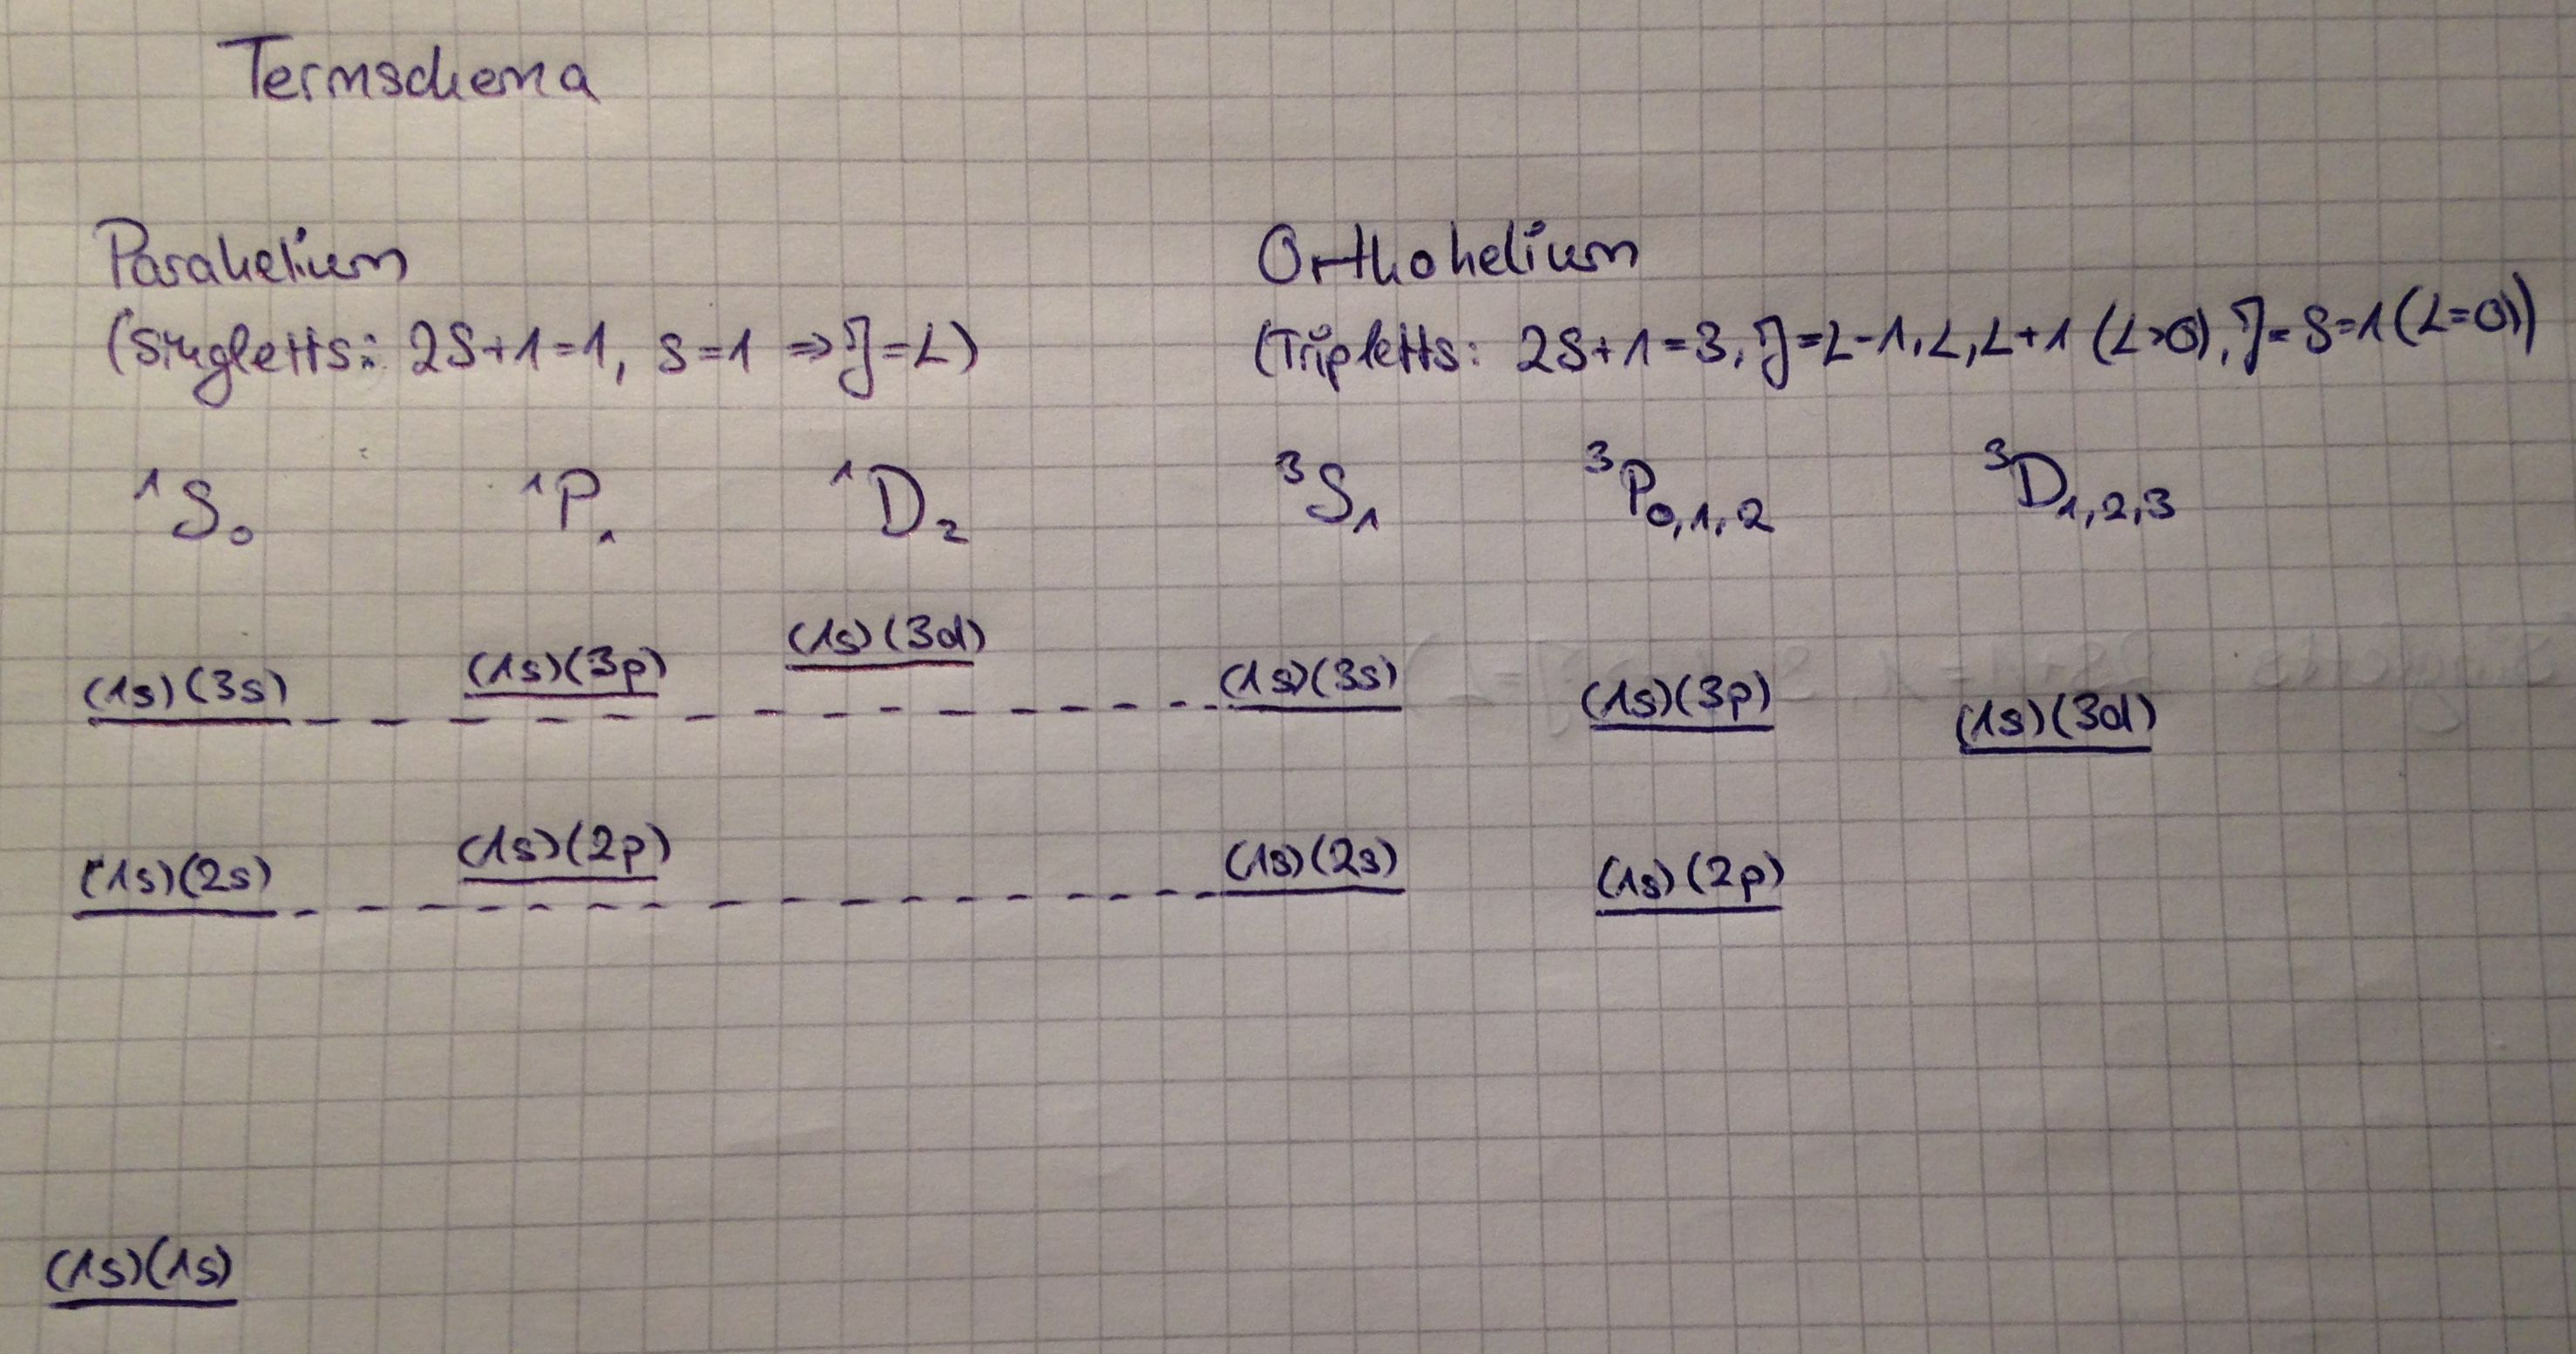
\includegraphics[width=\textwidth]{Termschema}
		\end{center}
	\end{figure*}

\subsection{Ritz-Variationsverfahren}
	\begin{align*}	
	\braket{\psi | H | \psi} &= \int \limits_\alpha\!\!\!\!\!\!\!\!\!\;\sum
	\braket{\psi | \alpha} E_\alpha \braket{\alpha | \psi} \\
	&\geq E_0 \int \limits_\alpha\!\!\!\!\!\!\!\!\!\;\sum |\braket{\psi | \alpha}|^2 
	= E_0 \braket{\psi | \psi}
	\end{align*}
	\begin{empheq}[box=\boxed]{align*}
		\Rightarrow \braket{\psi | H | \psi} &= E_0 \text{ für } \braket{\psi | \psi} = 1 \\
		\text{bzw. } E_0 &= \underset{\psi}{\mathrm{inf}} 
		\frac{\braket{\psi | H | \psi}}{\braket{\psi| \psi}}
	\end{empheq}
Betrachte eine nicht unbedingt normierte Testwellenfunktion, welche abhängt von kontinuierlichen Parametern $b_i$
	\begin{align*}
		\ket{\psi (b_1, \ldots, b_N)}& \\
		E(b_1, \ldots, b_N) &= 
		\frac{\braket{\psi (b_1, \ldots, b_N)|H|\psi (b_1, \ldots, b_N)}}{\braket{\psi (b_1, \ldots, b_N)|\psi (b_1, \ldots, b_N)}} \\
		E_{\text{min}} &= \underset{\{b_1, \ldots, b_N\}}{\mathrm{min}}
		E(b_1, \ldots, b_N) \geq E_0
	\end{align*}
Heliumatom
	\begin{align*}
		\text{Ansatz: } \psi_{100}(\vec{r}, Z^*)
		&= \frac{1}{\sqrt{\pi}} \left(\frac{Z^*}{a_B}\right)^{\frac{3}{2}} e^{-\frac{Z^* r}{a_B}}
	\end{align*}
Dies ist motiviert durch Wasserstoffwellenfunktion, aber mit ``effektiver'' Kernladung 
$Z* < Z = 2$, da das andere Elektron die Kernladung teilweise abschirmt.
	\marginpar{19.11.15}
	\begin{align*}
		H &= \underbrace{\frac{\vec{p}^{(1)2}}{2m} - \frac{Z^* \alpha \hbar c}{r_1}}_{\mathclap{*}}
		\underbrace{- \frac{(Z-Z^*)\alpha \hbar c}{r_1}}_{\mathclap{**}} \\
		&\underbrace{+ \frac{\vec{p}^{(2)2}}{2m} - \frac{Z^* \alpha \hbar c}{r_2}}_{\mathclap{*}}
		\underbrace{- \frac{(Z-Z^*)\alpha \hbar c}{r_2}}_{\mathclap{**}} \\
		&\underbrace{+ \frac{\alpha \hbar c}{|\vec{r}_1 - \vec{r}_2|}}_{\mathclap{V_e(\vec{r}_1, \vec{r}_2)}} + (\text{Spinabhängiger Term})
	\end{align*}
	\begin{align*}
		\braket{\psi_{100}(Z^*) | H | \psi_{100}(Z*)} 
		&= \underbrace{2E_1(Z^*)}_{\mathclap{*}} 
		\underbrace{- 2 \alpha \hbar c (Z - Z*) \erw{\frac{1}{r}}_{10}}_{\mathclap{**}}
	\end{align*}
Wobei * Grundzustandsenergie von $H$-Problem mit Kernladung $Z^* e$ und die $10$ beim Erwartungswert sind die $n \ell$ für Wasserstoff.
	\begin{align*}
		E_1(Z*) &= - \frac{1}{2} (Z^*)^2 m c^2 \alpha^2 ,&
		\erw{\frac{1}{r}}_{10} &= \frac{Z*}{a_B} \\
		\Rightarrow \braket{\psi | H | \psi} &= 
		-\frac{1}{2} m c^2 \alpha^2 
		\left( 2 (Z^*)^2 - 4 (Z^* - Z)Z^* \frac{5}{4} Z^* \right)\\
		&= \frac{1}{2} m c^2 \alpha^2 
		\left( 2 (Z^*)^2 - 8Z^* + \frac{5}{4} Z^* \right) & &\text{hier sind irgendwo Rechenfehler}
	\end{align*}
	\begin{align*}
		\frac{\partial \left(
			\frac{\braket{\psi | H | \psi}}{\braket{\psi | \psi}}
			\right)}{\partial Z^*}
		&= \frac{1}{2} m c^2 \alpha^2 \left( 4 Z^* - \frac{27}{4} \right) = 0 \\
		& \Rightarrow \boxed{Z^* = \frac{27}{16}} \\
		E_{\text{min}} &= - m c^2 \alpha^2 (Z- (Z - Z^*))^2 = -77,5eV
	\end{align*}
Zum Vergleich 

Störungstheorie, alles in $eV$ \\
	\begin{tabular}{c | c | c | c | c | c | c | c | c}
		Ordung & 0 & 1 & 2 & 3 & 4 & 5 & ``Exakt'' & Experiment \\
		\hline
		E & -108,832 & -74,822 & - 79,112 & -78,998 & -78,999 & -79,003 & -79,005 & -78,975
	\end{tabular}
Das Experiment weicht wegen der Wechselwirkungsterme, die wir vernachlässigt haben, ab.
	
	Ritz mit 2 Parametern $\psi \sim (1 + b_2 r) e^{-\frac{Z^* r}{a_B}} \leadsto -78,6eV$

\subsection{Atombau}

	\begin{tabular}{c c c c c c}
		$n$ & $\ell$ & Bezeichnung & Maximalzahl von $e^-$ & Besetzungsreihenfole & $Z$ \\
		\hline
		1 & 0 & $1s$ & 2 & 1 & 1-2 \\
		\hline
		2 & 0 & $2s$ & 2 & 2 & 3-4 \\
		  & 1 & $2p$ & 6 & 3 & 5-10 \\
		\hline
		3 & 0 & $3s$ & 2 & 4 & 11-12 \\
		  & 1 & $3p$ & 6 & 5 & 13-18 \\
		  & 2 & $3d$ & 10 & 6 & 19-30 \\
		\hline
		4 & 0 & $4s$ & 2 & 6 & 19-30 \\
		  & 1 & $4p$ & 6 & 7 & 31-36 \\
		  & 2 & $4d$ & 10 & 8 & 37-48 \\
		  & 3 & $4f$ & 14 & 10 & 55-80 \\
	\end{tabular}
	\subsection{Hartrei-Fock-Approximation}
	\begin{align*}
		H &= \sum_i H^{(i)} + \sum_{i<j} V_{ij}
	\end{align*}
$H^{(i)}$ ist Hamiltonopertor für nicht mit anderen (ununterscheidbaren) Fermionen wechselwirkendes Fermion $i$.
	\begin{align*}
		H \psi_0 &= E_0 \psi_0 
		&\text{mit } E_0 &= \underset{\braket{\psi | \psi} = 1}{\mathrm{min}} \braket{\psi | H | \psi}
	\end{align*}
Grundzustandsenergie

Approximation:
	\begin{align*}
		\psi (1, \ldots, N) 
		&= \frac{1}{\sqrt{N!}} \det 
		\begin{pmatrix}
		\phi_{1}(1) & \cdots & \phi_{1}(N) \\
		\vdots & \ddots & \vdots\\
		\phi_{N}(1) & \cdots & \phi_{N}(N)
		\end{pmatrix} 
	\end{align*}
In der Matrix jeweils in der Klammer stehen Position, Spin etc. und unten sind die Quantenzahlen.
	\begin{align*}
		\phi_i (k) &=
		\underbrace{\phi_i (\vec{r}_k)}_{\mathclap{\text{Bahnwellenfunktion}}}
		\overbrace{\chi_i (\sigma_k)}^{\mathclap{\text{Spinwellenfunktion}}} \\
		\text{Nebenbedingung } &\braket{\phi_i | \phi_j} = \delta_{ij}
	\end{align*}
Dies schränkt nicht die Algemeinheit ein.

Normierung:
	\begin{align*}
		1 &= \braket{\psi | \psi} = \prod_i \braket{\phi_i | \phi_i} 
		& \phi_i &\mapsto \lambda_i \phi_i \\
		1 &= \braket{\psi | \psi} 
		&\mapsto \prod_i |\lambda_i|^2 \braket{\phi_i | \phi_i} &= \prod_i |\lambda_i|^2
		&\Rightarrow 1 &= \prod_i |\lambda_i|^2 = 1 
	\end{align*}
Andere Normierung ist... 
	\subsection{Die Born-Oppenheimer Approximation}
	Beispiel: 2-atomige Moleküle $H C\ell, CO, H_2, O_2, \ldots$ 
		\begin{align*}
			m &: \text{Reduzierte Masse} ,& m_e &: \text{Elektronmasse} \\
			a &: \text{räumliche Ausdehnung } \sim 10^{-10}\mathrm{m} \\
			m_{\text{proton}} &\approx 1830 m_{e^-} &
			m_{H_2} &\approx \frac{m_{\text{proton}} \cdot m_{\text{proton}}}{m_{\text{proton}} + m_{\text{proton}}} \approx \frac{m_{\text{proton}}}{2} \gg m_e
		\end{align*}	
	(hier nummerierung mit (a) usw., weiß ich noch nicht, wie ich das machen werde)
	\begin{enumerate}[(a)]
	\item \underline{Energieniveaus}
			\begin{align*}
				E_{e^-} \sim \frac{p^2}{2m_e} \approx \frac{\hbar^2}{m_e a^2}
			\end{align*}
		(dabei wurde das Virialtheorem genutzt)
		
		Emittiertes Photon bei elektronischem Übergang:
			\begin{align*}
				E_\gamma &= \hbar \omega = c \hbar k = \frac{2 \pi \hbar c}{\lambda}
				\sim E_{e^-} \\
				\lambda &\approx \frac{2 \pi \hbar c}{E_{e^-}} \approx \frac{1200 e\mathrm{V} \cdot \mathrm{nm}}{E_{e^-}} ,&
				\text{denn } 197 \mathrm{nm}\cdot e\mathrm{V} &= \hbar c
			\end{align*}
		Typisch: $E_\gamma = 0, 2, \ldots 3 e$V $\Rightarrow \lambda = 400-6000$nm (sichtbar bis infrarot)
	\item \underline{Schwingungsniveaus} (Abstand der Atomkerne)
			\begin{figure*} [h]
				\begin{center}
					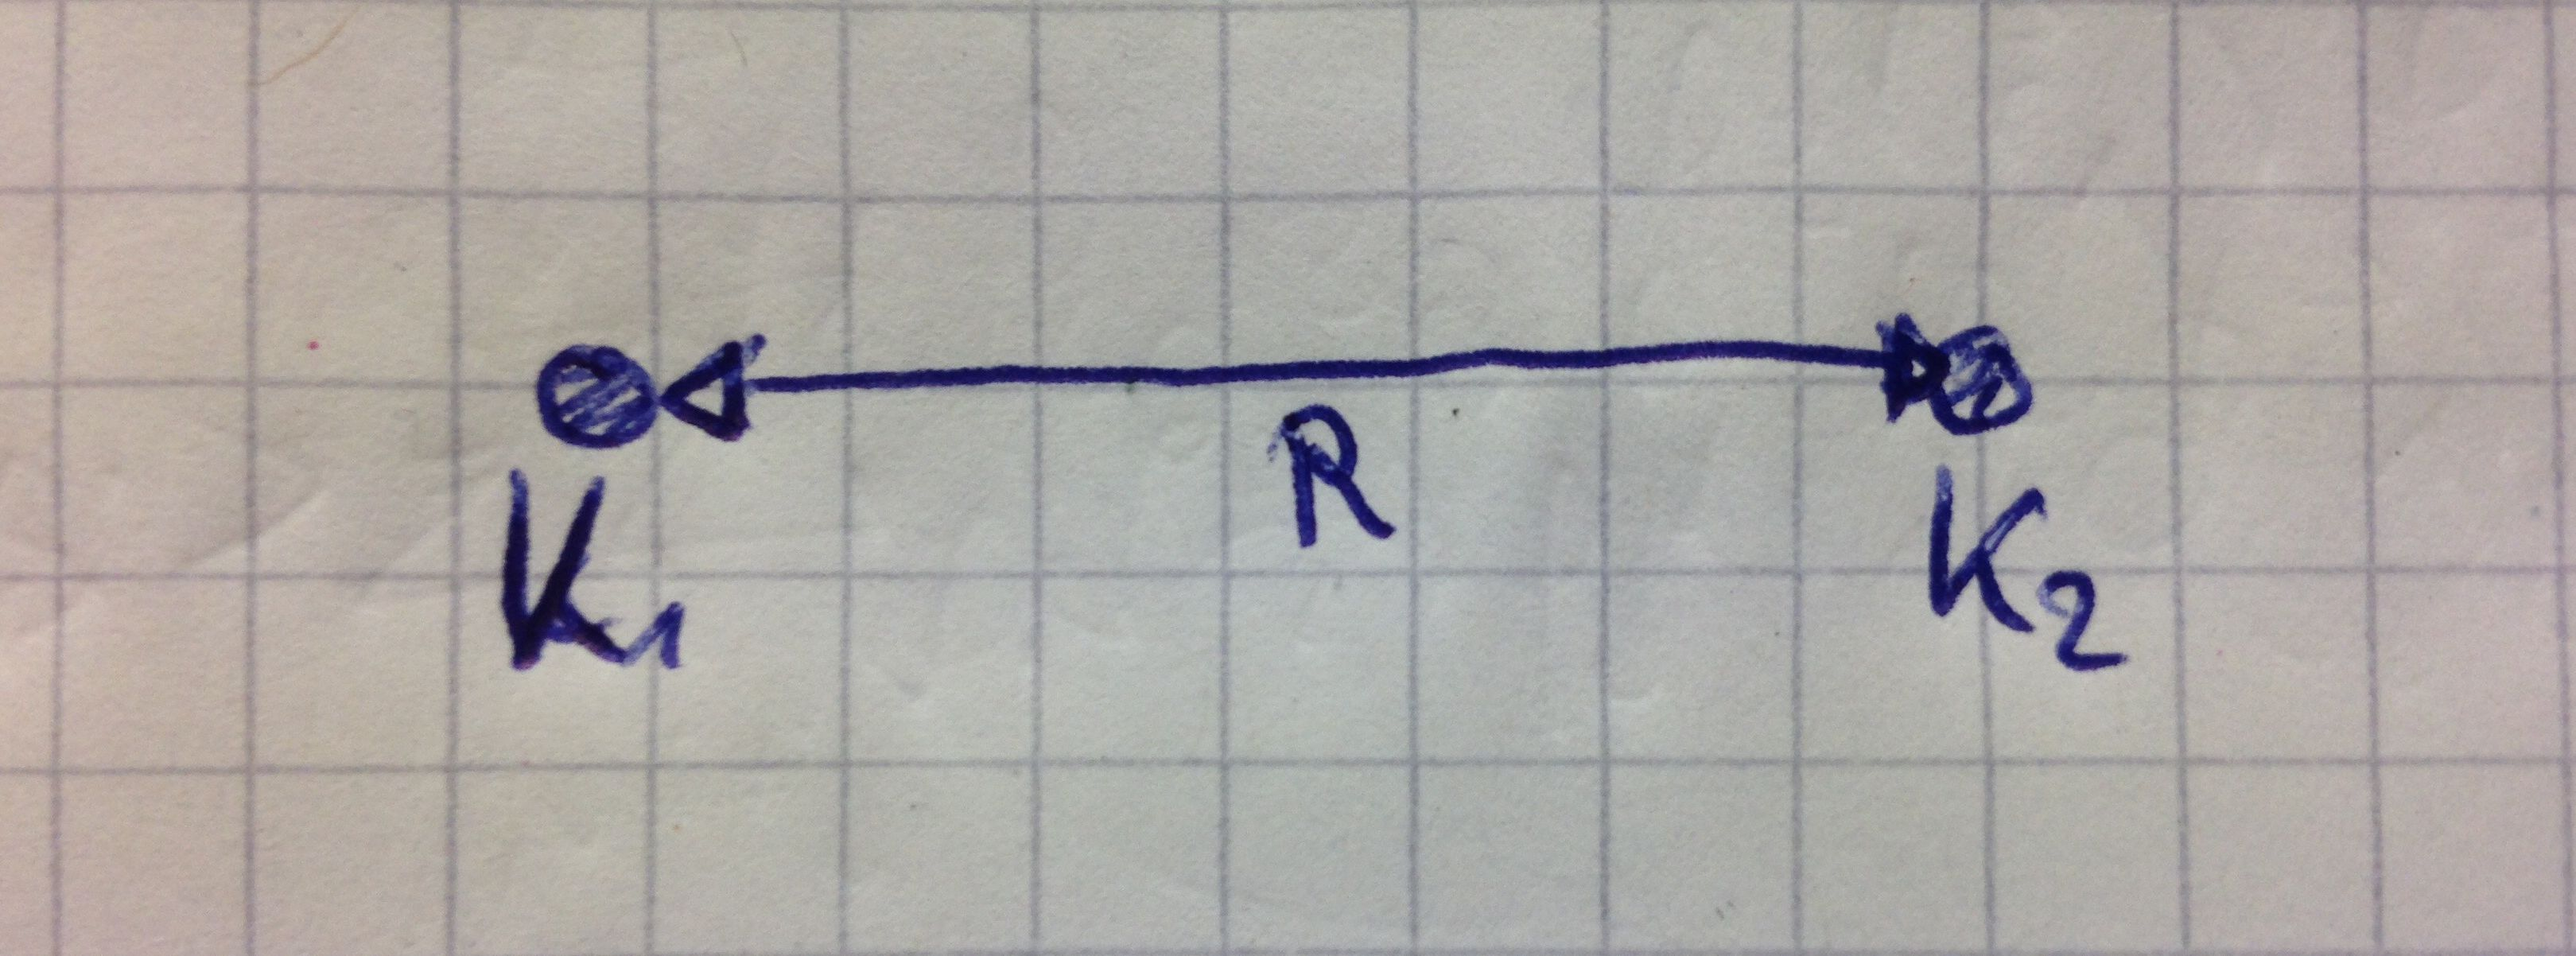
\includegraphics[width=10cm]{Born-Oppenh_Approx1}
				\end{center}
			\end{figure*}
			
		Potenzielle Energie $\U (R)$
			\clearpage
			\begin{figure*} [h]
				\begin{center}
					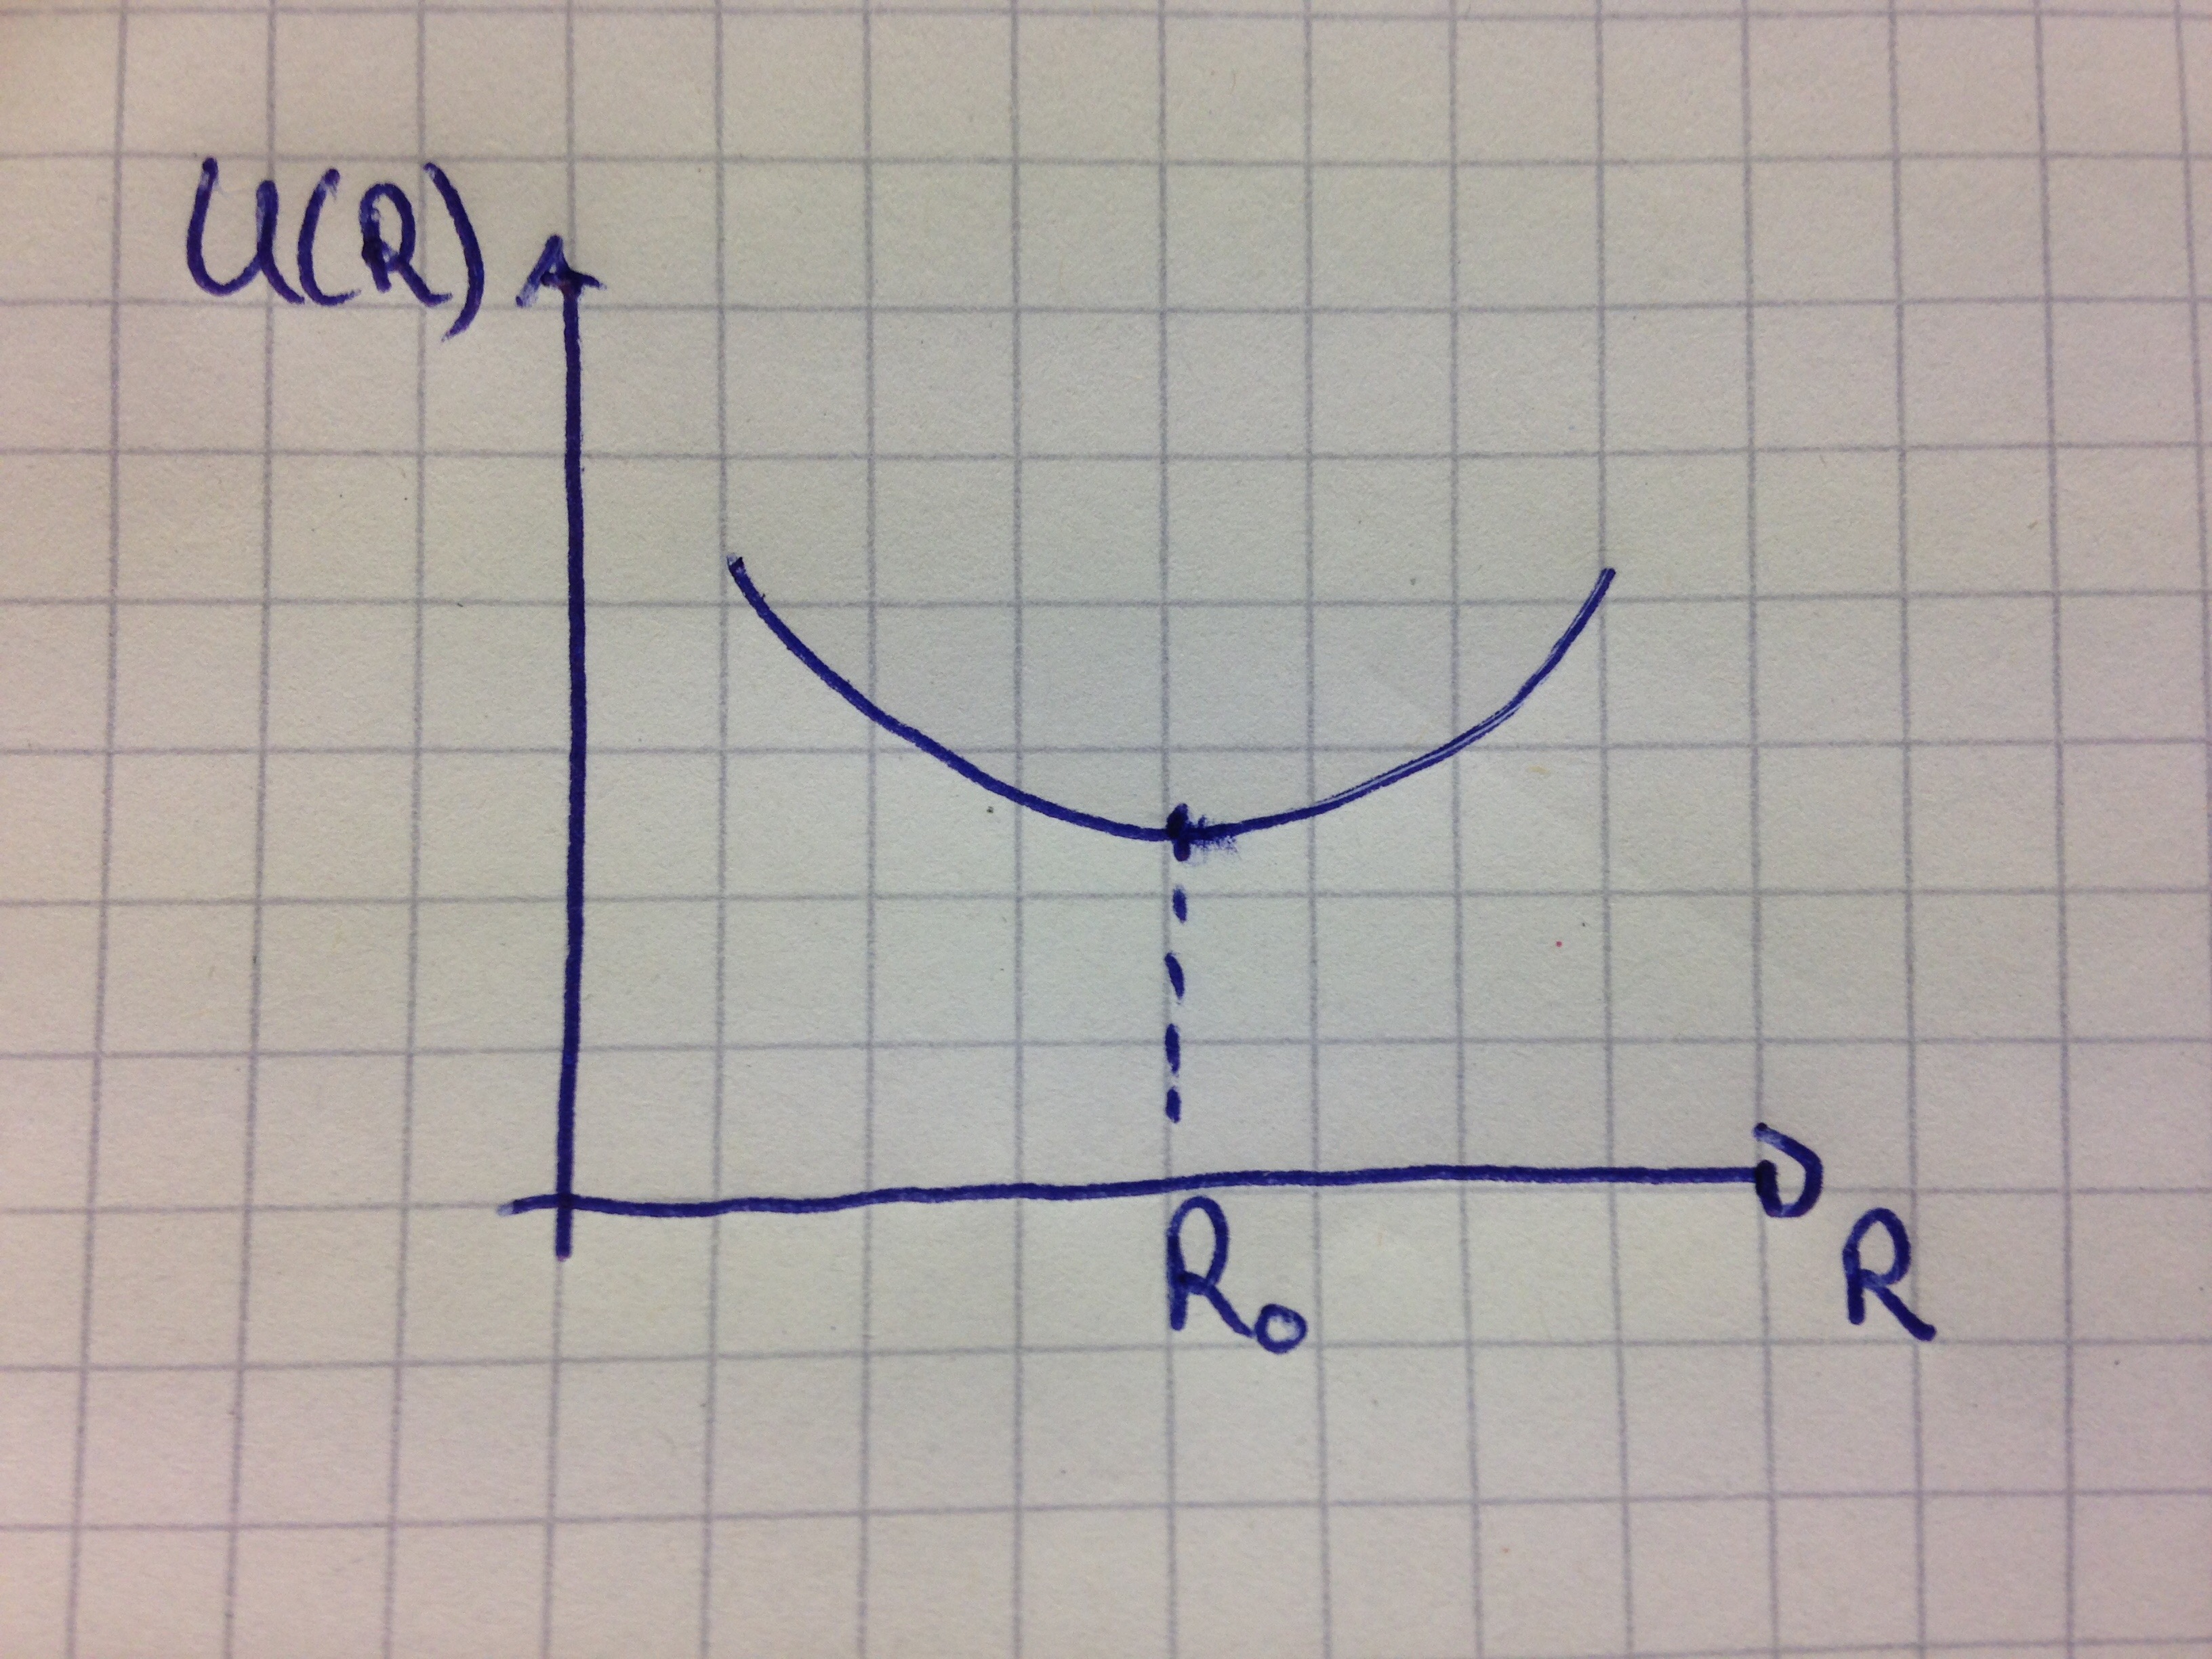
\includegraphics[width=10cm]{Born-Oppenh_Approx2}
				\end{center}
			\end{figure*}
			\begin{align*}
				\U(R) &= const. + \frac{1}{2} m \omega_{\mathrm{vib}}^2 
				\overbrace{(R-R_0)^2}^{\mathclap{< a^2}} \\
				m \omega_{\mathrm{vib}}^2 a^2 &\sim E_{\mathrm{Bindung}} \sim E_{e^-} \\
				E_{\mathrm{vib}} &= \hbar \omega_{\mathrm{vib}} 
				\sim \sqrt{\frac{E_{\mathrm{Bindung}}}{m}} \sqrt{\frac{\hbar^2}{a^2}}
				\sim E_{e^-} \sqrt{\frac{m_e}{m}} \\
				m &\approx 10^4 m_e 
				\Rightarrow E_{\mathrm{vib}} \sim 10^{-2} E_{e^-} 
				\Rightarrow \lambda > 40 \mu \mathrm{m} = 4 \cdot 10^{-3} \mathrm{cm}
			\end{align*}
	\item \underline{Rotationsniveaus}
	
		Trägheitsmoment $I \sim m a^2$
			\begin{align*}
			E_{\mathrm{rot}} &= \frac{L^2}{2 I} 
			= \frac{\hbar^2 \ell (\ell + 1)}{2 I} \sim \frac{\hbar^2}{m a^2}
			\sim \frac{m_e}{m} \cdot E_{e^-} \sim \sqrt{\frac{m_e}{m}} E_{\mathrm{vib}}\\
			&\approx 10^{-4} E_{e^-} \approx 10^{-2} E_{\mathrm{vib}} \\
			\lambda &\approx 0,1 \ldots 1 \mathrm{cm} \\
			&(\omega = 2,45 \mathrm{GHz} \cdot 2 \pi \Rightarrow \lambda \approx 12 \mathrm{cm})
			\end{align*}
		Separation nach Potenz von $\sqrt{\frac{m_e}{m}} \approx \frac{1}{100}$
	\end{enumerate}
	Born-Oppenheimer Näherung:
	
	Elektronische Anregungen beeinflussen kaum die Vibration. Vibrationen beeinflussen kaum den Rotationszustand. 
	$V_{\mathrm{Kern}} \ll V_{e^-}$:
	\begin{enumerate}[1.]
		\item Löse Schrödingergleichung für $e^-$ für gegebenes $R$
		
			Energien (Molekülterme) : $\U_n(R)$
		\item Löse für vorgegebenes $e^-$ Zustand $n$ die Schrödingergleichung: \label{bla}
				\begin{align*}
					\left( - \frac{\hbar^2}{m} \vec{\nabla}_R^2 + \U_n (R)
					\right)	
					\Psi_N (\vec{R}) &= E_N (\vec{R}) \\
					\U_n (R) &\approx const. + \left.\frac{1}{2} \frac{\partial^2}{\partial R^2}
					\right|_{R=R_0} + \ldots = \\
					&= const. + \frac{1}{2} m \omega_{\mathrm{vib}}^2 (R=R_0)^2 
				\end{align*}
			$\Rightarrow$ Schwingungsniveaus: Aufspaltungen: $\mathscr{O} \left(\sqrt{\frac{m_e}{m}}\right)$ unterdrückt
			
			Rotationsmoden: Aufspaltungen $\mathscr{O} \left(\frac{m_e}{m}\right)$
			
		\item Korrigiere $e^-$ Wellenfunktion und $\U_n(R) \curvearrowright \U_{n,N}(R)$ 
			 $\mathscr{O} \left(\frac{m_e}{m}\right)^{\frac{3}{2}}$ 
			 
			 und zurück nach \ref{bla}
	\end{enumerate}
\subsection{Homonukleare Moleküle (Beispiel $H_2$)}
	\begin{figure*} [h]
		\begin{center}
			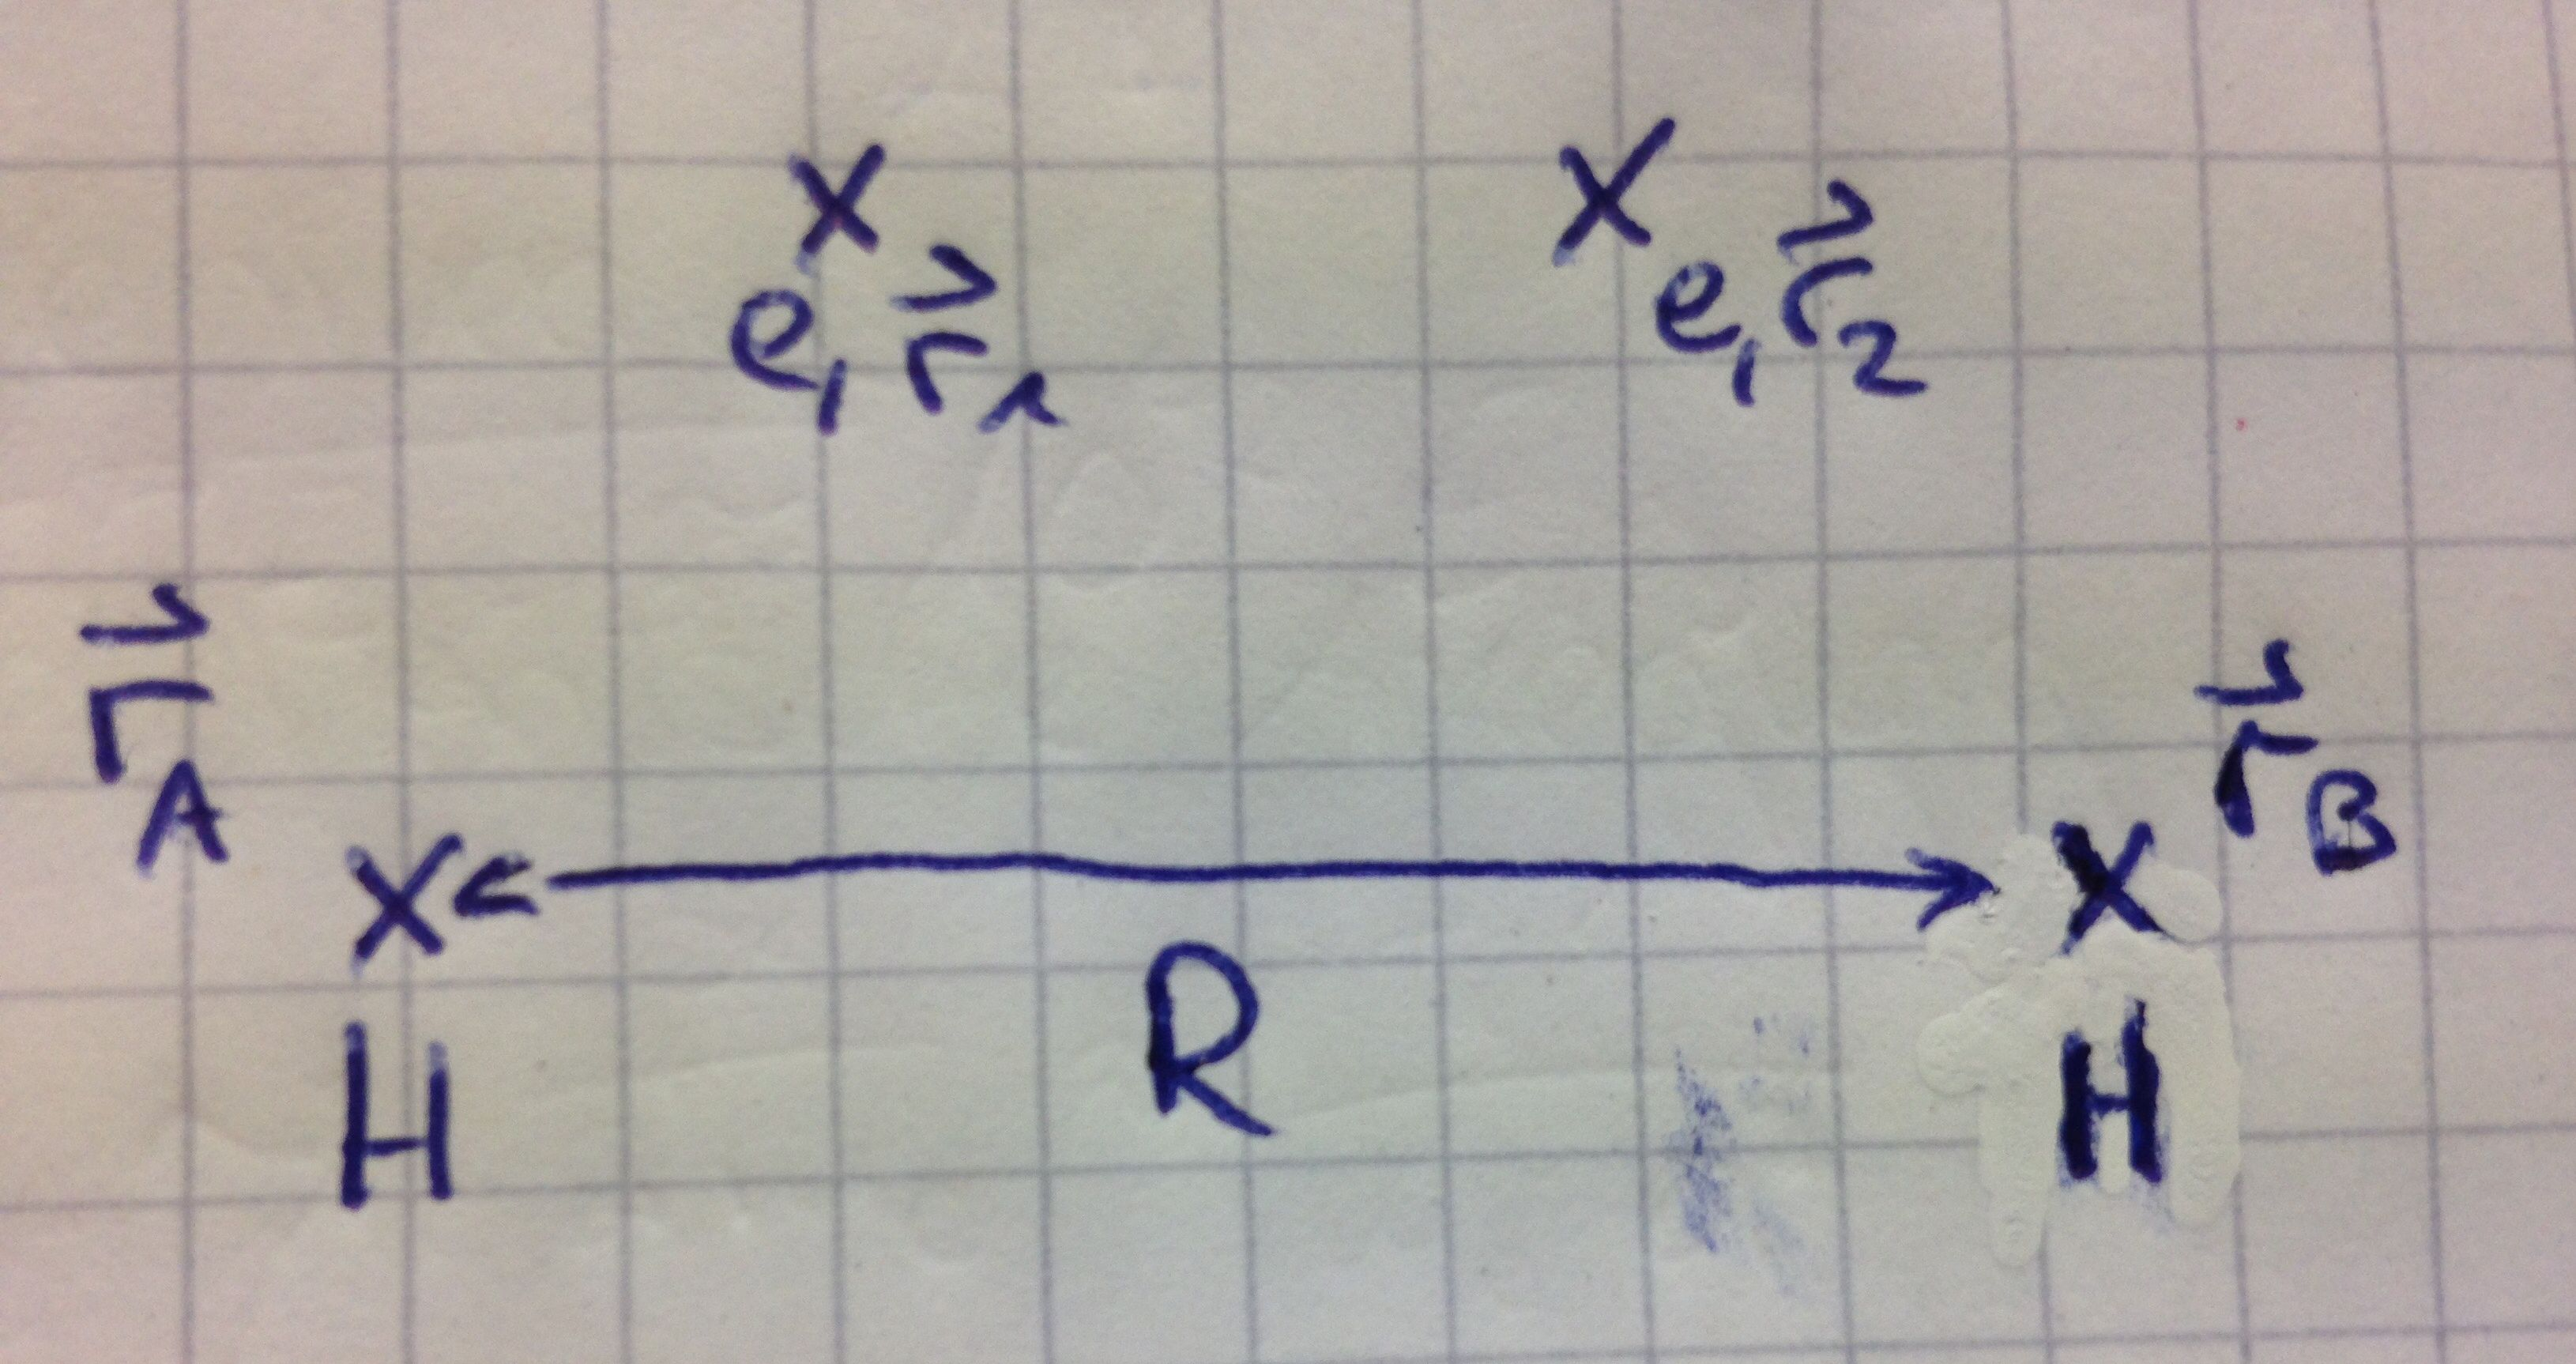
\includegraphics[width=10cm]{Born-Oppenh_Approx3}
		\end{center}
	\end{figure*}
	\subsection{Homonukleare Moleküle (Beispiel $H_2$)}
	\begin{figure*} [h]
		\begin{center}
			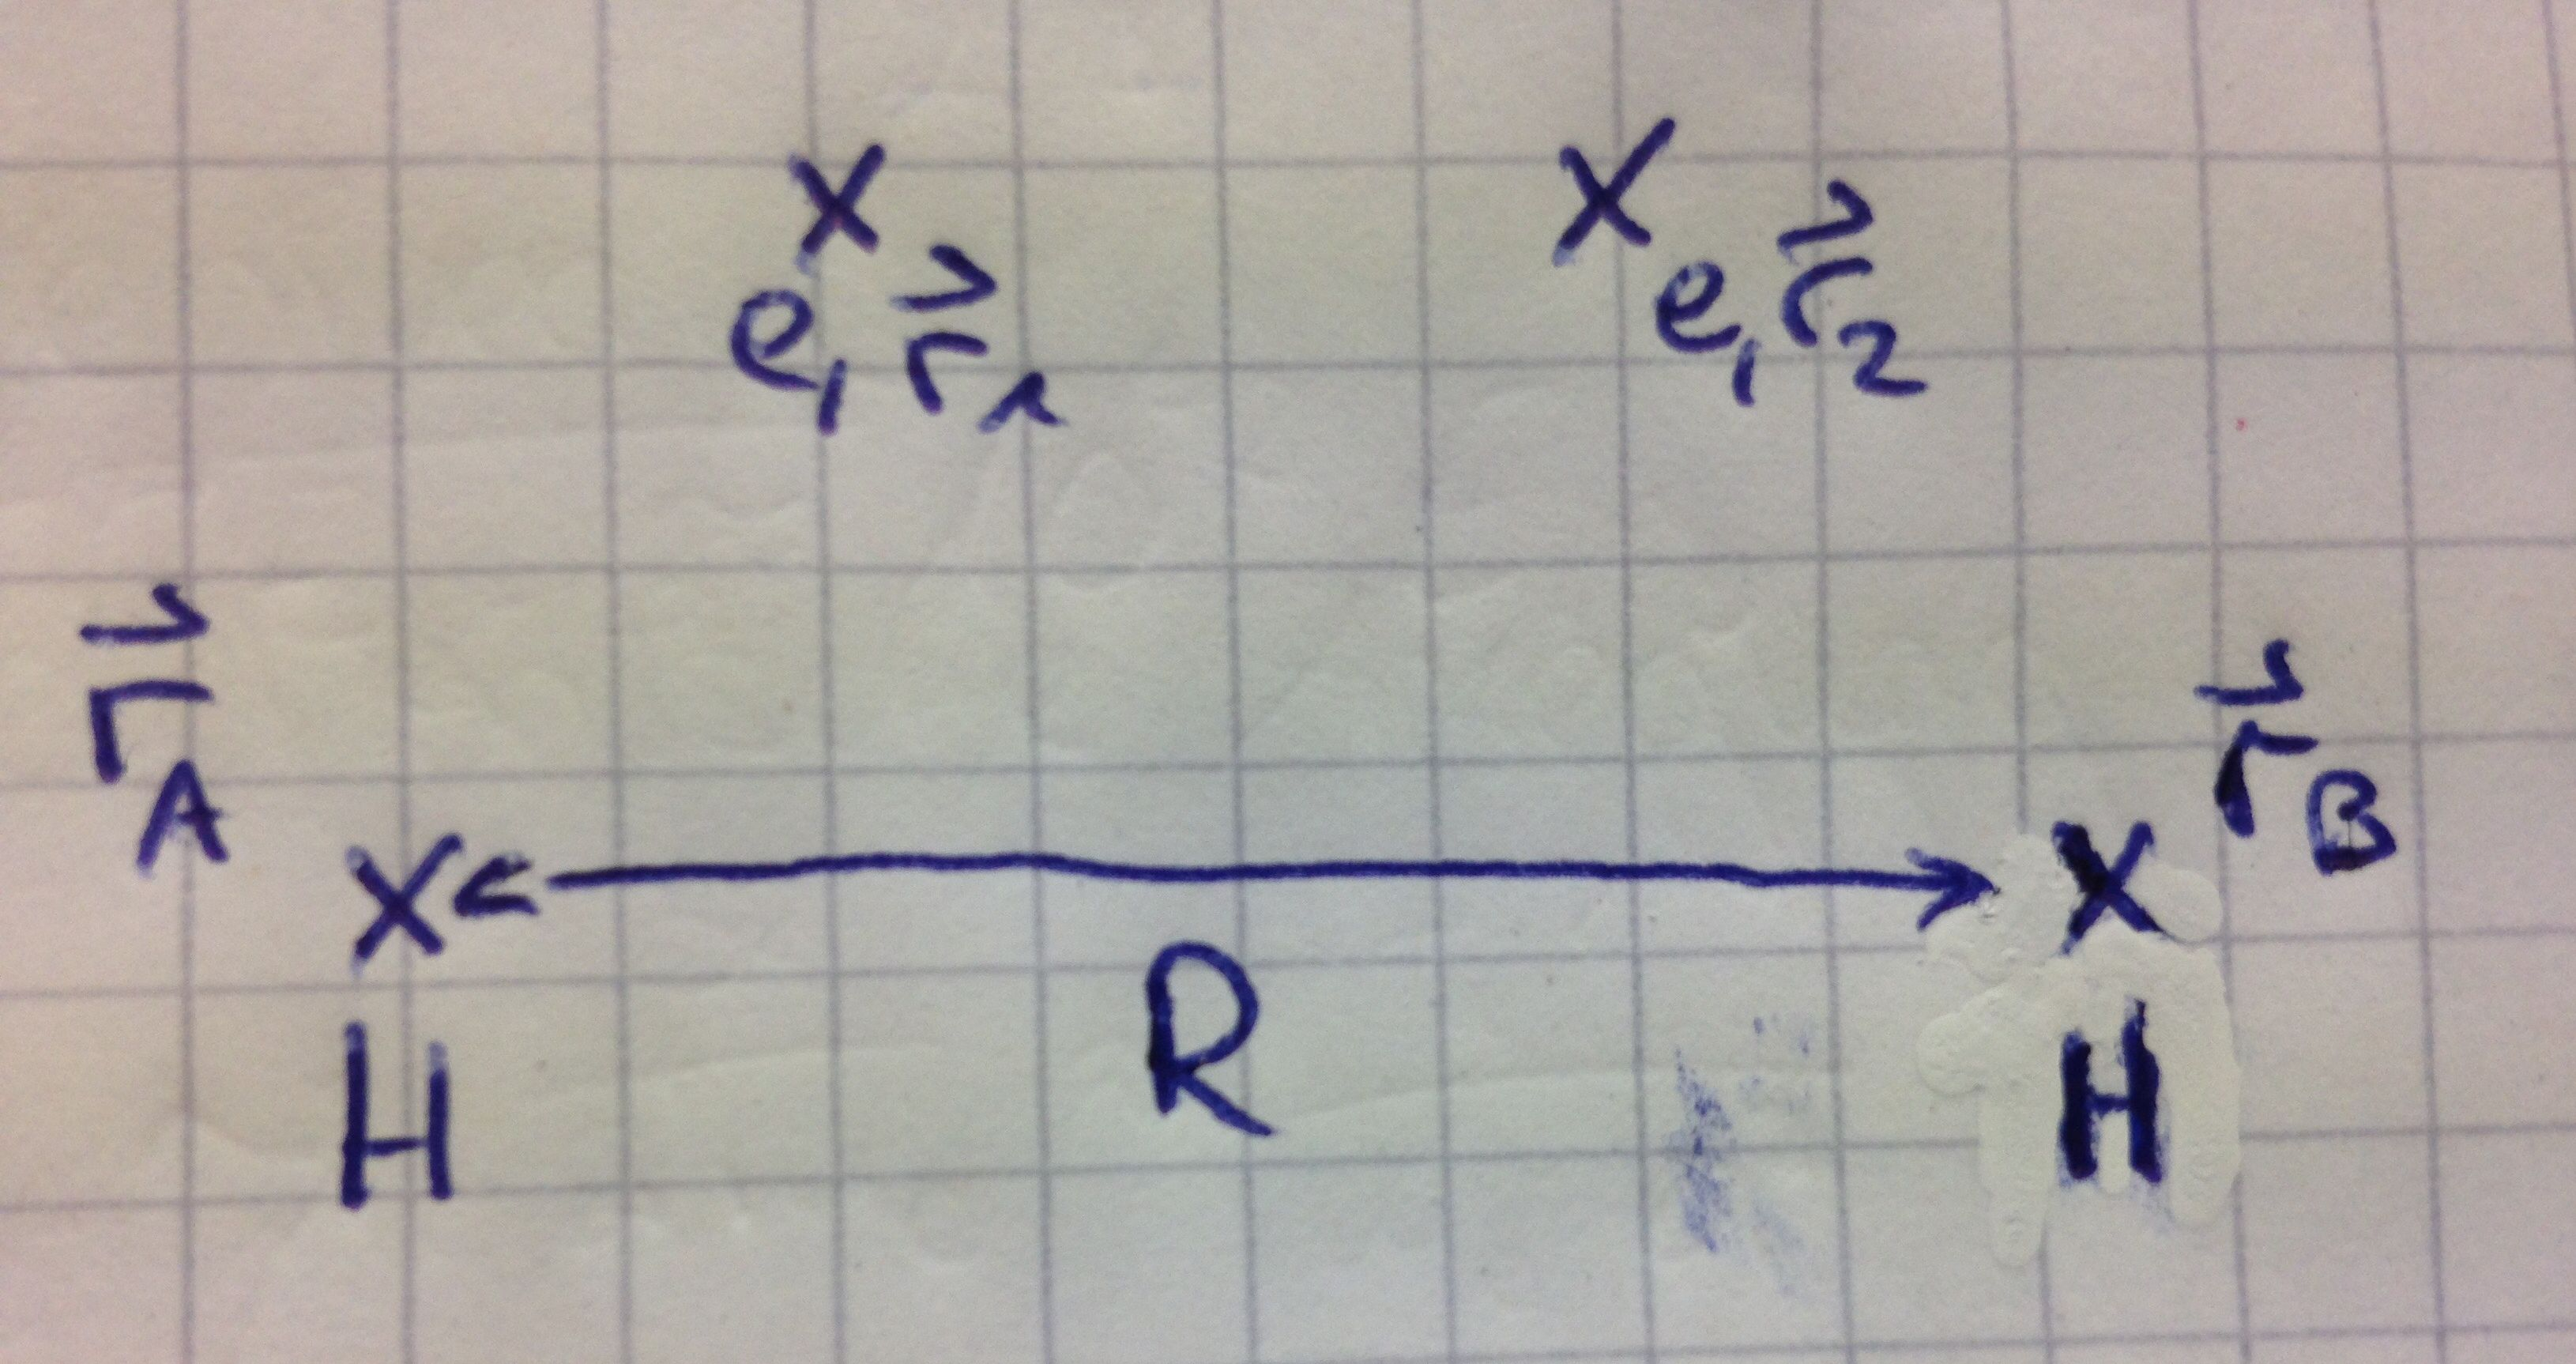
\includegraphics[width=10cm]{Homonukleare_Molekuele1}
		\end{center}
	\end{figure*}
	\begin{align*}
		R = | \vec{r}_A - \vec{r}_B |
	\end{align*}
	\begin{align*}
		R \rightarrow \infty &: \text{Separiert in 2 ``isolierte'' }H \text{-Atome} \\
		R \rightarrow 0 &: He\text{-Wellenfunktion}
	\end{align*}
Rotationssymmetrie gebrochen zu zylindrischer Symmetrie
	\begin{align*}
		C_\infty &\subset \mathscr{O} (3) 
		&\text{Homonuklear } C_{\infty_h} &= C_{\infty_h} \times C_i
	\end{align*}
$C_i$ ist die Parität

$L, J,$etc. keine ``guten'' Quantenzahlen.

Projektionvon $\vec{L}$ auf Molekühlachse $\Lambda$ ist erhalten
	\begin{align*}
		\Lambda &= 0, 1, 2, \ldots ,&
		\Lambda_z &= \pm \Lambda ~(\text{analog zu } m, \text{ aber } m = -\ell, +\ell) \\
		&\left(\Sigma, \Pi, \Delta, \text{etc.}\right)
		& ^{2S + 1}\Lambda &, \text{z.B. } ^3 \Pi ~(\text{Spin-Triplet}) 
	\end{align*}
Weitere Symmetrie: Spiegelung an Ebene
	\begin{figure*} [h]
		\begin{center}
			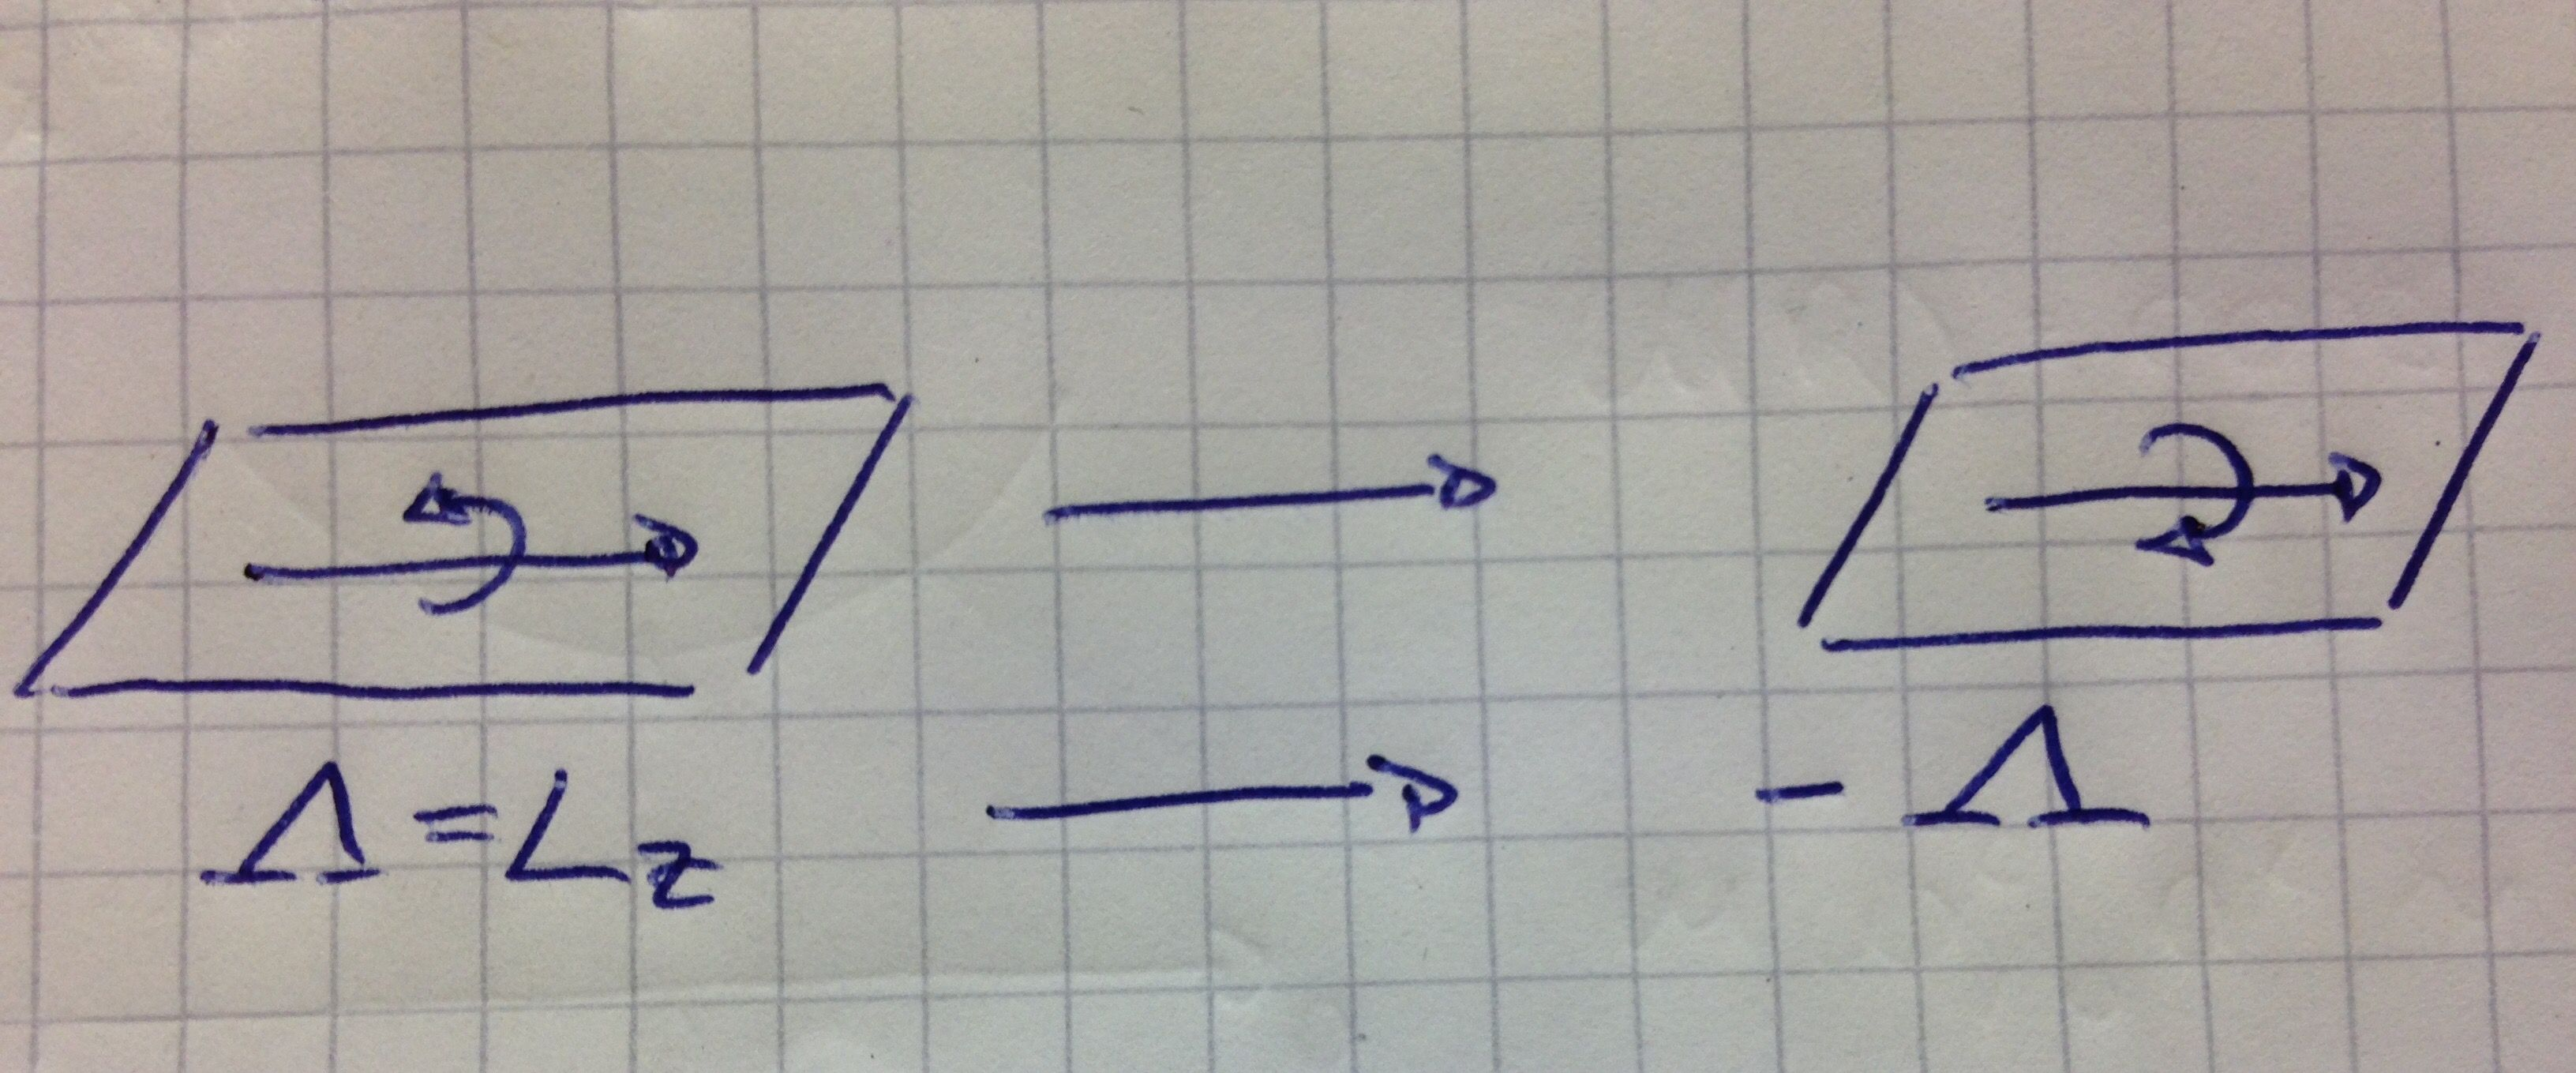
\includegraphics[width=10cm]{Homonukleare_Molekuele2}
		\end{center}
	\end{figure*}
	\begin{align*}
		\Lambda > 0 &: \text{Zustände sind 2-fach entartet. } (\text{analog zu } 2 \ell + 1 \text{ bei Rotationssymmetrie}) \\
		\Lambda = 0 &: \text{Eigenwerte } \sigma_V = + 1, \text{ oder } \sigma_V = -1.\\
		&\curvearrowright \Sigma^+ oder \Sigma^-
	\end{align*}
Homonuklear: Inversion am Mittelpunkt
	
$\Rightarrow$ Parität $\eta = g, u$ 
\\
Molekühlorbits:
	\begin{align*}
		^{2 S + 1}\Sigma_{g, u}^{+ , -} , ^{2 S + 1} \Pi_{g, u}, ^{2 S + 1}\Delta_{g, u}, \ldots
	\end{align*}
Grundzustand: Bahnwellenfunktion 

hat keine Knotetn $\curvearrowright \eta = g, \sigma_V = +$.
\\
Bahnwellenfunktion ist symmetrisch unter
	\begin{align*}
		\vec{r} \rightarrow - \vec{r} &\Rightarrow \text{ Spinwellenfunktion ist antisymmetrisch}\\
		&\Rightarrow S = 0
	\end{align*}
Wir interessieren uns für 	
	\begin{align*}
		^1\Sigma^+, ^1\Sigma^+_g ~(\text{homonuklear})
	\end{align*}
``Ausnahme'':
	\begin{align*}
		O_2 &: ^3\Sigma^-_g & &\text{hier kommen zeichnungen hin, }\\
		NO &: ^2\Pi & &\text{hab aber zu wenig ahnung von Chemielatexzeugsi}
	\end{align*}
	\begin{align*}
		R &\rightarrow 0 : He &\text{Parität } P &\rightarrow \eta = (-)^{S + L}
		&(\vec{r}_i \rightarrow -\vec{r}_i \text{ nicht } \vec{r}_1 \leftrightarrow \vec{r}_2) \\
		\Lambda &= 0 &\Sigma^{(-)^L \cdot \eta} &= \Sigma^{(-)^S}
	\end{align*}
$R \rightarrow 0$ verschiedene $D_{\infty_h}$ Zuständie geben dasselbe $J^{PC}$ (was das auch immer sein möge, ich hab echt keine Ahnung)

	\begin{tabular}{l l}
		He & H$_2$ \\
		$^1S_0$ & $^1\Sigma^+_g$ \\
		$^3S_1$ & $^3\Sigma^-_u$ \\
		$^1P_1$ & $^1\Sigma^+_u, ^1\Pi_u$\\
		$^3P_{0,1,2}$ & $^3\Sigma^-_g, ^3\Pi_g$\\
	\end{tabular}
	
Und hier war noch eine skurile Zeichnung, die keiner verstanden hat ;-)\\

$R \rightarrow \infty$ (2 isolierte $H$-Atome)\marginpar{26.11.15}
	\begin{align*}
		\left.
		\begin{aligned}
			2 \text{ mal } ^2S_{\frac{1}{2}} &\longrightarrow &
			S &= 0 & (\eta &= g) \\
			& & S &= 1 & (\eta &= \mu) 
		\end{aligned}
		\right\}
		\Lambda &= 0 ,~ \sigma_v  = +1
	\end{align*}
Grundzustand für $R \rightarrow \infty$ 
	\begin{align*}
		^1\Sigma^+_g &\text{ oder } ^3\Sigma^+_u
	\end{align*}
	\begin{figure*} [h]
		\begin{center}
			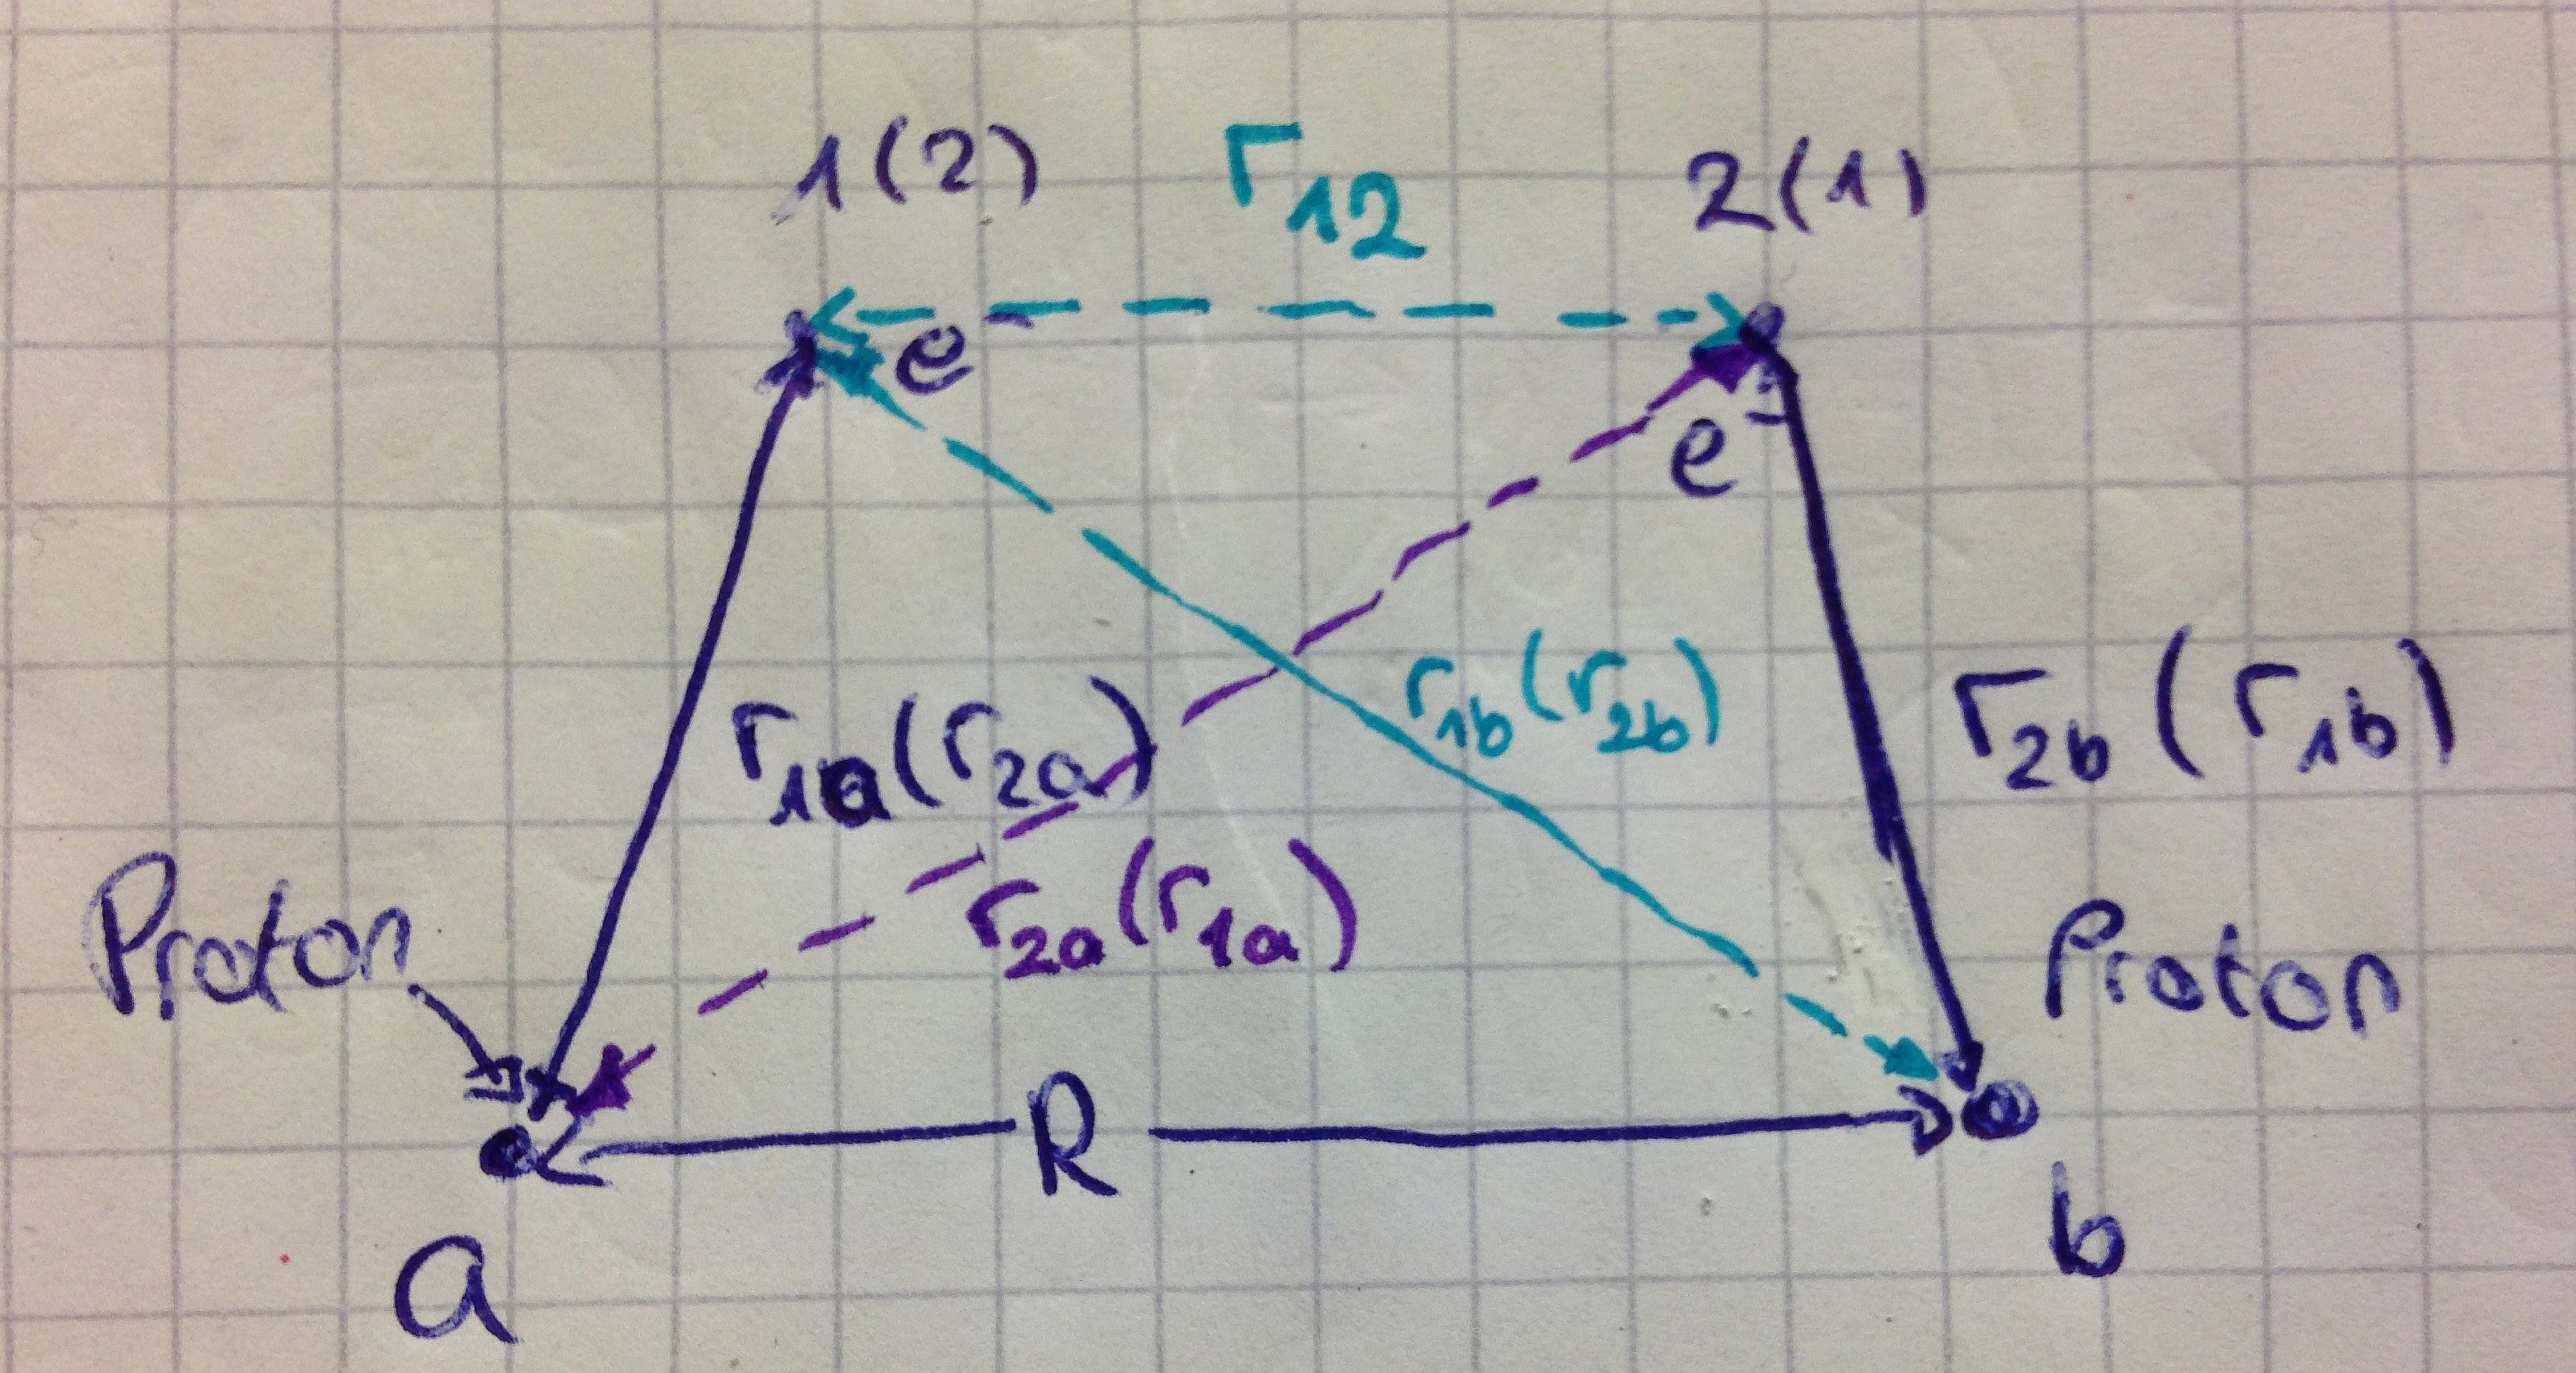
\includegraphics[width=10cm]{Homonukleare_Molekuele3}
		\end{center}
	\end{figure*}
	\begin{align*}
		\left(
		-\frac{\hbar^2}{2m_e} 
		\left(
		- \vec{\Delta}^2_1 - \vec{\Delta}^2_2
		\right) 
		V^{(R)}(\vec{r}_1, \vec{r}_2)
		\right)
		\Phi_n^{(R)} (\vec{r}_1, \vec{r}_2) 
		&= \U_n (R) \Phi_n^{(R)} (\vec{r}_1, \vec{r}_2) \\
		V^{(R)} (\vec{r}_1, \vec{r}_2) 
		&= \alpha \hbar c
		\left[
		\frac{1}{R} + \frac{1}{r_{12}} - \frac{1}{r_{1a}} - \frac{1}{r_{2b}} - \frac{1}{r_{1b}}
		- \frac{1}{r_{2a}}
		\right] \\
		(r_{12}, r_{1b} \text{ etc. Funktion von } R,\vec{r}_1, \vec{r}_2)
	\end{align*}
Betrachte Bahnwellenfunktion für große R:

Wasserstoffgrundzustand:
	\begin{align*}
		\psi (\vec{r}) &= \frac{1}{\sqrt{\pi a_{\mathrm{B}}^3}}
		e^{-\frac{r}{a_{\mathrm{B}}}} ,&
		E_1 &= -\frac{\alpha \hbar c}{2 a_{\mathrm{B}}} ,&
		a_{\mathrm{B}} &= \frac{\hbar}{m c \alpha} \text{ Bohr-Radius}
	\end{align*}
Ansatz für Wellenfunktion $\Phi(\vec{r}_1, \vec{r}_2)$
	\begin{align*}
		\Phi_1 (\vec{r}_1, \vec{r}_2) &= \psi (r_{1a}) \psi(r_{2b}) \\
		\Phi_2 (\vec{r}_1, \vec{r}_2) &= \psi (r_{1b}) \psi(r_{2a})
	\end{align*}
Heitler-London (1927) Ansatz:
	\begin{align*}
		\Phi^g &\propto \Phi_1 + \Phi_2 ,&
		\Phi^u &\propto \Phi_1 - \Phi_2
	\end{align*} 
Testwellenfunktion für Variationsverfahren
	\begin{align*}
		\ket{\Phi} &= \ket{\Phi_1} + \lambda \ket{\Phi_2}
		& \lambda \in \mathds{R} \text{ ist freier Parameter}
	\end{align*}
	\begin{align*}
		\U_0 \leq W(R) &=
		\frac{\braket{\Phi_1 + \lambda \Phi_2 | H | \Phi_1 + \lambda \Phi_2}}{\braket{\Phi_1 + \lambda \Phi_2 | \Phi_1 + \lambda \Phi_2}} \\
		&= \frac{\braket{\Phi_1 | H | \Phi_1} + \lambda^2 \braket{\Phi_2 | H | \Phi_2} + 2 \lambda \mathrm{Re} \left(\braket{\Phi_1 | H | \Phi_2}\right)}{1 + \lambda^2 + 2 \lambda \mathrm{Re} \braket{\Phi_1 | \Phi_2}} \\
		&= \frac{(1 + \lambda^2) H_{11} + 2 \lambda H_{12}}{1 + \lambda^2 + 2 \lambda S^2}
		(*)
	\end{align*} 
mit
	\begin{align*}
		H_{11} &= \braket{\Phi_1 | H | \Phi_1} = \braket{\Phi_2 | H | \Phi_2}\\
		H_{12} &= \mathrm{Re} \braket{\Phi_1 | H | \Phi_2}\\
		S^2 &= \mathrm{Re} \braket{\Phi_1 | \Phi_2} \rightarrow
		\left\{
		\begin{aligned}
			1 &,~ R \rightarrow 0 \\
			0 &,~ R \rightarrow \infty
		\end{aligned}
		\right.
	\end{align*}
Wie muss ich $\lambda$ wählen, damit $W(R)$ minimal ist?
	\begin{align*}
		\frac{\partial W}{\partial \lambda} 
		&= \frac{(2 \lambda H_{11} + 2 H_{12}) (1 + \lambda^2 + 2 \lambda S^2) - (2 \lambda + 2 S^2) ((\lambda^2 + 1)H_{11} + 2 \lambda H_{12})}{(\lambda^2 + 2 \lambda S^2 + 1)^2}
		= 0 \\
		\frac{\partial W}{\partial \lambda} &\propto \ldots 
		= (H_{12} - H_{11} S^2) (1 - \lambda^2)\\
		&\Rightarrow \lambda = + 1 \text{ oder } \lambda = -1
	\end{align*}
(Heitler - London Ansatz ergibt sich als Lösung des Variationsproblems)
	\begin{align*}
		\lambda &= \pm 1 \Rightarrow \U^{g \text{ oder }u} (R) 
		\overset{*}{\leq} \frac{H_{11} \pm H_{12}}{1 \pm S^2} \\
		S^2 &= \mathrm{Re}\braket{\Phi_1 | \Phi_2} 
		= \mathrm{Re} \int \diff^3 r_1 \diff^2 r_2 \psi^* (r_{1a}) \psi^* (r_{2b}) \psi(r_{1b}) \psi (r_{2a}) \\
		&= \mathrm{Re} \left(\int \diff^3 r_1 \psi^*(r_1a) \psi (r_{1b})\right)^2 \\
	\end{align*}
	\begin{align*}
		H_{11} &= \braket{\Phi_1 | H | \Phi_2} =
		\frac{\alpha \hbar c}{R} + 2 E_1 + K(R)
	\end{align*}
Wobei 
	\begin{align*}
		K(R) &= \alpha \hbar c \int \diff^3 r_1 \diff^3 r_2 |\psi (r_1a)|^2 
		|\psi (r_{2b})|^2 \left(\frac{1}{r_{12}} - \frac{1}{r_{2a}} - \frac{1}{r_{1b}}\right) \\
		&= \text{ Coulombpotential}
	\end{align*}
	\begin{align*}
		H_{12} = \mathrm{Re} (\braket{\Phi_1 | H | \Phi_2}) 
		= \left(\frac{\alpha \hbar c}{R} + 2 E_1\right) S^2 + A(R) 
	\end{align*}
mit 
	\begin{align*}
		A(R) &= \alpha \hbar c \mathrm{Re} \int \diff^3 r_1 \diff^3 r_2 \psi^* (r_{1a}) \psi^* (r_{2b}) \psi(r_{1b}) \psi (r_{2a}) \left(\frac{1}{r_{1a}} - \frac{1}{r_{2a}} - \frac{1}{r_{1b}}\right)\\
		&= \text{ Austauschintegral}
	\end{align*}
	\begin{align*}
		\U^{g \text{ oder }u} (R) &\leq 2 E_1 + \frac{\alpha \hbar c}{R} + 
		\frac{K(R) \pm A(R)}{1 \pm S^2(R)} \\
		R \text{ klein}:& \\
		S^2 &= 1 + \mathscr{O} (R^2) ,&
		K(R) &= - \frac{11}{8} \frac{\alpha \hbar c}{a_{\mathrm{B}}} + \mathscr{O} (R) \\
		& & &= A(R) + \mathscr{O} (R)\\
		&\overset{R \text{ klein}}{\Rightarrow} U^g - 2E_1 = \alpha \hbar c 
		\left(\frac{1}{R} - \frac{11}{8 a_{\mathrm{B}}}\right) 
	\end{align*}
	\begin{figure*} [h]
		\begin{center}
			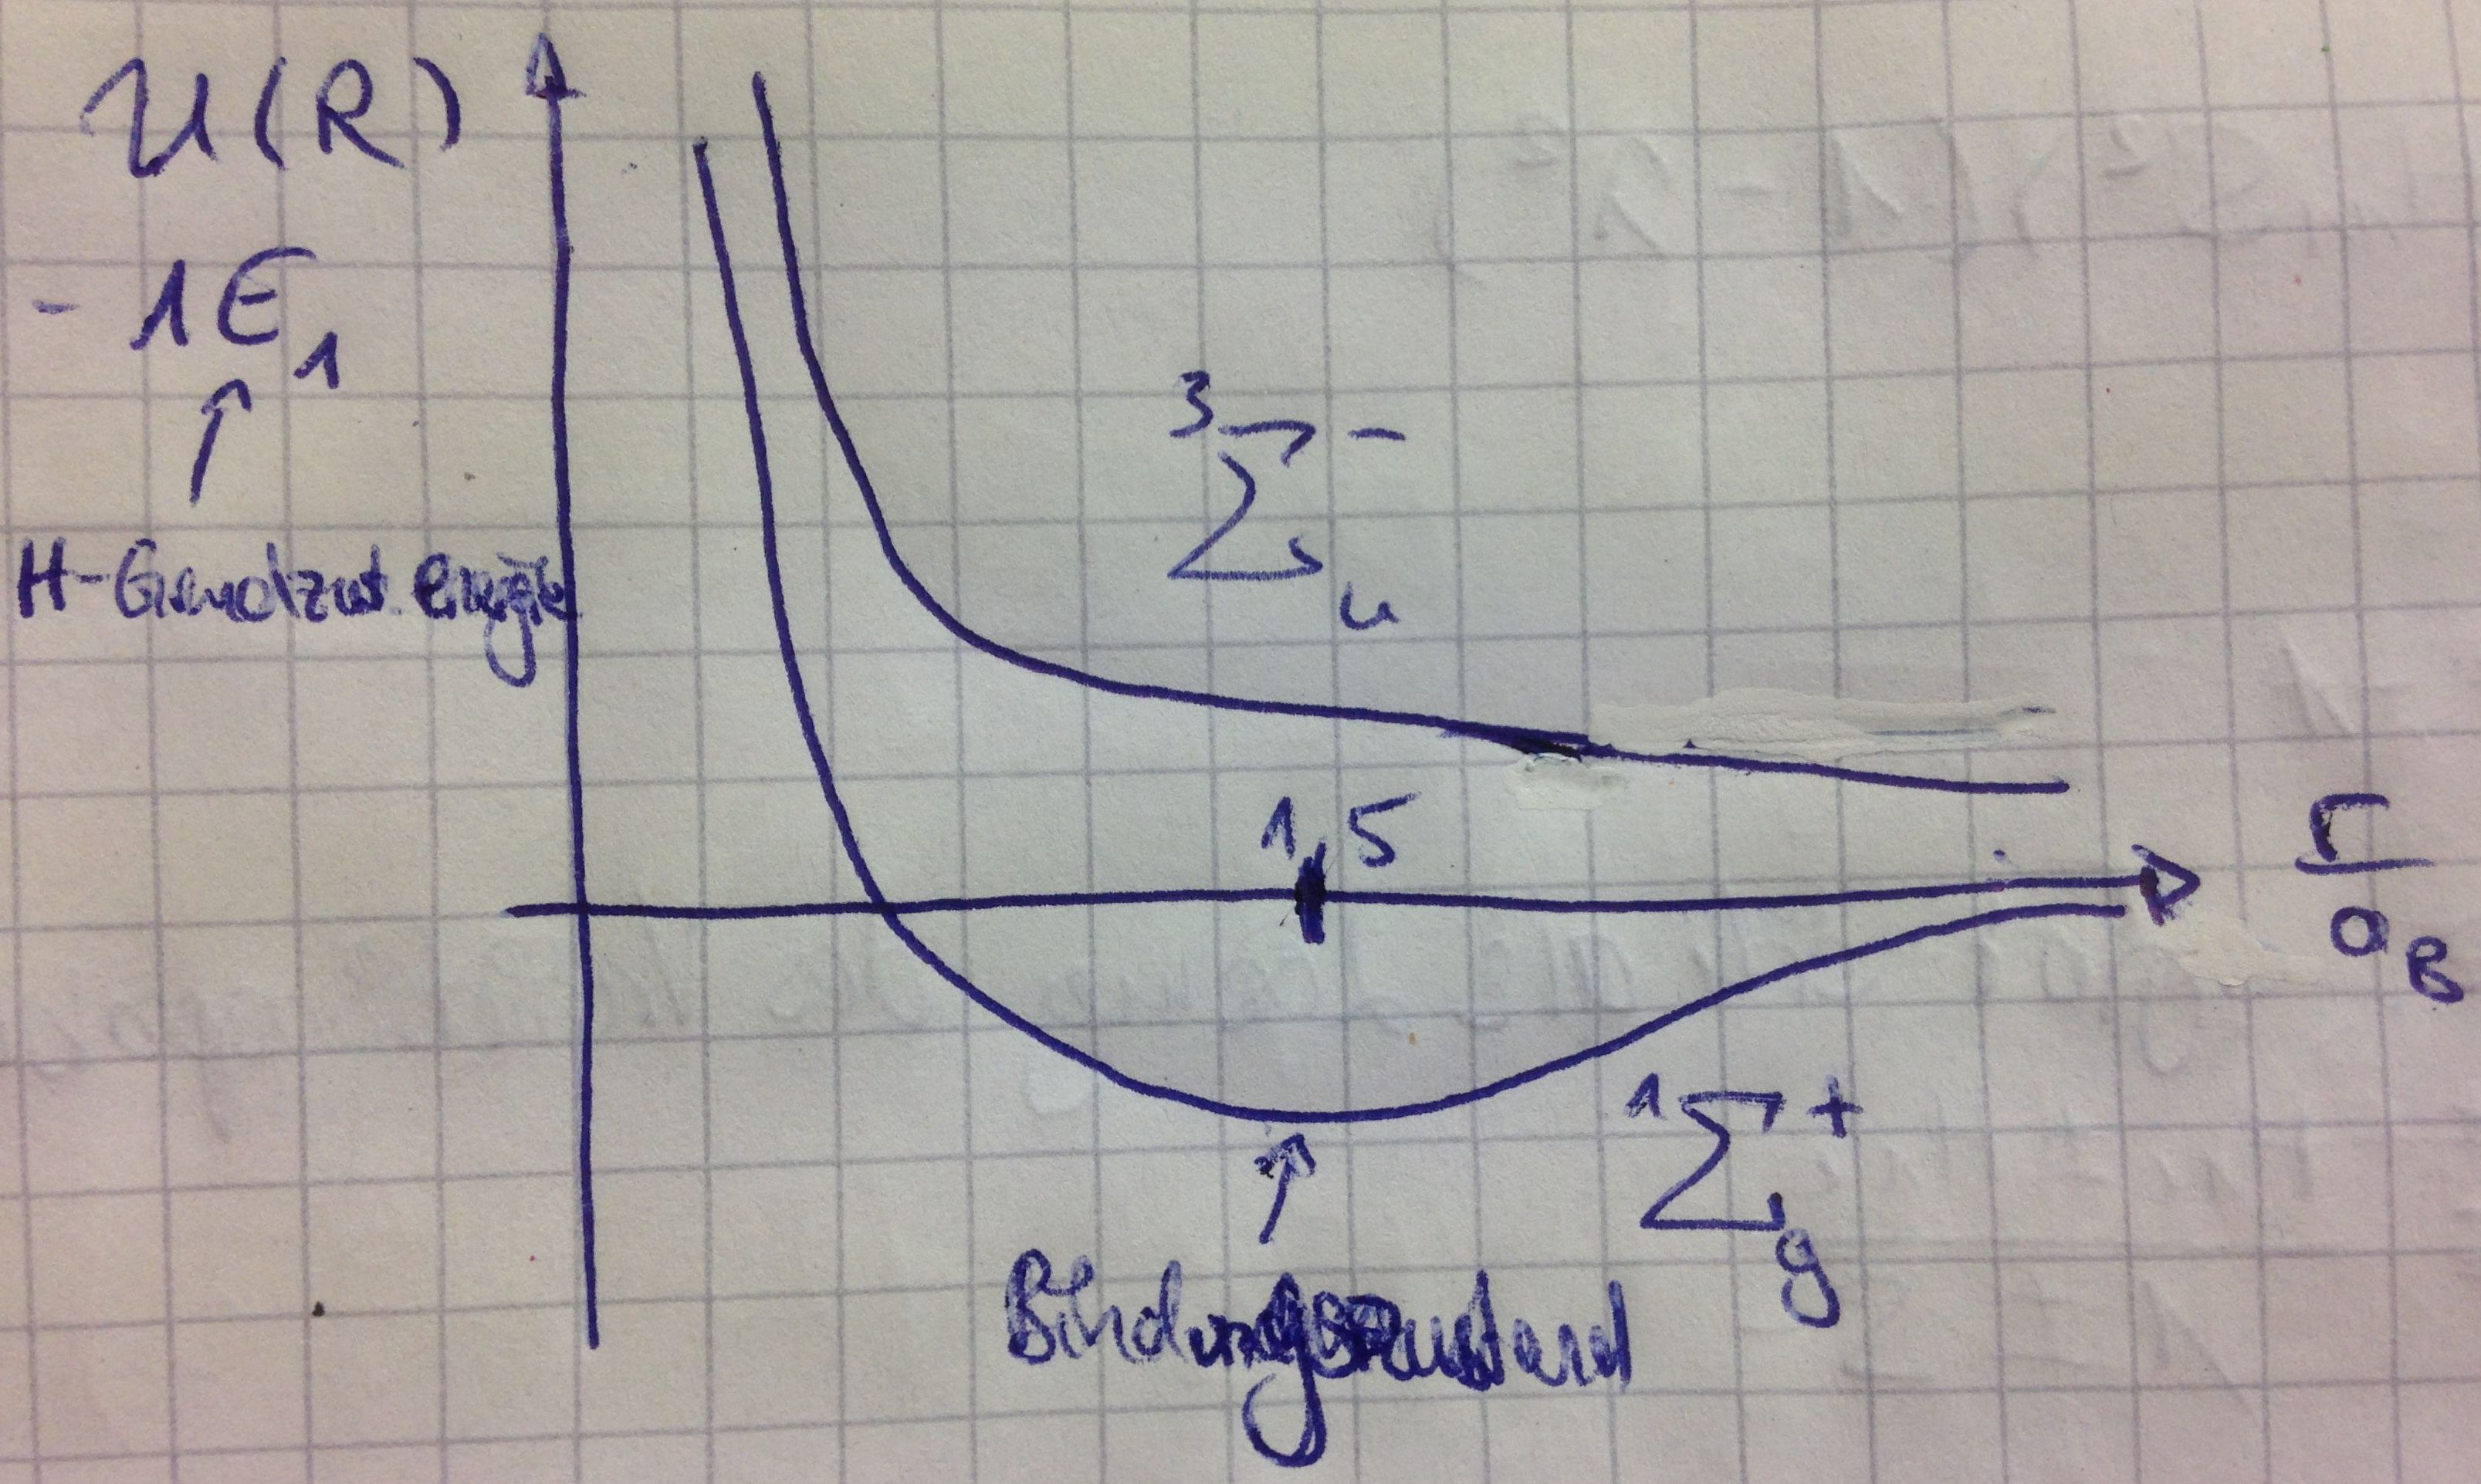
\includegraphics[width=10cm]{Homonukleare_Molekuele4}
		\end{center}
	\end{figure*}
\FloatBarrier
	\begin{tabular}{l | c | c | c}
		 & Heitler-London & Variation mit $Z \rightarrow Z^+ \mp 1$ & Natur \\
		 \hline 
		Bandlänge: $R_0$ & 0,08 nm & 0,076 nm & 0,074 nm \\
		Bindungsenergie: $\U (R_0) - 2E_1$ & $-3,14 e$V & $-3,76 e$V & $-4,48 e$V \\ 
	\end{tabular}

%	Kap 4
	\section{Relativistische Quantenmechanik}
	\subsection{Die Dirac-Gleichung}
NR QM:
	\begin{align*}
		H &= \frac{p^2}{2m} 
		& \vec{p} &\mapsto \hat{\vec{p}} = -i \hbar \vec{\nabla} \\
		& & E &\mapsto H = i \hbar \frac{\partial}{\partial t} \\
		i \hbar \frac{\partial}{\partial t} \ket{\psi} 
		&= \frac{\hat{p}^2}{2m} \ket{\psi} 
	\end{align*}
Spezielle Relativitätstheorie:
	\begin{align*}
		H^2 &= p^2 c^2 + m^2 c^4 
		&\Rightarrow H &= \sqrt{p^2c^2 +m^2 c^4} 
		= mc^2\left(1 + \frac{\vec{p}^2}{2m} - \frac{(\vec{p}^2)^2}{8 m^4 c^4} + \ldots\right)
	\end{align*}
Relativistische Schrödinger Gleichung (?):
	\begin{align*}
		i \hbar \frac{\partial}{\partial t} \ket{\psi} 
		= \sqrt{p^2c^2 +m^2 c^4} \ket{\psi}
	\end{align*}
Ortsraum:
	\begin{align*}
		i \hbar \frac{\partial}{\partial t} \ket{\psi} 
		= mc^2 \left(1 - \frac{\vec{\hbar^2}}{2mc^2}\vec{\nabla}^2 - \frac{\hbar^2(\vec{\nabla}^2)^2}{8 m^4 c^4}\right)
	\end{align*}
	\begin{enumerate}
		\item unsymmetrisch im Raum und Zeit (nicht forminvariant unter Lorentz-Transformation)
		\item Hohe Ableitungen
	\end{enumerate}
Zwei Möglichkeiten der relativen Verallgemeinerung der (freien) Schrödingergleichung 
\marginpar{?? punkt 2 kam nie vor}
	\begin{align*}
		H^2 \ket{\psi} &= (c^2 \hat{p}^2 + m^2 c^4) \ket{\psi} \\
		-\hbar^2 \frac{\partial^2 \psi}{\partial t^2}
		&= (-\hbar^2 c^2 \vec{\nabla}^2 + m^2 c^4) \psi (\vec{r} , t) \\
		&\Rightarrow
		\boxed{
			\left(
			\frac{1}{c^2} \frac{\partial^2 \psi}{\partial t^2} - \vec{\nabla}^2 
			+ \left(\frac{mc}{\hbar}\right)^2
			\right)
			\psi (\vec{r} , t) = 0
		}
	\end{align*} 
Klein-Gordon-Gleichung, und $\frac{1}{c^2} \frac{\partial^2 \psi}{\partial t^2} - \vec{\nabla}^2 = \Box$ d'Alembertoperator.

Kein ``Spin'' Möglich für skalare Teilchen

Spin $=0$: Higgs, Pionen, $\alpha-$Teilchen etc.
\\
Dirac: erste Ableitun in $t \Rightarrow$ sollte linear in $p_x, p_y, p_z$ sein, damit forminvariant unter Lorentz-Transformation.

Ansatz:
	\begin{align*}
		H^2 &= p^2 c^2 + m^2 c^4 = c^2 (\vec{\alpha} \cdot \vec{p} + \beta m c)^2\\
		&= c^2 
		\left[
			\alpha_x^2 p_x^2 + \alpha_y^2 p_y^2 +\alpha_z^2 p_z^2
			+ \beta^2m^2c^2 + \alpha_x \beta p_x m c + \beta \alpha_x p_x mc \right.\\
			&\left.\vphantom{\alpha_x^2 p_x^2} + \{\alpha_y, \beta\} p_y mc + \{\alpha_z \beta \} p_z mc 
			+ \{\alpha_x, \alpha_y\} p_x p_y + \{\alpha_y, \alpha_z\} p_y p_z
			+\{\alpha_z, \alpha_x\}p_z p_x
 		\right]
	\end{align*}
Koeffizientenvergleich:
	\begin{align*}
		\alpha_x^2 &= \alpha_y^2 = \alpha_z^2 = 1 = \beta^2
		& &\boxed{\{\alpha_i, \beta \} = 0}\\
		& & &\{\alpha_i, \beta \} = 0 \text{ für } i \neq j \\
		&\Rightarrow \boxed{\{\alpha_i, \beta \} = 2 \delta_{ij}}
	\end{align*}
$\Rightarrow \alpha_i, \beta$ sind keine Zahlen. (vllt Matrizen?)
	\begin{align*}
		\alpha_i &= \alpha_i^\dagger ,&
		\beta &= \beta^\dagger ,& 
		\text{weil } H &= H^\dagger \\
		\text{EW }: \alpha_i^2 &= \mathds{1} ,&
		\beta^2 &= \mathds{1} 
		&\Rightarrow \mathrm{ EW } &\in \{\pm 1\}  
	\end{align*}
	\begin{align*}
		\mathrm{Sp}(\alpha_x) = \mathrm{Sp}(\alpha_x\alpha_y^2) 
		= \mathrm{Sp} (\alpha_y \alpha_x \alpha_y) 
		= - \mathrm{Sp}(\alpha_x \alpha_y^2) = -\mathrm{Sp}(\alpha_x) = 0
	\end{align*}
$\alpha_i, \beta$ sind spurlose hermitesche Matrizen mit EW $\pm 1$
	\begin{align*}
		\text{spurlos } \Rightarrow \# (\mathrm{EW } = + 1)
		= \# (\mathrm{EW } = - 1) \Rightarrow \text{ Dimension }d\text{ gerade}
	\end{align*}
Bei $d=2$ haben wir die Paulimatrizen: Basis über $\mathds{R}$ aller spurlosen hermiteschen $2 \times 2$ Matrizen.
	\begin{align*}
		\sigma_x &=
		\begin{pmatrix}
		0 & 1 \\
		1 & 0
		\end{pmatrix}&
		\sigma_y &=
		\begin{pmatrix}
		0 & -i \\
		i & 0
		\end{pmatrix}&
		\sigma_z &= 
		\begin{pmatrix}
		1 & 0 \\
		0 & -1
		\end{pmatrix} \\
		\{\sigma_i, \sigma_j\} &= 2 \delta_{ij} 
		&\text{Nehme } \sigma_0 &=
		\begin{pmatrix}
		1 & 0 \\
		0 & 1
		\end{pmatrix}
		= \mathds{1}_2 \text{ hinzu} 
	\end{align*}
Problem: $\mathds{1}_2$ ist nicht spurlos

Kleinste mögliche Dimension ist $d = 4$
\\
Dirac- $\alpha,\beta$ Matrizen:
	\begin{align*}
		\vec{\alpha} &=
		\begin{pmatrix}
		0 & \vec{\sigma} \\
		\vec{\sigma} & 0
		\end{pmatrix} 
		& 4 \times 4 \text{ Matrix Beispiel: }
		\alpha_z &=
		\begin{pmatrix}
		0 & \sigma_z \\
		\sigma_z & 0
		\end{pmatrix}
		=
		\begin{pmatrix}
		0 & 0 & 1 & 0 \\
		0 & 0 & 0 & -1 \\
		1 & 0 & 0 & 0\\
		0 & -1 & 0 & 0
		\end{pmatrix} \\
		\beta &=
		\begin{pmatrix}
		\mathds{1}_2 & 0 \\
		0 & \mathds{1}_2
		\end{pmatrix}
	\end{align*}
$\vec{\alpha}, \beta$ sind nicht eindeutig festgelegt, da auch $\vec{\alpha}', \beta'$ mit 
$\alpha_i' = \U^\dagger \alpha_i \U,~ \beta' = \U^\dagger \beta \U$ ($\U$ unitäre Matrix) obige Bedingungen erfüllen.
	\begin{align*}
		-i\hbar \frac{\partial}{\partial t} \ket{\psi}
		&= \left(\vec{\alpha} c \vec{p} + \beta m c^2\right) \ket{\psi} \\
		\text{Ortsraum } i\hbar \frac{\partial \psi (\vec{r}, t)}{\partial t}
		&= \left(-i\hbar c \vec{\alpha} \vec{\nabla} + \beta m c^2\right) \psi (\vec{r}, t)
	\end{align*}
DGL 1.Ordnung in $\frac{\partial}{\partial t}$ und $\frac{\partial}{\partial x}, \frac{\partial}{\partial y}, \frac{\partial}{\partial z}$ aber $\psi (\vec{r}, t)$ hat 4 Komponenten.

$\Rightarrow$ Lorentz-Spinor
\\
 \marginpar{30.11.2015}
% Wdh
%	\begin{align*}
%		i \hbar \frac{\partial}{\partial t} \ket{\psi} &=
%		\left(c \vec{\alpha} \cdot \vec{p} + \beta m c^2\right) \ket{\psi}
%	\end{align*}
Dirac-Spinor (auch Lorentz-Spinor)
	\begin{align*}
		\psi (\vec{r}, t) &=
		\begin{pmatrix}
		\psi_1 (\vec{r}, t) \\
		\psi_2 (\vec{r}, t) \\
		\psi_3 (\vec{r}, t) \\
		\psi_4 (\vec{r}, t)
		\end{pmatrix} &
		\braket{\psi | \psi}
		&= \int \diff^3 r 
		\overbrace{\psi^\dagger (\vec{r}, t) \psi (\vec{r}, t)}^{\mathclap{\rho (\vec{r}, t)}} 
		= const.
	\end{align*}
Denn $H$ ist selbstadjungiert. 

$\leadsto$ Wahrscheinlichkeitsinterpretation mit $\braket{\psi | \psi} = 1$ ist möglich.
\\
Definiere Wahrscheinlichkeitsdichte $\rho (\vec{r}, t) = \psi^\dagger (\vec{r}, t) \psi (\vec{r}, t)$
	\begin{align*}
		\frac{\partial \rho}{\partial t} &= 
		\frac{\partial \psi^\dagger}{\partial t} \cdot \psi + \psi^\dagger \frac{\partial \psi}{\partial t} 
		= \left(
			\frac{\beta m c^2}{i \hbar} - \frac{\beta m c^2}{i \hbar} 
		\right)
		\psi^\dagger \psi - c\psi^\dagger \vec{\alpha} \vec{\nabla} \psi 
		- c \vec{\nabla} (\psi^\dagger \vec{\alpha}) \psi \\
		&= -c \vec{\nabla} (\psi^\dagger \vec{\alpha} \psi) 
	\end{align*}
	\begin{empheq}[box = \boxed]{align*}
		\Rightarrow \frac{\partial \rho}{\partial t} + \vec{\nabla} \vec{j} = 0&
		& &\text{mit } \vec{j} = c \psi^\dagger \alpha \psi \\
		\text{ Kontinuiätsgleichung}& & &\text{Wahrscheinlichkeitsstromdichte}
	\end{empheq}
	\begin{align*}
		4 \text{ Vektoren } (X^\mu) &= (X^0, \vec{X})
		& (X_\mu) &= (\eta_{\mu\nu} X^\nu) = (X^0, -\vec{X}) \\
		\eta_{\mu\nu} &=
		\begin{pmatrix}
			1 & 0 & 0 & 0 \\
			0 & -1 & 0 & 0 \\
			0 & 0 & -1 & 0 \\
			0 & 0 & 0 &-1
		\end{pmatrix} &
		\vec{X} &= 
		\begin{pmatrix}
		X^1 \\
		X^2 \\
		X^3 \\
		X^4 
		\end{pmatrix} \\
		\frac{\partial}{\partial X^\mu} X^\nu 
		&= \partial_\mu^\nu 
		\leadsto \partial_\mu = \frac{\partial}{\partial X^\mu}
	\end{align*}
(aus unten oben wird oben unten) $\partial_\mu X^\nu = \partial_\mu^\nu$
	\begin{align*}
		\left(\partial_\mu\right) 
		&= \left(\frac{\partial}{\partial X^\mu}\right)
		= (\partial_0, \vec{\nabla}) &
		(\partial^\mu) &=
		\left(\frac{\partial}{\partial X_\mu}\right)
		= (\partial^0, -\vec{\nabla}) \\
		\partial_0 &= \frac{\partial}{\partial X^0} = \frac{1}{c} \frac{\partial}{\partial t}
		& X^0 &= ct \\
		\vec{p} &= -i\hbar \vec{\nabla} ,&
		E &= i \hbar \frac{\partial}{\partial t} = i \hbar c \frac{\partial}{\partial X^0} 
	\end{align*}
4-Impuls $(p^\mu) = (E/c, \vec{p})$
	\begin{align*}
		p_\mu p^\mu &= \frac{E^2}{c^2} - \vec{p}^2 = m^2 c^2,&
		\text{denn } E^2 &= m^2 c^4 + \vec{p}^2 c^2 \\
		(p_\mu) &= \left(\frac{E}{c}, -\vec{p}\right) = i\hbar (\partial_0, \vec{\nabla})
	\end{align*}
	\begin{align*}
		0 &= \left(
			-i \hbar c \vec{\alpha}_i \vec{\nabla} - i\hbar \frac{\partial}{\partial t}
			+ \beta m c^2
		\right) \psi(\vec{r}, t) & 
		&\left.\vphantom{\left(\frac{\partial}{\partial t}\right)}\right| \cdot (-\beta) \\
		0 &= \left[
			i \hbar \left(\beta \frac{\partial}{\partial X^0} \beta \vec{\alpha} \vec{\nabla}\right)
			- mc
		\right] \psi (\vec{r}, t) \\
		\gamma^0 &= \beta ~,~~ \gamma^i =\beta \alpha^i \\
		0 &= \left(i \hbar 
			\left(\gamma^0 \frac{\partial}{\partial X^0} + \vec{\gamma} \cdot \vec{\nabla}\right)
			- mc
		\right) \psi (\vec{r}, t) 
	\end{align*}
	\begin{empheq}[box = \boxed]{align*}
		(i\hbar \gamma^\mu \partial_\mu - mc) \psi(\vec{r}, t) &= 0 \\
		\text{oder } (\gamma^\mu p_\mu - mc) \ket{\psi} &= 0
	\end{empheq}
Dirac Gleichung
	
Offensichtlich ist dies forminvariant unter Lorentz-Transformationen (relativistisch kovariant)
	\begin{align*}
		\gamma^0 &= \beta =
		\begin{pmatrix}
			\mathds{1} & 0 \\
			0 & -\mathds{1}
		\end{pmatrix}
		& \beta \cdot \alpha^i &= -\alpha^i \beta &
		&\{\alpha^i, \beta \} = 0 \\
		\vec{\gamma} &= \beta \vec{\alpha} =
		\begin{pmatrix}
			0 & \vec{\sigma} \\
			\vec{\sigma} & 0
		\end{pmatrix} &
		(\gamma^i)^\dagger &= (\beta \alpha^i)^\dagger
		= (\alpha^i)^\dagger \beta^\dagger \\
		& & &= \alpha^i \beta = -\beta \alpha^i = -\gamma^i
		& &\text{ (anti-hermitesch)} \\
		\gamma^0 &= (\gamma^0)^\dagger 
		& \boxed{(\gamma^\mu)^\dagger = \gamma^0 \gamma^\mu \gamma^0}&
	\end{align*}
	\begin{align*}
		\{\gamma^\mu, \gamma^\nu\} &= 2 g^{\mu \nu} = \mathds{1}_4\\
		\{\gamma^i, \gamma^j\} &=
		\{\beta \alpha^i, \beta \alpha^j\}
		= - \beta^2 \{\alpha^i, \alpha^j\} = -2 \delta^{ij} \mathds{1}\\
		\left[
			(\gamma^\mu p_\mu - m c) \psi
		\right]^\dagger &= 0 
		= \psi^\dagger (\gamma^{\mu \dagger} p_\mu - mc) \\
		&= \psi^\dagger \left(
			\gamma^0 \gamma^\mu p_\mu \gamma^0 - \gamma^0 mc \gamma^0
		\right) \\
		0 &= \psi^\dagger \gamma^0 (\gamma^\mu p_\mu - mc) \\
		\overline{\psi} \coloneqq \psi^\dagger \gamma^0
	\end{align*}
Wahrscheinlichkeitsstromdichte (0-Komponente):
	\begin{align*}
		j^0 &= c \rho = c \psi^\dagger \psi = c \overline{\psi} \gamma^0 \psi \\
		\frac{\partial \rho}{\partial t}
		&= \partial_0 j^0 = -\vec{\nabla} \psi^\dagger \vec{\alpha} \psi 
		= - \partial_i \overline{\psi}
		\underbrace{\gamma^0 \alpha^i}_{\mathclap{\beta \alpha^i = \gamma^i}} \psi \\
		\Rightarrow \partial_\mu 
		\underbrace{\overline{\psi} \gamma^\mu \psi}_{\mathclap{\text{Der 4-Strom }j^\mu \text{ ist erhalten}}} &= 0 ~~\text{(Kontinuitätsgleichung)}
	\end{align*}
	\begin{align*}
		\psi &=
		\begin{pmatrix}
			\psi_1 \\
			\psi_2 \\
			\psi_3 \\
			\psi_4
		\end{pmatrix}
		&\Rightarrow \overline{\psi} &=
		(\psi_1^*, \psi_2^*, -\psi_3^*, -\psi_4^*) 
	\end{align*}
Ansatz ebene Welle:
	\begin{align*}
		\psi (\vec{r}, t) &=
		u(\vec{k}) e^{i(\vec{k}\vec{r} - \omega(\vec{k}) t)} \\
		&= u(\vec{k}) e^{ik.x} 
		& k. x &= k_\mu X^\mu \\
		\vec{X} &= \vec{r} ,& X^0 &= ct,& k^0 &= \frac{\omega}{c} \\
		u &=
		\begin{pmatrix}
			u_1 \\
			u_2 \\
			u_3 \\
			u_4
		\end{pmatrix}
		~ \text{ Dirac Spinor}
	\end{align*}
	\begin{align*}
		\left(i \hbar \gamma^\mu \partial_\mu - mc\right)
		\psi(\vec{r}, t) &= 0 \\
		\text{ist OK für } p_\mu p^\mu &= m^2 c^2 \\
		\Rightarrow (\gamma^\mu p_\mu - mc) u \left(\vec{k} = \frac{\vec{p}}{\hbar}\right) &= 0 
	\end{align*}
Lösung für $\vec{p} = \vec{0}$ mit 
$ \gamma^0= \begin{pmatrix}
1 & & \\
& 1 && \\
&& -1 & \\
&&& -1 
\end{pmatrix}$
	\begin{align*}
		(\gamma^0 p_0 - mc) u = 0 \Rightarrow
		(E-mc^2) u_1 &= 0 \\
		(E-mc^2) u_2 &= 0 \\
		(-E-mc^2) u_3 &= 0 \\
		(-E-mc^2) u_4 &= 0 \\
	\end{align*}
	\begin{align*}
		\Rightarrow 4 \text{ Lösungen }: 
		E &= mc^2 ,& u^{(1)} &= (1, 0 ,0 ,0)^t &\text{ oder } 
		u^{(2)} &= (0,1,0,0)^t \\
		E &= -mc^2 ,& u^{(3)} &= (0, 0, 1, 0)^t &\text{ oder }
		u^{(4)} &= (0,0,0,1)^t
	\end{align*}
Beliebiger Impuls:
	\begin{align*}
	u &= 
		\begin{pmatrix}
			\phi \\
			\chi
		\end{pmatrix} &
	\phi &= 
		\begin{pmatrix}
		\phi_1 \\
		\phi_2
		\end{pmatrix} &
	\chi &= 
		\begin{pmatrix}
		\chi_1 \\
		\chi_2
		\end{pmatrix}
	\end{align*}
	\begin{align*}
		\left( \gamma^\mu p_\mu - mc\right) u
		&=\left[
			\gamma^0 \left(
				\mathds{1} p_0 +
					\begin{pmatrix}
						0 & \vec{\sigma} \\
						\vec{\sigma} & 0
					\end{pmatrix} \vec{p}
				\right)
			-mc \mathds{1}
		\right]
		\begin{pmatrix}
			\phi \\
			\chi
		\end{pmatrix} \\
		&= \begin{pmatrix}
			(p_0 -mc) \phi - (\vec{p} ~\vec{\sigma}) \chi \\
			(-p_0 -mc) \chi - (\vec{p} ~\vec{\sigma}) \phi
		\end{pmatrix}
		= \vec{0}
	\end{align*}
	\begin{align*}
		\text{2.Zeile: }
		\chi &= \frac{- \vec{p}~\vec{\sigma}}{p_0 +mc} \phi 
		& (\vec{A}\vec{\sigma})(\vec{B}\vec{\sigma}) &=
		\vec{A}\vec{B}+ i \vec{\sigma} (\vec{A} \times \vec{B}) \\
		\text{1.Zeile: } 
		\phi &= - \frac{\vec{p}~\vec{\sigma}}{p_0 - mc} \chi \\
		&= \frac{(\vec{p}~\vec{\sigma})(\vec{p}~\vec{\sigma})}{p_0^2-m^2c^2} \phi \\
		&= \frac{\vec{p}^2}{\vec{p}^2}\phi = \phi \checkmark
	\end{align*}
Also $\phi$ und $\chi$ nicht linear unabhängig.
	\begin{align*}
		\boxed{E^2 = \vec{p}^2c^2 + m^2 c^4}
	\end{align*}
$\Rightarrow$ Es existieren ebene Wellen als Lösungen der Dirac Gleichung, wobei $\phi$ oder $\chi$ frei gewählt werden kann.

2 Fälle (analog zum $\vec{p}= \vec{0}$ Fall)
	\begin{enumerate}[1.]
		\item $E= \sqrt{m^2c^4 + \vec{p}^2 c^2}$
		\begin{align*}
			\psi (x) &= u(\vec{k}) e^{-ik.x} \\
			\phi^{(1)} &= 
			\begin{pmatrix}
			1 \\ 0
			\end{pmatrix}
			&\Rightarrow 
			\chi^{(1)} &= \frac{\vec{p}~\vec{\sigma}}{p_0 + mc}
			\begin{pmatrix}
			1 \\ 0
			\end{pmatrix}
			= \frac{c}{E + mc^2}
			\begin{pmatrix}
			p_3 \\ p_1 + ip_2
			\end{pmatrix} 
			\\
			\phi^{(2)} &= 
			\begin{pmatrix}
			0 \\ 1
			\end{pmatrix}
			&\Rightarrow 
			\chi^{(2)} &= \frac{\vec{p}~\vec{\sigma}}{p_0 + mc}
			\begin{pmatrix}
			0 \\ 1
			\end{pmatrix}
			= \frac{c}{E + mc^2}
			\begin{pmatrix}
			p_1 - ip_2 \\ -p_3
			\end{pmatrix}
		\end{align*}
	Nicht relativistischer Grenzfall:
		\begin{align*}
			E &= mc^2 + E' &\text{mit } E' &\ll mc^2 \\
			E' &\approx \frac{\vec{p}^2}{2m} &
			\left|\chi^{(i)} \right| &\ll \left|\phi^{(i)} \right| \\
			\phi &: \text{``große Komponenten''} ,& \chi &: \text{``kleine Komponenten''}
		\end{align*}
	\item $E=-\sqrt{m^2c^4 + \vec{p}^2 c^2}$
		\begin{align*}
			\psi &= u(\vec{k}) e^{-ik.x} \\
			\Rightarrow 
			\chi^{(3)} &= 
			\begin{pmatrix}
			1 \\ 0
			\end{pmatrix}
			&\Rightarrow 
			\phi^{(3)} &= \frac{\vec{p}~\vec{\sigma}}{-p_0 + mc}
			\begin{pmatrix}
			1 \\ 0
			\end{pmatrix}
			= \frac{c}{|E| + mc^2}
			\begin{pmatrix}
			p_3 \\ p_1 + ip_2
			\end{pmatrix} 
			\\
			\chi^{(4)} &= 
			\begin{pmatrix}
			0 \\ 1
			\end{pmatrix}
			&\Rightarrow 
			\phi^{(4)} &= \frac{\vec{p}~\vec{\sigma}}{-p_0 + mc}
			\begin{pmatrix}
			0 \\ 1
			\end{pmatrix}
			= \frac{c}{|E| + mc^2}
			\begin{pmatrix}
			p_1 - ip_2 \\ -p_3
			\end{pmatrix}
			\\
			\phi &: \text{``kleine Komponenten''} ,& \chi &: \text{``große Komponenten''}
		\end{align*}
	im nicht relativistischen Grenzfall.
	\end{enumerate}
Wdh.: Lösung \marginpar{03.12.2015}
der ``freien'' Dirac-Gleichung 
	\begin{align*}
		\psi &= u(\vec{k}) e^{-ik.x} ,&
		k^2 &= k_\mu k^\mu = \frac{m^2 c^2}{\hbar^2} \\
		u &=
		\begin{pmatrix}
		\phi \\
		\chi
		\end{pmatrix}
		\text{und } \phi, \chi \text{ sind Pauli-Spinoren}		
	\end{align*}
Lösung mit $E > 0 \leadsto \phi$ große Kompontenten 
\\
Lösung mit $E < 0 \leadsto \chi$ große Kompontenten

Interpretation:
	\begin{align*}
		E>0 &: \text{ Elektron} \\
		E<0 &: \text{ Positron mit } E>0 \text{ (Antiteilchen)}
	\end{align*}
Es zeigt sich, dass $m(\text{Elektron}) = m{(Positron)}$, 
\\aber Ladung $q(\text{Elektron}) = -q(\text{Positron}) = -e$
\newpage
Dirac: ``Dirac''-See
	\begin{figure*} [h]
		\begin{center}
			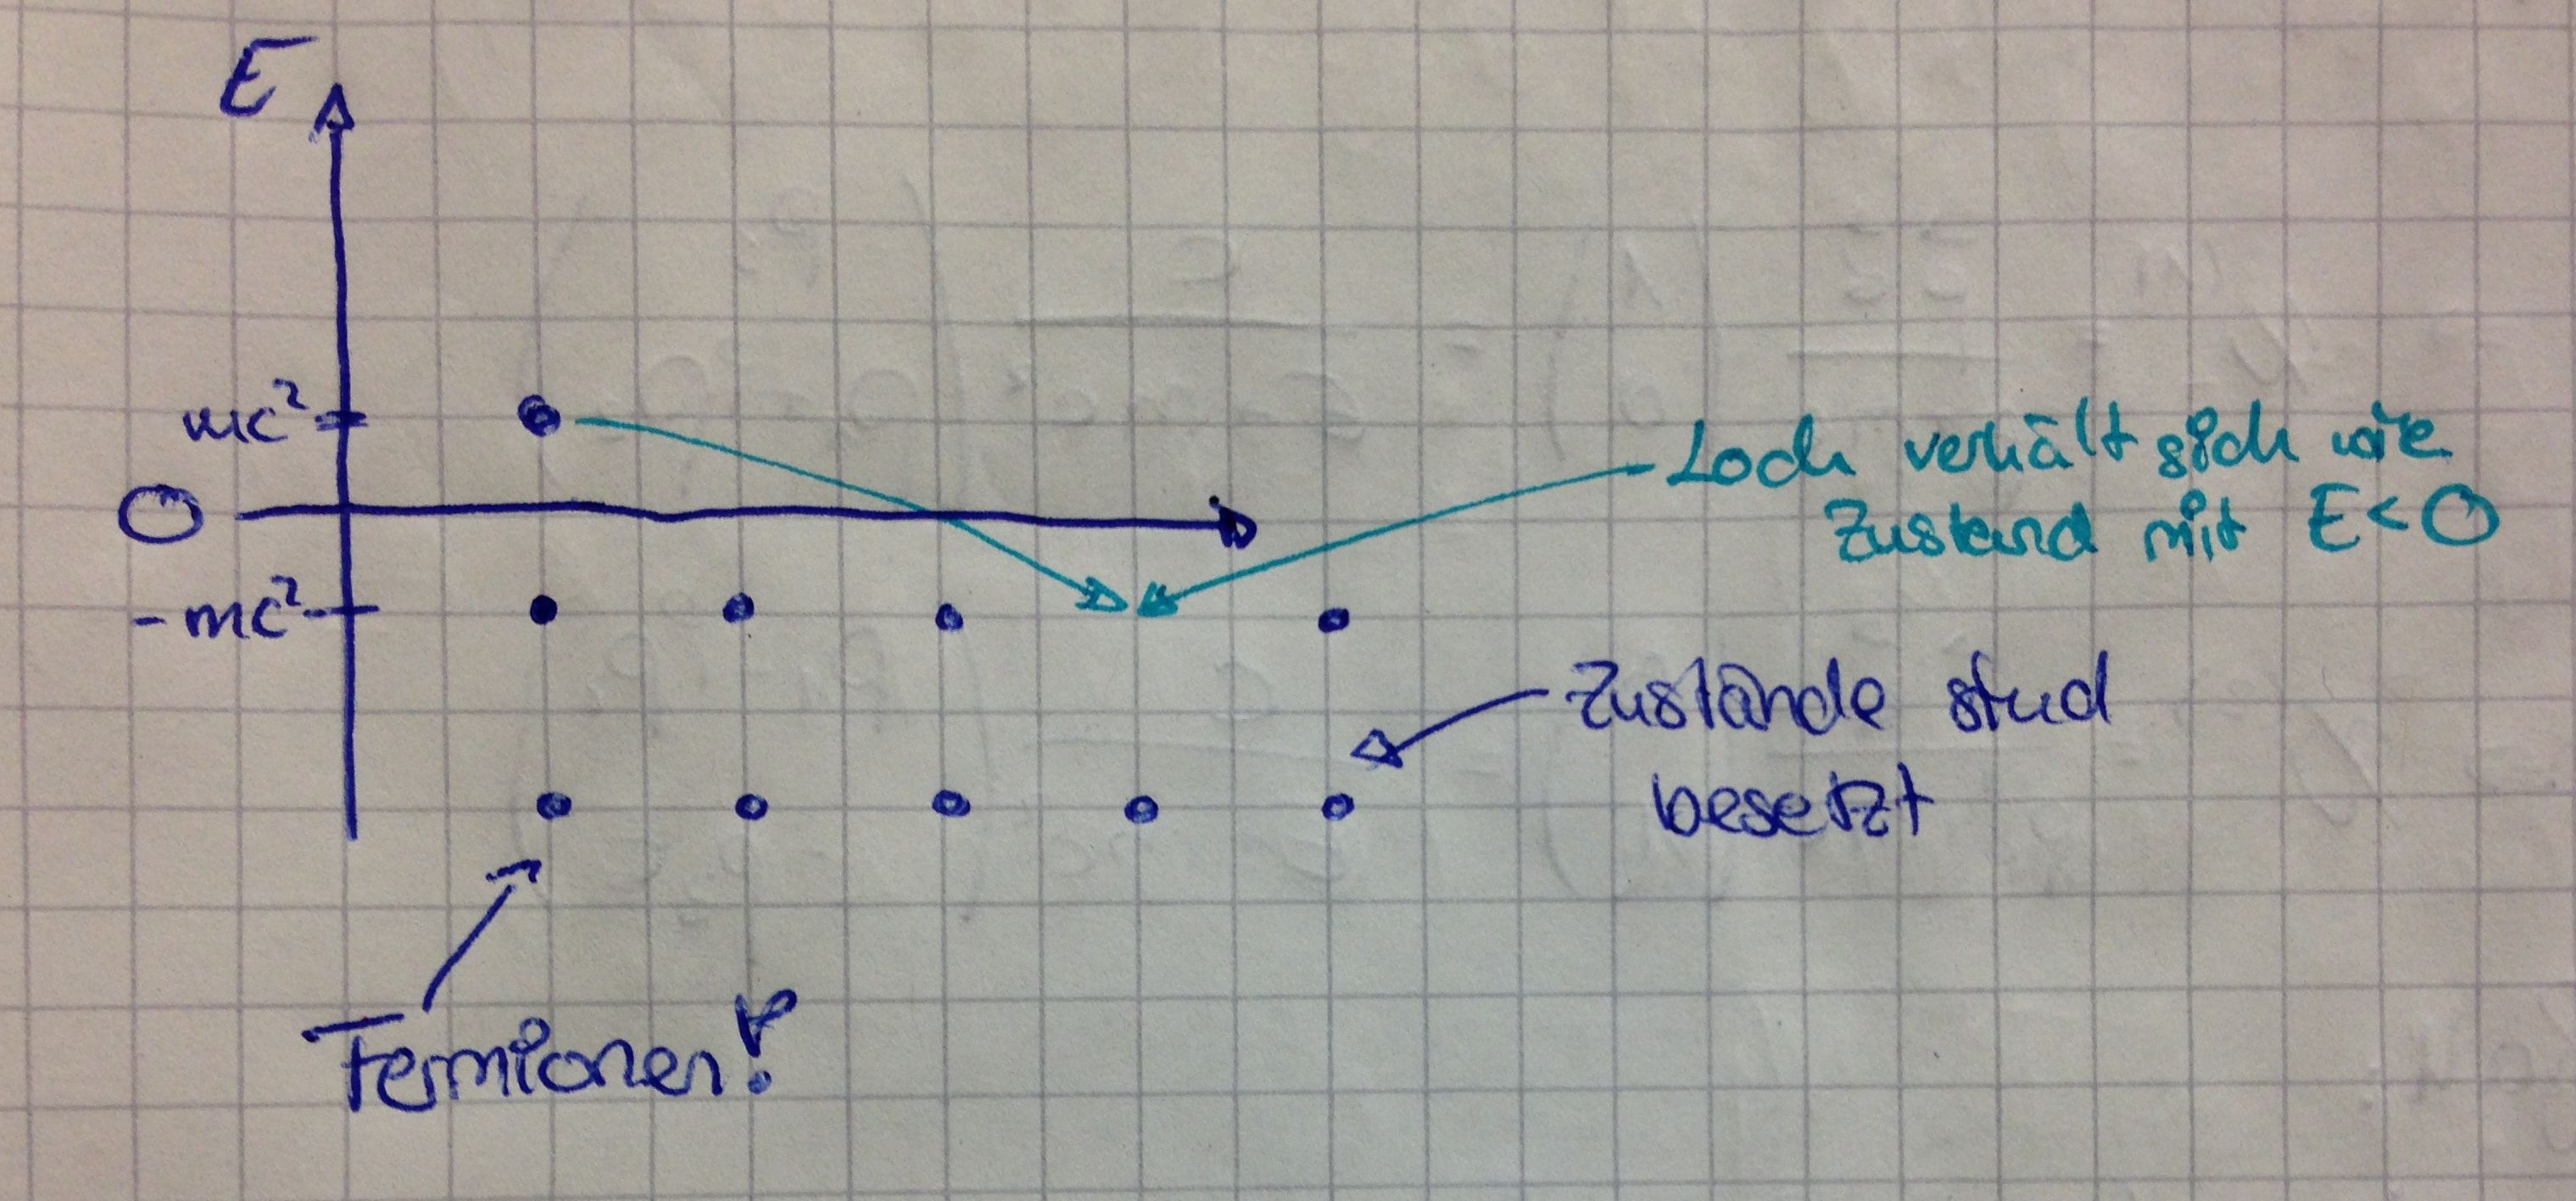
\includegraphics[width=10cm]{Dirac-Gleichung1}
		\end{center}
	\end{figure*}
	
	\\
	\begin{tabular}{l l}
		1928/9 & Vorhersage von Teilchen mit gleicher Masse, aber entgegengesetzter \\
		& Ladung des Elektrons (Dirac/Weyl) \\
		1932 & Entdeckung des Positrons (Anderson)
	\end{tabular}
	\subsection{Kopplung der Dirac-Gleichung an elektromagnetische Felder}
``Rezept'' aus QM1 (2)
	\begin{align*}
		\vec{p} &\mapsto \vec{p} - \frac{q}{c} \vec{A},&
		q &= -e \text{ für Elektronen}
	\end{align*}		
	\begin{align*}
		&\boxed{
				H = c\vec{\alpha}
				\left(\vec{p} - \frac{q}{c} \vec{A}\right)
				+ \beta m c^2 + q \Phi
			} \\
		&\Rightarrow
		\boxed{
				\left(
					i \hbar \gamma^\mu \partial_\mu - \frac{q}{c} \gamma^\mu A_\mu - mc
				\right) \psi = 0
			} 
		& \gamma_\mu &= \beta \vec{\alpha},& \beta &= \gamma_0
	\end{align*}
	\begin{align*}
		A^\mu &= 
		\begin{pmatrix}
			\Phi \\ \vec{A}
		\end{pmatrix}
		& \vec{\alpha} &=
		\begin{pmatrix}
			0 & \vec{\sigma} \\
			\vec{\sigma} & 0
		\end{pmatrix}
		& \beta &= 
		\begin{pmatrix}
			\mathds{1} & 0 \\
			0 & \mathds{1}
		\end{pmatrix}
		& \psi &=
		\begin{pmatrix}
			\phi \\ \chi
		\end{pmatrix}
	\end{align*}
	\begin{align*}
		\left(
			i\hbar \frac{\partial}{\partial t} - q \Phi - mc^2
		\right) \phi 
		&= (c\vec{p} - q \vec{A}) \vec{\sigma} \chi \\
		\left(
			i \hbar \frac{\partial}{\partial t} - q \Phi + mc^2
		\right) \chi
		&= (c \vec{p} - q \vec{A}) \vec{\sigma} \phi
	\end{align*}
Stationäre Gleichungen $\left(i\hbar \frac{\partial \chi}{\partial t} = E \chi,~ i\hbar \frac{\partial \phi}{\partial t} = E \phi \right)$.
	\begin{align*}
		\left(E - q\Phi - mc^2\right) \phi 
		&= (c \vec{p} - q \vec{A}) \cdot \vec{\sigma} \chi \\
		\left(E - q \Phi + mc^2\right) \chi
		&= (c \vec{p} - q \vec{A}) \cdot \vec{\sigma} \phi
	\end{align*}
Was heißt
	\begin{align*}
		\vec{A} \vec{\sigma} \phi =
		\underbrace{
				\left(A_x\sigma_x + A_y\sigma_y + A_z\sigma_z\right)
			}_{\substack{
					\begin{pmatrix}
						A_z & A_x - iA_y \\
						A_x + iA_y & -A_z
					\end{pmatrix}
				}}
		\underbrace{\phi}_{\mathclap{
					\begin{pmatrix}
						\phi_1 \\ \phi_2
					\end{pmatrix}
				}}
	\end{align*}
Nichtrelativistischer Grenzfall:
	\begin{align*}
		E &= mc^2 + E' ,& 
		|E'| &\approx \frac{\vec{p}}{2m} + \ldots \ll mc^2 ,&
		|q\Phi| &\ll mc^2 \\
		(E' - q \Phi) \phi &\approx (c \vec{p} - q \vec{A}) \vec{\sigma} \chi \\
		2mc^2 \chi &\approx (c \vec{p} - q \vec{A}) \vec{\sigma} \phi \\
		(E' - q\Phi) \phi &= 
		\frac{1}{2mc^2} \left[(c \vec{p} - q \vec{A}) \vec{\sigma}\right]^2 \phi  
	\end{align*}
Nebenrechnung:
	\begin{align*}
		(\vec{\alpha} \cdot \vec{\sigma}) (\vec{b} \cdot \vec{\sigma}) 
		&= (\vec{a} \cdot \vec{b}) \mathds{1} + i (\vec{a} \times \vec{b}) \cdot \vec{\sigma}
	\end{align*}
	\begin{align*}
		(E'- q\Phi) \phi &=
		\left[\frac{1}{2m} (\vec{p} - \frac{q}{c} \vec{A})^2 - \frac{q \hbar}{2mc} \vec{\sigma} \cdot \vec{B}\right] \phi
	\end{align*}
Hier fehlt eine skurile Rechnung, bei der jeder den Überblick so verloren hatte, dass ich sie nicht mitgeschrieben hab.
	\begin{align*}
		&\boxed{\left[
			\frac{1}{2m} (\vec{p} - \frac{q}{c} \vec{A})^2 + q\Phi -\frac{q}{mc} \vec{S} \cdot \vec{B}
		\right] \phi
		= E\phi}
		&\text{mit }
		\vec{S} &= \frac{\hbar}{2} \vec{\sigma} ~(\text{Spinoperator}) \\
		&\text{Pauligleichung mit }
		-\frac{q}{mc} \vec{S} \cdot \vec{B} = g \frac{e}{2mc} \vec{S} \cdot \vec{B}
	\end{align*}
Gyromagnetischer Faktor $g=2$
	\begin{align*}
		\vec{L} + g \vec{S} = \vec{L} + 2\vec{S} = \vec{J} + \vec{S}
	\end{align*}
Es existieren Korrekturen zu $g=2$ (Quantenelektrodynamik)\\
$4\times4$ Spin matrizen:
	\begin{align*}
		\vec{\Sigma} &=
		\begin{pmatrix}
			\vec{\sigma} & 0 \\
			0 & \vec{\sigma} 
		\end{pmatrix}
	\end{align*}
Spinoperator, der auf Dirac-Spinoren wirkt: $\vec{S} = \frac{\hbar}{2} \vec{\Sigma}$
	\begin{align*}
		\text{Diracgleichung } &\Rightarrow
		\begin{aligned}
			&1.\text{ Spin} \\
			&2.\text{ Positron} \\
			&3.\text{ Pauli} \\
			&4. ~g=2 \\
		\end{aligned}
	\end{align*}
	\begin{align*}
		[S_j,S_k] &= i\epsilon_{jk \ell} S_\ell \\
		\vec{S}^2 &= 3 \frac{\hbar^2}{4} =
		S(S + 1) \hbar^2 \text{ mit } S=\frac{1}{2}
	\end{align*}
Bahndrehimpuls $\vec{L} = \vec{r} \times \vec{p}$
	\begin{align*}
		H &= c \vec{\alpha} \vec{p} + \beta mc^2 & &(A^\mu = 0) \\
		[\vec{L}, H] &= i\hbar c \vec{\alpha} \times \vec{p}
		& [\vec{S}, H] &= -i\hbar c \vec{\alpha} \times \vec{p} \\
		\Rightarrow [\vec{J}, H] &= 0
		& \text{mit Gesamtdrehimpuls } 
		\vec{J} &= \vec{L} + \vec{S} = \vec{L} \otimes \mathds{1}_4 + \mathds{1}_{2\ell} \otimes \vec{S}
	\end{align*}
	\begin{align*}
		S_z u^{(1)} &= \frac{\hbar}{2} u^{(1)} &
		S_z u^{(3)} &= \frac{\hbar}{2} u^{(3)} &
		S_z u^{(2)} &= -\frac{\hbar}{2} u^{(2)} &
		S_z u^{(4)} &= -\frac{\hbar}{2} u^{(4)}
	\end{align*}
	\begin{align*}
		\phi &= 
		\begin{pmatrix}
			u^{(1)} \\
			u^{(3)}
		\end{pmatrix}
	\end{align*}
(Teilchen für $|E| - mc^2$ klein) $u^{(1)}$: spin ``up'', $u^{(3)}$: spin ``down''

	\subsection{Relativistisches Coulombproblem} 
	\begin{align*}
		H &= c \vec{\alpha} \cdot \vec{p} + \beta m c^2 + V(r) ,&
		V(r) &= -\frac{Z e^2}{4 \pi r} = - \frac{Z \alpha \hbar c}{r} 
	\end{align*}
	\begin{align*}
		(c \vec{\alpha} \vec{p} + \beta m c^2) \psi &= (E-V)\psi \\
		(c \vec{\alpha} \vec{p} + \beta m c^2)^2 \psi &= (c \vec{\alpha} \vec{p} +\beta m c^2)(E-V) \psi \\
		pV \psi = \frac{\hbar}{i} \vec{\nabla} (V \psi) &=
		\frac{\hbar}{i} V \vec{\nabla} \psi + \frac{\hbar}{i} \psi (\vec{\nabla} V)\\
		(c^2 \vec{p}^2 + m^2 c^4) \psi 
		&= \left[(E-V)^2 + \frac{\hbar c}{i} \vec{\alpha} (\vec{\nabla} V)\right] \psi
	\end{align*}
	\begin{align*}
		\Rightarrow \left\{
			\vec{p}^2 + \frac{i\hbar}{c} \vec{\alpha} (\vec{\nabla} V) 
			- \frac{(E-V)^2}{c^2} + m^2c^2
		\right\} \psi &= 0 \\
		p^2 = p_r^2 + \frac{1}{r^2} \vec{L}^2 =
		-\hbar^2 \frac{1}{r} \frac{\partial^2}{\partial r^2} r + \frac{1}{r^2} \vec{L}^2 \\
		\left\{
			-\hbar^2 \frac{1}{r} \frac{\partial^2}{\partial r^2} r +
			\frac{1}{r^2} \vec{L}^2 - \frac{i Z \alpha \hbar^2}{r^3} \vec{\alpha}\cdot \vec{r}
			- \frac{2Z\alpha E \hbar}{cr} - \frac{E^2}{c^2} + m^2c^2
		\right\}  \psi &= 0
	\end{align*}
Problem $\frac{\vec{\alpha} \cdot \vec{r}}{r^3}$-Term 

Temple-Operator: \marginpar{07.12.15}
	\begin{align*}
		\Lambda &= -\frac{1}{\hbar} (2 \vec{L} \cdot \vec{S} + \hbar^2) 
		- \frac{i Z \alpha \hbar}{r} \vec{\alpha} \cdot \vec{r} \\
		\Lambda^2 &= \vec{L}^2 + 2 \vec{L} \cdot \vec{S} + \hbar^2
		- Z^2 \alpha^2 \hbar^2 & &\text{(Rechnung)} \\
		\Lambda (\Lambda + \hbar) &= \Lambda^2 + \Lambda \hbar =
		\vec{L}^2 - \frac{i Z \alpha \hbar^2}{r} \vec{\alpha} \cdot \vec{r}
		- Z^2 \alpha^2 \hbar^2
	\end{align*}
	\begin{align*}
		\Rightarrow \underbrace{ \left(
				-\hbar^2 \frac{1}{r} \frac{\partial^2}{\partial r^2} r 
				+ \frac{1}{r^2} \Lambda (\Lambda + \hbar) 
				-\frac{2Z\alpha \hbar E}{cr} -\frac{E^2}{c^2} + m^2c^2
			\right)}_{\mathclap{W(\vec{r})}} \psi
		&= 0
	\end{align*}
	\begin{align*}
		[\Lambda, r] &= 0 ,& \left[\Lambda, \frac{\partial}{\partial r}\right] &= 0 
		&\Rightarrow [\Lambda, W] &= 0
	\end{align*}
$\Rightarrow$ Es existiert gemeinsame Eigenbasis von $W$ und $\Lambda$.
	\begin{align*}
		\Lambda^2 &= \vec{J}^2 - \vec{S}^2 + \hbar^2 - Z^2 \alpha^2 \hbar^2 
		= \vec{J}^2 + \left(\frac{1}{4} - Z^2\alpha^2\right) \hbar^2 \\
		\Lambda^2 \psi &= 
		\left(j (j+1) + \frac{1}{4} - Z^2 \alpha^2\right) \hbar^2 \psi 
		= \underbrace{\hbar^2 \left[\left(j + \frac{1}{2}\right)^2 - Z^2 \alpha^2\right]}_{\mathclap{\lambda^2}} \psi  
	\end{align*}
$\Lambda \psi = \lambda \psi$ mit $\lambda = \pm \hbar \sqrt{\left(j + \frac{1}{2}\right) - Z^2\alpha^2}$ 
	\begin{align*}
		\Lambda(\Lambda + \hbar) \psi &= \lambda(\lambda + \hbar) \psi =
		\hbar^2 \tilde{\ell} (\tilde{\ell} + 1) \\
		&(\text{analog zu } \vec{L}^2 \psi = \ell(\ell + 1) \hbar^2 \psi, \text{ aber } \tilde{\ell} \notin \mathds{N}_0)
	\end{align*}
	\begin{align*}
		\tilde{\ell} &=
		\left\{ 
		\begin{aligned}
			\frac{\lambda}{\hbar}& ,& \lambda &> 0 \\
			-\left(\frac{\lambda}{\hbar} + 1\right)& ,& \lambda &< 0
		\end{aligned}
		\right.
		,& 
		\tilde{\ell} &> -1
	\end{align*}
	\begin{align*}
		& &\left(
			-\frac{\hbar^2}{r} \frac{\partial^2}{\partial r^2} r 
			+ \frac{\hbar^2 \tilde{\ell} (\tilde{\ell} + 1)}{r^2} 
			- \frac{2 Z \alpha \hbar E}{cr} 
			- \frac{E^2}{c^2} + m^2c^2
		\right) \psi &= 0 \\
		\text{Ähnlich wie:}& \\
		& &\left(
			-\frac{\hbar^2}{r} \frac{\partial^2}{\partial r^2} r 
			+ \frac{\hbar^2 \ell (\ell + 1)}{r^2} 
			- \frac{2 Z \alpha \hbar cm}{r} 
			- 2mE
		\right) \psi_{N\ell}&= 0
	\end{align*}
Nicht relativistisch: Coulombproblem: Wird gelöst durch $\psi_{N\ell}$ mit Eigenwerten
	\begin{align*}
		E_{N\ell} &= -\frac{1}{2n^2} mc^2 Z^2 \alpha^2 ,&
		n &= N + \ell + 1
	\end{align*}
$N$ ist die Anzahl der Knoten.

Relativistisches Coulombproblem gibt Energien:
	\begin{align*}
		\tilde{E}_{N\tilde{\ell}} &= 
		-\frac{1}{2\tilde{n}^2} \tilde{m} c^2 Z^2 \alpha^2 &\text{mit }
		\tilde{n} &= N + \tilde{\ell} + 1
	\end{align*}
Vergleich mit nicht relativistischem Problem liefert:
	\begin{align*}
		2 \tilde{m} \tilde{E} &= \frac{E^2}{c^2} -m^2 c^2 &
		\tilde{m} &= \frac{E}{c^2} \\
		\tilde{E} &= \frac{1}{2E} (E^2 - m^2 c^2) \\
		\frac{E^2 - m^2 c^4}{2E} &= -\frac{1}{2 \tilde{n}^2} Z^2 \alpha^2 E \\
		&\Rightarrow E^2 \left( 1 + \frac{Z^2 \alpha^2}{\tilde{n}^2}\right) 
		= m^2 c^4
	\end{align*}
	\begin{align*}
		E_{N \tilde{\ell}} &= \frac{mc^2}{\sqrt{1 + \frac{Z^2 \alpha^2}{\tilde{n}^2}}} \\
		n &= N + \ell + 1 = N + 1 + j \pm \frac{1}{2} \\
		\tilde{n} &= N + \tilde{\ell} + 1 = n - j \mp \frac{1}{2} + \tilde{\ell}\\
		&= \left\{
			\begin{aligned}
				n - j + \frac{\lambda}{\hbar} + \frac{1}{2} \\
				n - j - \frac{\lambda}{\hbar} - \frac{1}{2}
			\end{aligned}
		\right\} 
		= n - j - \frac{1}{2}+ \sqrt{\left(j + \frac{1}{2}\right)^2 - Z^2 \alpha^2} \\
		n &= 1, 2, 3, \ldots ~(\text{Hauptquantenzahl})
	\end{align*}
Zustände mit gleichem $j$ sind entartet, da $\tilde{n}$ nur von $n$ und $j$, nicht aber von $\ell$ abhängt.
	\begin{align*}
		E_{nj} &= \frac{mc^2}{\sqrt{1 + Z^2 \alpha^2 \left(n - j -\frac{1}{2} + \sqrt{\left(j + \frac{1}{2}\right)^2 - Z^2 \alpha^2}\right)^{-2}}} \\
		&= mc^2 - \frac{Z^2 \alpha^2 m c^2}{2 n^2} + \mathscr{O} ((Z\alpha)^2)
	\end{align*}
$>0$, weil $E_{nj}$ $mc^2$ beinhält
	\begin{align*}
		E_{nj} - mc^2 &< 0 & &\text{(Bindungsenergie)}
	\end{align*}
	\begin{figure*} [h]
		\begin{center}
			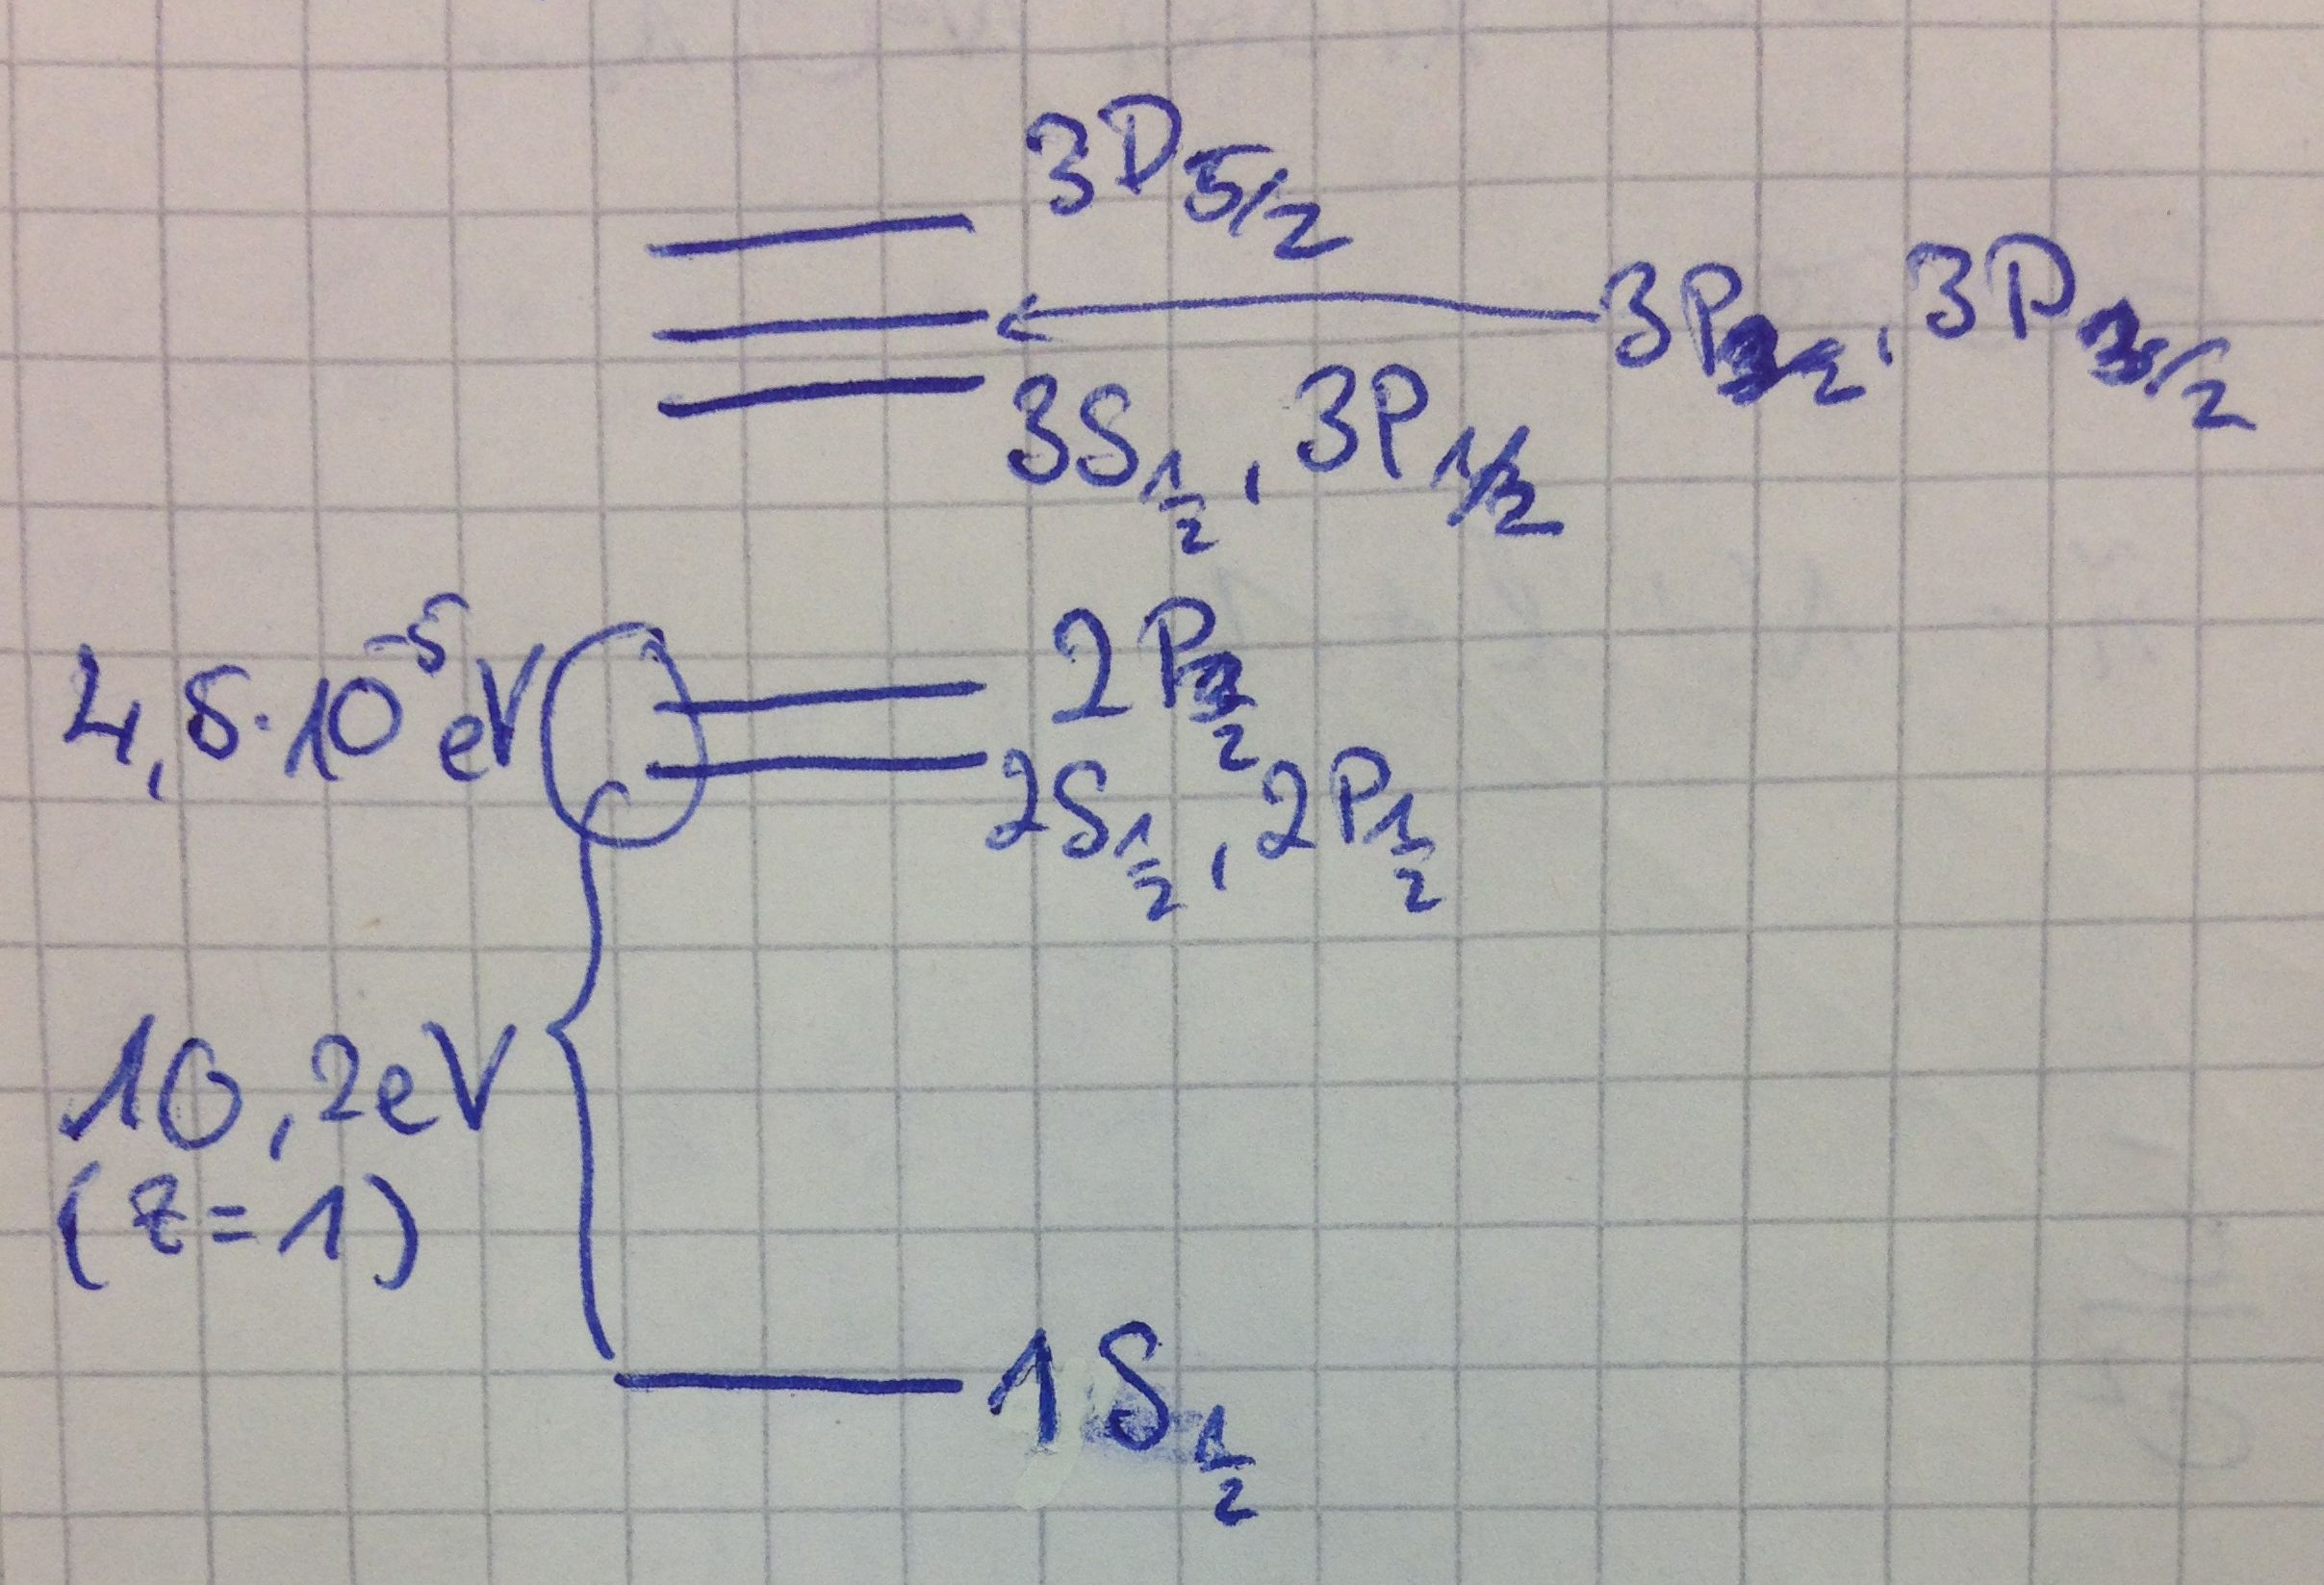
\includegraphics[width=10cm]{Relativistisches_Coulombproblem1}
		\end{center}
	\end{figure*}
Die $j$-Entartung wird beim realistischen Problem aufgehoben durch:
	\begin{itemize}
		\item Wechselwirkung mit magnetischem Moment des Atomkerns: \\
			(Hyperfeinstruktur)
			$\sim 5,8 \cdot 10^{-6} e$V für $ H:~ ^1S_{\frac{1}{2}} \sim \frac{1}{n^2}$ 
		\item Endliche Kernausdehnung 
			$\sim -\frac{1}{n^3} $ für $ H:~ 4\cdot 10^{-1} e$V
		\item Lambshift für $H:~ ^2S_{\frac{1}{2}} / ^2P_{\frac{1}{2}}: ~ 
		4,3 \cdot 10^{-6} e$V \\
			(Effekt des quantisierten elektromagnetischen Feldes, QED)
	\end{itemize}
Problem bei $Z\sim \frac{1}{\alpha} \sim 137$
\\
Konsistene Beschreibung hochionisierter Groß-$Z$-Atome ist nicht im Rahmen einer 1-Teilchen-Theorie möglich (Erzeugung viertueller $e^+e^-$-Paare $\Rightarrow$ QED)
	%Kap5
	\section{Pfadintegrale in der Quantenmechanik}
	\subsection{Übergangsamplituden}
Betrachte eindimensionale Probleme

Mechanik:
	\begin{align*}
		L(x,\dot{x}) &= 
		\frac{m}{2} \dot{x}^2 - V(x),&
		\text{kanonischer Impuls } p&= \frac{\partial L}{\partial \dot{x}}\\
		H(x,p) &= \dot{x}p(x,\dot{x}) - L(x, \dot{x}) = \frac{p^2}{2m} - V(x)
	\end{align*}
	\begin{align*}
		H\ket{n} &= E_n \ket{n} ,& 
		\braket{n | m} &= \delta_{mn} ,& 
		\sum_n \ket{n} \bra{n} &= \mathds{1} \\
		\text{Ortsoperator} \\
		\hat{x} \ket{x} &= x \ket{x} ,&
		\braket{x | x'} &= \delta(x - x') ,&
		\int \diff x \ket{x} \bra{x} &= \mathds{1} \\
		\text{Beliebiger Zustand }
		&\ket{\psi} ,&
		\psi(x) &= \braket{x | \psi} ,&
		\text{insbesondere } \braket{x | n} &= \psi_n(x)
	\end{align*}
Schrödingergleichung
	\begin{align*}
		H \ket{\psi(t)} &= i \hbar \frac{\partial}{\partial t} \ket{\psi(t)}
		& &\Rightarrow \psi(t) = \U_t \ket{\psi(0)} \\
		\text{mit } \U_t &= e^{-\frac{i}{\hbar} H t} & &\text{Unitärer Zeitentwicklungsoperater}
	\end{align*}
(Zeitordung wäre notwenig, falls $V(x,t) t$-abhängig wäre)
	\begin{align*}
		\Rightarrow \ket{x(t)} &= \U_t \ket{x(0)} = \U_t \ket{x} 
	\end{align*}
Übergangselement von Position $x_i$ zur Zeit $t_i$ nach $x_f$ zur Zeit $t_f$ 
	\begin{align*}
		|\braket{x_f | x_i}|^2 :& \text{ Wahrscheinlichkeitsdichte von, wenn ich bei }x_i\text{ starte,}\\ &\text{ komme ich bei }x_f\text{ an} \\
		_H\braket{x_f;t_f | x_i; t_i}_H &=
		\braket{x_f(t_f) | \U_{t_f} \U_{t_i}^\dagger | x_i(t_i)} \\
		&= \braket{x_f(t_f) | \exp \left(-\frac{i}{\hbar} H(t_f-t_i)\right) | x_i(t_i)}\\
		&= \sum_n \braket{x_f | n} \braket{n | x_i} e^{-\frac{i}{\hbar} E_n (t_f - t_i)} \\
		&= \sum_n \psi_n (x_f) \psi^*_n(x_i) e^{-\frac{i}{\hbar} E_n (t_f - t_i)}
	\end{align*}
Übergangsamplitude enthält Information ber Wellenfunktionen $\psi_n(x)$ und Energien $E_n$ 
\\
Alternative Formulierung der Quantenmechanik:

``Pfadintegrale'' erlauben Berechnung von Korrelationsfunktionen (Dirac 1931, Feynman 194..), z.B. $_H\braket{x_f | \hat{x} (t_2) \hat{x} (t_1) | x_i}_H$, ohne dass die Schrödingergleichung gelöst werden muss. 
\\
Diskretisiere die Zeit:
	\begin{align*}
		\ket{x_j}_H &= \ket{x_j ; t_j}_H ,&
		t_j &= j \cdot a ,& t_i &= t_0 = t = 0,&
		t_f &= t_N = Na \\
		\text{mit } a &= \frac{t_f}{N} ,& N &\in \mathds{N}
	\end{align*}
	\begin{figure*} [h]
		\begin{center}
			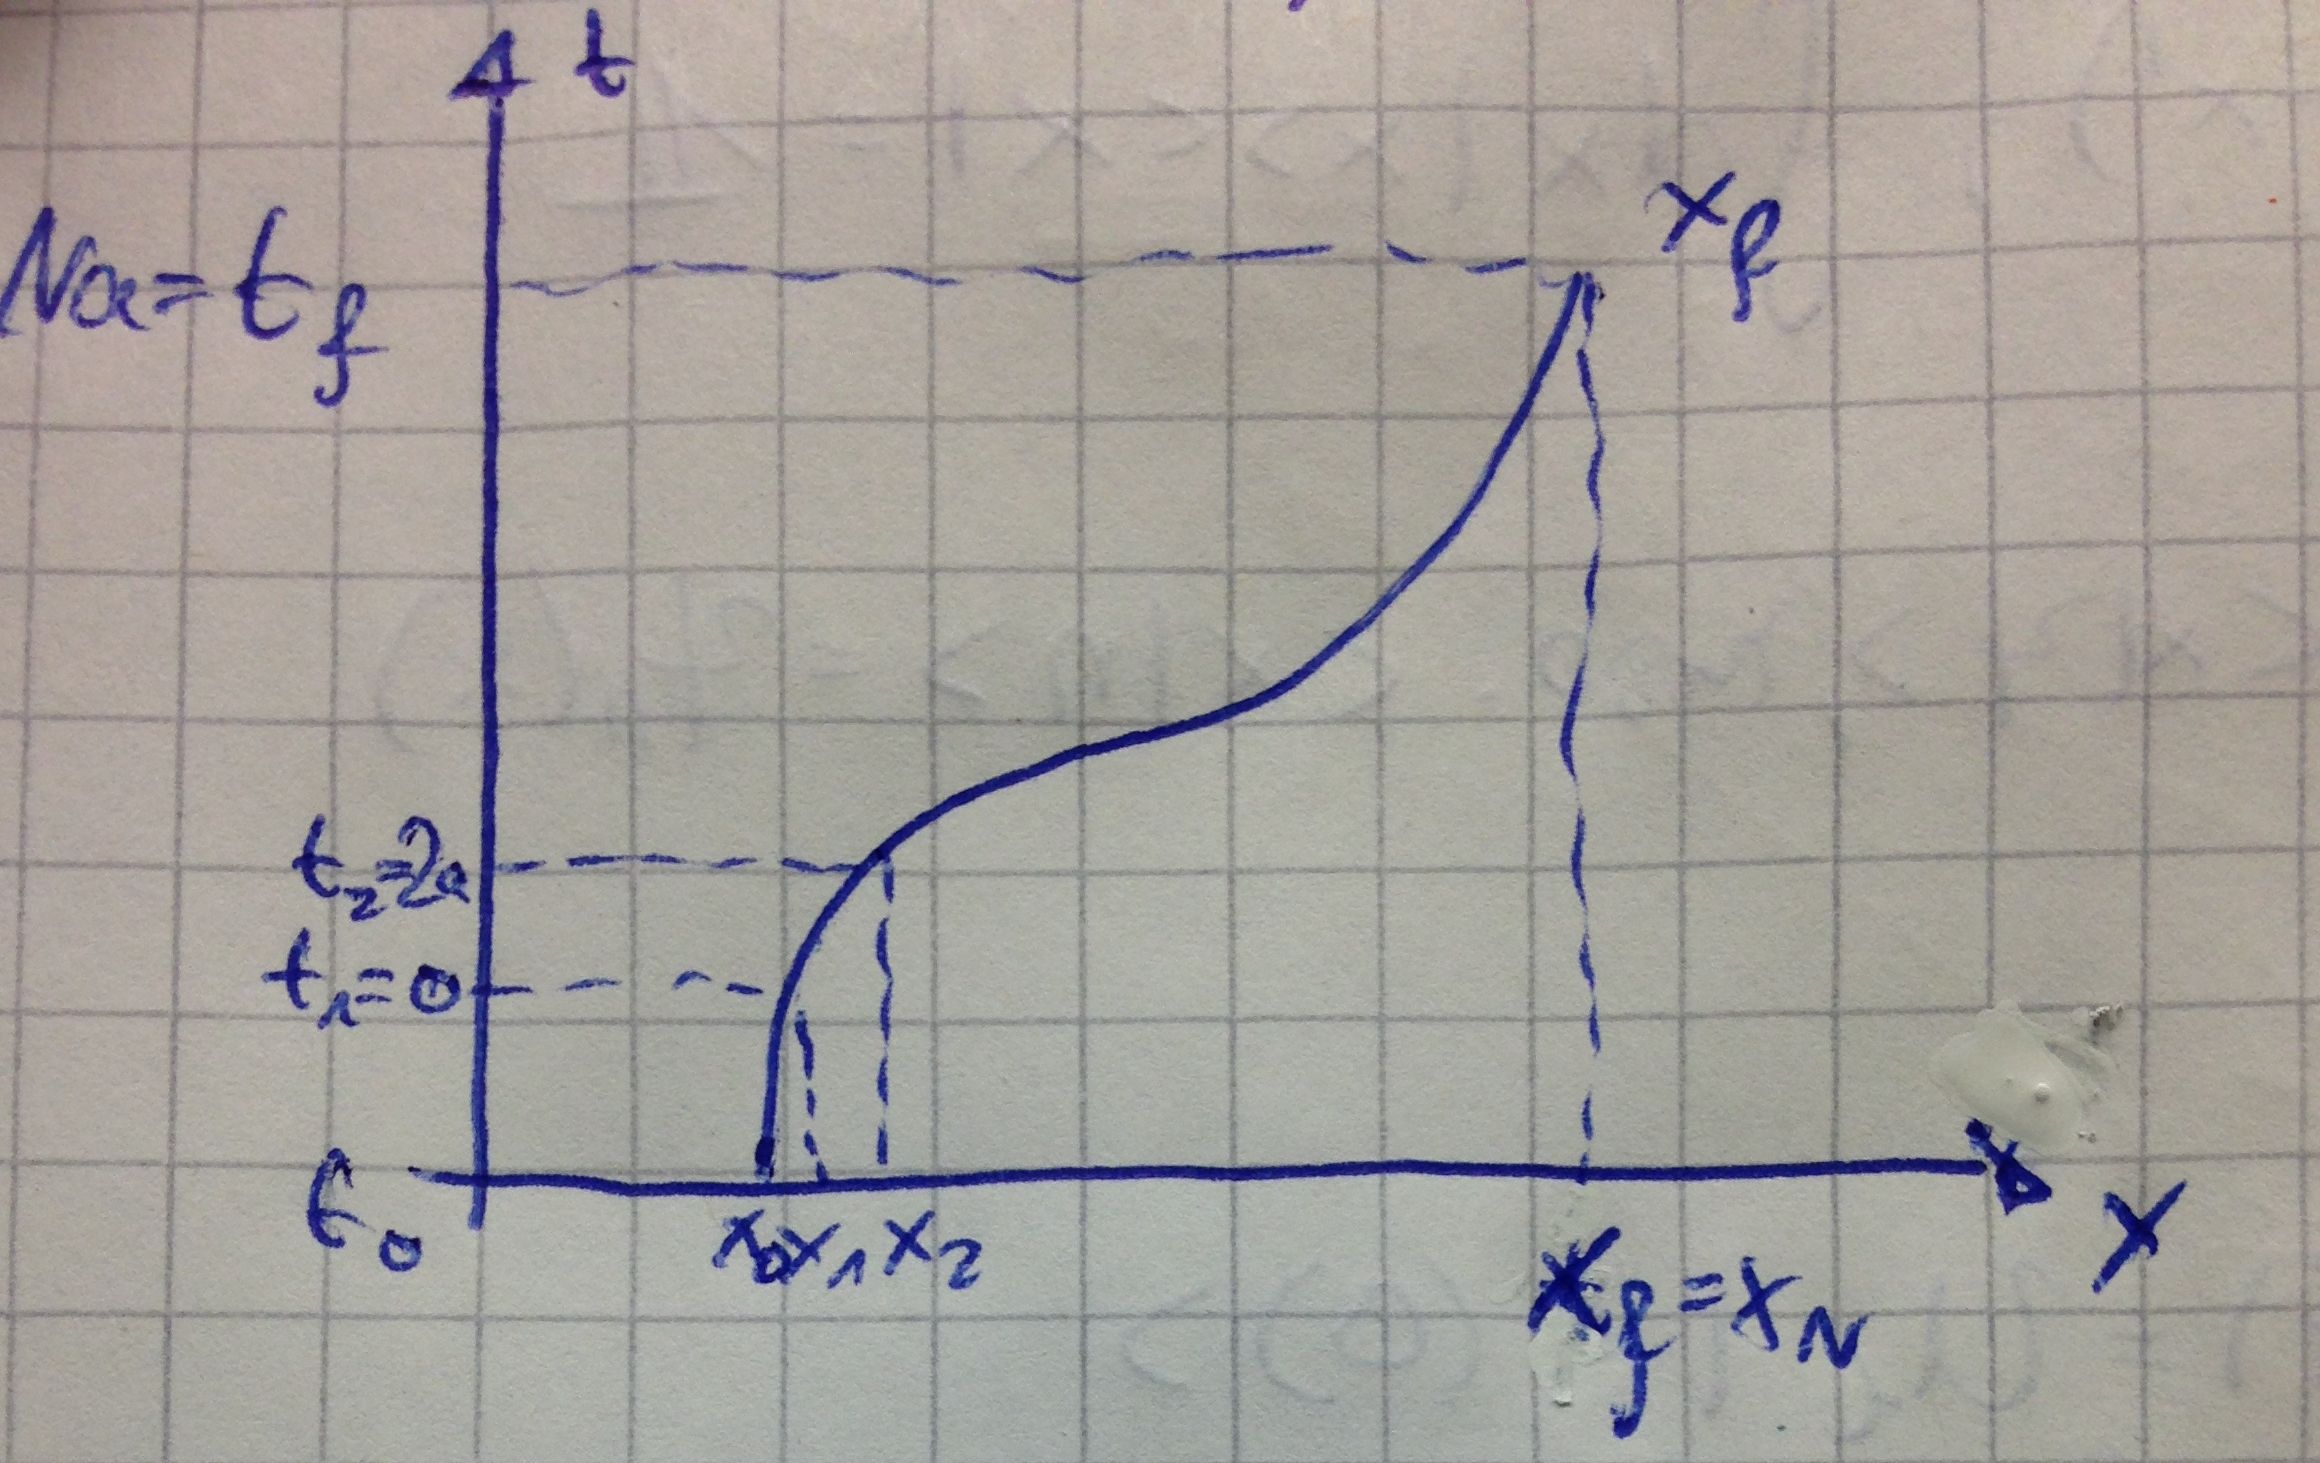
\includegraphics[width=10cm]{Uebergangsamplituden1}
		\end{center}
	\end{figure*}
Setze ein: $\mathds{1} = \int \diff x_j \ket{x_j}_H \vphantom{\bra{x_j}}_H\bra{x_j}$
	\begin{align*}
		&\Rightarrow _H\braket{x_f | x_i}_H^{(N)} 
		\left(\underset{N\rightarrow \infty , a \rightarrow 0}{\longrightarrow} \vphantom{\braket{x_f | x_i}}_H\braket{x_f | x_i}_H\right) \\
		&= \int \vphantom{\braket{x_f | x_i}}_H\braket{x_f | x_{N - 1}}_H \diff x_{N-1} \vphantom{\braket{x_f | x_i}}_H\braket{x_{N-1} | x_{N-2}}_H 
		\diff x_{N-2} \vphantom{\braket{x_f | x_i}}_H\braket{x_{N-2} | \ldots | x_1}_H
		\diff x_1 \vphantom{\braket{x_f | x_i}}_H\braket{x_1 | x_i}_H
	\end{align*} 
Was ist $_H\braket{x_{j+1} | x_j}_H$?

Transferoperator:
	\begin{align*}
		\hat{\mathrm{T}} &= e^{-\frac{i}{\hbar} H a} ,&
		\hat{\mathrm{T}}^N &\approx \U_t
	\end{align*}
	\begin{align*}
		_H\braket{x_{j+1} | x_j}_H &= {}_H\braket{x_{j+1}| \hat{\mathrm{T}} | x_j}_H \\
		&= {}_H \braket{x_{j+1} | e^{-\frac{ia}{\hbar} \left(\frac{\hat{p}^2}{2m} + V(x)\right)} | x_j}_H \\
		&= {}_H \braket{x_{j+1} | e^{-\frac{ia}{2\hbar} V(x_{j+1})} e^{-\frac{ia}{2\hbar}V(x_j)} | x_j}_H (1 + \mathscr{O}(a^2))
	\end{align*}
	\begin{align*}
		_H\braket{x_{j+1} | x_j}_H &=
		{}_H\braket{x_{j+1} | e^{-\frac{ia}{\hbar} \frac{\hat{p}^2}{2m}} | x_j}_H
		e^{-\frac{ia}{\hbar} \left(V(x_j) + V(x_{j + 1})\right)}
	\end{align*}
Füge ein:
	\begin{align*}
		\int \frac{\diff p}{2 \pi} \ket{p} \bra{p} &= \mathds{1} ,& 
		\braket{x | p} &= e^{\frac{i}{\hbar} xp}
	\end{align*}
	\begin{align*}
		_H\braket{x_{j+1} | e^{-\frac{ia}{\hbar} \frac{\hat{p}^2}{2m}}| x_j}_H
		&= \int \frac{\diff p}{2 \pi} e^{\frac{i}{\hbar} (x_{j+1} - x_j)}  e^{-\frac{ia}{\hbar} \frac{\hat{p}^2}{2m}} \\
		&= \sqrt{\frac{m}{2 \pi i a}} \exp\left(\frac{im}{2 \hbar a} (x_{j+1} - x_j)\right)^2 \\
		&= \sqrt{\frac{m}{2 \pi i a}} \exp\left[\frac{ia}{\hbar} \frac{p_j^2}{2m}\right]
		(1 + \mathscr{O}(a^2)) \\
		_H\braket{x_{j+1} | x_j}_H &=
		\sqrt{\frac{m}{2 \pi i a}} e^{\frac{ia}{\hbar} \left[\frac{p_j^2}{2m} - \frac{1}{2} V(x_{j+1}) - \frac{1}{2} V(x_i)\right]} \\
		&\propto \exp (i \frac{a}{\hbar} L_j)
	\end{align*}
\underline{Pfadintegrale} (1.dim) \marginpar{10.12.15}
\marginpar{nicht von Prof.Bali gehalten}
	\begin{figure*} [h]
		\begin{center}
			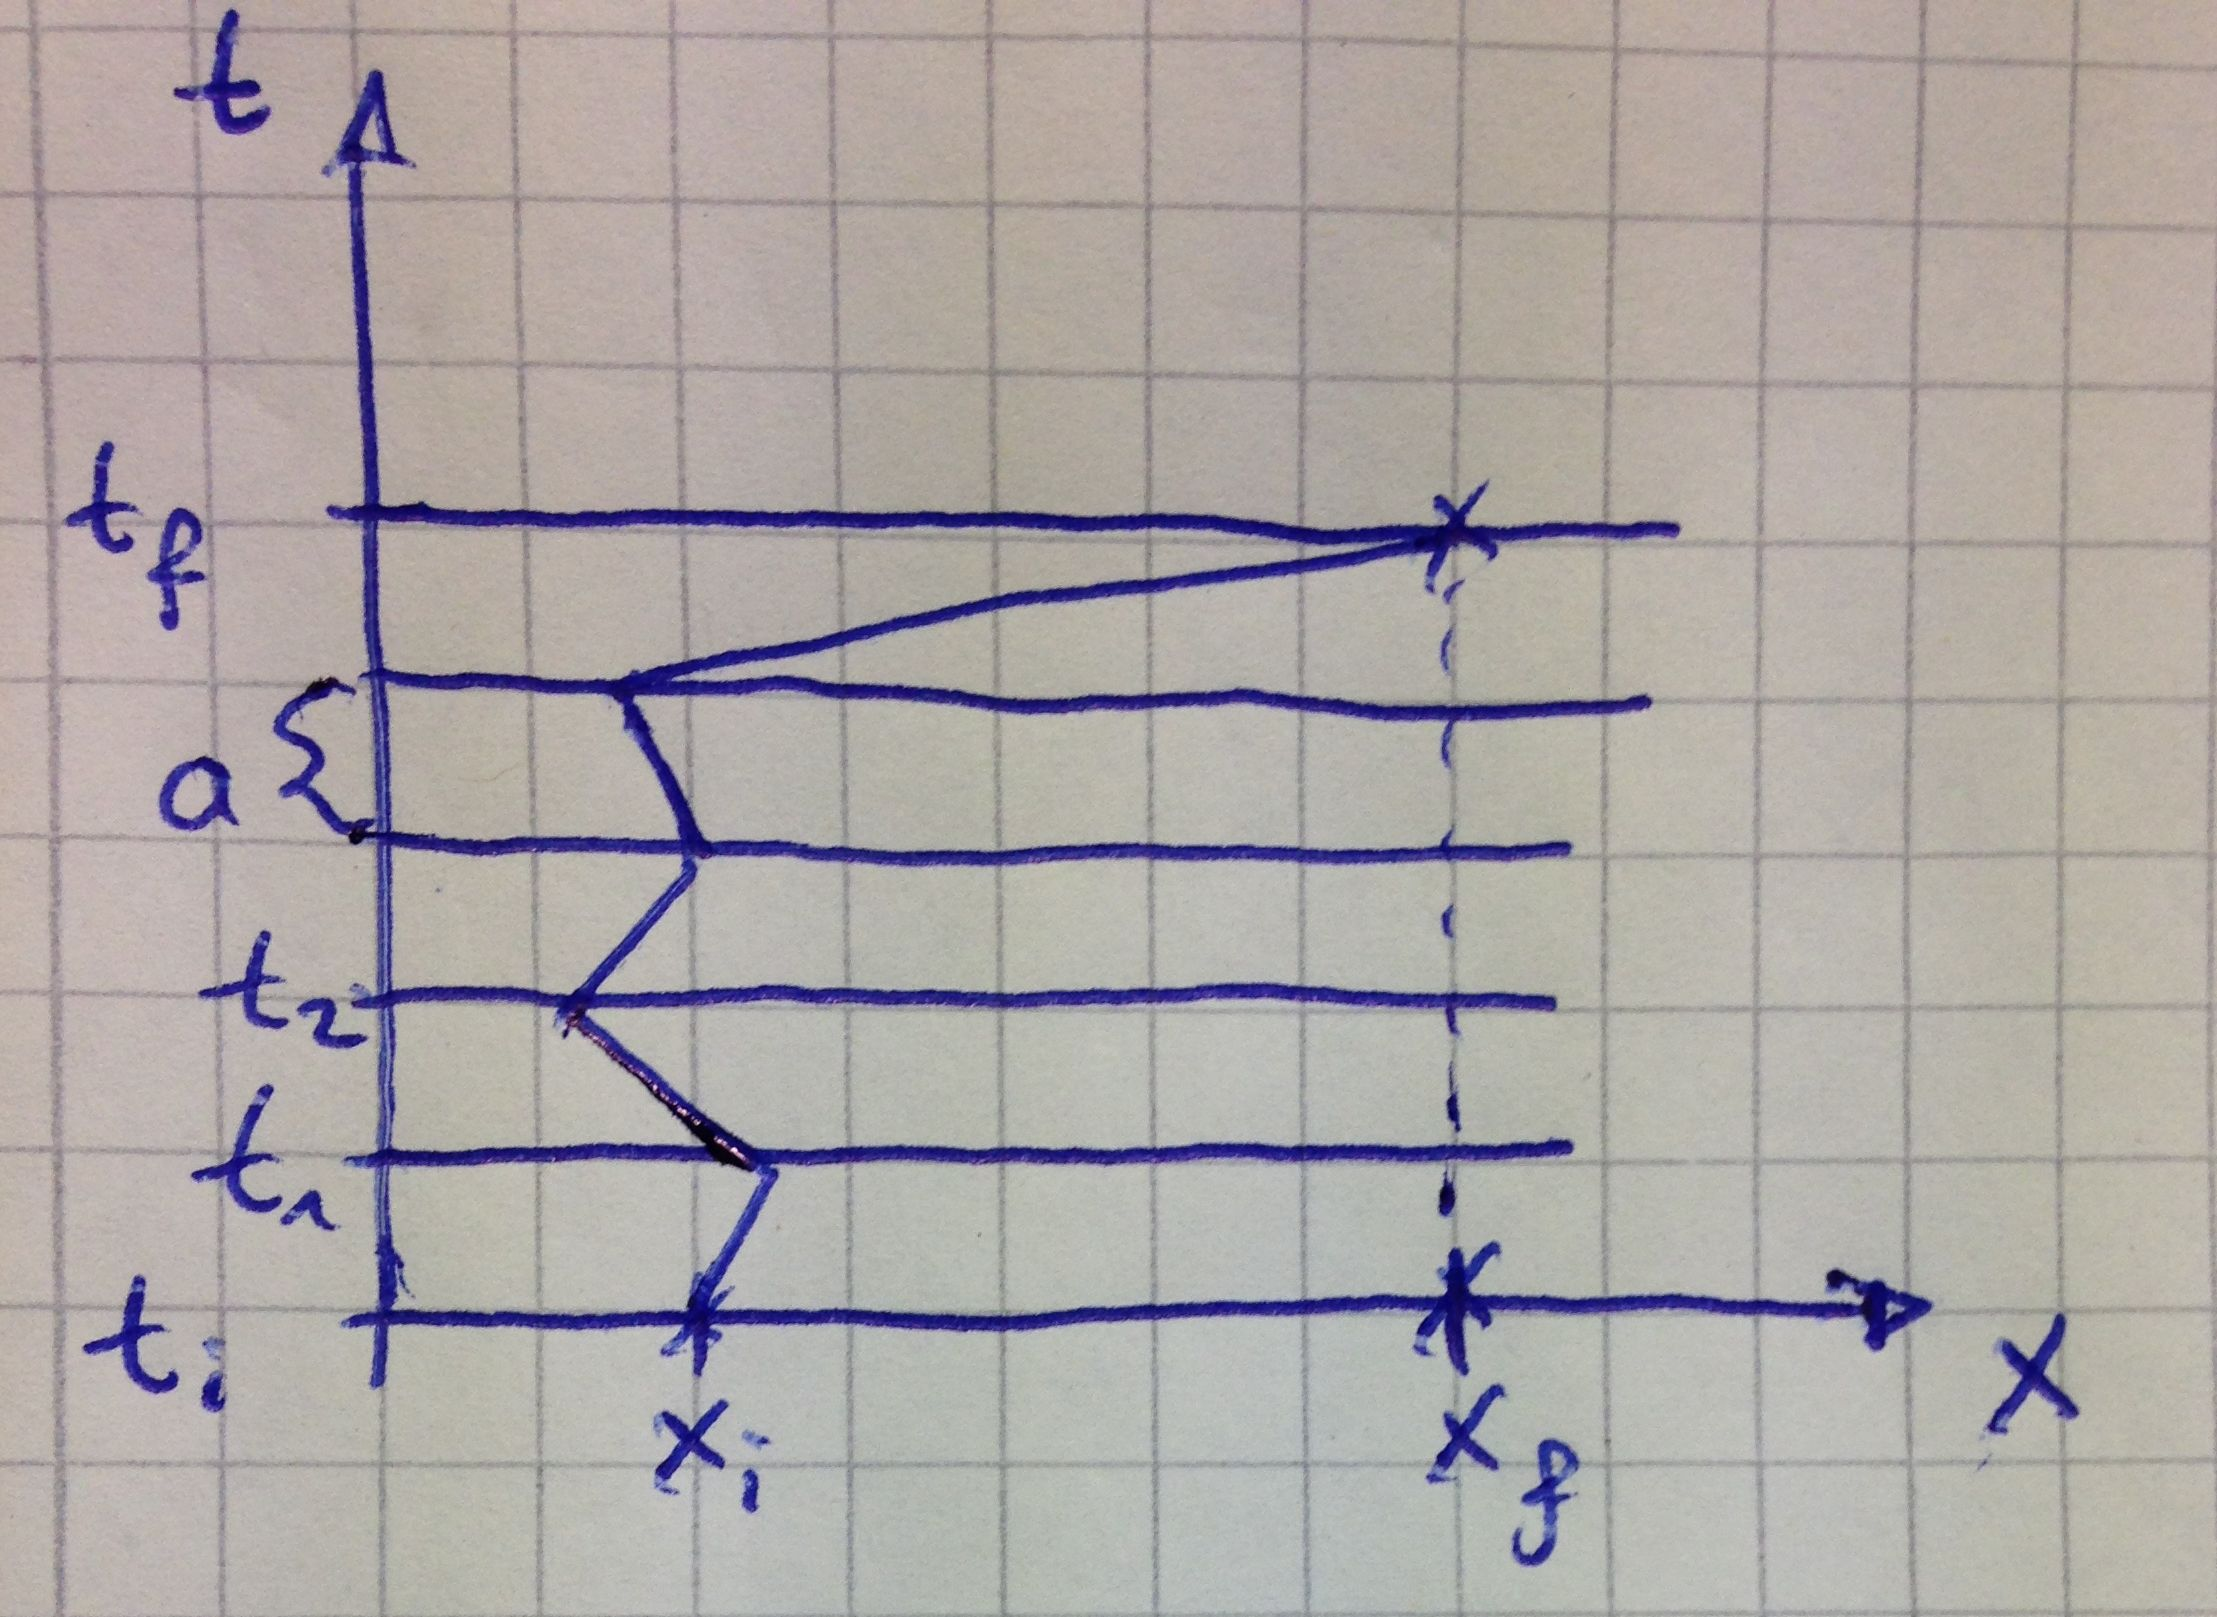
\includegraphics[width=8cm]{Uebergangsamplituden2}
		\end{center}
	\end{figure*}
	\begin{align*}
		\braket{x_f, t_f | x_i , t_i} &=
		\int \diff x_1 \ldots \diff x_{N-1} 
		\braket{x_f, t_f | x_{N-1}, t_{N-1}} 
		\braket{x_{N-1}; t_{N-1}| x_{N-2};t_{N-2}} \\
		&\ldots
		\braket{x_{j+1}, t_{j+1}| x_j, t_j} \\
		\braket{x_{j+1},t_{j+1} | x_j, t_j}
		&= \sqrt{\frac{m}{2\pi\hbar ia}} e^{\frac{ia}{\hbar}} 
		\left[
			\left(m \frac{x_{j+1} - x_j}{a}\right)^2 \frac{1}{2 m}
			-\frac{1}{2} \left(V(x_{j+1}) + V(x_j)\right)
		\right] \\
		&\left(H = \frac{\hat{p}^2}{2m} + V(x)\right) 
	\end{align*}
$a \rightarrow 0,~ N \rightarrow \infty,~ aN = t_f - t_i$
	\begin{align*}
		\Rightarrow& \braket{x_f,t_f | x_i,t_i} =
		\sqrt{\frac{m}{2 \pi i a \hbar}}^N 
		\int \prod_i \diff x_i e^{\frac{i}{\hbar} \sum_i a L_i} \\
		&\rightarrow \int [dx] e^{\frac{i}{\hbar} \int \diff t L} 
		& S &= \int \diff t L
	\end{align*}
$S$ ist Funktional : $S[x(t)] = $ Zahl
	\begin{align*}
		\braket{x_f,t_f | x_i,t_i} &= \int [\diff x] e^{\frac{i}{\hbar} S[x]} \\
		S &= \int \limits_{t_i}^{t_f} \diff t L[x(t)]
	\end{align*} 
wenn $S \gg \hbar$.

fluktuiert die Phase stark, Beiträge in diesem Term (zu diesem Pfad) klein.
\\
Der Hauptbeitrag kommt von Pfaden, in denen $S$ möglichst klein ist. 
\\
$\rightarrow$ Prinzip der minimalen Wirkung

Funktionales Differenzieren:
	\begin{align*}
		F[f]& &
		\frac{\delta F}{\delta f(y)} &=
		\lim\limits_{\epsilon \rightarrow 0} 
		\frac{F\left(f(x) + \epsilon \delta(x-y)\right) - F[f(x)]}{\epsilon} \\
		F[f] &= \int \diff x g(x) f(x) 
	\end{align*}
	\begin{align*}
		\frac{\delta F}{\delta f(y)} &= 
		\lim\limits_{\epsilon \rightarrow 0}
		\int \frac{\diff x g(x) [f(x) + \epsilon \delta(x-y) - f(x)]}{\epsilon} 
		= g(y) \\
		\frac{\delta S[x]}{\delta x(t)} &=
		\lim\limits_{\epsilon \rightarrow 0} \frac{1}{\epsilon}
		\left(
			\int \diff t' \left(\frac{1}{2} m \frac{\diff}{\diff t'} \left(x(t') + \epsilon \delta(t-t')\right)\right)
		\right)^2 \\
		&- V(x + \epsilon \delta(t-t')) - \int \diff t \left(\frac{1}{2} m \dot{x}^2 - V(x)\right) \\
		&\overset{\epsilon^2 \rightarrow 0}{=}
		\int \diff t'
		\left(
			m \frac{\diff x}{\diff t} \frac{\diff (\delta(t-t'))}{\diff t} 
			- \frac{\partial V}{\partial x} \delta(t-t')
		\right) \\
		&= \int \diff t'
		\left(
			- m \frac{\diff^2 x}{\diff t^2} - \frac{\partial V}{\partial x}
		\right) \delta(t'- t)
	\end{align*}
	\begin{align*}
		\frac{\delta S}{\delta x} = 0 &\Longleftrightarrow 
		m \frac{\diff^2 x}{\diff t^2} = - \frac{\partial V}{\partial x} \\
		\int\limits_{-\infty}^\infty \diff x e^{-x^2} &= \sqrt{\pi} \\
		\int\limits_{-\infty}^\infty e^{-ax^2 + bx + c} &=
		\exp \left(\frac{b^2}{4a} + c\right) \left(\frac{\pi}{a}\right)^{\frac{1}{2}}
	\end{align*}
$a \neq 0,~ \mathrm{Re} ~a \geq 0$ \\
Freie Teilchen, $V=0$
	\begin{align*}
		&\left(\frac{m}{2 \pi i \hbar a}\right)^{\frac{3}{2}}
		\int\limits_{-\infty}^\infty \diff x_1 \exp 
		\left(
			\frac{im}{2\hbar a} \left[
				(x_2 - x_1)^2 + (x_1 - x_0)^2
			\right]
		\right) \\
		&= \left(\frac{m}{2\pi i \hbar 2 a}\right)^{\frac{1}{2}}
		\exp \left(
			\frac{im}{2 \hbar 2 a} (x_2 - x_0)^2
		\right)
	\end{align*}
nächster Schritt: Integration über $x_2$
	\begin{align*}
		\left(\frac{m}{2 \pi i \hbar 3 a}\right)^{\frac{1}{2}}
		\exp \left(
			\left(\frac{im}{2\hbar 3 a}\right) (x_3 - x_0)^2
		\right)
	\end{align*}
nach $N$ Schritten:
	\begin{align*}
		\braket{x_f,t_f | x_i; t_i} &=
		\left(\frac{m}{2 \pi i \hbar (t_f -t_i)}\right)^{\frac{1}{2}}
		\exp \left(\frac{im (x_f - x_i)^2}{2 \hbar (t_f - t_i)}\right)
	\end{align*}
Dies ist das Ergebnis für freies Teilchen.

	\subsection{Harmonischer Oszillator}
	\begin{align*}
		S = \int \diff t \left(
			\frac{m}{2} \dot{x}^2 - \frac{1}{2} m \omega^2 x^2
		\right)
	\end{align*}
QM: Betrachte Summe über alle Pfade von $x_i \rightarrow x_f$ 

klassische Lösung:
	\begin{align*}
		x_c(t) = x_i \frac{\sin (\omega(t_f - t))}{\sin (\omega(t_f - t_i))}
		+ x_f \frac{\sin (\omega(t - t_i))}{\sin (\omega (t_f - t_i))} 
	\end{align*}
Einsetzen von $x_c$ in Wirkungsfunktional 
	\begin{align*}
		S_c &= \frac{1}{2} m \omega 
		\left(
			\frac{(x_i^2 + x_f^2) \cos(\omega(t_f - t_i)) - 2 x_ix_f}{\sin(\omega(t_f - t_i))}
		\right) \\
		x(t) &= x_c(t) + y(t) \\
		y(t) &\text{ ist Quantenfluktuation und es gilt: } y(t_i) = y(t_f) = 0 \\
		S[x(t)] &= \underbrace{S[x_c]}_{\mathclap{S_c}} + 
		(\text{linearer Term } = 0) +
		\underbrace{\frac{m}{2} \int\limits_0^T \diff t \left(\dot{y}^2 - \omega^2 y^2\right)}_{\mathclap{= \frac{m}{2} \int\limits_0^T \diff t~ y(t)\left(-\frac{\diff^2}{\diff t^2} - \omega^2\right)y}}
	\end{align*}
Entwickle $y$ in Eigenfunktionen von $-\frac{\diff^2}{\diff t^2} - \omega^2$
	\begin{align*}
		y_n &= \sqrt{\frac{2}{T}} \sin \left(\frac{n \pi t}{T}\right) \\
		\int\limits_{0}^T \diff t~y_n(t) y_m(t) &= \delta_{nm} \\
		y(t) &= \sum\limits_{n=1}^\infty a_n y_n(t) 
	\end{align*}
Eigenwerte: $\lambda_n=\frac{n^2 \pi^2}{T^2} - \omega^2$
	\begin{align*}
		&\int [\diff x] e^{\frac{i}{\hbar} S_c} e^{\frac{i}{\hbar} S[y]} \\
		&[dx] \rightarrow [dy] \rightarrow [d a_n] \\
		&S[y] = \sum_{n = 1}^{\infty} \frac{m}{2} \lambda_n a_n^2 \\
		&\text{kann wieder à la Gauß integriert werden}
	\end{align*}
	\begin{align*}
		\braket{x_f, T | x_i, 0} 
		&= const. \int \prod \diff a_1 \exp\left(\frac{i}{\hbar} \frac{m}{2} \sum_{1}^{\infty} \lambda_n a_n^2\right) \\
		&= const. \prod_{n=1}^{\infty}
		\left[
			\frac{m}{2 \pi i \hbar} \lambda_n
		\right]^{\frac{1}{2}} \\
	\end{align*}
freies Teilchen (Grenzfall $\omega \rightarrow 0$):
	\begin{align*}
		\lambda_n^{(0)} &= \frac{n^2 \pi^2}{T^2} \\
		\prod_{n=1}^{\infty} \left(\frac{\lambda_n}{\lambda_n^0}\right)^{-\frac{1}{2}} &=
		\prod_{n=1}^{\infty} \left(1 - \frac{n^2 \pi^2}{T^2}\right)^{-\frac{1}{2}}
	\end{align*}
Durch Vergleich mit $\omega \rightarrow 0$
	\begin{align*}
		\left(\frac{m \omega}{2 \pi i \hbar \sin(\omega T)}\right) &= 
		\braket{x_f , T | x, 0}
	\end{align*}
für $\omega \rightarrow 0$ Vorfaktor $\left(\frac{m}{2 \pi i \hbar T}\right)$

Richtiges Ergebnis für ein freies Teilchen, welches von $x_i = 0$ nach $x_f = 0$ läuft ($y(t_i)= y(t_f) = 0$) 
	\begin{align*}
		E_n = \hbar \omega\left(n + \frac{1}{2}\right)
	\end{align*}
Wellenfunktionen lassen sich alle aus den Matrixelementen $\braket{x_f, T | x_i , 0}$ extrahieren.
\\
Numerische Simulation von Pfadintegralen
	\begin{enumerate}[1)]
		\item endliches $a$ (Gitterabstand) 
		\item endliches Volumen
		\begin{align*}
			\text{Extrapoliere }& &
			\begin{aligned}
				a &\rightarrow 0 \\
				V &\rightarrow \infty
			\end{aligned}
			& &t_i
		\end{align*}
	\end{enumerate}
fragt mich nicht, was das letzte heißt, keine Ahnung


	\subsection{Der Aharanov-Bohn-Effekt} (5.3)\marginpar{14.12.15}
(Ehrenberg-Siday 1949, (wieder entdeckt bzw mathematisch besser:)Aharanov-Bohn 1959)
%	\begin{figure*} [h]
%	\begin{center}
%		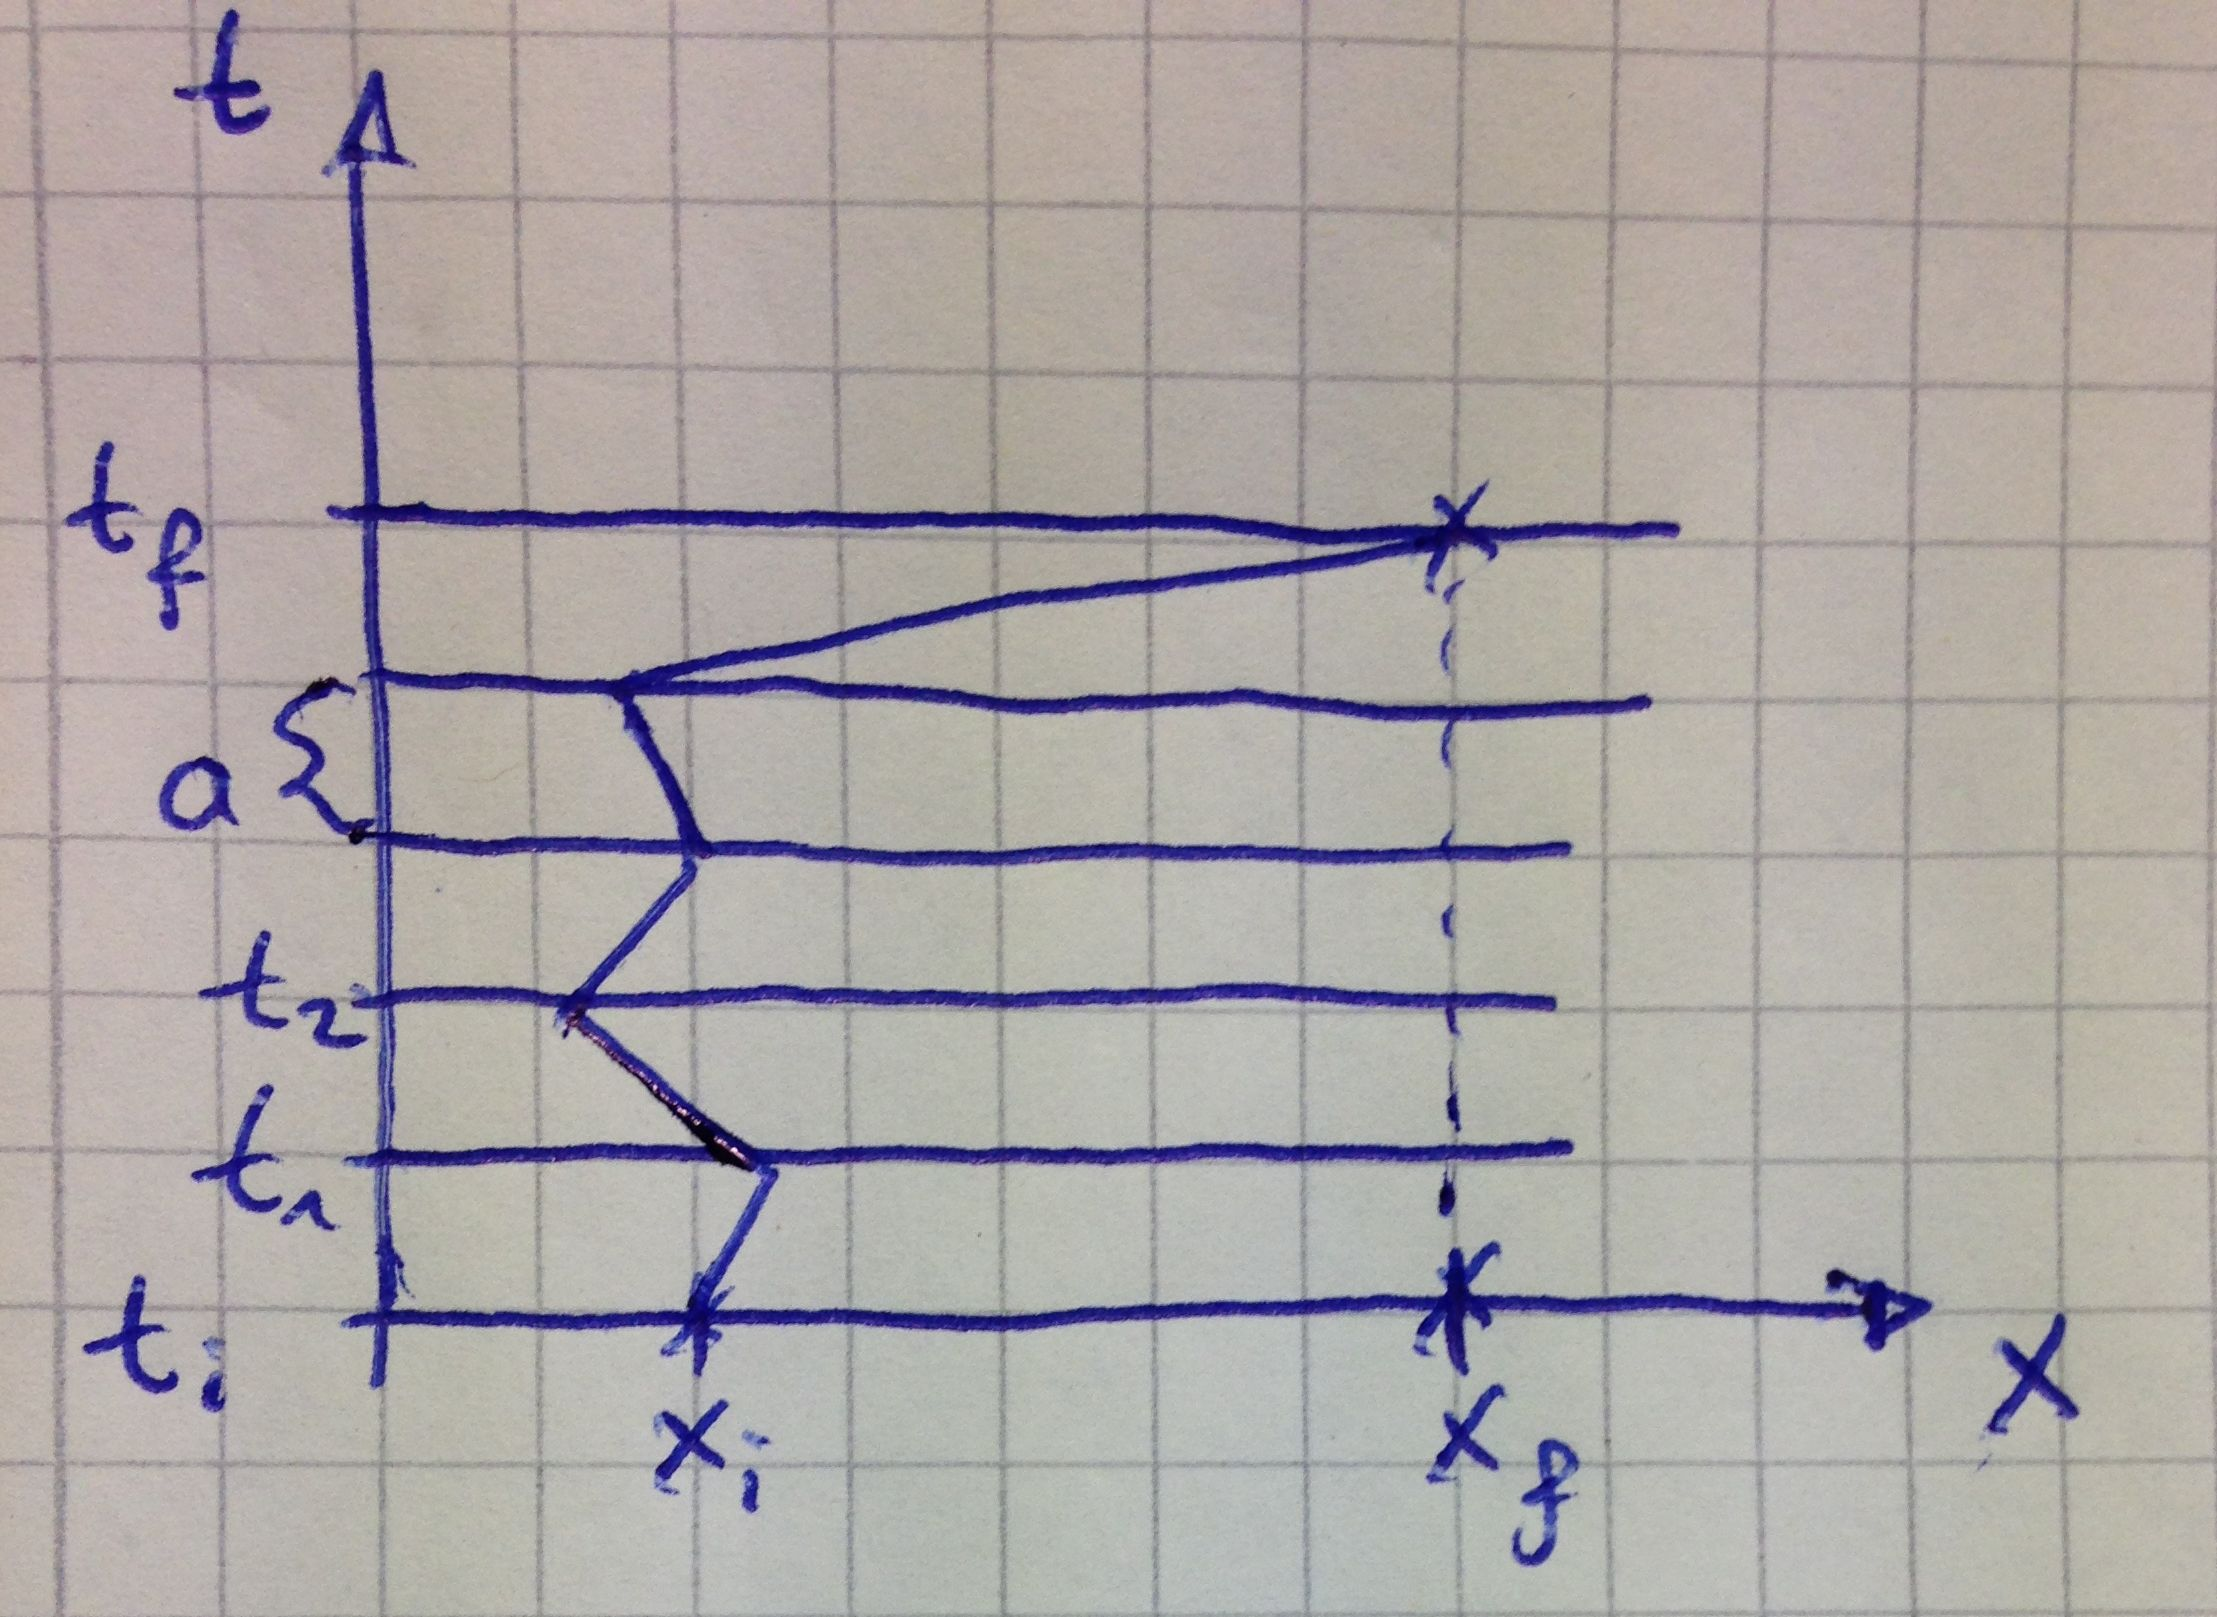
\includegraphics[width=10cm]{Uebergangsamplituden2}
%	\end{center}
%	\end{figure*} bild1
Behauptung: $\vec{B}$ beeinflusst Interferenzmuster

Klassische Physik:
	\begin{align*}
		m \ddot{\vec{r}} &= \frac{q}{c} \dot{\vec{r}} \times \vec{B} \\
		\vec{B} &= \vec{\nabla} \times \vec{A}
	\end{align*}
Beispiel:
	\begin{align*}
		\vec{A}(\vec{r}) &= \frac{\Phi m}{2\pi} \frac{(-y,x,0)}{x^2 + y^2} \\
		\int \diff x \diff y \vec{e}_z \cdot \vec{B}(x,y,z) &=
		\oint_{\partial F} \diff \vec{r} \cdot \vec{A}(\vec{r})=
		\int_{0}^{2 \pi} \diff \phi ~r_{\perp} \frac{\Phi m}{2 \pi} \frac{r_{\perp}}{r_{\perp}^2} \vec{e}_\phi \cdot \vec{e}_\phi \\
		&=\Phi_m ~\text{für jedes } r_{\perp} > 0
	\end{align*}
$\Phi_m$: Magnetisscher Fluß (durch $F$)
	\begin{align*}
		\vec{B} &= \vec{e}_z \cdot \Phi_m \delta^{(3)}(x,y) \\
		\text{Weil } \int_F \diff \vec{f} \cdot \vec{B} &= \Phi_m,&
		\text{Aber } \vec{\nabla} \times \vec{A} \text{ divergiert für } r_{\perp} \rightarrow \infty
	\end{align*}
$\vec{B} = 0$, außer bei $x=y=0$. Aber $\vec{A}(\vec{r}) \neq \vec{0}$ überall.

$\vec{A}(\vec{r})$ ist nur festgelegt bis auf eine Eichtransformation:
	\begin{align*}
		\vec{A} \mapsto \vec{A} + \vec{\nabla} \Lambda (\vec{r}(t)) 
		\Rightarrow \vec{B}(\vec{r}) \mapsto \vec{B}(\vec{r})
	\end{align*}
Lagrangefunktion:
	\begin{align*}
		L &= \frac{m}{2} \dot{\vec{r}}^2 + \frac{q}{c} \dot{\vec{r}} \cdot \vec{A}
		& \frac{\diff}{\diff t} \frac{\partial L}{\partial \dot{r}_i} - \frac{\partial L}{\partial r_i} &= 0 &
		\Rightarrow m \ddot{\vec{r}} &= \frac{q}{c} (\dot{\vec{r}} \times(\vec{\nabla} \times \vec{A})) \\
		&= L_0 + \frac{q}{c} \dot{\vec{r}} \cdot \vec{A}
	\end{align*}
	\begin{align*}
		S &= S_0 + \frac{q}{c} \int_{t_0}^{t_1} \diff t ~\dot{\vec{r}} \cdot \vec{A}(\vec{r}(t)) \\
		&= S_0 + \frac{q}{c} \int_{\vec{r}(t_0) = \vec{y}}^{\vec{r}(t_1) = \vec{x}} \diff \vec{r} \cdot \vec{A}(\vec{r}) 
	\end{align*}
$\vec{A}(\vec{r}) \neq \vec{\nabla}$ (Skalarfeld)(Problem bei $x=y=0$), deshalb wird das zweite Integral wegabhängig sein
	%	\begin{figure*} [h]
	%	\begin{center}
	%		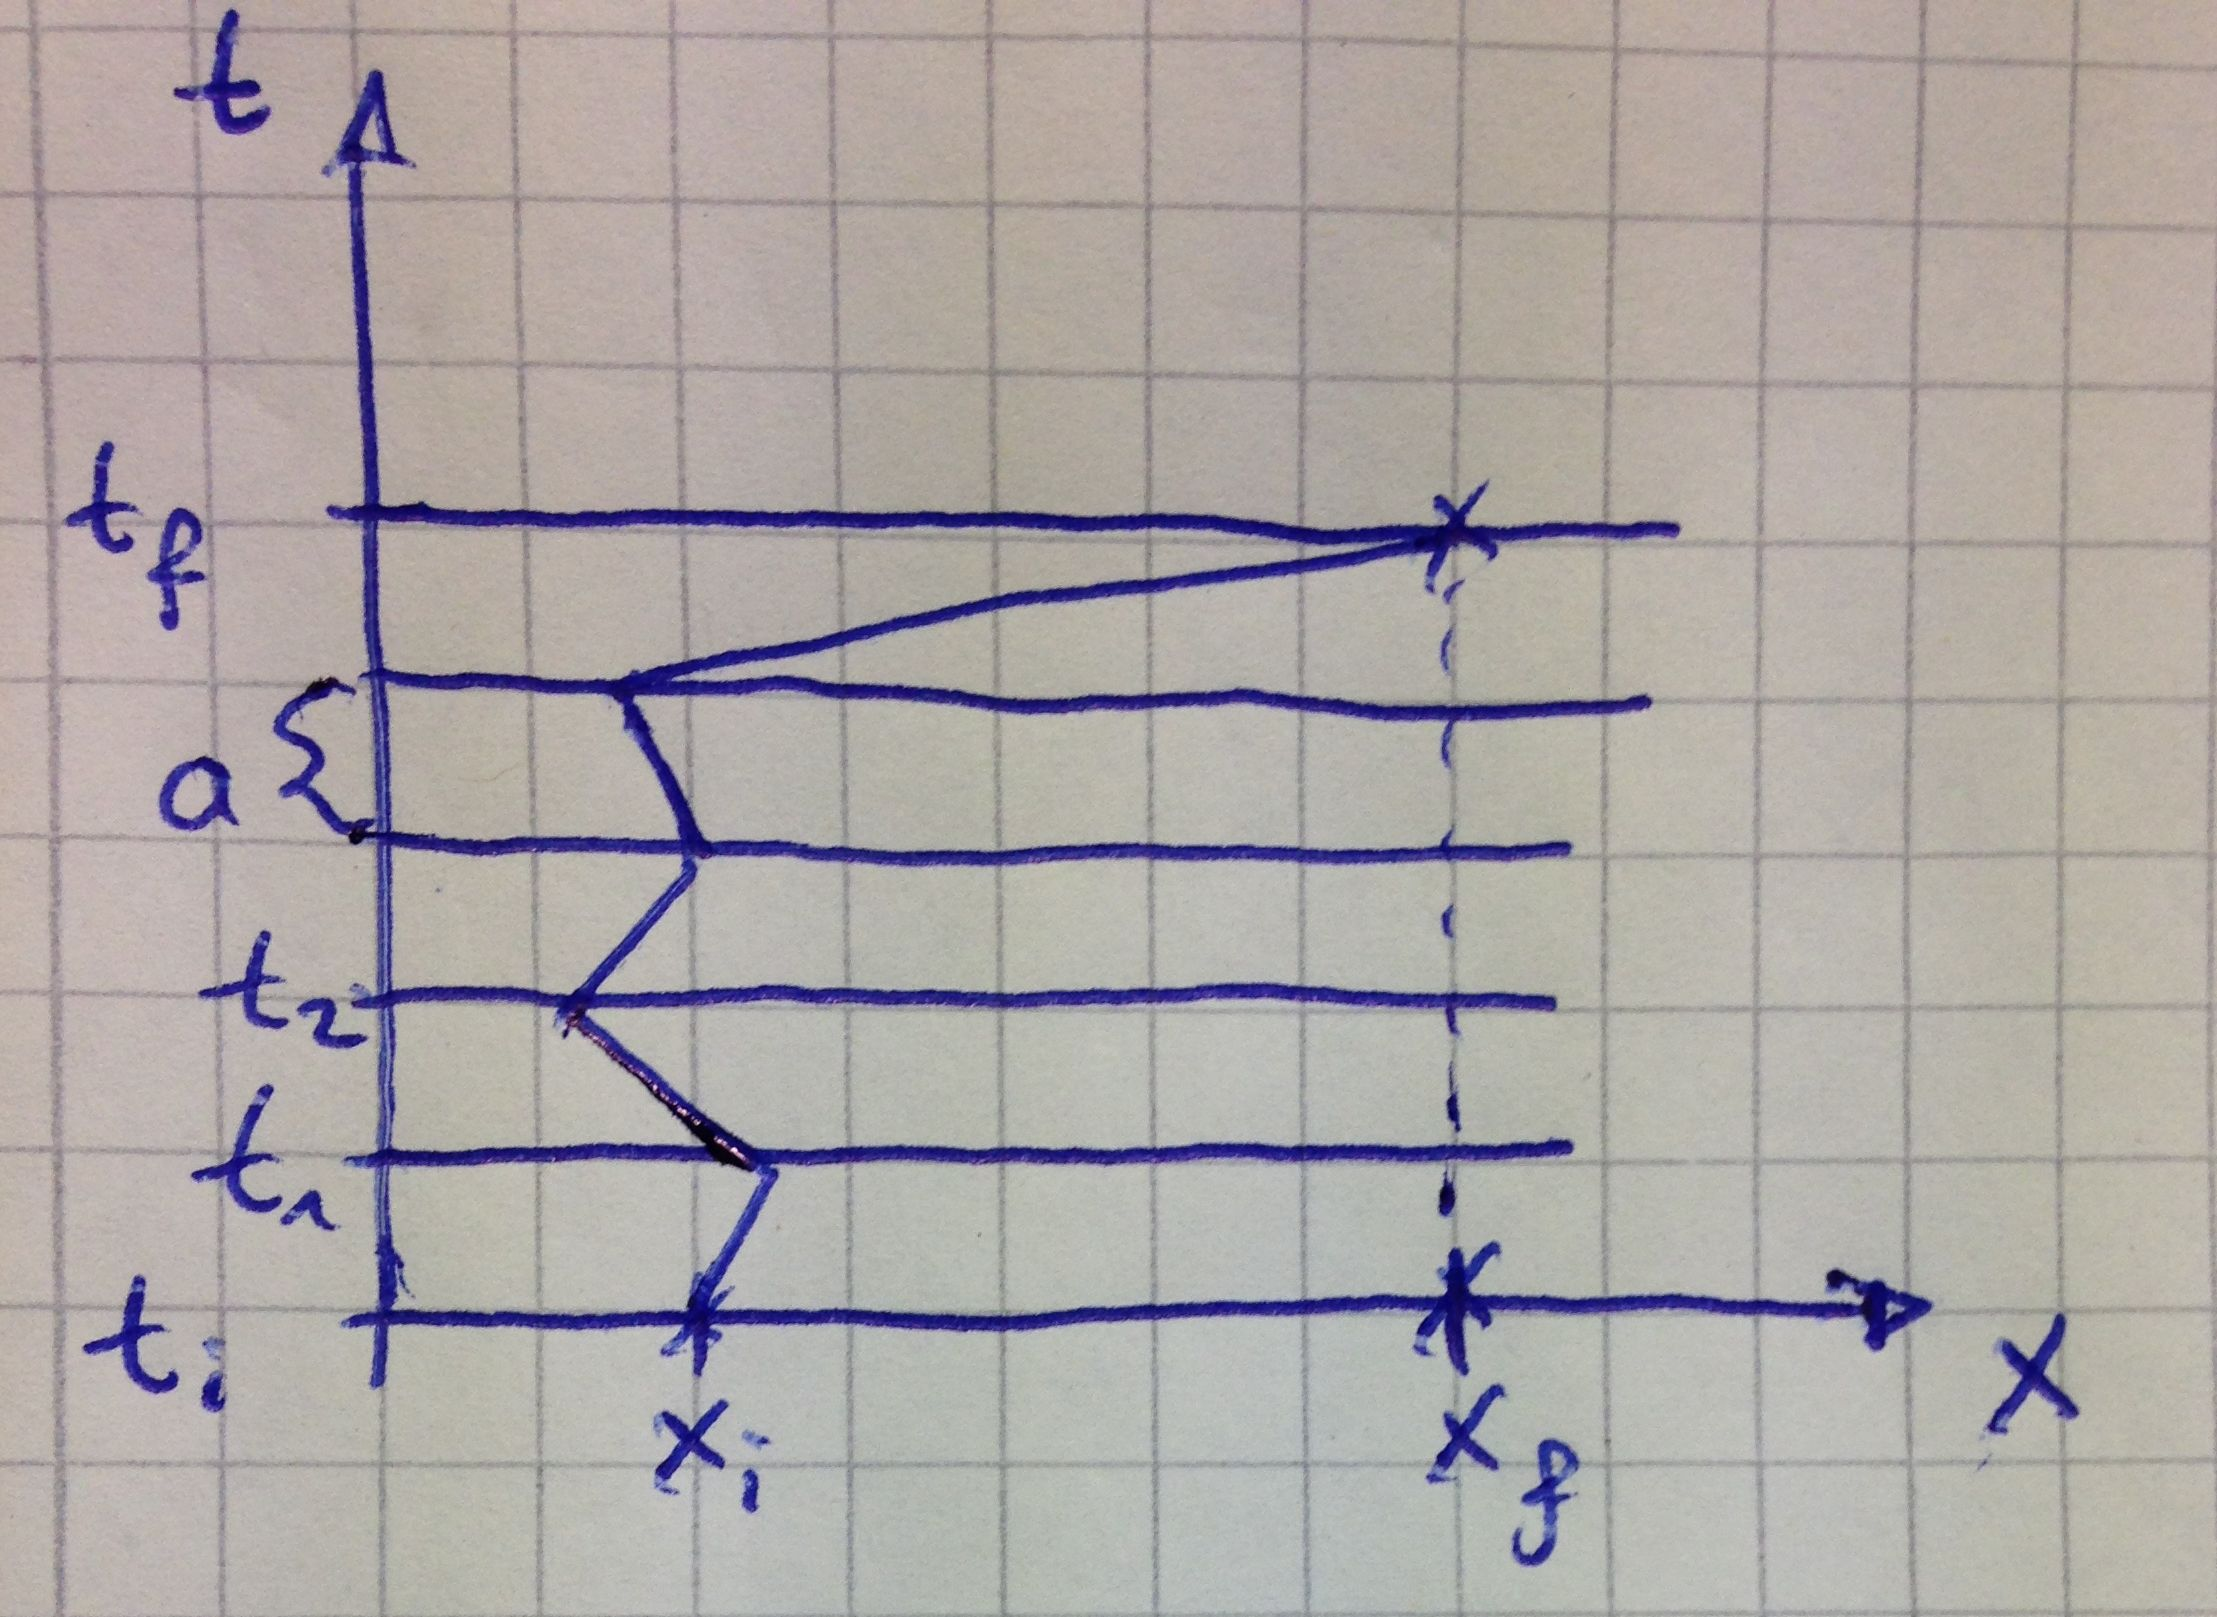
\includegraphics[width=10cm]{Uebergangsamplituden2}
	%	\end{center}
	%	\end{figure*} bild2
	\begin{align*}
		\int_{c_a} \diff \vec{r} \cdot \vec{A}(\vec{r}) - \int_{c_b} \diff \vec{r} \cdot \vec{A}(\vec{r}) &=
		\oint_{c_a-c_b} \overset{Stokes}{=} 
		\int_F \diff \vec{f} (\vec{\nabla} \times \vec{A}) = \int_F \diff \vec{f} \cdot \vec{B}(\vec{r}) =0 \\
		&\Rightarrow 
		\int_{c_a} \diff \vec{r} \vec{A}(\vec{r}) = \int_{c_b} \diff \vec{r} \vec{A}(\vec{r}) =
		\alpha_1 = \int_{c^{(1)}} \diff \vec{r} \cdot \vec{A}(\vec{r})
	\end{align*}
	%	\begin{figure*} [h]
	%	\begin{center}
	%		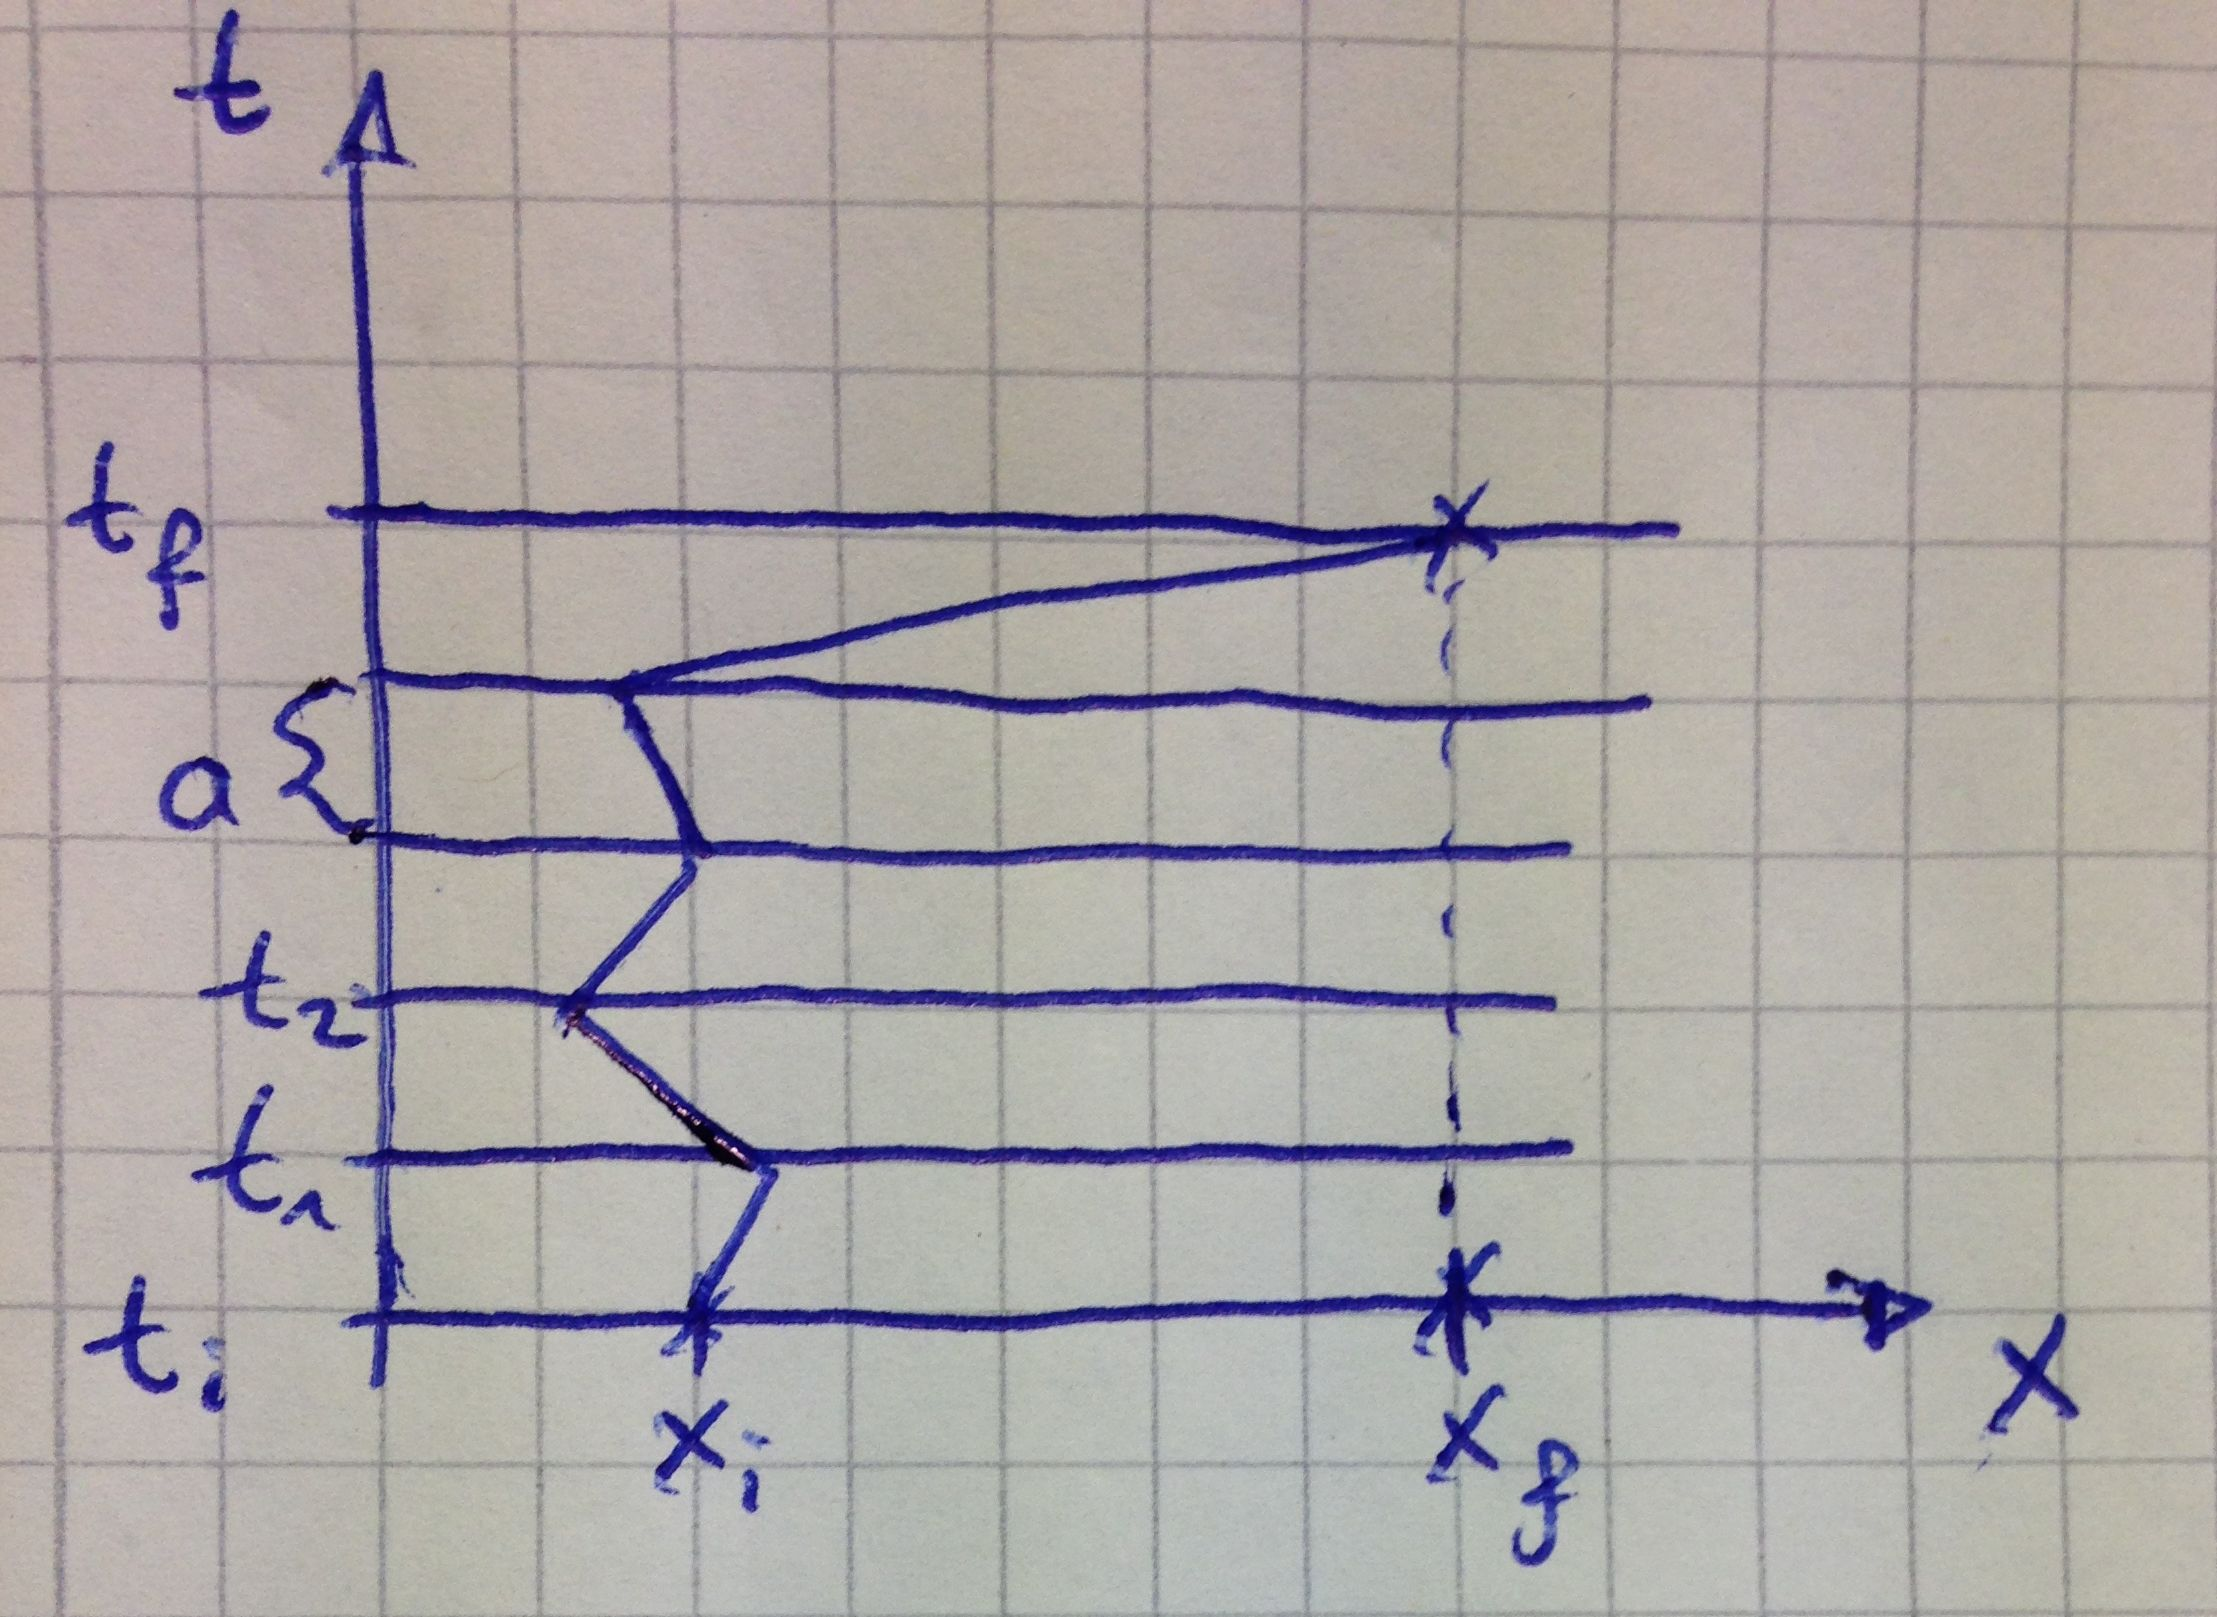
\includegraphics[width=10cm]{Uebergangsamplituden2}
	%	\end{center}
	%	\end{figure*} bild3
	\begin{align*}
		\int_{c^{(2)}} \diff \vec{r} \vec{A}(\vec{r}) = \alpha_2
	\end{align*}
	%	\begin{figure*} [h]
	%	\begin{center}
	%		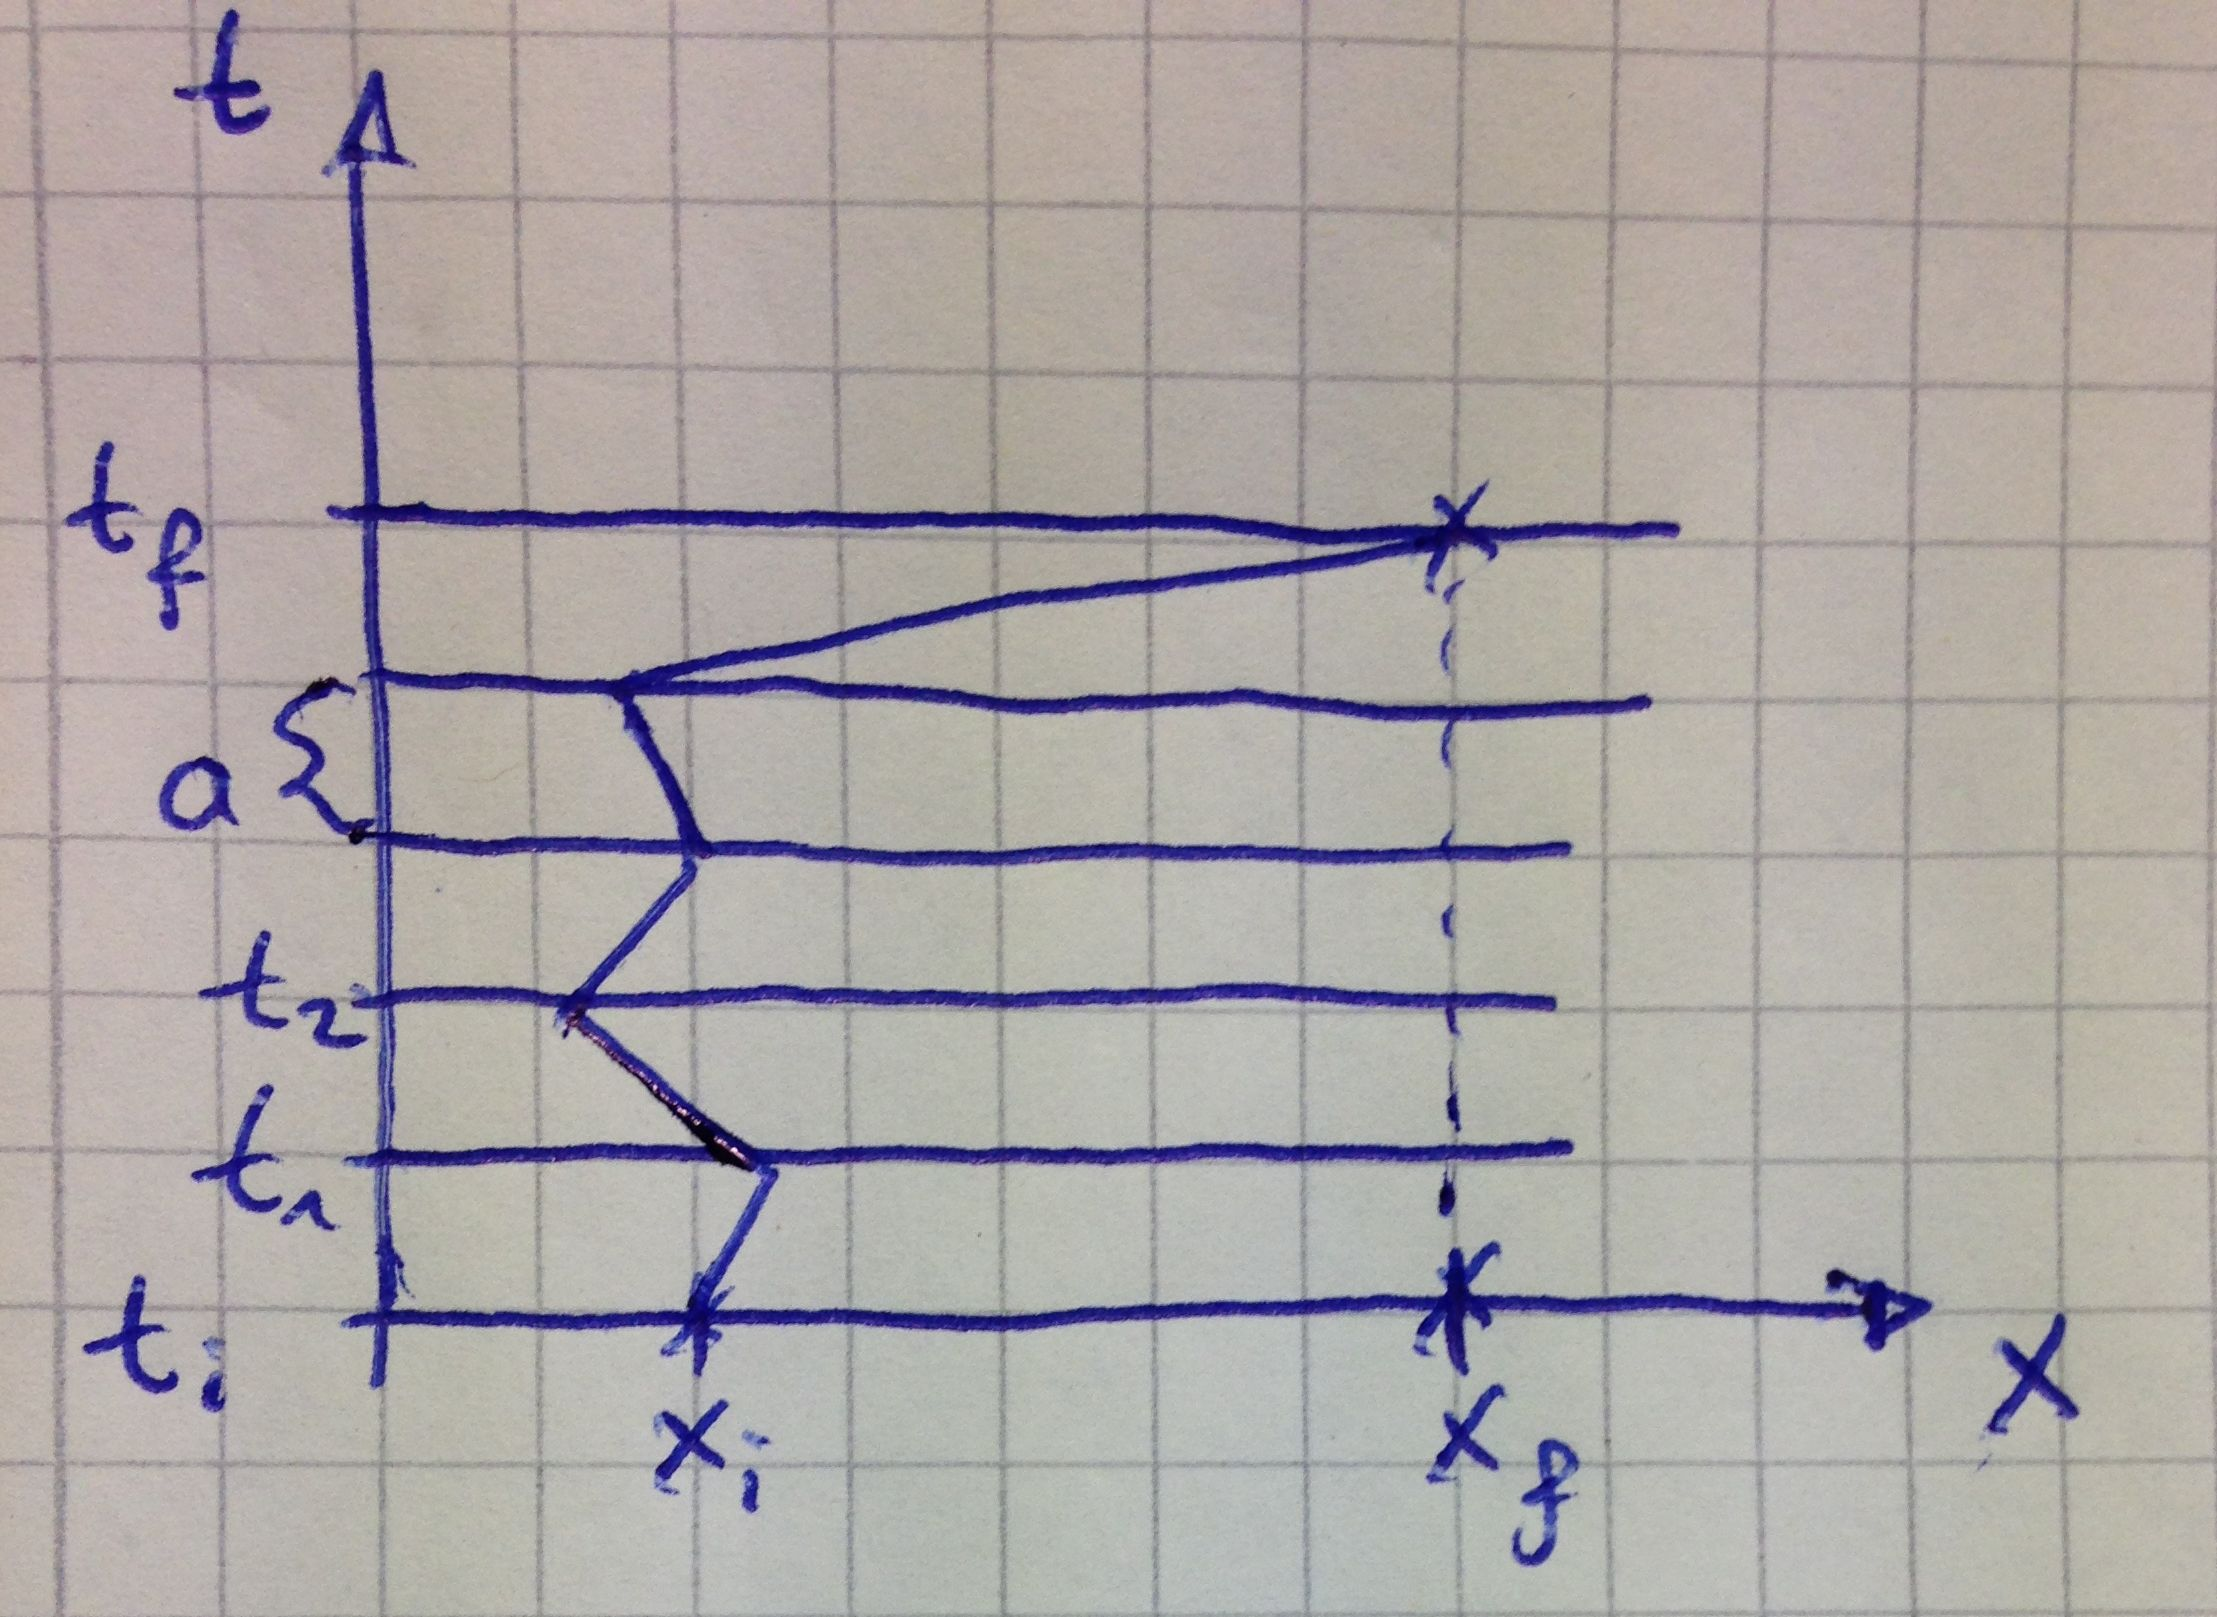
\includegraphics[width=10cm]{Uebergangsamplituden2}
	%	\end{center}
	%	\end{figure*} bild4
	\begin{align*}
		\int_{c_a} \diff \vec{r} \cdot \vec{A}(\vec{r}) - \int_{c_c} \diff \vec{r} \cdot \vec{A}(\vec{r}) &=
		\int_{c^{(1)}} \diff \vec{r} \cdot \vec{A}(\vec{r}) - \int_{c^{(2)}} \diff \vec{r} \cdot \vec{A}(\vec{r}) = \alpha_1 - \alpha_2 \\
		&= \oint_{\partial F_0} \diff \vec{f} \cdot \vec{A}(\vec{r}) 
		\overset{Stokes}{=} \int_{F_0} \diff \vec{f} \cdot \vec{B}(\vec{r}) = \Phi_m
	\end{align*}
	\begin{empheq}[box=\boxed]{align*}
		\Phi_m = \alpha_1 - \alpha_2
	\end{empheq}
Übergangsamplitude
	\begin{align*}
		{}_H \braket{\vec{x}; t_1 | \vec{y}; t_0}_H &= 
		\int [\diff^3 r] e^{i \frac{S[\vec{r}(t)]}{\hbar}} \\
		&\approx \int^{(1)} [\diff^3 r] e^{i \frac{S[\vec{r}(t)]}{\hbar}} 
		+ \int^{(2)} [\diff^3 r] e^{i \frac{S[\vec{r}(t)]}{\hbar}} 
	\end{align*}
	\begin{align*}
		\int^{(1)} [\diff^3 r] e^{\frac{i}{\hbar} S} &=
		\int^{(1)} [\diff^3 r] e^{\frac{i}{\hbar} S_0} e^{\frac{i}{\hbar} \int \diff \vec{r} \frac{q}{c} \vec{A}} 
		= \int^{(1)} [\diff^3 r] e^{\frac{i}{\hbar} S_0} e^{\frac{iq}{\hbar c} \alpha_1}  
		= K_1 e^{\frac{iq}{\hbar c} \alpha_1}\\
		\int^{(2)} [\diff^3 r] e^{\frac{i}{\hbar} S} &=
		\int^{(2)} [\diff^3 r] e^{\frac{i}{\hbar} S_0} e^{\frac{i}{\hbar} \int \diff \vec{r} \frac{q}{c} \vec{A}} 
		= \int^{(2)} [\diff^3 r] e^{\frac{i}{\hbar} S_0} e^{\frac{iq}{\hbar c} \alpha_2}
		=K_2 e^{\frac{iq}{\hbar c} \alpha_2}
	\end{align*}
	\begin{align*}
		\braket{\vec{x}; t_1| \vec{y}; t_0} &= 
		K_1 e^{\frac{iq}{\hbar c} \alpha_1} + K_2 e^{\frac{iq}{\hbar c} \alpha_2} + \ldots 
		\approx e^{\frac{iq}{\hbar c} \alpha_1} (K_1 + K_2 e^{\frac{iq}{\hbar c} (\alpha_2 -\alpha_1)})
	\end{align*}
Übergangswahrscheinlichkeitsdichte:
	\begin{align*}
		|\braket{\vec{x}; t_1 | \vec{y} , t_0}|^2 &=
		| K_1 + K_2 e^{-\frac{iq}{\hbar c} \Phi_m}|^2
	\end{align*}
hängt ab von magnetischem Fluss, obwohl Pfade (fast) nie durch Region mit $\vec{B}\neq \vec{0}$ laufen.

Korrekte Lösung:
	\begin{align*}
		|\braket{\vec{x}; t_1 | \vec{y} , t_0}|^2 &=
		\left|
			\sum_{n\in\mathds{Z}} K_{n+1} e^{in \frac{q}{\hbar c} \Phi_m}
		\right|^2
	\end{align*}
$n$ ist Windungszahl.
	\begin{align*}
		\Phi_m &= \frac{\hbar c}{q} 2\pi \cdot \ell ,& \ell&\in \mathds{Z} \\
	\end{align*}
$\Rightarrow$ Magnetfeld hat keinen Einfluss.

Ansonsten beeinflusst $\vec{B}$ das Interferenzmuster. 
\\
NB: Flussquantisierung in Supraleitern (London 1948)
	\subsection{Das euklidische Pfadintegral} (5.4)
	\begin{align*}
		S= \int_{-\infty}^{\infty} \diff t ~L(\vec{r}, \dot{\vec{r}})
	\end{align*}
			\begin{figure*} [h]
			\begin{center}
				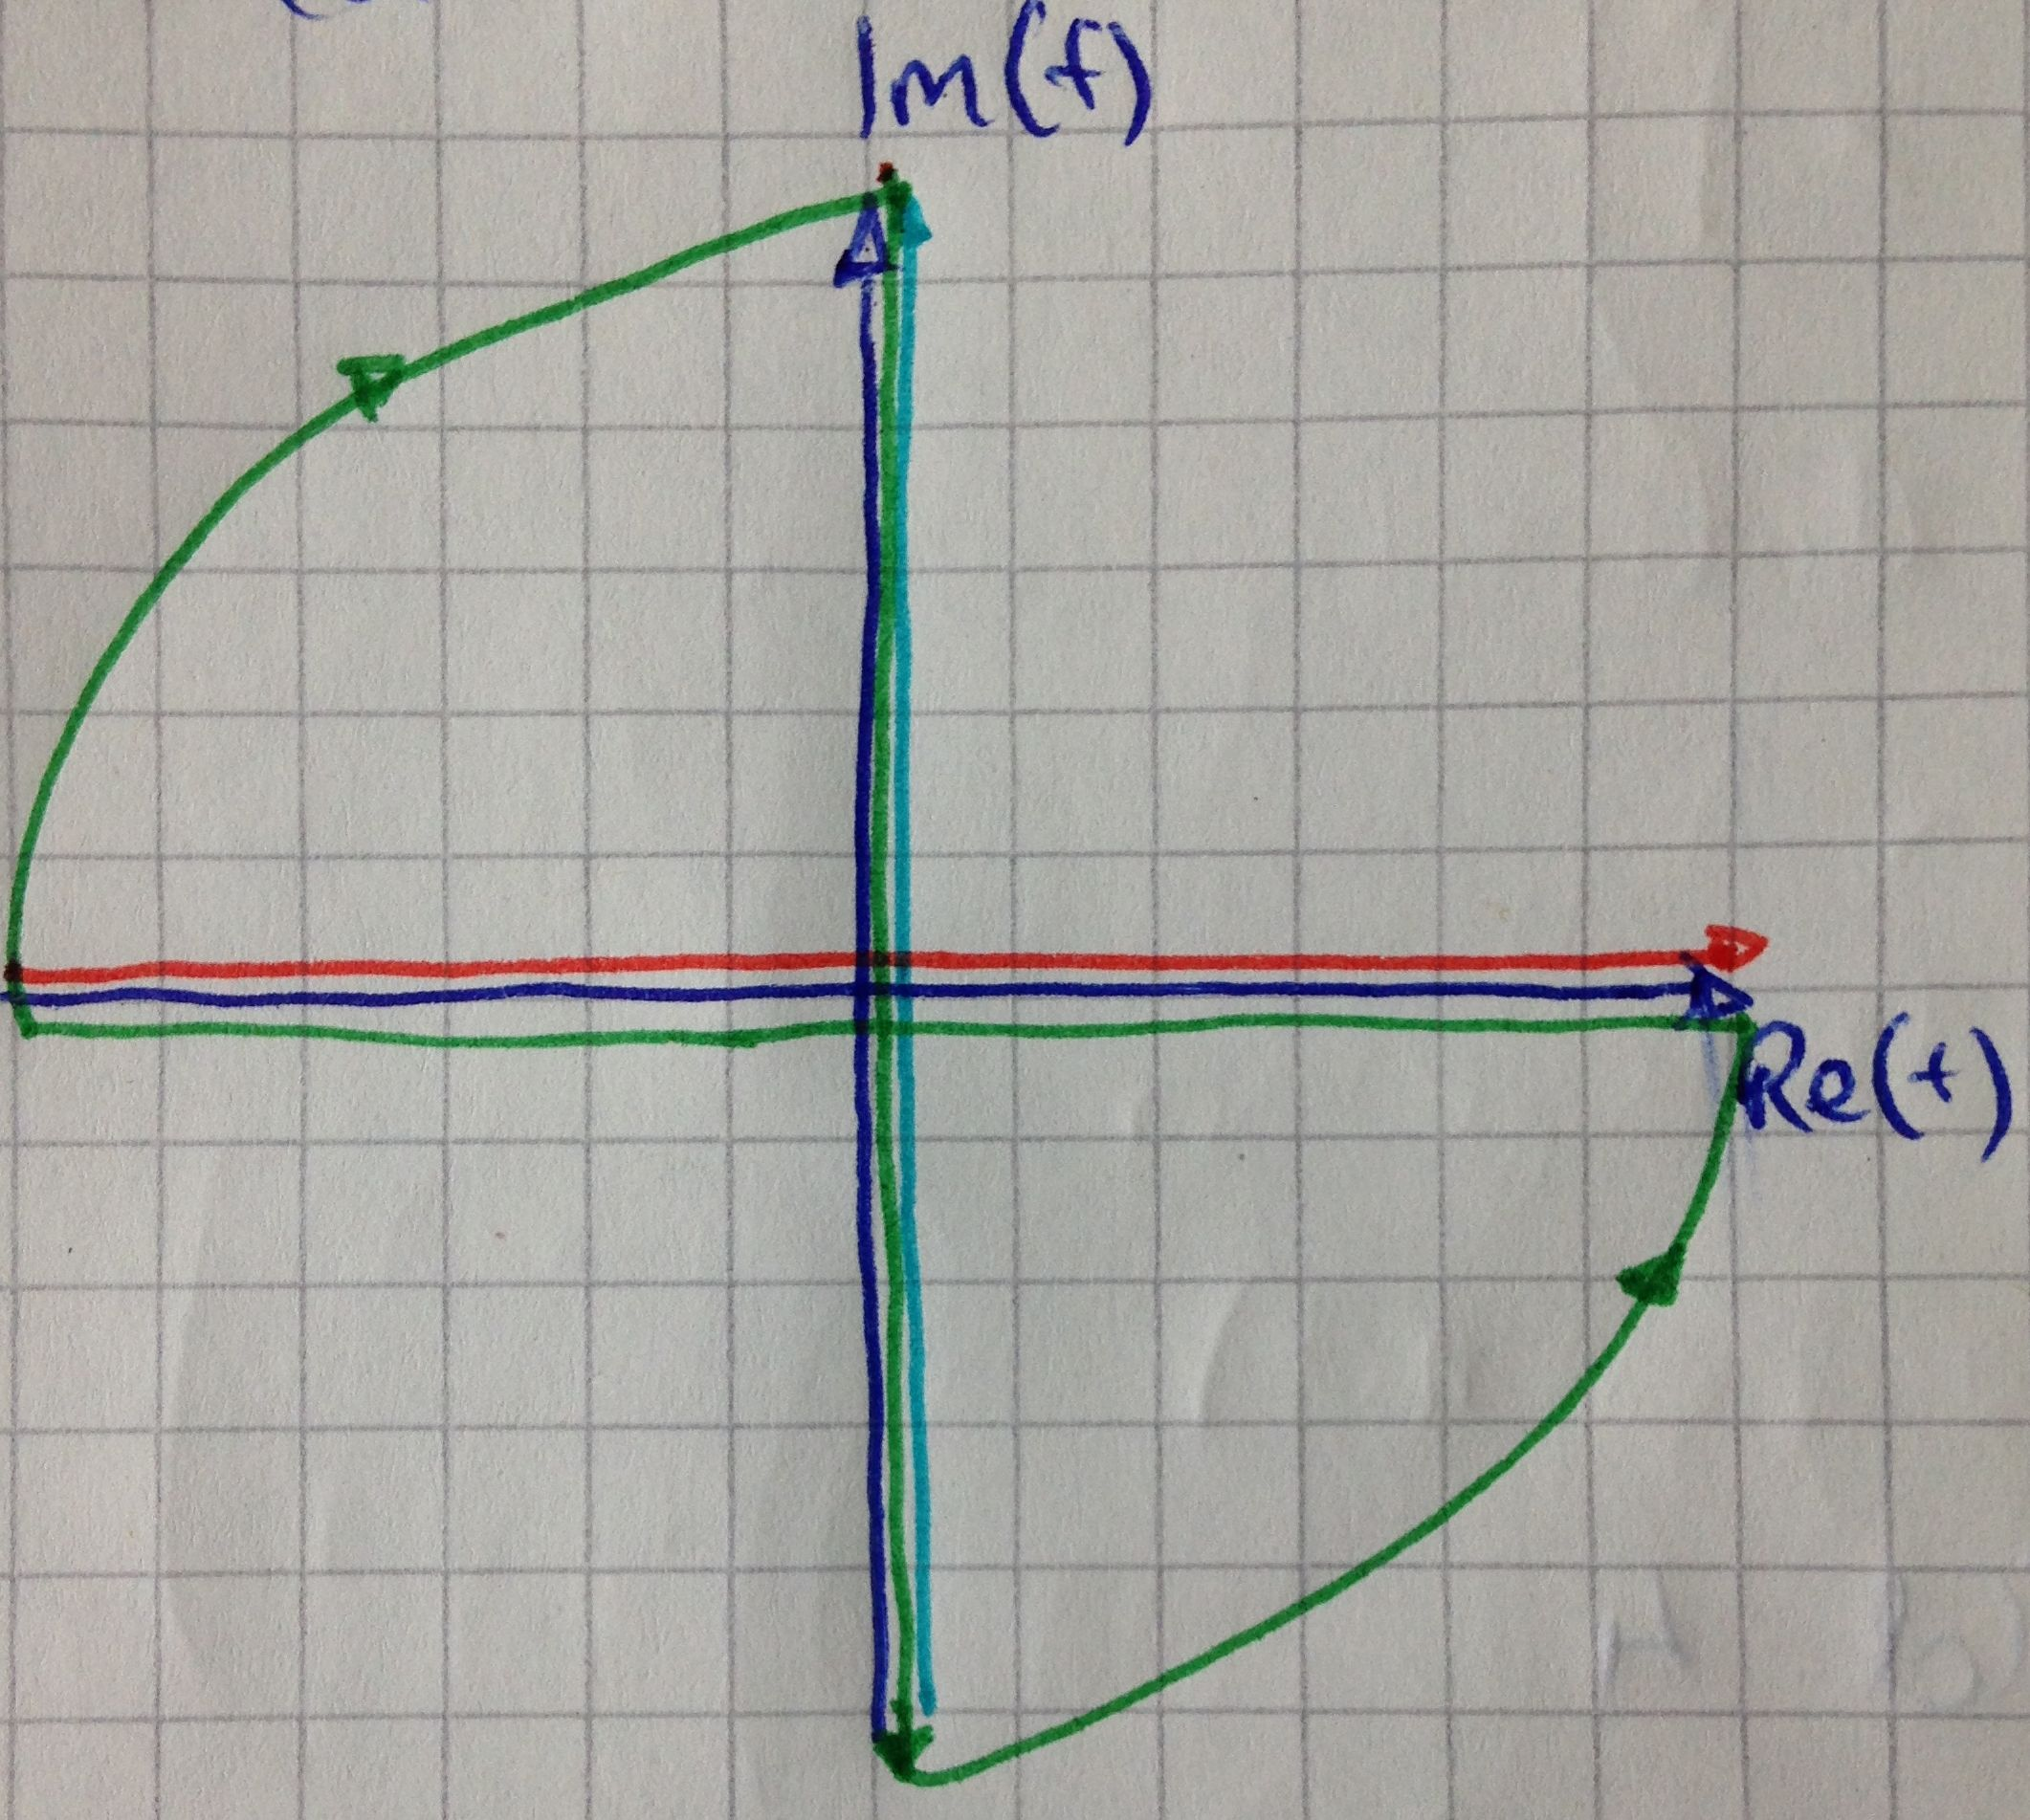
\includegraphics[width=10cm]{euklidisches_Pfradintegral1}
			\end{center}
			\end{figure*} 
\FloatBarrier
Annahmen:
	\begin{enumerate}[(1)]
		\item Kein Pol in 2. und 4. Quadranten
		\item $\int_{\text{untere grüne Kurve}} \diff t~L = \int_{\text{obere grüne Kurve}} \diff t ~L = 0$
	\end{enumerate}
	\begin{align*}
	\Rightarrow \int_{\text{über ganze grüne Kurve}} \diff t ~L = 0 = \int_{-\infty}^{\infty} \diff t ~L + \int_{i\infty}^{-i\infty} \diff t ~L
	\end{align*}	
	\begin{align*}
		S &= \int \limits_{-\infty}^{\infty} \diff t ~L = \int \limits_{-i\infty}^{i\infty} \diff t ~L = i \int \limits_{-\infty}^{\infty} \diff \tau \cdot L \\
		\tau &= + it \\
		e{\frac{i}{\hbar} S} &= e^{\frac{\int_{-\infty}^{\infty}\diff \tau ~L}{\hbar}} =
		\exp\left(-\frac{1}{\hbar} \int_{-\infty}^{\infty} \diff \tau ~L_E(\vec{r}, \frac{\partial \vec{r}}{\partial \tau})\right)
	\end{align*}
mit $\tau = i t$ Euklidische Zeit \\
$L_E = -L$: Euklidische Lagrangefunktion
	\begin{align*}
		\frac{\partial}{\partial t} &= i \frac{\partial}{\partial \tau} \\
		\frac{1}{2} m \left(\frac{\diff \vec{r}}{\diff t}\right)^2 &=
		-\frac{1}{2} m \left(\frac{\diff \vec{r}}{\diff \tau}\right)^2 \\
		L_E &= - L = \frac{1}{2} m \left(\frac{\diff \vec{r}}{\diff \tau}\right)^2 + V(\vec{r})
	\end{align*}
Euklidische Wirkung:
	\begin{align*}
		S_E &= \int_{-\infty}^{\infty} \diff \tau ~L_E
	\end{align*}
	\begin{align*}
		{}_H\braket{x_f; \tau= \infty | x_i ; \tau= -\infty}_H &= 
		\int [\diff x] e^{-\frac{S_E[x(t)]}{\hbar}}
	\end{align*}
$\tau$ ist keine ``echte'' Zeit mehr.\\

	\begin{tabular}{l l}
		Vorteil: & Keine komplexen Phasen. Nicht-klassische Pfade werden exponentiell \\
		 & mit $e^{-\frac{S_E}{\hbar}}$ unterdrückt.\\
		 Nachteil: & Wir haben Information über zeitliche Entwicklung verloren. \\
		 NB: & Pfadintegrale lassen sich auch in euklidischer Raumzeit herleiten:\\
		 & Transferoperator: 
		 $T_E = \exp\left(-\frac{a}{2\hbar} V(\hat{x})\right) \exp\left(-\frac{a}{\hbar} \frac{\hat{p}^2}{2m}\right) \exp\left(-\frac{a}{2\hbar} V(\hat{x})\right)$\\
		 Vorteil 2: & $\int [\diff x] e^{-\frac{S[x(t)]}{\hbar}}$ lässt sich als relative Wahrscheinlichkeit (Maß) interpretieren
	\end{tabular}
	\subsection{2-Punkt Funktion}
	\begin{align*}
		G^{(2)} (\tau_2, \tau_1) &=
		\frac{{}_H\braket{x_f; \tau_f = \infty | \hat{x} (\tau_2) \hat{x}(\tau_1) | x_i; \tau_i = \infty}_H}{{}_H\braket{x_f | x_i}_H} \\
		\text{Enwickle nach Eigenzuständen von }H& \\
		&= \sum_{m, n} \frac{\braket{x_f | e^{-\hat{H} \tau_f} | m} 
		\braket{m | \hat{x} (\tau_2) \hat{x} (\tau_1)| n} \braket{n | e^{\hat{H} \tau_i} | x_i}}{\sum_n \braket{x_f | e^{-\hat{H}\tau_f} | n} \braket{n | e^{\hat{H} \tau_i} | x_i}} \\
		&= \frac{\sum_{m,n} e^{-E_m\tau_f}e^{E_n\tau_i} \braket{x_f | m} \braket{n|x_i} \braket{m | \hat{x} (\tau_2) \hat{x} (\tau_1) | n}}{\sum_n e^{-E_n(\tau_f -\tau_i)} \braket{x_f | n} \braket{x_i | m}}\\
		&\overset{\tau_f \rightarrow \infty,~\tau_i \rightarrow \infty}{\longrightarrow}
		\frac{\braket{x_f | 0} \braket{0 | x_i}}{\braket{x_f | 0} \braket{0 | x_i}} \braket{m | \hat{x} (\tau_2) \hat{x} (\tau_1) | n}
	\end{align*}
Trick: Kompaktifiziere Zeit:
	\begin{align*}
		\tau_i &= 0,& \tau_f&= \tau & &\circlearrowright \\
		x(0) &= x(\tau) = x(\tau_i) = x(\tau_f) = x_i = x_f
	\end{align*}
	\begin{align*}
		\sum_x \braket{x | x} &= 
		\sum_x \braket{x | \hat{\mathrm{T}}_E^n | x} = \mathrm{Sp} \hat{\mathrm{T}_E^n} \\
		&\overset{n \rightarrow \infty}{=} \mathrm{Sp} e^{-H\tau} = Z_E = 
		\int \diff x_0 \ldots \diff x_{n-1} e^{-S_E[x]}
	\end{align*}
$[x]$ periodische Pfade in $\tau$.  $x_f$, $x_i$ nicht fest
	\begin{align*}
		G^{(2)}(\tau_2, \tau_1) &=
		\frac{\int \diff x \braket{x | x(\tau_2) x(\tau_1) | x}}{\int \diff x\braket{x | x}} 
		= \braket{0 | x(\tau_2) x(\tau_1) | 0} 
		& \tau_2 &> \tau_1 \\
		&= \sum_n \braket{0 | e^{H \tau_2} \hat{x} (0) e^{-H \tau_2} | n}
		\braket{n | e^{H \tau_1} \hat{x} (0) e^{-H \tau_1} | 0} \\
		&= \sum_n e^{E_0(\tau_2 - \tau_1)} e^{-E_n(\tau_2 - \tau_1)}
		\braket{0 | \hat{x} (0) | n} \braket{n | \hat{x} (0) | 0} \\
		&\overset{E_0 = 0}{=} |\braket{0 | \hat{x} | 0 }|^2 + e^{-E_1(\tau_2 - \tau_1)} 
		|\braket{0 | \hat{x} | 1}|^2 + \ldots
	\end{align*}
$E_1$ Abfall der 2-Punkt funktion mit euklidischer Zeit ergibt Spektrum von $H [(E_0), E_1 ,E_2, \ldots]$

Wie berechne ich $G^{(2)}$? 
	\begin{align*}
		G^{(2)} (\tau_2, \tau_1) &\coloneqq 
		\braket{0 | \mathrm{T} \hat{x}(\tau_2) \hat{x}(\tau_1) | 0} \\ 
		&= \frac{\int [\diff x] e^{-S_E[x]} x(\tau_2) x(\tau_1)}{Z_E}
	\end{align*}
Hier ist kein T (Zeitordnung) notwendig, kein ``1''. Zahlen, keine Operatoren. 

	\subsection{Erzeugende Funktionale}
$n$-Punkt Funktionen $\Rightarrow$ Alle Observablen \\
Erzeugendes Funktional bekannt $\Rightarrow$ alle $n$-Punkt-Funktionen sind berechenbar.
	\begin{align*}
		Z_E [j] &= \frac{\int [\diff x] e^{-S_E + \int \diff \tau j(\tau) x(\tau)}}{\int[\diff x] e^{-S_E}}
		&\Rightarrow Z_E[0] &= 1 \neq Z_E (\text{weil unten ja }Z_E) 
	\end{align*}
$j = j(\tau)$

Funktionalableitung
	\begin{align*}
		\left.\frac{\delta Z_E(j)}{\delta j(\tau_1)} \right|_{j = 0} 
		&= \frac{\int [\diff x] e^{-S_E}x(\tau_1)}{Z_E} 
		= \braket{0 | \hat{x} (\tau_1) | 0} \\
		\left.\frac{\delta Z_E(j)}{\delta j (\tau_1) \delta j(\tau_2)} \right|_{j = 0}
		&= \frac{\int [\diff x] e^{-S_E[x]} x(\tau_2) x(\tau_1)}{Z_E}
		= \braket{0 | \mathrm{T} \hat{x} (\tau_2) \hat{x}(\tau_1) | 0} 
	\end{align*}
	\begin{align*}
		&\Rightarrow \braket{0 | \mathrm{T} x(\tau_1) \ldots x(\tau_N) | 0} = 
		\left.\frac{\delta^N Z[j]}{\delta j(\tau_1) \ldots \delta j(\tau_N)} \right|_{j= 0} \\
		&\Rightarrow \text{Alle }n\text{-Punktfunktionen lassen sich aus }Z_E[j]\text{ berechnen!}
	\end{align*}
Taylorentwicklung 
	\begin{align*}
		Z_E[j] &= \sum_{k = 0}^{\infty} \frac{1}{k!} 
		\int \diff \tau_1 \diff \tau_2 \ldots \diff \tau_k 
		j(\tau_1) j(\tau_2) \ldots j(\tau_k) 
		\frac{\delta^k Z_E [j]}{\delta j(\tau_1) \cdots \delta j(\tau_k)} \\
		&= \sum_{k = 0}^{\infty} \frac{1}{k!}
		\int \diff \tau_1 \ldots \diff \tau_k j(\tau_1) \ldots j(\tau_k) 
		\braket{0 | \mathrm{T} \hat{x} (\tau_1) \ldots \hat{x} (\tau_k) | 0} \\
		&= \braket{0 | \mathrm{T} \exp \left[\int \diff \tau j (\tau) \hat{x}(\tau)\right] | 0} \\
		&= \frac{1}{Z_E} \int [\diff x] e^{-S_E} e^{\int \diff \tau j(\tau) x(\tau)}
	\end{align*}	
	

	\subsection{Beispiel: Harmonischer Oszillator}
	\begin{align*}
		S_E &= \int \diff \tau \left(\frac{m}{2} \dot{x}^2 + \frac{1}{2} m \omega^2 x^2\right)
		& &\dot{x}^2 = \left(\frac{\diff}{\diff \tau} x \right)^2\\
		&= \frac{m}{2} \int_{-\infty}^\infty \diff \tau ~x(\tau) \left(- \frac{\diff^2}{\diff \tau^2} + \omega^2\right) x(\tau) \\
		S_E [x, j] &= \frac{m}{2} \int_{-\infty}^\infty \diff \tau ~x(\tau)
		\left(- \frac{\diff^2}{\diff \tau^2} + \omega^2\right) x(\tau)
		- \int_{-\infty}^\infty \diff \tau j(\tau) x(\tau)
	\end{align*}
Berechne 
	\begin{align*}
		Z_E [j] = \frac{\int [\diff x] e^{-S_E[x, j]}}{Z_E} 
	\end{align*}
2 Möglichkeiten der Berechnung	
	\begin{enumerate}[1)]
		\item Integral hat die Form
			\begin{align*}
				\int [\diff x] e^{-S_E[x, j]} \overset{n \rightarrow \infty}{=}
				\int \diff x_0 \ldots \diff x_{n - 1} 
				e^{-\frac{1}{2} x^T A x + b x} 
			\end{align*}
			mit $A= A^\dagger$, $x\in \mathds{R}^n$ 
		\item Entwickle um klassische Lösung \marginpar{keine Ahnung wann dieser Punkt vorbei war}
			\begin{align*}
				0 &= \frac{\delta S_E[x, j]}{\delta x(\tau)} =
				m \left(- \frac{\diff^2}{\diff \tau^2} + \omega^2\right) x(\tau) - j(\tau)
			\end{align*}
			Randbedingung $x(\tau) \rightarrow 0$ für $\tau \rightarrow \pm \infty$
			\begin{align*}
				A &= - \frac{\diff^2}{\diff \tau^2} + \omega^2 \\
				Ax &= \frac{j}{m} ~(\text{Bewegungsgleichung}) 
				& \int \diff \tau' A(\tau, \tau') x(\tau') &= \frac{1}{m} j(\tau) \\
				x &= \frac{1}{m} A^{-1} j
			\end{align*}
			Konvention: $D_E = -A^{-1} = ?$
			\begin{align*}
				x(\tau) &= \int\limits_{-\infty}^{\infty} \frac{\diff \Omega}{2 \pi} e^{-i\Omega \tau} \tilde{x}(\Omega) ,&
				j(\tau) &= \int\limits_{-\infty}^{\infty} \frac{\diff \Omega}{2 \pi} e^{-i\Omega \tau} \tilde{j}(\Omega)
			\end{align*}
			\begin{align*}
				&\Rightarrow (\Omega^2 + \omega^2) \tilde{x}(\Omega) = \frac{1}{m} \tilde{j}(\Omega) &
				\Rightarrow \tilde{x}(\Omega) &= \frac{1}{m} \frac{\tilde{j}(\Omega)}{\Omega^2 + \omega^2} \\
				x(\tau) &= \int\limits_{-\infty}^{\infty} \frac{\diff \Omega}{2 \pi}
				\frac{1}{m} \frac{1}{\Omega^2 + \omega^2} e^{-i\Omega \tau} 
				\int \diff \tau' e^{i\Omega \tau'} j(\tau') \\
				&= -\frac{1}{m} \int \diff \tau' D_E(\tau - \tau') j(\tau') &
				\text{mit }D_E(\tau, \tau') &= - \int \frac{\diff \Omega}{2 \pi} \frac{e^{-i \Omega (\tau-\tau')}}{\Omega^2 + \omega^2}
			\end{align*}
			\begin{align*}
				x &= \frac{1}{m} A^{-1} j = - \frac{1}{m} D_E j \\
				D_E (\tau) &= \int \frac{\diff \Omega}{2 \pi} \frac{e^{-\Omega \tau}}{(\Omega^2 + \omega^2)(\Omega^2 - \omega^2)} \\
				&= \Theta(\tau) \frac{e^{-\omega \tau}}{2 \omega} 
				+ \Theta (-\tau) \frac{e^{-\omega \tau}}{2 \omega} = \frac{e^{-\omega|\tau|}}{2 \omega}
			\end{align*}
			$+$ für $\tau < 0$ und $-$ für $\tau > 0$
			\begin{align*}
				A D_E(\tau) &= -\delta(\tau) & 
				\text{bzw. } A \cdot D_E = - \mathds{1} 
			\end{align*}
			$D_E$ ist Green-Funktion für $A$
			\begin{align*}
				\boxed{D_E (\tau) = \frac{e^{-\omega|\tau|}}{2 \omega}}
			\end{align*}
			Pfad 
			\begin{align*}
				x(\tau) &= x_c(\tau) + y(\tau) ,& x_c(\tau) &= \left(-\frac{1}{m} D_E j\right) (\tau)
			\end{align*}
			\begin{align*}
				S_E[x, j] &= S_E [x_c ,j]
				+ \frac{m}{2} \int \diff \tau y (\tau) \left(-\frac{\diff^2}{\diff^2 \tau} + \omega^2\right)y(\tau) \\
				S_E[x , j] &= \frac{1}{2m} \int \diff \tau \diff \sigma 
				j(\tau) D_E (\tau - \sigma) j(\sigma) \\
				Z[j] Z_E &= \int [dx] e^{-\frac{m}{2} x^T A x + j^T x}  \\
				&= \int[\diff y] e^{-\frac{1}{2m} j^T D_E j} e^{-\frac{m}{2} y^T A y}
			\end{align*}
			\begin{align*}
				Z_E &= \int [\diff y] e^{-\frac{m}{2} y^T A y} \\
			\Rightarrow &
			\boxed{
					Z[j] = \exp \left(
						-\frac{1}{2 m} \int \diff \tau \diff \sigma j(\tau) D_E (\tau - \sigma) j(\sigma)
					\right)
				}
			\end{align*}
			weil Green-Integral
			\begin{align*}
			\braket{0 | \mathrm{T} \hat{x} (\tau_1) \hat{x}(\tau_2)| 0} &=
			\frac{\delta^2}{\delta j(\tau_1) \delta j(\tau_2)} \left.Z_E[x, j]\right|_{j = 0}\\
			&= -\frac{1}{m} D_E (\tau_1 - \tau_2) 
			\end{align*}
			2-Punkt Greenfunktion.. n-Punktfunktionen sind $\sim$ Greenfunktion
	\end{enumerate}
	\subsection{Systeme mit quadratischer Wirkung}
	\begin{align*}
		S_E &= \frac{1}{2} (x, Ax) \coloneqq
		\frac{1}{2} \int \diff \tau_1 \tau_2 x(\tau_1) A(\tau_1, \tau_2) x(\tau_2)
	\end{align*}
Beispiel: Harmonischer Oszillator
	\begin{align*}
		A &= m \left(-\frac{\diff^2}{\diff \tau^2} + \omega^2\right) \\
		\text{Kern von }A&:~ A(\tau_1, \tau_2) = m \left(-\frac{\diff^2}{\diff \tau^2} + \omega^2\right) \delta(\tau_1 - \tau_2) \\
		(j, x) &= \int \diff \tau j(\tau) x(\tau) 
	\end{align*}
``Zustandssumme'': 
	\begin{align*}
		Z_E &= \int [\diff x] e^{-\frac{1}{2} (x, Ax)} 
	\end{align*}
Erzeugendes Funktional
	\begin{align*}
		Z_E[j] &= \frac{1}{Z_E} \int [\diff x] e^{-\frac{1}{2} (x, Ax) + (j,x)} 
		&\Rightarrow Z_E[0] &= 1 
	\end{align*}
$Z_E$ lässt sich berechnen
	\begin{align*}
		\int \limits_{-\infty}^{\infty} \diff x e^{-\frac{a}{2} x^2 + bx} &=
		\sqrt{\frac{2 \pi}{a}} e^{\frac{b^2}{2a}} &
		a &> 0
	\end{align*}
Endlich dimensionaler Vektorraum:
	\begin{align*}
		A_{ij} , i,j &= 1, \ldots, n, A \text{ symmetrisch + positiv} \\
		\leadsto (x, Ax) &= \sum_{i,j} x_i A_{ij} x_j \\
		Z_E &= \int \diff^n x e^{-\frac{1}{2} (x, Ax)}
		= \int \diff^n x e^{-\frac{1}{2} \sum_{i = 1}^{n} \lambda_i x_i'^2}
		= \prod_{i = 1}^{n} \int \diff x' e^{-\frac{1}{2} \lambda_i x'^2} \\
		&= \frac{(\sqrt{2 \pi})^n}{\sqrt{\prod_i \lambda_i}} = 
		\left(\frac{(2 \pi)^n}{\det A}\right)^{\frac{1}{2}} \\
		Z_E [j] &= \frac{1}{Z_E} \int \diff^n x e^{-\frac{1}{2} (x, Ax) + (j,x)} 
		= e^{\frac{1}{2} (j, A^{-1} j)} \\
		\text{für } n= 1 &: e^{\frac{j_1^2}{e^{2A_{11}}}}
	\end{align*}
Pfadintegral mit $i \mapsto$ koninuierlicher ``Index'' $\tau_1$:
	\begin{align*}
		Z_E [j] &= \exp \left\{\frac{1}{2} (j, A^{-1}j)\right\} =
		\exp \left\{-\frac{1}{2}\int \diff \tau_1 \diff \tau_2  j(\tau_1) D_E (\tau_1, \tau_2) j(\tau_2)\right\} \\
		\text{mit } D_E &= A^{-1} \Rightarrow A D_E = - \mathds{1} \\
		\int \diff \tau' A(\tau_1, \tau') D_E (\tau', \tau_2) &= -\delta (\tau_1- \tau_2)
	\end{align*}
$D_E$ ist Greenfunktion von $A$
	\subsection{Tunneln durch eine Potentialbarriere}
	\begin{align*}
		V(x) = \lambda(x^2- a^2)^2
	\end{align*}
	\begin{figure}
		\begin{center}
			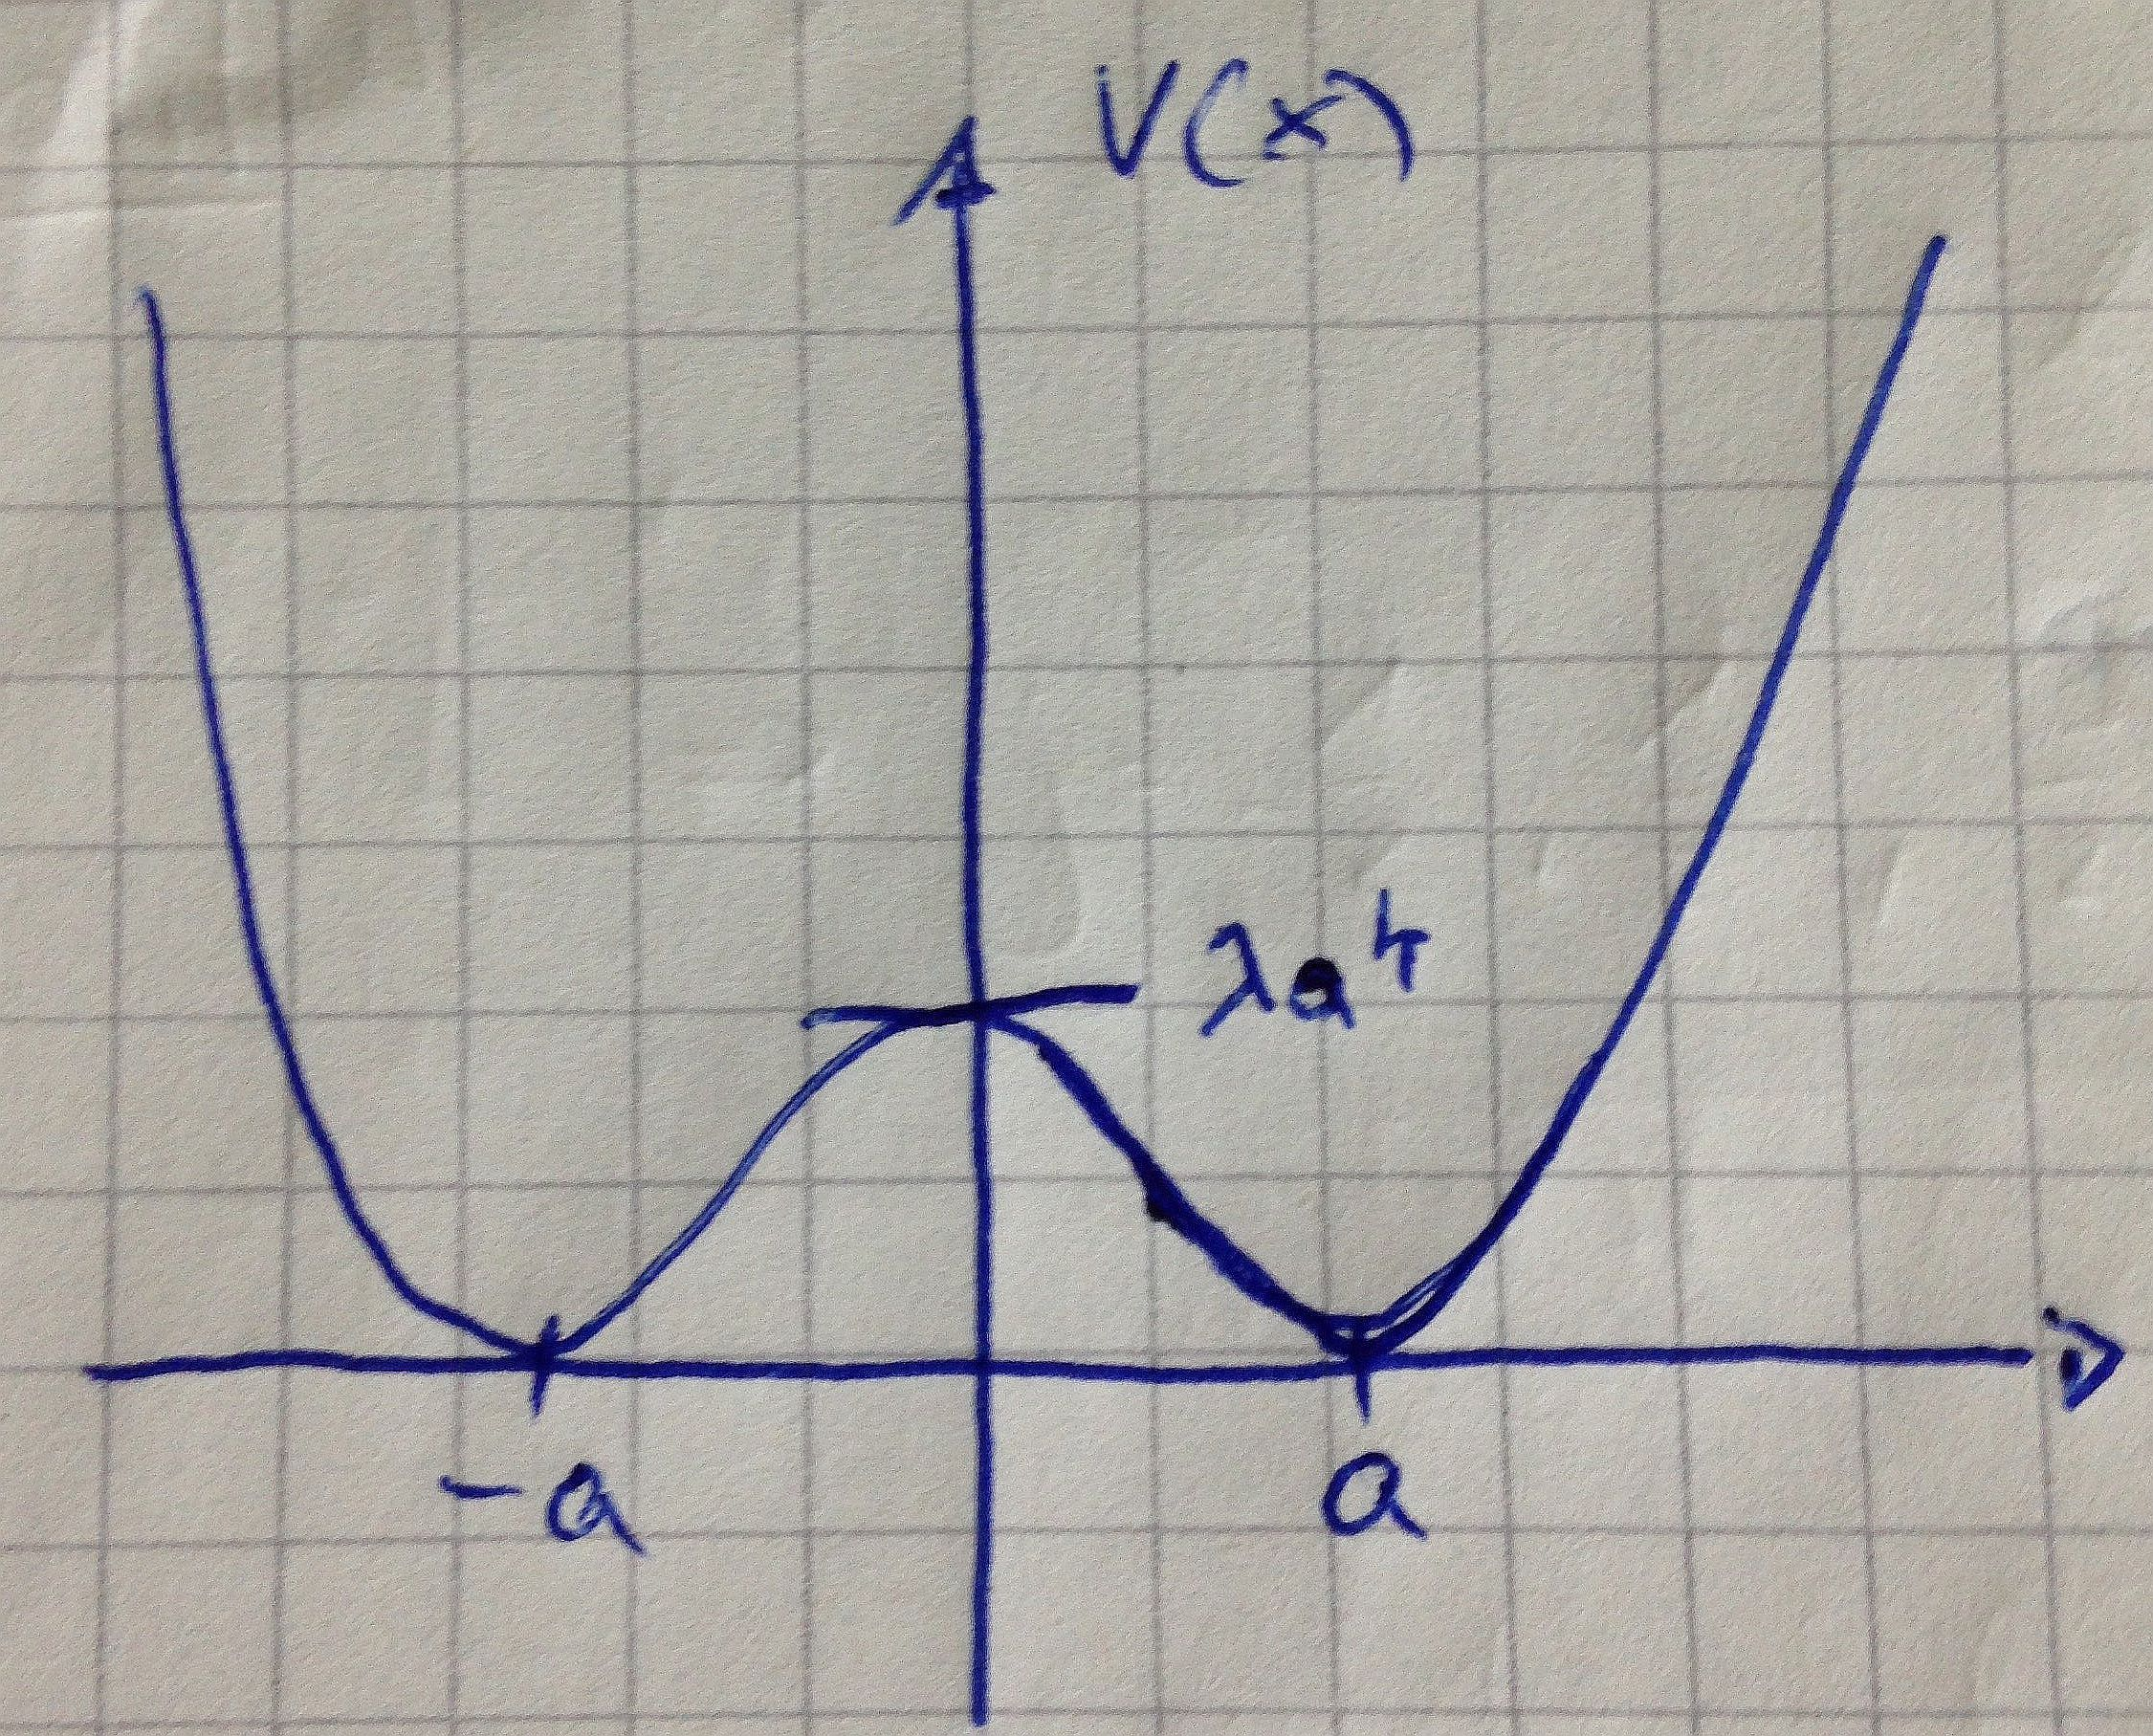
\includegraphics[width= 0.5\textwidth]{Tunneln_durch_eine_Potentialbarriere1}
		\end{center}
	\end{figure}
\FloatBarrier
Grundzustand $\ket{0}$ (symmetrische Wellenfunktion)
\FloatBarrier
	\begin{figure}[h]
		\begin{center}
			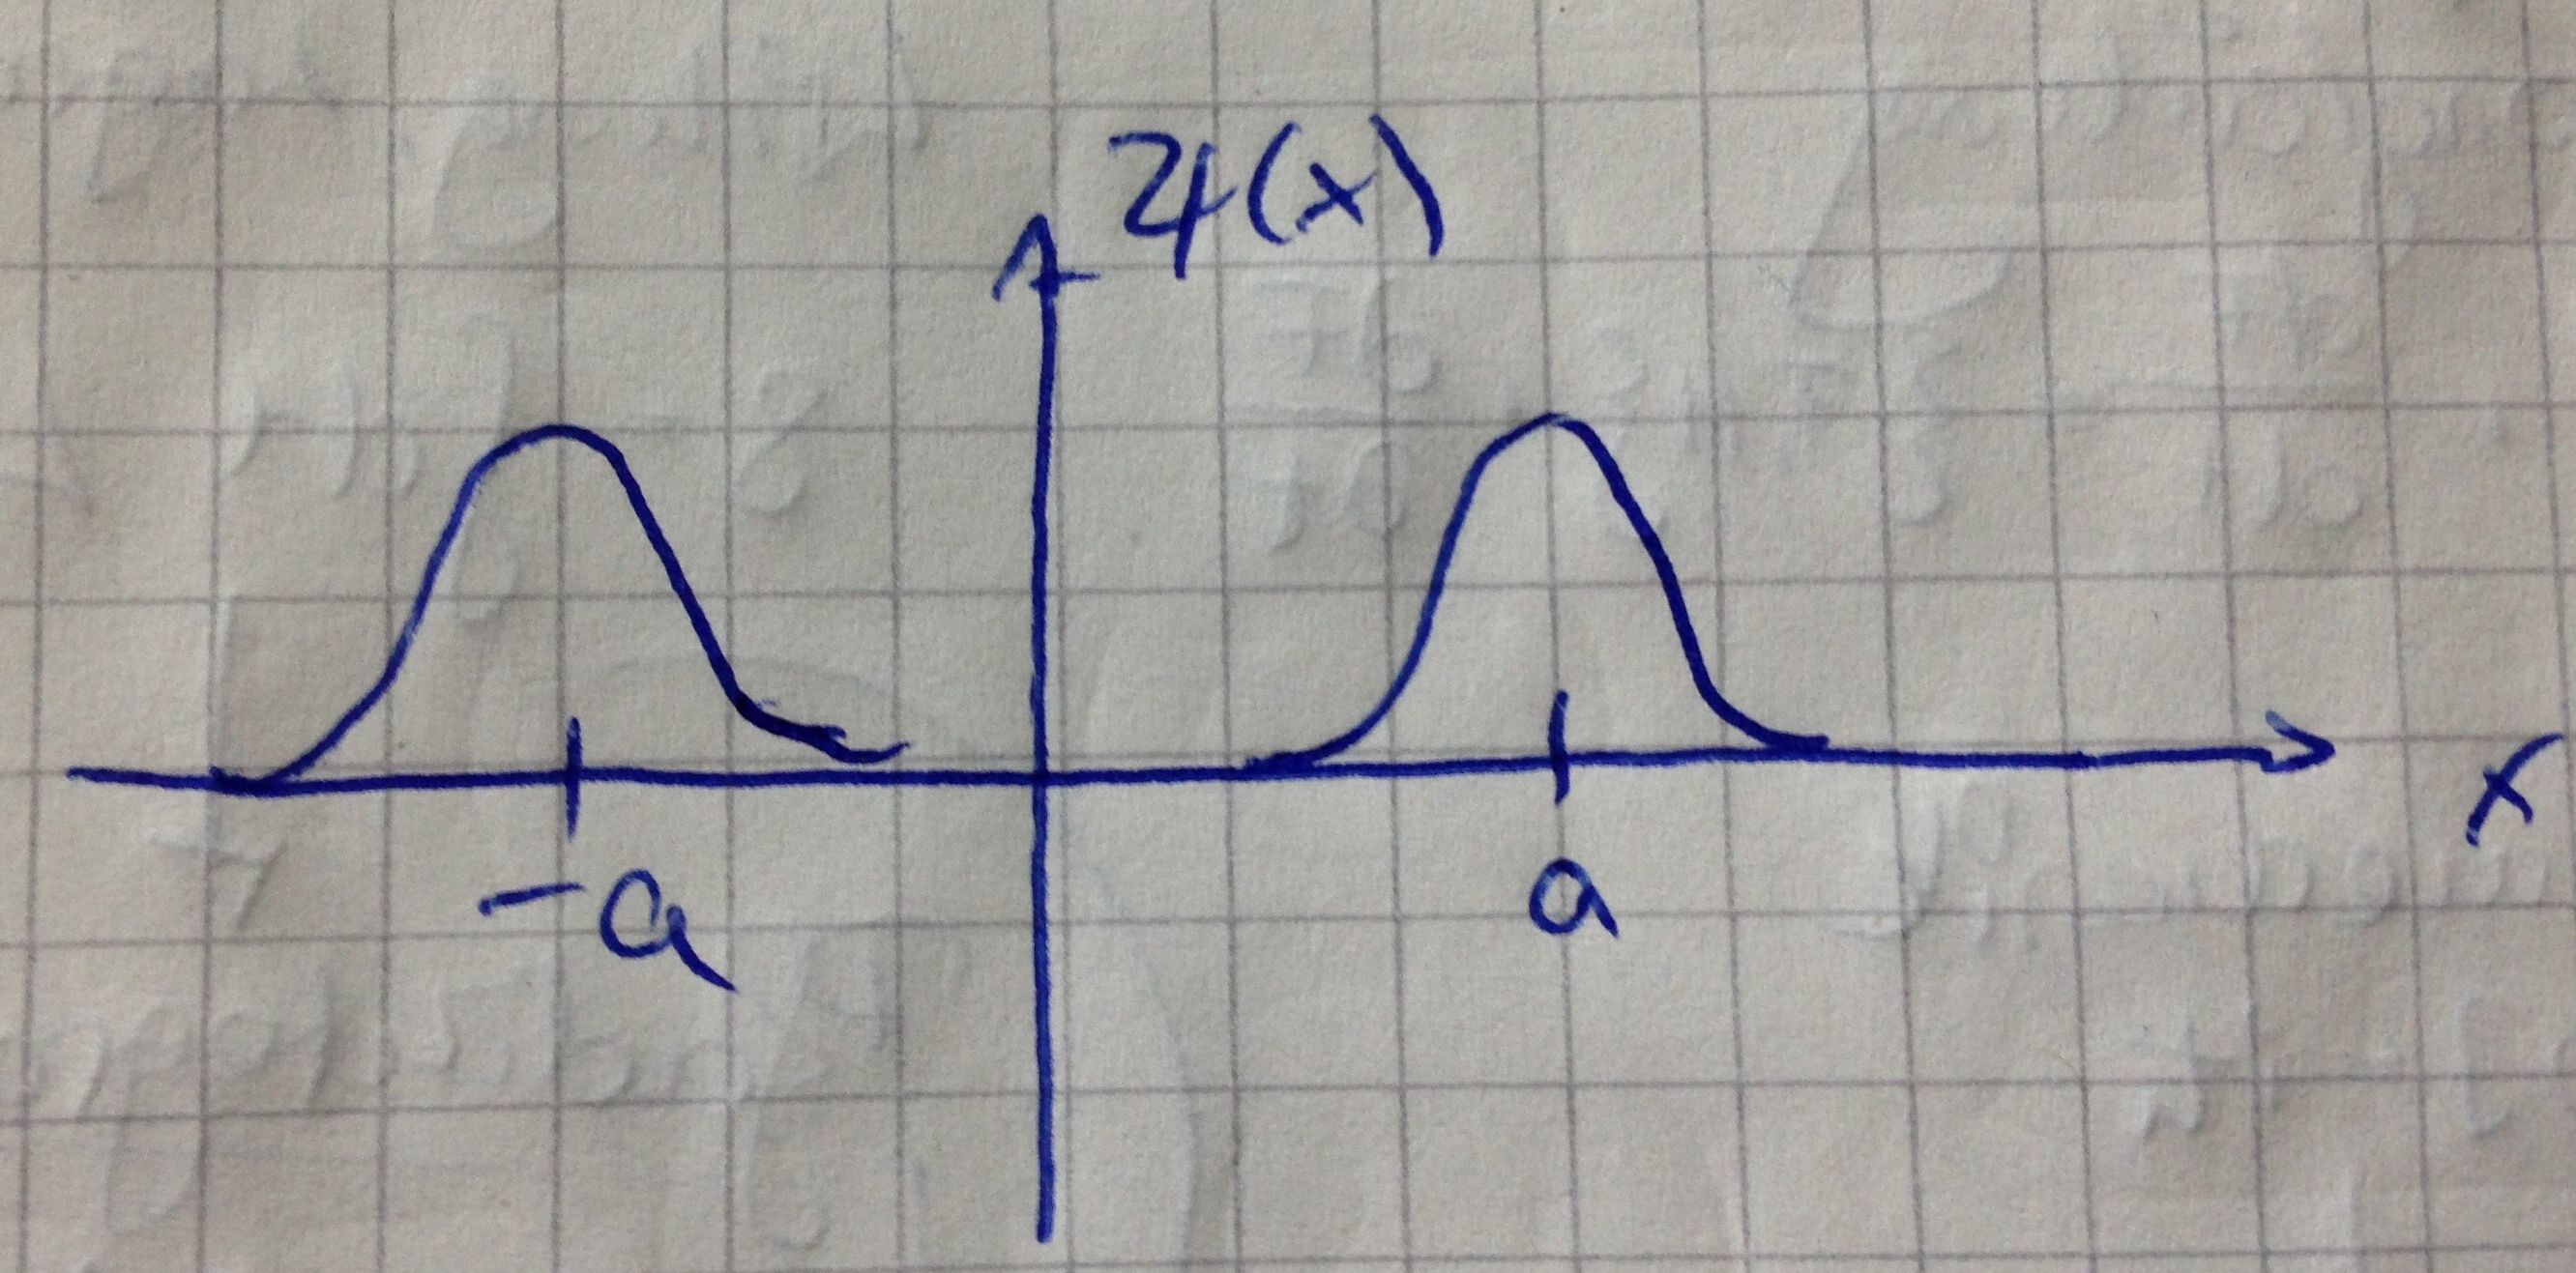
\includegraphics[width= 0.6\textwidth]{Tunneln_durch_eine_Potentialbarriere2}
		\end{center}
	\end{figure}
\newpage
1. Anregung $\ket{1}$
	\begin{figure} [h]
		\begin{center}
			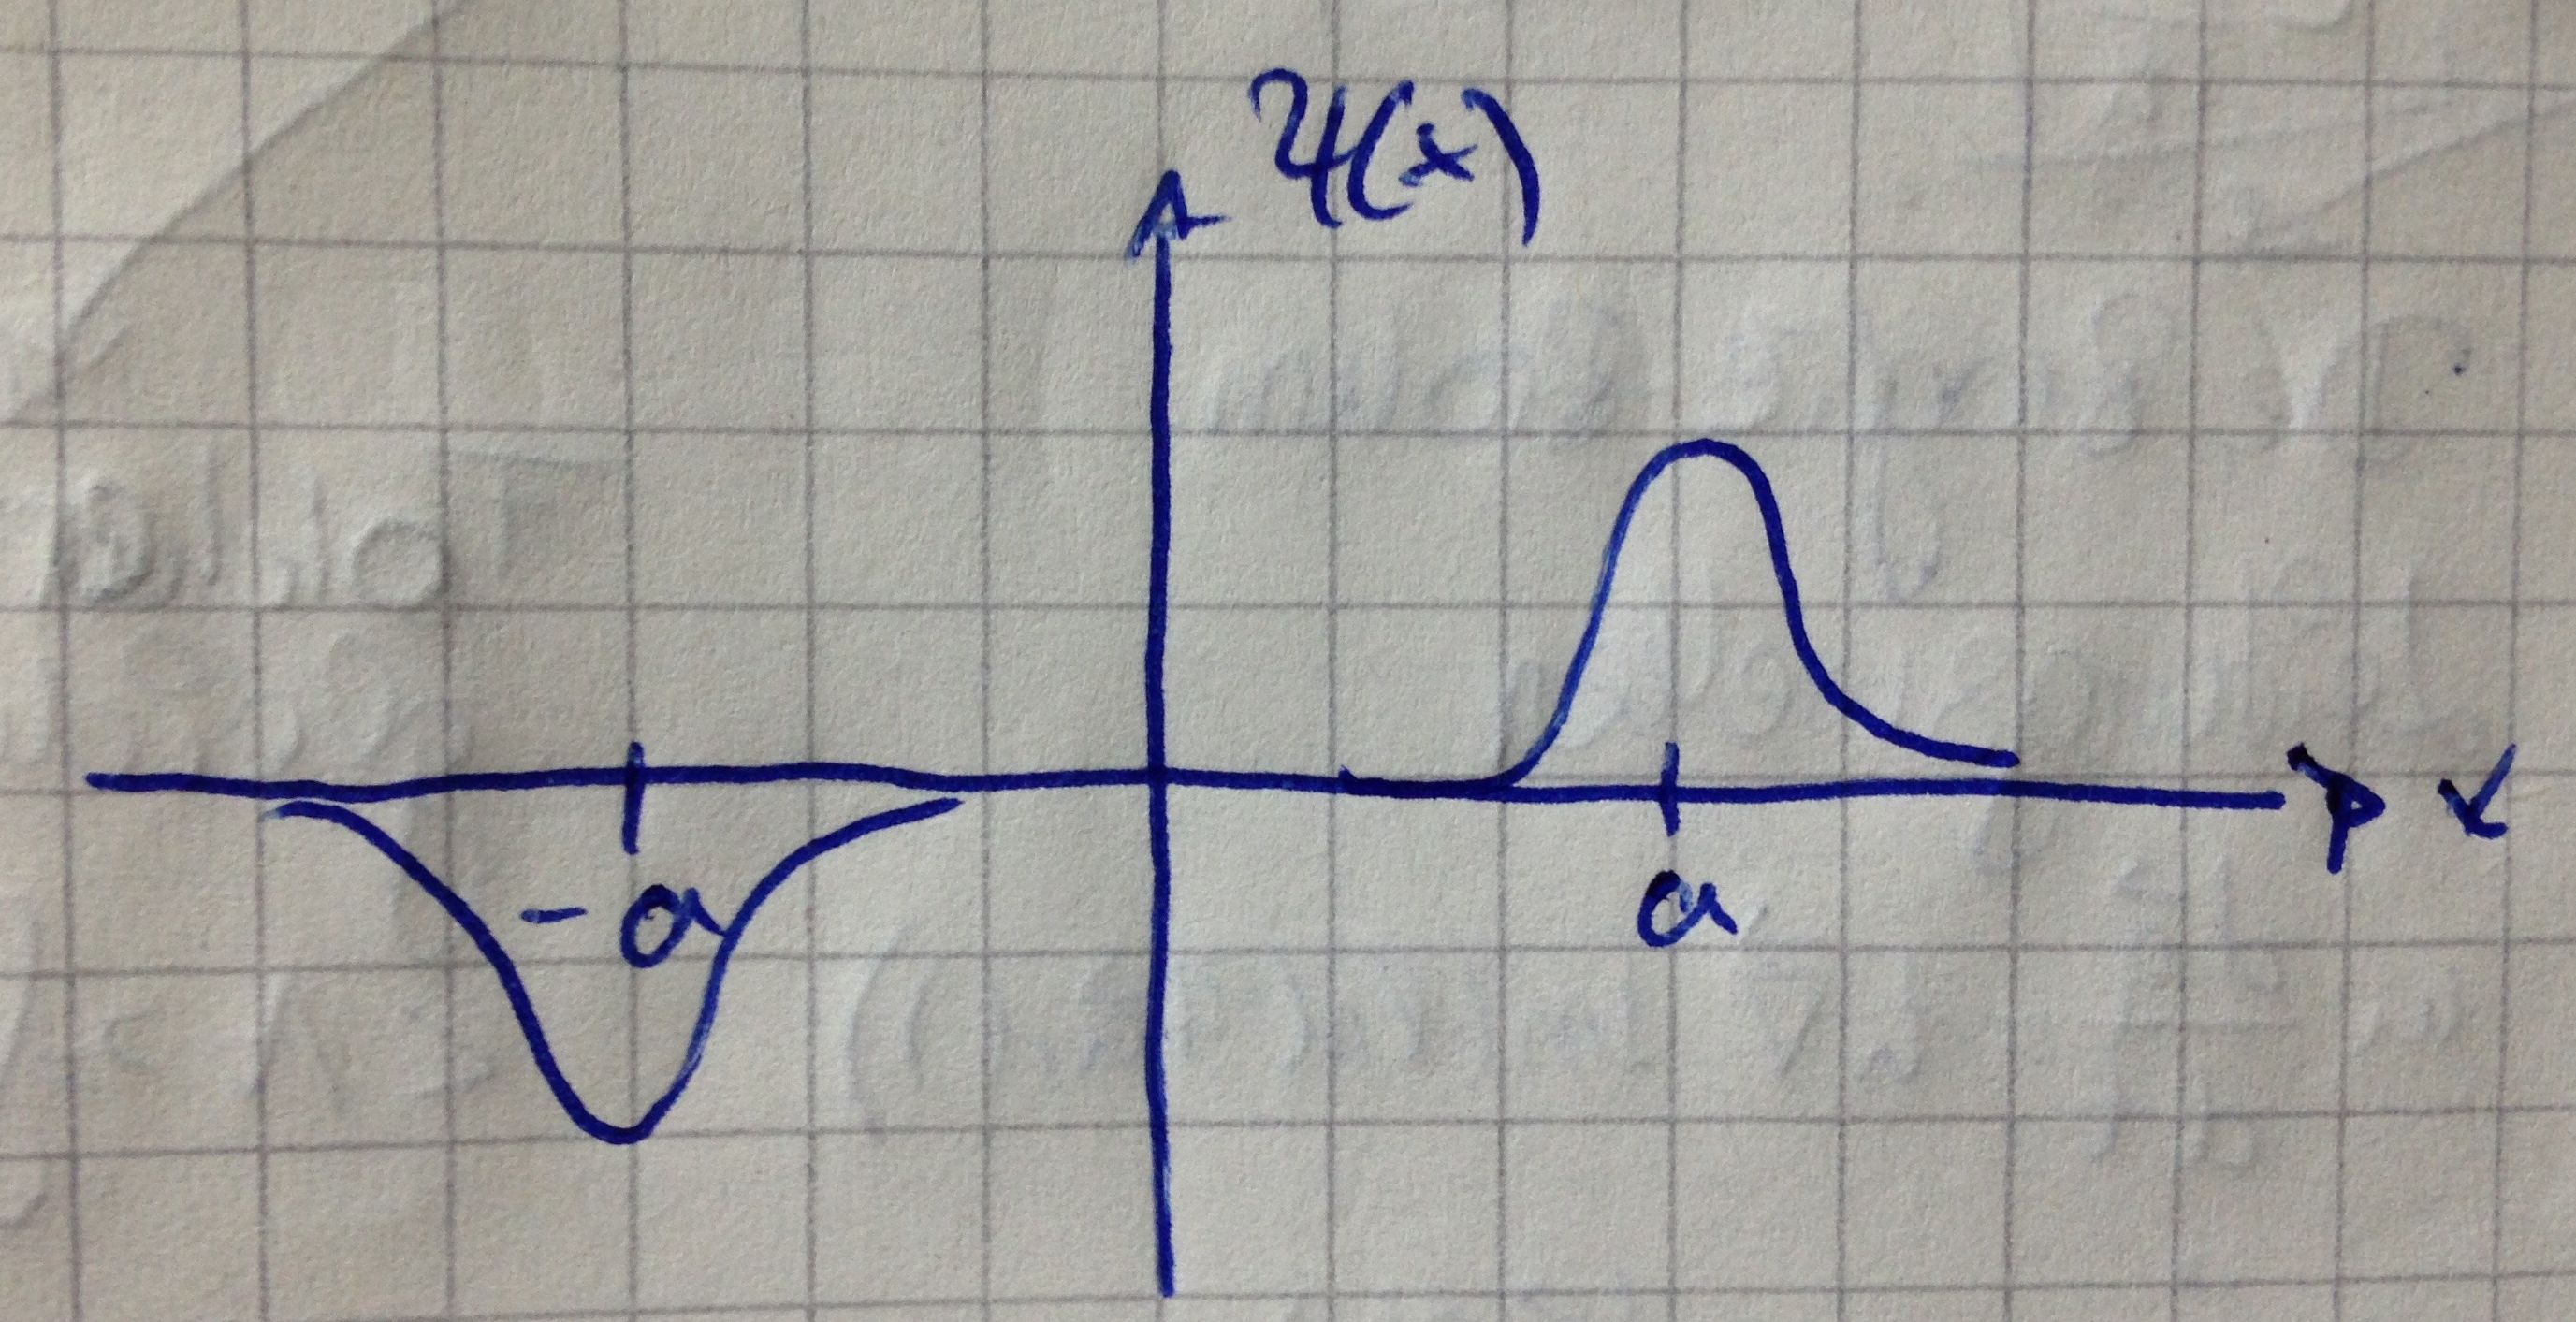
\includegraphics[width= 0.6\textwidth]{Tunneln_durch_eine_Potentialbarriere3}
		\end{center}
	\end{figure}
\FloatBarrier
Definiere $\ket{+}$	und $\ket{-}$
	\begin{figure} [h]
		\begin{center}
			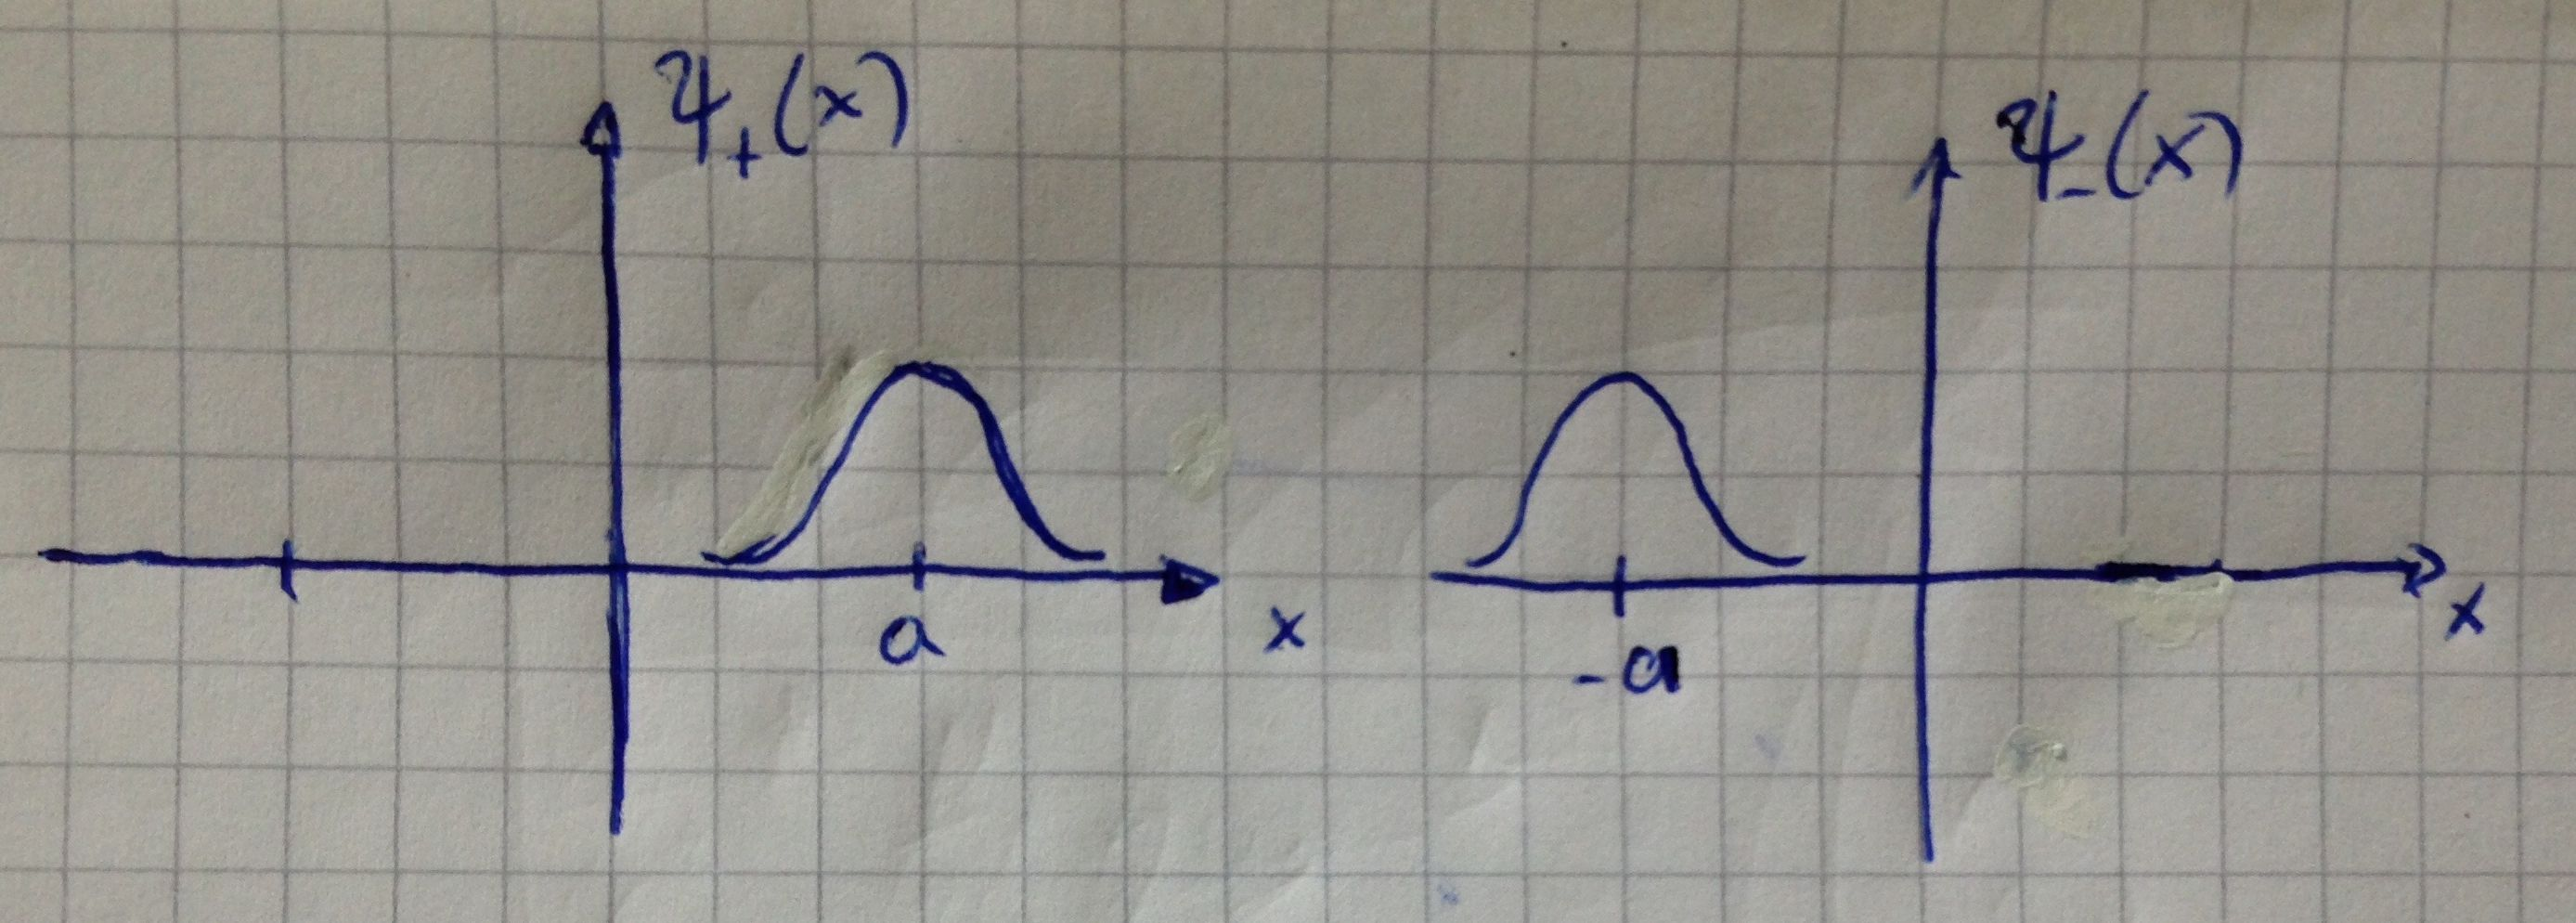
\includegraphics[width= \textwidth]{Tunneln_durch_eine_Potentialbarriere4}
		\end{center}
	\end{figure}
\FloatBarrier
	\begin{align*}
		\ket{0} &\approx \frac{1}{\sqrt{2}} \left(\ket{+} + \ket{-}\right) \\
		\ket{1} &\approx \frac{1}{\sqrt{2}} (\ket{+} - \ket{-}) \\
		\Delta E &= E_1 - E_0 > 0 
	\end{align*}
Beispiel: Amoniak maser

Tunnelprozesse:
	\begin{align*}
		S_E &= \int \limits_{-\frac{T}{2}}^{\frac{T}{2}} \diff \tau 
		\left(\frac{m}{2} \dot{x}^2 + V(x)\right) & \text{ mit Randbedingung:}&\\
		&&x \left(-\frac{T}{2}\right) &= -a ,~ x \left(\frac{T}{2}\right) = a \\
		\braket{+ | -} &= \int [\diff x] e^{-S_E[x]}
	\end{align*}
	\begin{figure} [h]
		\begin{center}
			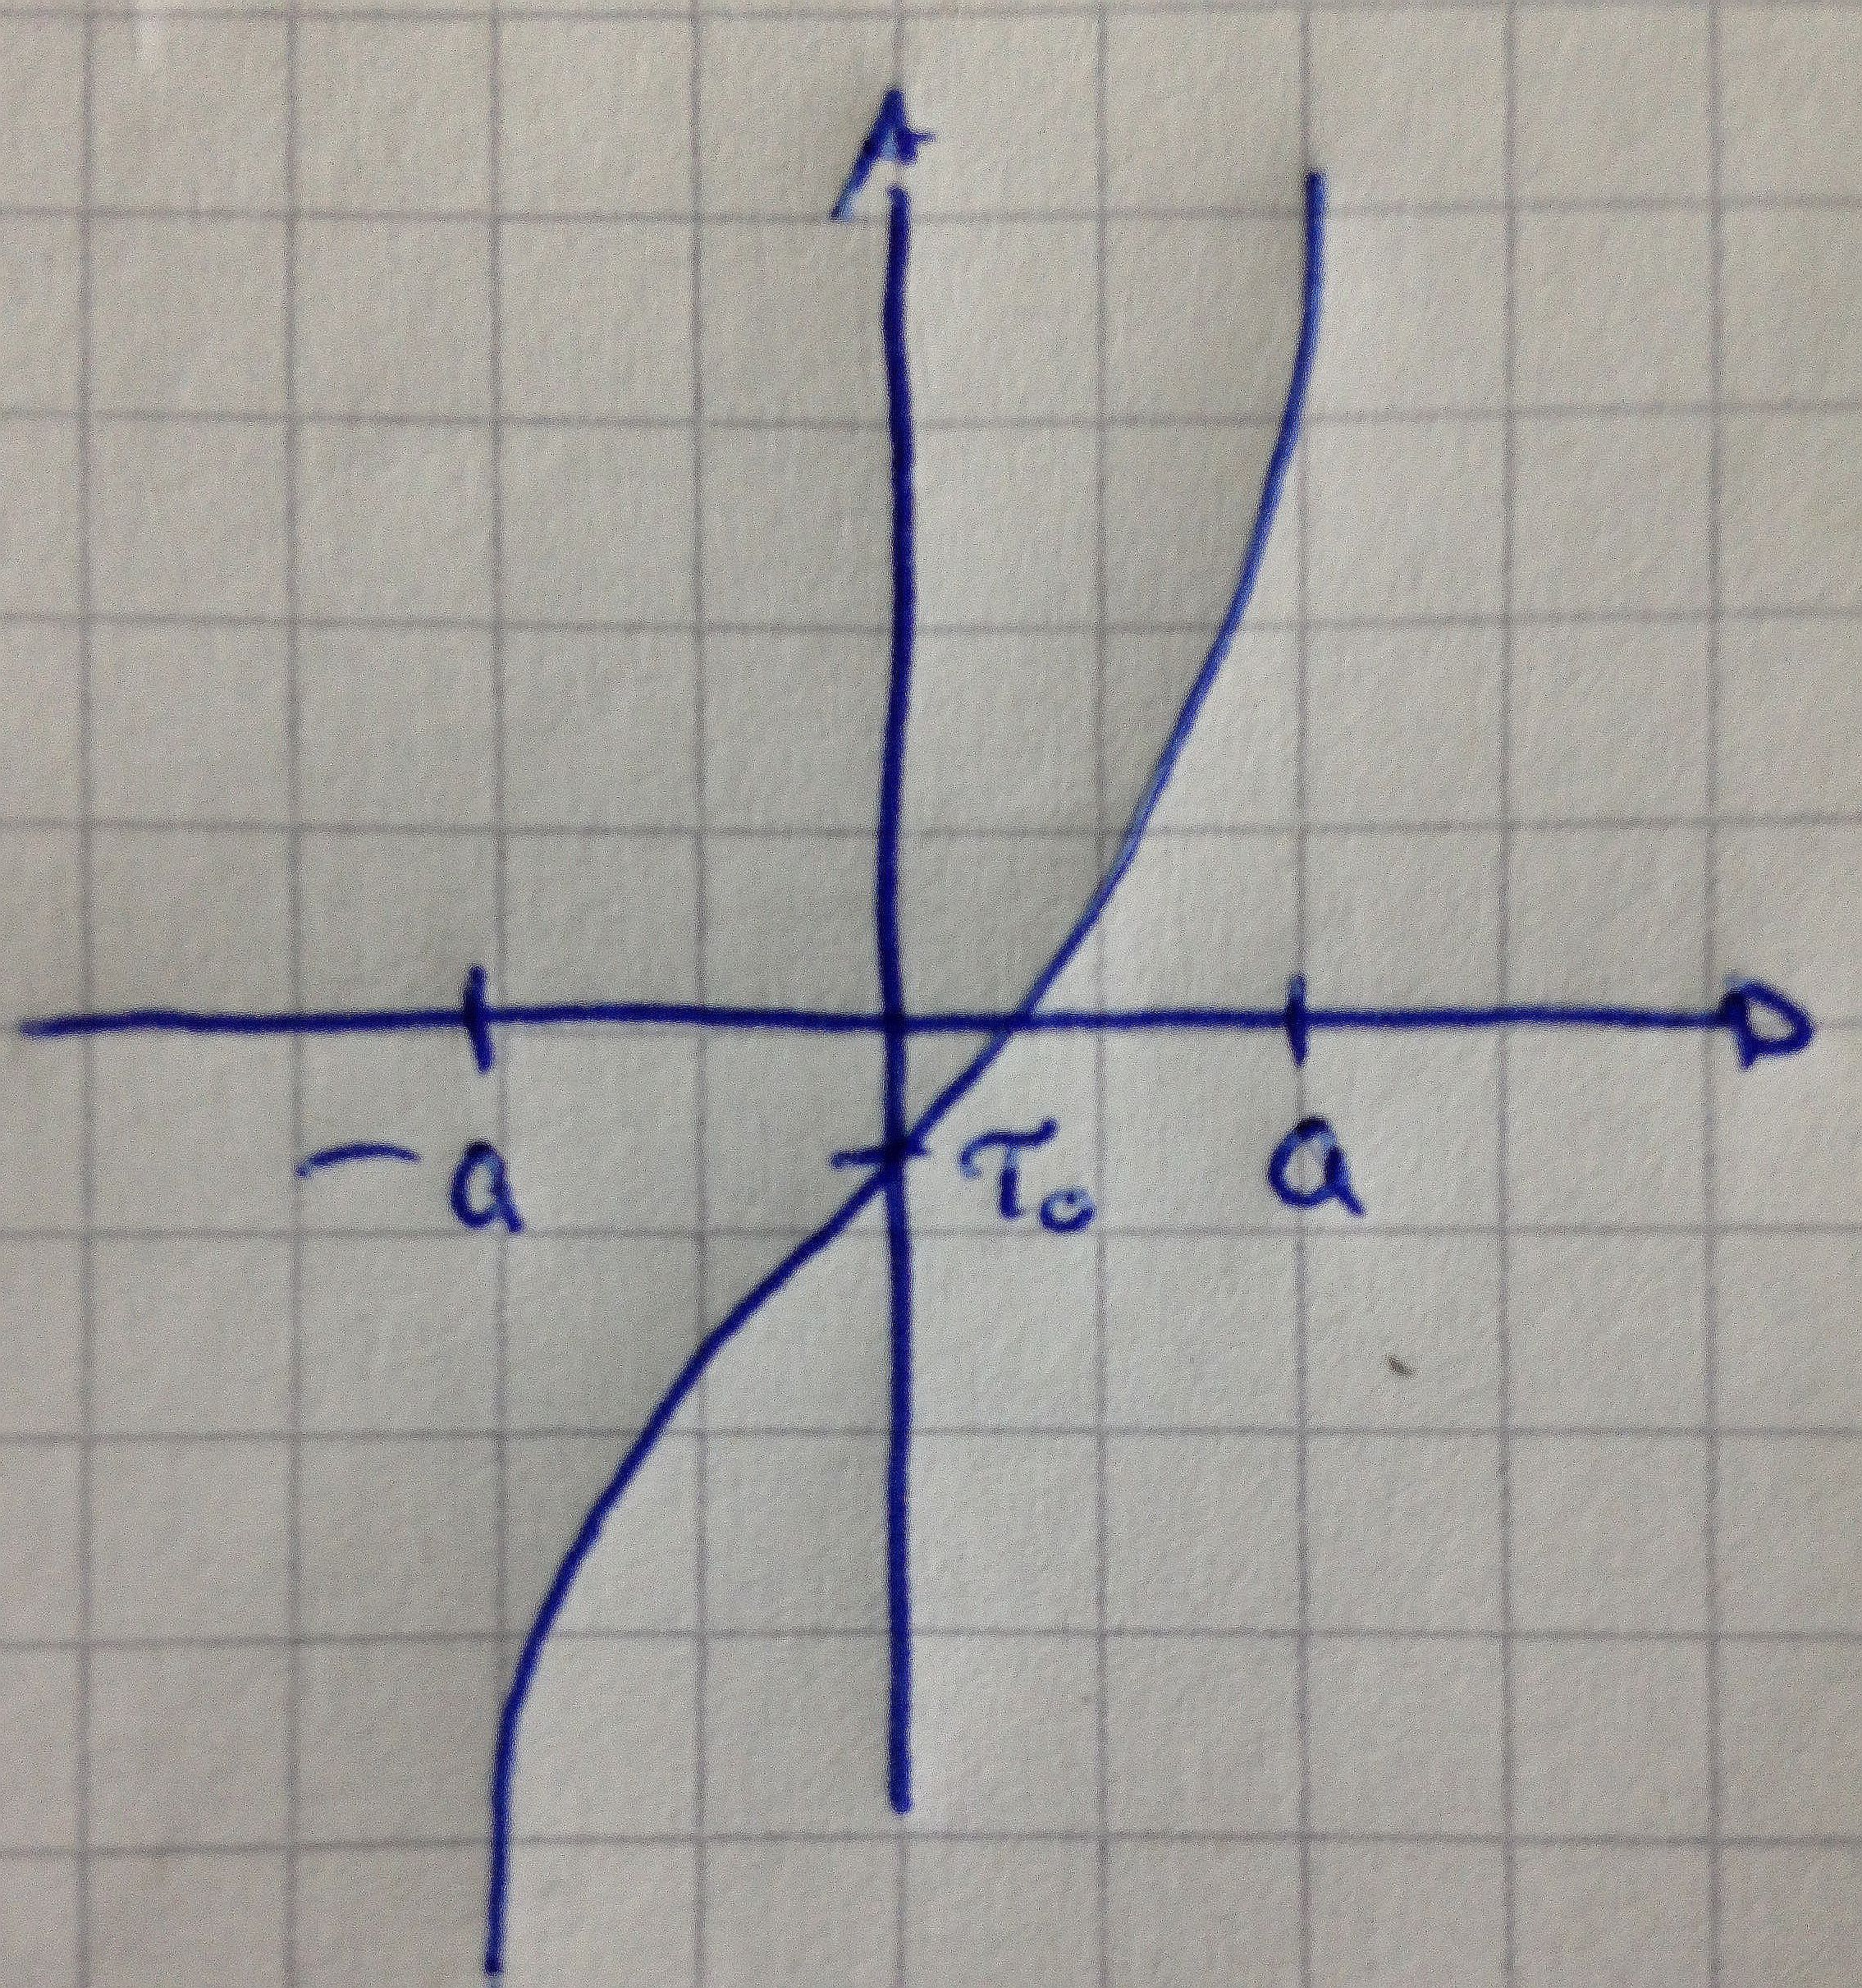
\includegraphics[width= 0.4\textwidth]{Tunneln_durch_eine_Potentialbarriere5}
		\end{center}
	\end{figure}
	\begin{align*}
		\Delta E &= -2 \braket{+ | H | -} \sim \int [\diff x] e^{-S_E[x]}
	\end{align*}
Semiklassische Näherung: Nehme klassische Pfade und addiere Fluktuationen um klassische Pfade: 
	\begin{align*}
		x(\tau) &= x_c(\tau) + y(\tau) \\
		\frac{\delta S_E}{\delta x_c(\tau)} &= 0
		&\Rightarrow m \ddot{x}_c = V' (x_c) 
	\end{align*}
kein Minus wegen der euklidischen Zeit. Wie Newton-Bewegungsgleichung, aber mit $V \mapsto -V$
	\begin{figure} [h]
		\begin{center}
			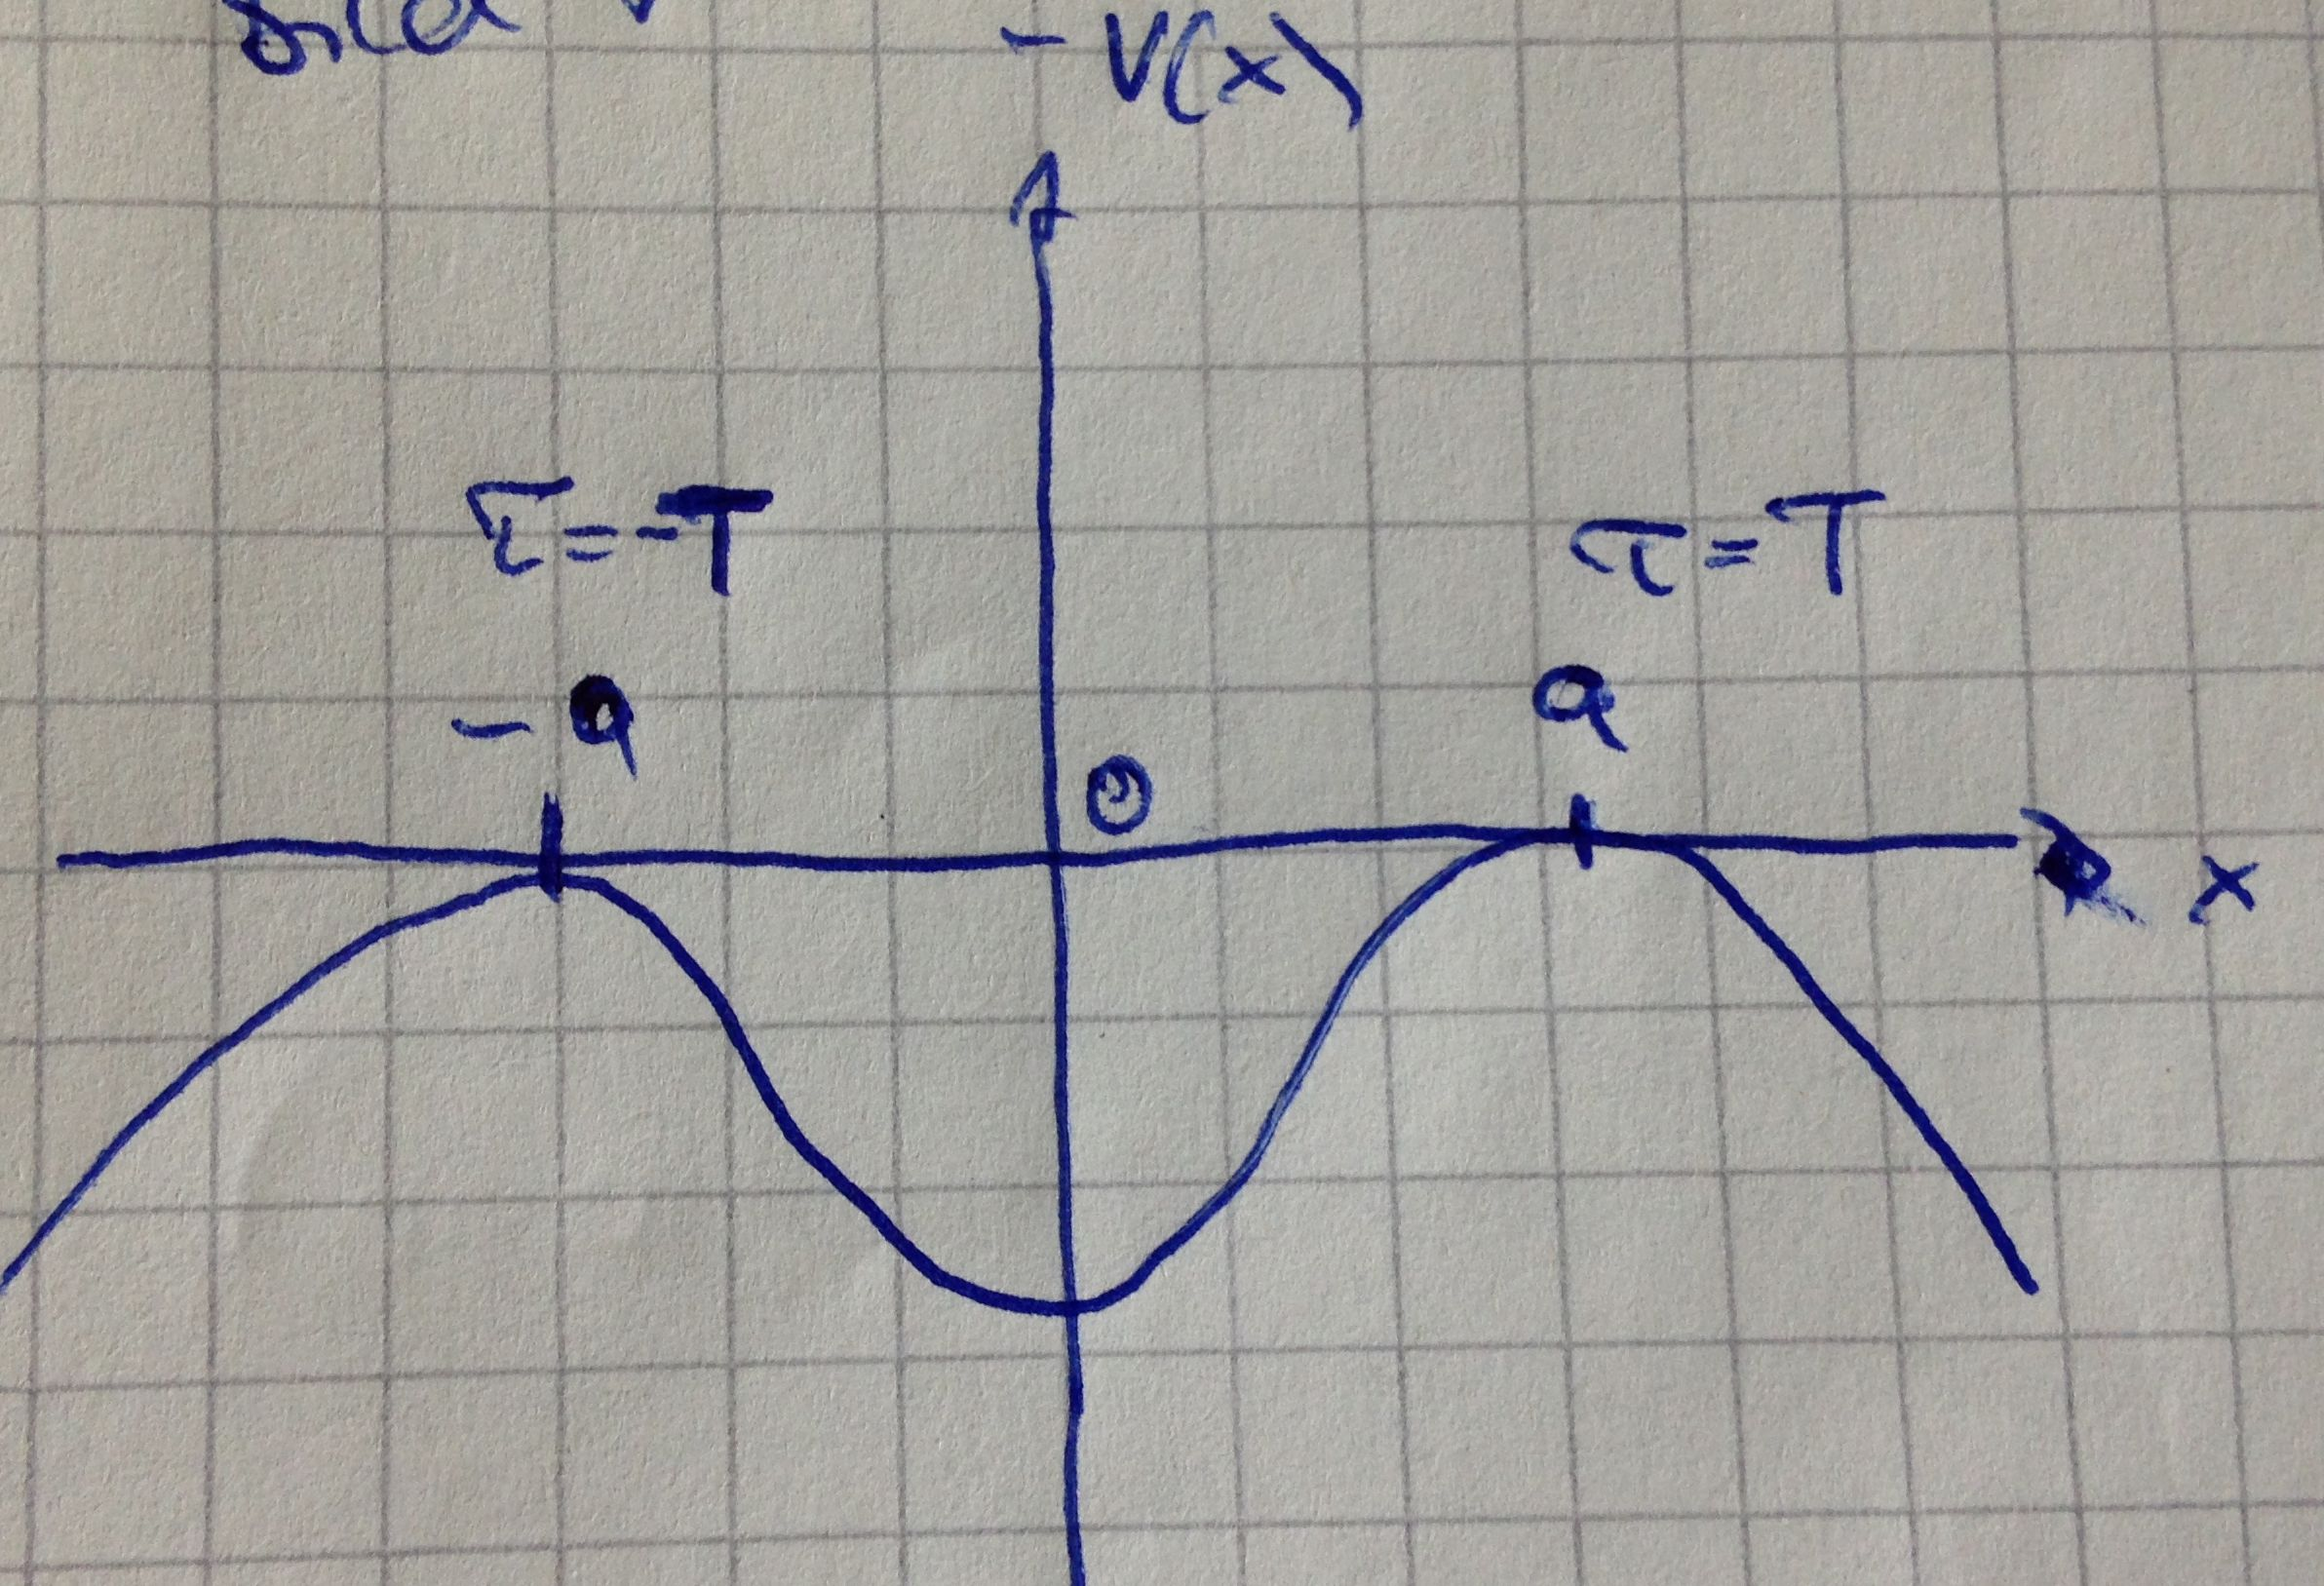
\includegraphics[width= 0.5\textwidth]{Tunneln_durch_eine_Potentialbarriere6}
		\end{center}
	\end{figure}
	\begin{align*}
		\mathrm{T} \rightarrow \infty &: 
		x_c(\tau) = a \tanh \left[\frac{\omega}{2} (\tau- \tau_0)\right] \\
		m \omega^2 &= V^{''}(a) = 8 \lambda a^2
		\Rightarrow a^2 = \frac{m \omega^2}{8 \lambda}
	\end{align*}
je größer $\lambda$ desto ``eckiger'' wird der Pfad bei $\tau_0$ 
\\

$\omega$ klein ($\lambda a^2$ klein)
	\begin{figure} [h]
		\begin{center}
			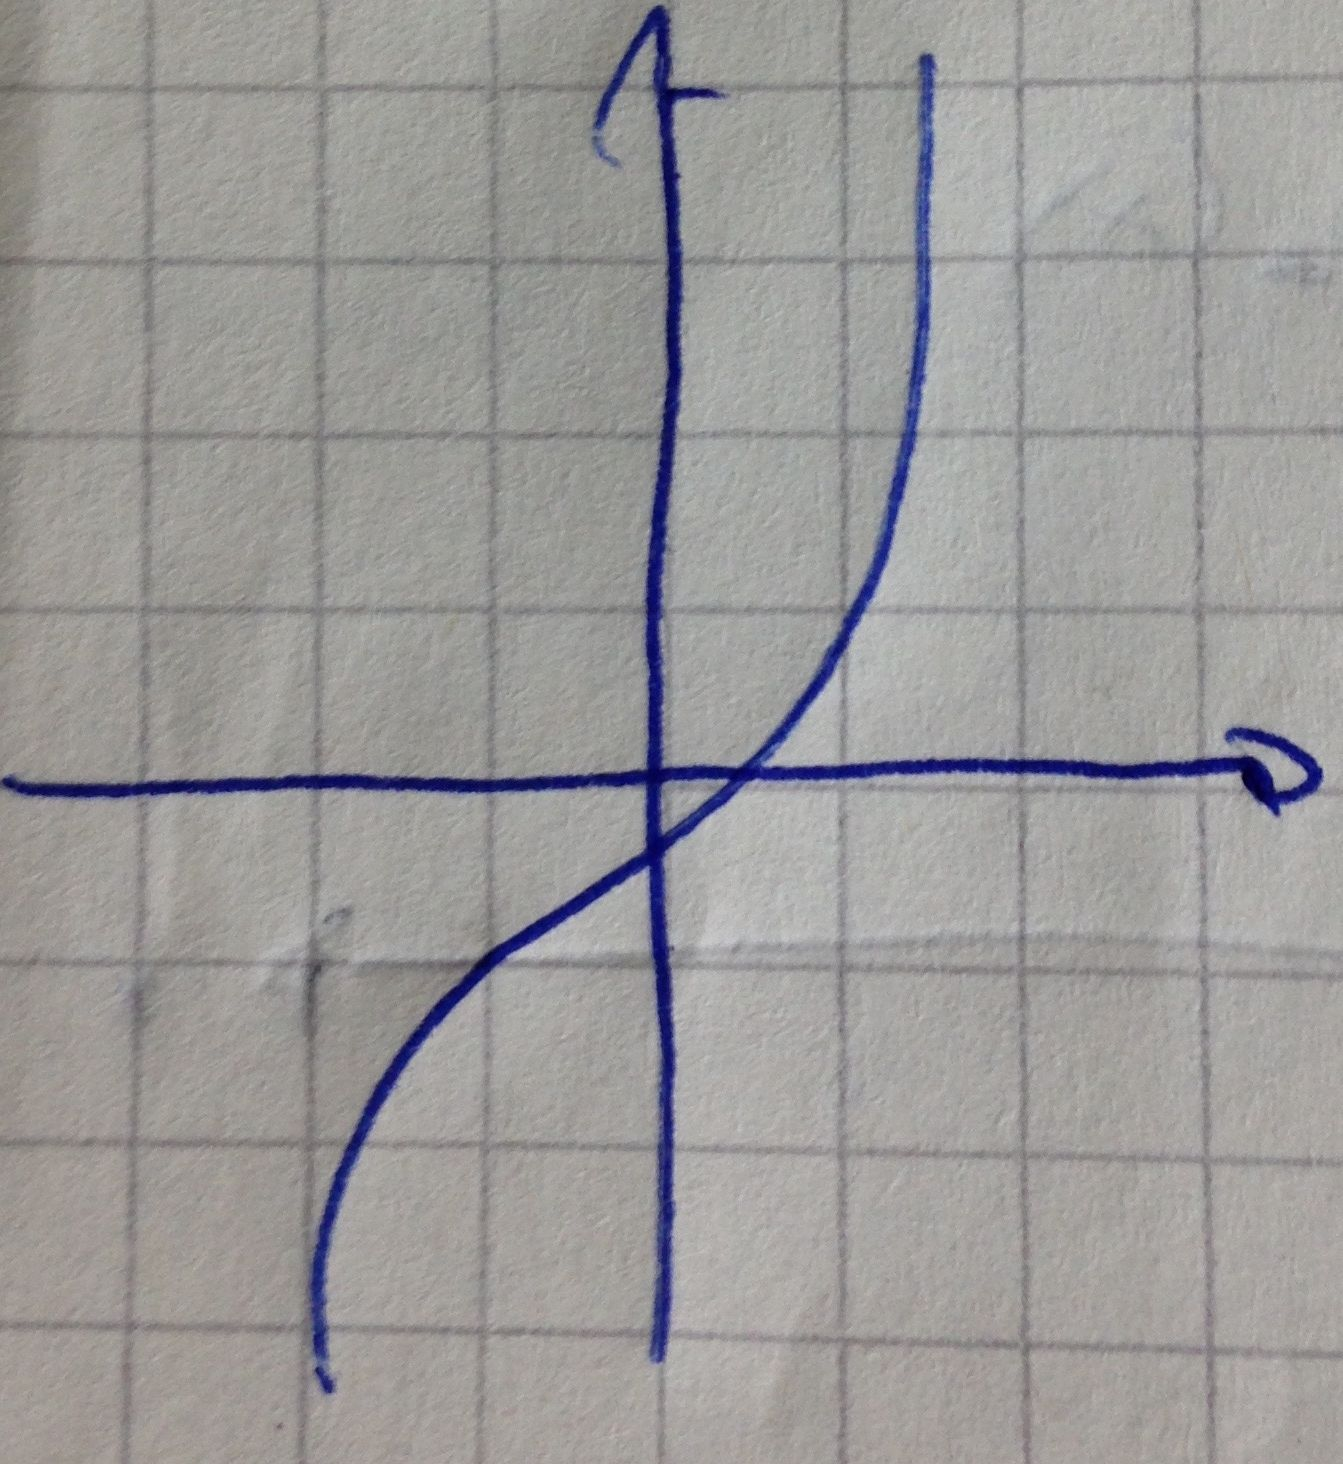
\includegraphics[width= 0.4\textwidth]{Tunneln_durch_eine_Potentialbarriere7}
		\end{center}
	\end{figure}
\FloatBarrier		
$\omega$ groß
	\begin{figure} [h]
		\begin{center}
			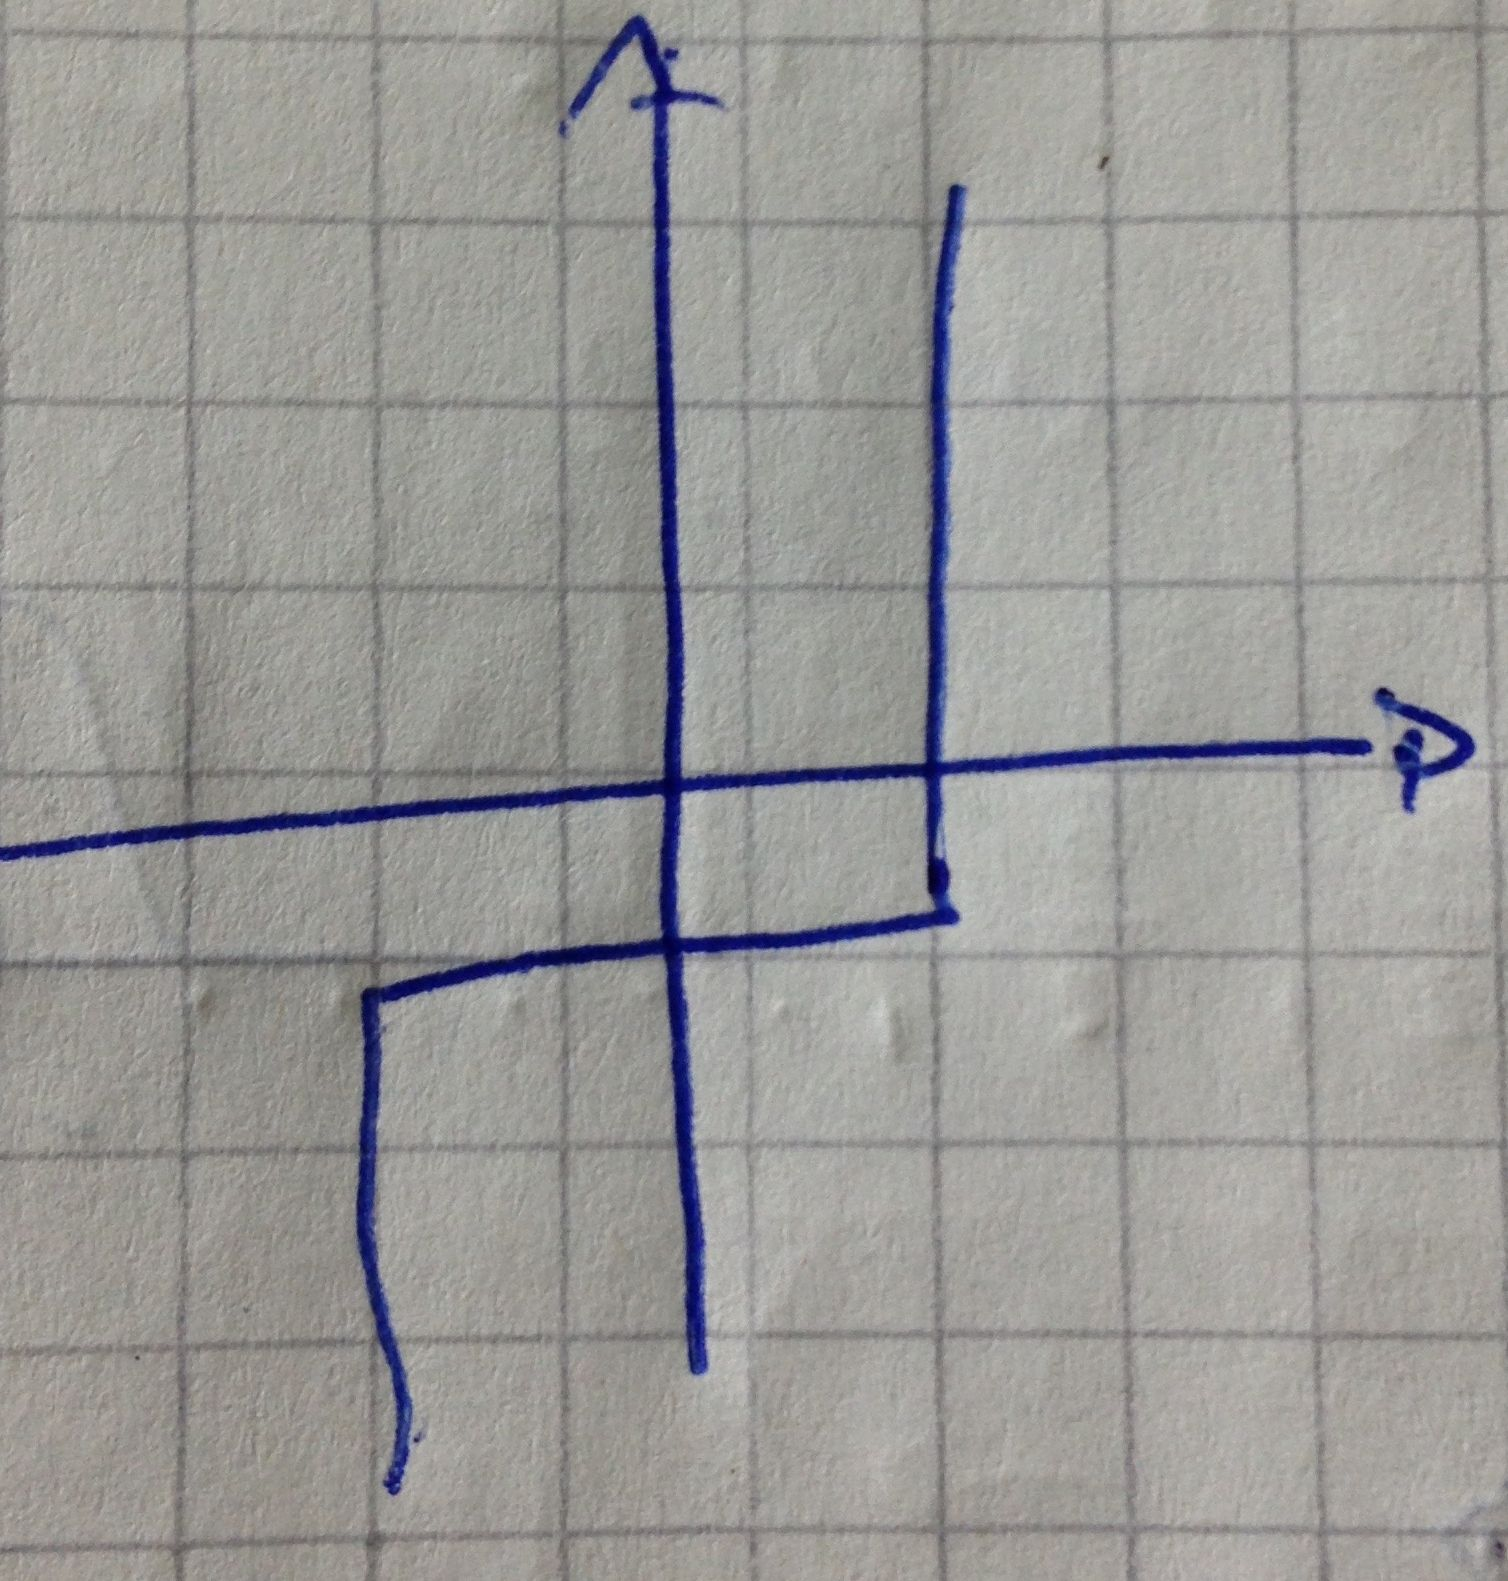
\includegraphics[width= 0.4\textwidth]{Tunneln_durch_eine_Potentialbarriere8}
		\end{center}
	\end{figure} 
\FloatBarrier
Kink (Knick) Lösung
	\begin{align*}
		\frac{m}{2} \dot{x}^2 - V(x) &= 0 
	\end{align*}
(euklidische Energieerhaltung)
	\begin{align*}
		S_E[x_c] &= \int\limits_{-\infty}^{\infty} \diff \tau
		\left[\frac{m}{2} \dot{x}^2 + V(x(\tau))\right] = \\
		&=\int \limits_{-\infty}^\infty \diff \tau m\dot{x}^2
		= \int \limits_{-a}^a \diff x m \dot{x}
		= \int \limits_{-a}^a \diff x \sqrt{2m V(x)} \\
		S_E[x_c] &= \frac{m^2 \omega^2}{12 \lambda} = \frac{4}{3} \sqrt{2m\lambda} a^3
	\end{align*}
	\begin{align*}
		x(\tau) &= x_c (\tau) + y(\tau) \\
		S_E[x] &= S_E [x_c] + \frac{1}{2} \int \diff \tau_1 \diff \tau_2 
		y(\tau_1) A(\tau_1, \tau_2) y(\tau_2) + \ldots \\
		\Delta E &\sim \int [\diff x] e^{-S_E[x]} 
		\Rightarrow \Delta E \approx N e^{-S_E[x_c]} (\det(A))^{-\frac{1}{2}} \\
		\Delta E &\approx K \underbrace{e^{- \int_{-a}^{a} \diff x \sqrt{2m V(x)}}}_{\mathclap{\text{Gamov-Faktor}}}
		= K e^{-\frac{m^2\omega^3}{12 \lambda}} \\
		K &= \frac{N}{\sqrt{\det A}} = 2 \sqrt{\frac{m^2 \omega^5}{2 \pi \lambda}}
	\end{align*}
	\subsection{Zugänge zur Quantenmechanik}
\FloatBarrier
	\begin{figure} [h]
		\begin{center}
			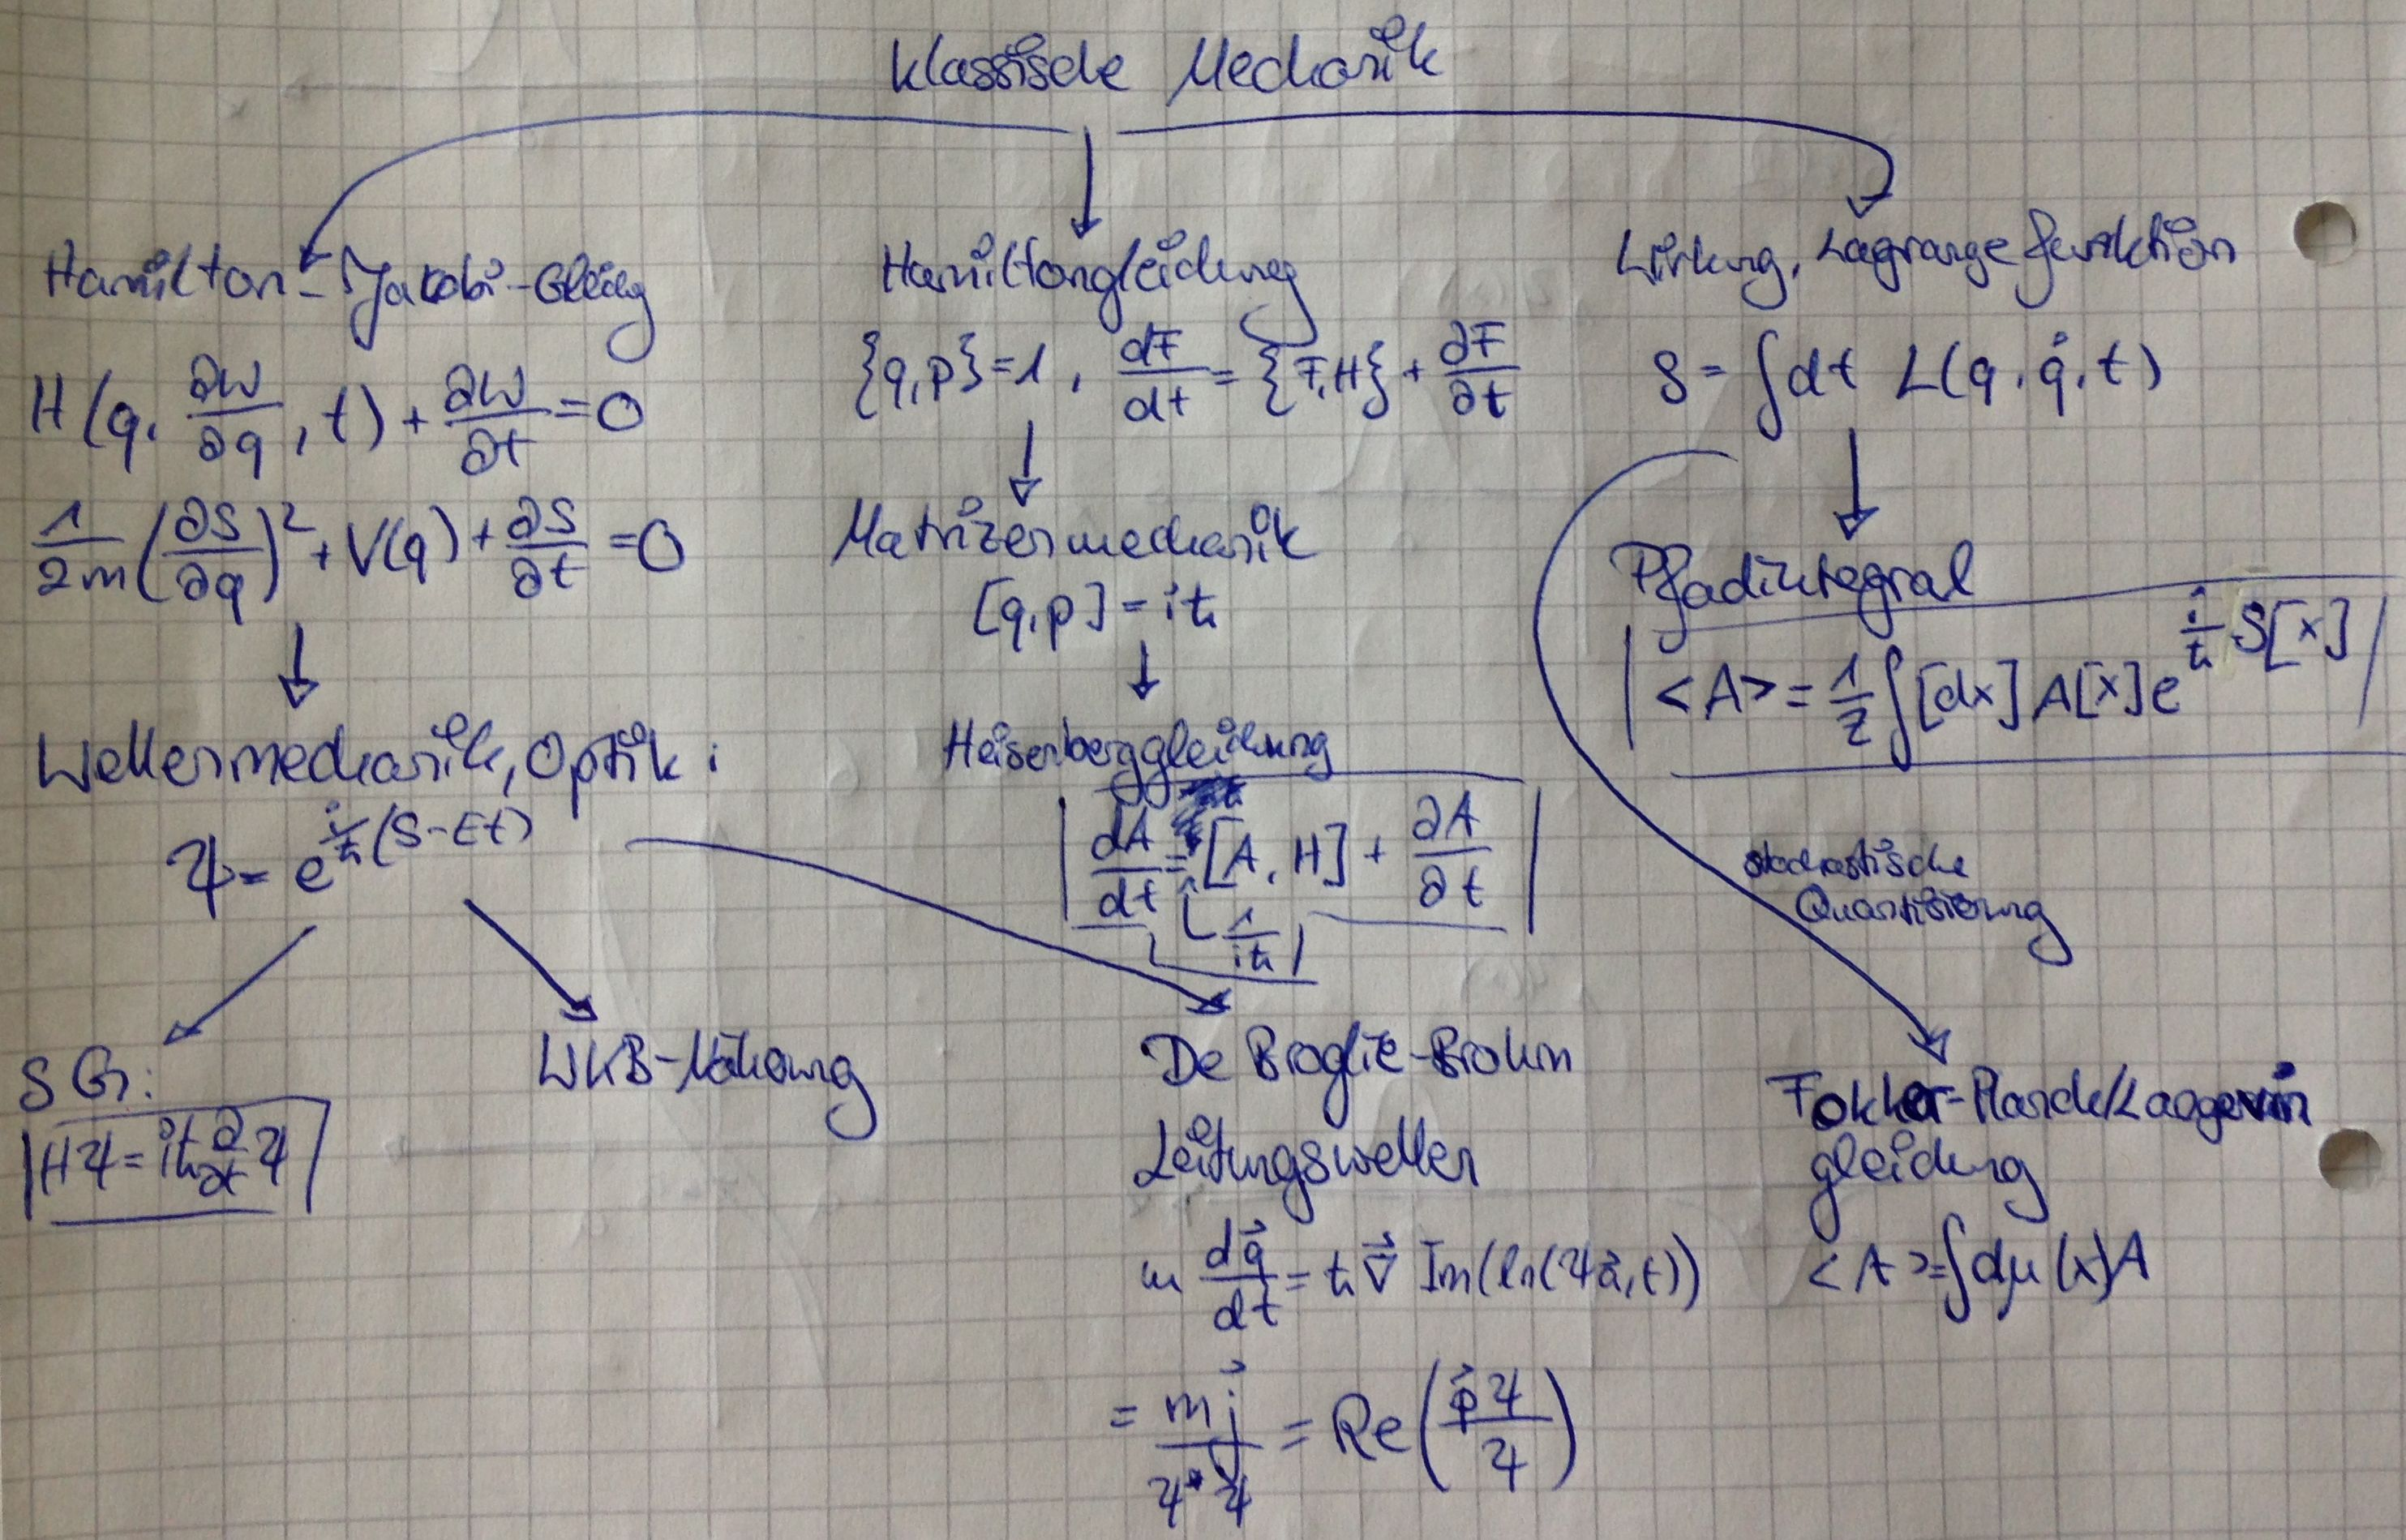
\includegraphics[width = 0.9\textwidth]{Zugaenge_zur_Quantenmechanik1}
		\end{center}
	\end{figure} 
	%Kap6
	\section{Konzeptionelle Fragen der Quantenmechanik} \marginpar{07.01.2016}
	\begin{itemize}
		\item Bedeutung von ``Wahrscheinlichkeiten''
		\item Der Messprozess
		\item ``Verschränkte'' Zustände + Korrelation
	\end{itemize}
	\subsection{Reine Zustände} 
Wiederholung: Quantenmechanik Regeln
	\begin{enumerate}[1.]
		\item Vorhersagen von Messergebnissen an einem ansonsten isolierten System sind probabilistisch. In Situationen, in denen die \underline{maximal mögliche} Information bekannt ist, kann diese dargestellt werden durch einen Vektor/Strahl $\ket{\psi}$ in einem komplexen Hilbertraum $\Hil$.
		\item Jede Observable $A$ kann dargestellt werden als selbstadjungierter Operator $\hat{A}$, welcher auf Vektoren in $\Hil$ wirkt.
		
		(NB: $\vec{x}$ ist z.B. keine echte Observable, da nicht-normierbarer Eigenvektor (uneigentlich). Es existiert auch kein Messinstrument, mit welchem sich $\vec{x}$ beliebig genau bestimmen lässt.)
		\item Erwartungswert einer Messung von $A$: $\erw{A}_\psi = \braket{\psi | A | \psi}$
		\item In einem \underline{abgeschlossenen} System ist
			\begin{align*}
				i \hbar \frac{\diff}{\diff t} \ket{\psi (t)} = \hat{H} \ket{\psi(t)}
			\end{align*}
		$\hat{H}$ : Hamiltonoperator
		\begin{enumerate}[(a)]
			\item Einzigen möglichen Messergebnisse von $A$ sind Eigenwerte (EW) $a_i$ von $\hat{A}$.
			\item Wahrscheinlichkeit
				\begin{align*}
					&W(A = a_n \ket{\psi}) = \braket{\psi | \hat{P}_n | \psi} \\
					\text{mit}~
					&\boxed{\hat{P}_n = \sum_{j = 1}^{dim (n)} \ket{a_n, j} \bra{a_n, j}}
					~\text{: Projektor}
				\end{align*}
			$dim$ von Eigenwert zum EW $a_n$ (Entartung)
			
			(NB: $\braket{\psi | \hat{P}_n | \psi} = \sum_{j= 1}^{dim(n)}|\braket{a_n, j | \psi}|^2$)
			
			Beweis: Statistsisches Mittel
				\begin{align*}
					\erw{F(A)} = \sum_m F(\alpha_m) W(A = \alpha_m)
				\end{align*}
				
			Beispiel für $\mathscr{F}$:
				\begin{align*}
					\chi_r (A) &= 
					\left\{
					\begin{aligned}
						1&, A = r \\
						0&, A \neq r
					\end{aligned}
					\right. \\
					\Rightarrow W (A = r) &= \erw{\chi_r (A)} \\
					\text{QM: } \\
					\erw{\mathscr{F}(A)}_\psi &= \sum_m \mathscr{F}(\alpha_m) W(A = \alpha_m; \ket{\psi}) \\
					\erw{\chi_r(A)} &\underset{\text{Regel 3}}{=}
					\braket{\psi | \chi_r(\hat{A}) | \psi} = \sum_m \chi_r (\alpha_m) W(A = \alpha_m ; \ket{\psi}) \\
					\chi_r (\hat{A}) &= \sum_m \chi_r (a_m) \hat{P}_m \\
					\Rightarrow \sum_m \chi_r (a_m) \braket{\psi | \hat{P}_m | \psi} 
					&= \sum_m \chi_r (\alpha_m) W(A = \alpha_m; \psi) \\
					\braket{\psi | \hat{P}_m | \psi} &=
					\left\{
					\begin{aligned}
						\braket{\psi | \hat{P}_m | \psi} &, a_m = r \\
						0 &, \text{ sonst}
					\end{aligned}
					\right. \\
					W(A = \alpha_m; \psi) &=
					\left\{
					\begin{aligned}
						W(A = \alpha_m; \psi) &, \alpha_m = r \\
						0 &, \text{ sonst}
					\end{aligned}
					\right.
				\end{align*}
				$\Rightarrow$
				\begin{enumerate}[(a)] 
					\item $\alpha_m = a_m$
					\item $\braket{\psi | \hat{P}_m | \psi} = 
					W(A = a_m ; \ket{\psi}) = 
					\sum_{j = 1}^{dim(m)} |\braket{a_m, j | \psi}|^2$
				\end{enumerate}
				\begin{align*}
				\mathds{1} \underset{\text{weil } \ket{a_m, j} \text{ Basis von }\Hil}{=}
				\sum_m \hat{P}_m \Rightarrow
				1 = \braket{\psi | \psi} &= \sum_m \braket{\psi | \hat{P}_m | \psi} 
				= \sum_m W(A = a_m ; \ket{\psi}) \\
				\sum \text{ Wahrscheinlichkeiten} &= 1 \checkmark \\
				\hat{P}_m \text{ist ``Projektionsoperator''}& \\
				\hat{P}_m^2 = \sum_{j, k = 1}^{dim(m)} \ket{a_m, j} \braket{a_m j | a_m, k} \bra{a_m, k} &= \hat{P}_m
				\end{align*}
				$\hat{P}^2 = \hat{P} \Rightarrow$ Nur Eigenwerte 0 oder 1 sind möglich
		\end{enumerate}
	\end{enumerate}	
\subsection{Statistische Gemische und Dichtematrix}
	Beispiel: Wir wissen, dass ein System mit einer Wahrscheinlichkeit $W_1$ sich in einem quantenmechanischen Zustand $\ket{\psi_1}$ und $W_2$ in $\ket{\psi_2}$ etc. befindet.
	
	Man nennt dies ein statistisches Gemisch:
		\begin{align*}
			(\ket{\psi_1}, \ket{\psi_2}, \ldots; W_1, W_2, \ldots) \text{ mit } \sum_d W_{d} = 1.
		\end{align*}
	Die $W_d$ sind \underline{klassische} Wahrscheinlichkeiten, die additiv sind. Sie haben ihren Ursprung z.B. in nicht-perfekten Instrumenten bei der Präsentation eines Zustands
	$\Rightarrow$ von Regel 3.
	\subsubsection*{Stern-Gerlach Experiment}
%		\begin{figure}
%			\begin{center}
%				\includegraphics[content...]{imagefile}
%			\end{center}
%		\end{figure}
	Was ist mit Gemischen?
	\begin{align*}
		\alpha \ket{\uparrow} &+ \beta \ket{\downarrow},& \alpha^2 + \beta^2 &= 1 \\
		W_\uparrow\ket{\uparrow} &+ W_\downarrow \ket{\downarrow},& W_\uparrow + W_\downarrow &= 1.
	\end{align*}
	\begin{align*}
		W(A = a_n; \ket{\psi}) &= \braket{\psi | \hat{P}_n | \psi} \\
		\rho &\coloneqq (\ket{\psi_1}, \ket{\psi_2}, \ldots; W_1, W_2, \ldots) \\
		W(A=a_m; \rho) &= \sum_{d} W_d (A = a_m ; \ket{\psi_d}) \\
		&= \sum_d W_d \braket{\psi_d | \hat{P_n} | \psi_d} 
	\end{align*}
	Grundannahme: quantenmechanische und klassische Wahrscheinlichkeiten sind unkorreliert
	
	Basis $\{\ket{e_1}, \ket{e_2}, \ldots \}$ von $\Hil$
		\begin{align*}
			\mathrm{Sp } \hat{B} &\coloneqq \sum_i \braket{e_i | \hat{B} | e_i} &
			\sum_i \ket{e_i} \bra{e_i} &= \mathds{1} \\
			\braket{\psi| \hat{B} | \psi} &= 
			\sum_i \braket{\psi | \hat{B} | e_i} \braket{e_i | \psi} \\
			&= \sum_i \braket{e_i | \psi} \braket{\psi | \hat{B} | e_i} \\
			&= \mathrm{Sp }(\ket{\psi} \bra{\psi} \hat{B}) \\
			&= \mathrm{Sp } (\hat{P}_{\ket{\psi}} \hat{B}) &
			\text{mit } \hat{P}_{\ket{\psi}} &= \ket{\psi} \bra{\psi} 
		\end{align*}
	$\hat{P}^2_{\ket{\psi}} =\hat{P}_{\ket{\psi}}$ weil $\braket{\psi | \psi} = 1$
	
	Analog:
		\begin{align*}
			W(A = a_n; \ket{\psi}) &= \braket{\psi | \hat{P}_n | \psi} = 
			\mathrm{Sp } \hat{P}_{\ket{\psi}} \hat{P}_n \\
			\erw{A}_\psi &= \mathrm{Sp} \, (\hat{P}_{\ket{\psi}}, \hat{A}) 
		\end{align*}
	Dichte - ``Matrix'':
		\begin{align*}
			\boxed{
					\hat{\rho} \coloneqq \sum_d W_d \hat{P}_{\ket{\psi_d}} = 
					\sum_d W_d \ket{\psi_d} \bra{\psi_d}
				}
		\end{align*}
		\begin{align*}
			W(A = a_n; \rho) &= \sum_d W_d \mathrm{Sp}\, (\hat{P}_{\ket{\psi_d}} \hat{P}_n) \\
			&= \mathrm{Sp}\, \left(
				\left(
					\sum_d W_d \hat{P}_{\ket{\psi_d}} 
				\right) \hat{P}_n
			\right)
		\end{align*}
	Wahrscheinlichkeit bei Messung von $A$ auf Gemisch $\rho$ das Ergebnis $a_n$ zu finden:
		\begin{empheq}[box = \boxed]{align*}
			W(A = a_n; \rho) &= \mathrm{Sp} \, (\hat{\rho} \hat{P}_n)\\
			\erw{A}_\rho = \mathrm{Sp}\, (\hat{\rho} \cdot \hat{A}) 
		\end{empheq}	
		\begin{align*}
			\mathrm{Sp}\, \hat{\rho} &= \sum_d W_d = 1 \\
			\mathrm{Sp}\, (\hat{\rho}^2) &\leq 1
		\end{align*}
	Eigenschaften der Dichtematrix eines Gemisches $\rho$:
		\begin{enumerate}[1.]
			\item $\hat{\rho} = \hat{\rho}^\dagger$
			\item $\braket{\psi | \hat{\rho} | \psi} \geq 0 ~\text{für alle} \ket{\psi} \in \Hil$ 
			\item $\mathrm{Sp}\, \hat{\rho} =1$.
			\item $\mathrm{Sp}\, \hat{\rho}^2 \leq 1, ~
			\mathrm{Sp}\,\hat{\rho}^2 \Leftrightarrow \rho$ ist ein Reiner Zustand
		\end{enumerate}
	Beispiel
		\begin{align*}
			S_z &= \frac{\hbar}{2} \sigma_z =
			\begin{pmatrix}
				1 & 0 \\
				0 & -1
			\end{pmatrix} ,&
			S_x &= \frac{\hbar}{2} 
			\begin{pmatrix}
				0 & 1 \\
				1 & 0 
			\end{pmatrix} \\
			&\text{EV} : 
			\begin{pmatrix}
			1 \\
			0 
			\end{pmatrix},
			\begin{pmatrix}
			0 \\
			1
			\end{pmatrix} 
			& &\frac{1}{\sqrt{2}}
			\begin{pmatrix}
			1 \\
			1 
			\end{pmatrix} ,
			\frac{1}{\sqrt{2}}
			\begin{pmatrix}
			1 \\
			-1
			\end{pmatrix} \\
			\hat{P}_{S_z = \frac{\hbar}{2}} &=
			\begin{pmatrix}
			1 \\
			0
			\end{pmatrix} 
			\begin{pmatrix}
			1 & 0
			\end{pmatrix} =
			\begin{pmatrix}
			1 & 0 \\
			0 & 0
			\end{pmatrix}, &
			\hat{P}_{S_z = -\frac{\hbar}{2}} &= 
			\begin{pmatrix}
				0 & 0 \\
				0 & 1
			\end{pmatrix} \\
			\hat{P}_{S_x = \frac{\hbar}{2}} &= 
			\frac{1}{2} 
			\begin{pmatrix}
				1 \\
				1
			\end{pmatrix} 
			\begin{pmatrix}
			1 & 1
			\end{pmatrix}
			= \frac{1}{2} 
			\begin{pmatrix}
			1 & 1 \\
			1 & 1
			\end{pmatrix}, &
			\hat{P}_{S_x = -\frac{\hbar}{2}} &=
			\frac{1}{2} 
			\begin{pmatrix}
				1 & - 1 \\
				-1 & 1 
			\end{pmatrix}
		\end{align*}
	Dichtematrix
		\begin{align*}
			\hat{\rho} &\coloneqq \frac{1}{2}
			\begin{pmatrix}
			1 & 0 \\
			0 & 1
			\end{pmatrix}
			~ \mathrm{Sp}\, \hat{\rho} = 1 \checkmark \\
			\hat{\rho}^2 &= \frac{1}{4} 
			\begin{pmatrix}
				1 & 0 \\
				0 & 1
			\end{pmatrix}
			\Rightarrow \mathrm{Sp}\, \hat{\rho}^2 = \frac{1}{2} \Rightarrow \text{Gemisch} \\
			\hat{\rho} &= \frac{1}{2} 
			\left(
				\hat{P}_{S_z = \frac{\hbar}{2}} + \hat{P}_{S_z = -\frac{\hbar}{2}}
			\right) =
			\frac{1}{2}
			\left(
				\hat{P}_{S_x = \frac{\hbar}{2}} + \hat{P}_{S_x = -\frac{\hbar}{2}}
			\right) \\
			&= \frac{\alpha}{2}
			\left(
			\hat{P}_{S_z = \frac{\hbar}{2}} + \hat{P}_{S_z = -\frac{\hbar}{2}}
			\right) +
			\frac{1 - \alpha}{2}
			\left(
			\hat{P}_{S_x = \frac{\hbar}{2}} + \hat{P}_{S_x = -\frac{\hbar}{2}}
			\right)
		\end{align*}
	Zerlegung der Dichtematrix nach reinen Zuständen ist nicht eindeutig.
	
	$\{\hat{\rho}_1, \ldots, \hat{\rho}_k\}:$ Dichtematrizen, $\{r_1, \ldots, r_k\}$ positive reelle Zahlen mit $(\sum_{k = 1}^{K} r_k = 1) ~\sum_{k = 1}^{K} r_k \hat{\rho}_k$ ist Dichtematrix, weil 
	
	$\mathrm{Sp}\, (\sum_k r_k \hat{\rho}_k) = 1 \Rightarrow$ Menge aller Dichtematrizen ist konvex.
	
	Lediglich Dichtematrizen reiner Zustände $\hat{P}_{\ket{\psi}} = \ket{\psi} \bra{\psi}$ lassen sich nicht weiter zerlegen.
	
	Vorgriff auf statistische Physik: Thermisches Gemisch
		\begin{align*}
			\hat{\rho}_T &= \frac{e^{-\beta \hat{H}}}{Z (\beta)} ,&
			\beta &= \frac{1}{k T},&
			T&: \text{Temperatur} 
		\end{align*}
	Zustandssumme: 
		\begin{align*}
			Z(\beta) = \mathrm{Sp}\, e^{-\beta \hat{H}} 
			&= \sum_n \braket{E_n | e^{-\beta H} | E_n} \\
			&= \sum_n e^{-\beta E_n} \braket{E_n | E_n} \\
			&= \sum_n e^{-\beta E_n}
		\Rightarrow \mathrm{Sp}\, \hat{\rho}_T = 1 \\
		\hat{\rho}_T &= \sum_n \frac{e^{-\beta E_n}}{Z (\beta)} \ket{E_n} \bra{E_n}
		\end{align*}

	Bsp: $\{\ket{\uparrow}, \ket{\downarrow} \}$ mit Wahrheitswerten $w_1, w_2$ 
		\begin{align*}
			\hat{\rho} &= w_\uparrow \hat{P}_\uparrow + w_\downarrow \hat{P}_\downarrow =
			\begin{pmatrix}
				w_\uparrow & 0 \\
				0 & w_\downarrow 
			\end{pmatrix}&
			\sigma_z &= 
			\begin{pmatrix}
				1 & 0 \\
				0 & -1
			\end{pmatrix} \\
			\erw{S_z} \rho &= 
			\frac{\hbar}{2} \mathrm{Sp}\, (\hat{\rho} \sigma_z) =
			\frac{\hbar}{2} \mathrm{Sp}\, 
			\begin{pmatrix}
			w_\uparrow & 0 \\
			0 & w_\downarrow 
			\end{pmatrix} =
			\frac{\hbar}{2} (w_\uparrow - w_\downarrow) 
		\end{align*}
	Spezialfall: $w_\uparrow = w_\downarrow = \frac{1}{2}$ Isotropes Gemisch $\erw{S_z} = 0$
	\\
	Spezialfall 2: $w_\uparrow = 1, w_\downarrow = 0$ reiner Zustand $\erw{S_z}_{\ket{\uparrow}} = \frac{\hbar}{2}$
	
% nützliche Zeichen:
%\curvearrowright
%\mapsto pfeil mit balken vorne drann
%\leadsto geschwungender pfeil
%\sim
%\gg und \ll für viel größer und kleiner
%\lesssim und \gtrsim für ungefähr kleiner und größer
%\simeq
%\leg und \geq für kleiner gleich und größer gleich
%\int\!\!\!\!\!\!\!\!\!\;\sum komisches Summen und Integralzeichen in einem
%\coloneqq Definitionszeichen
%\perp Senkrechtzeichen
\end{document}




%%% Local Variables: ***
%%% TeX-master: "main.tex" ***
%%% End: ***